% This is the Reed College LaTeX thesis template. Most of the work
% for the document class was done by Sam Noble (SN), as well as this
% template. Later comments etc. by Ben Salzberg (BTS). Additional
% restructuring and APA support by Jess Youngberg (JY).
% Your comments and suggestions are more than welcome; please email
% them to cus@reed.edu
%
% See https://www.reed.edu/cis/help/LaTeX/index.html for help. There are a
% great bunch of help pages there, with notes on
% getting started, bibtex, etc. Go there and read it if you're not
% already familiar with LaTeX.
%
% Any line that starts with a percent symbol is a comment.
% They won't show up in the document, and are useful for notes
% to yourself and explaining commands.
% Commenting also removes a line from the document;
% very handy for troubleshooting problems. -BTS

% As far as I know, this follows the requirements laid out in
% the 2002-2003 Senior Handbook. Ask a librarian to check the
% document before binding. -SN

%%
%% Preamble
%%
% \documentclass{<something>} must begin each LaTeX document
%% twoside es útil para la impresión de libros
% \documentclass[12pt,twoside]{templates/unerthesis} 
\documentclass[12pt,oneside]{templates/unerthesis}

% Packages are extensions to the basic LaTeX functions. Whatever you
% want to typeset, there is probably a package out there for it.
% Chemistry (chemtex), screenplcays, you name it.
% Check out CTAN to see: https://www.ctan.org/
%%
%\ifxetex
%  \usepackage{polyglossia}
%  \setmainlanguage{spanish}
  % Tabla en lugar de cuadro
%  \gappto\captionsspanish{\renewcommand{\tablename}{Tabla}
%          \renewcommand{\listtablename}{Índice de tablas}}
%\else
%  \usepackage[spanish,es-tabla]{babel}
%\fi
%\usepackage[spanish]{babel}
%\usepackage[spanish,provide=*]{babel}


%\ifxetex
%  \usepackage{polyglossia}
%  \setmainlanguage{spanish}
  % Tabla en lugar de cuadro
%  \gappto\captionsspanish{\renewcommand{\tablename}{Tabla}
%          \renewcommand{\listtablename}{Índice de tablas}}
%\else
\usepackage[spanish,provide=*]{babel}
\addto\captionsspanish{
  \renewcommand{\tablename}{Tabla}
  \renewcommand{\listtablename}{Índice de tablas}
}
%\fi

\usepackage{graphicx,latexsym}
\usepackage{amsmath}
\usepackage{amssymb,amsthm}
\usepackage{longtable,booktabs,setspace}
\usepackage{chemarr} %% Useful for one reaction arrow, useless if you're not a chem major
\usepackage[hyphens]{url}
% Added by CII
%\usepackage{hyperref}
\usepackage[colorlinks = true,
            linkcolor = blue,
            urlcolor  = blue,
            citecolor = blue,
            anchorcolor = blue]{hyperref}
\usepackage{lmodern}
\usepackage{float}
\floatplacement{figure}{H}
% End of CII addition
\usepackage{rotating}
\usepackage{placeins} % para fijar la posición de las tablas con \FloatBarrier
\usepackage{calc}

\usepackage[]{natbib}

\usepackage{amssymb}
\usepackage{pifont}

% Next line commented out by CII
%\usepackage{biblatex}
%\usepackage{natbib}
% Comment out the natbib line above and uncomment the following two lines to use the new
% biblatex-chicago style, for Chicago A. Also make some changes at the end where the
% bibliography is included.
%\usepackage{biblatex-chicago}
%\bibliography{thesis}


% Added by CII (Thanks, Hadley!)
% Use ref for internal links
\renewcommand{\hyperref}[2][???]{\autoref{#1}}
\def\chapterautorefname{Chapter}
\def\sectionautorefname{Section}
\def\subsectionautorefname{Subsection}
% End of CII addition

% Added by CII
\usepackage{caption}
\captionsetup{width=5in}
% End of CII addition

% \usepackage{times} % other fonts are available like times, bookman, charter, palatino

% Syntax highlighting #22
  \usepackage{color}
  \usepackage{fancyvrb}
  \newcommand{\VerbBar}{|}
  \newcommand{\VERB}{\Verb[commandchars=\\\{\}]}
  \DefineVerbatimEnvironment{Highlighting}{Verbatim}{commandchars=\\\{\}}
  % Add ',fontsize=\small' for more characters per line
  \usepackage{framed}
  \definecolor{shadecolor}{RGB}{248,248,248}
  \newenvironment{Shaded}{\begin{snugshade}}{\end{snugshade}}
  \newcommand{\AlertTok}[1]{\textcolor[rgb]{0.94,0.16,0.16}{#1}}
  \newcommand{\AnnotationTok}[1]{\textcolor[rgb]{0.56,0.35,0.01}{\textbf{\textit{#1}}}}
  \newcommand{\AttributeTok}[1]{\textcolor[rgb]{0.13,0.29,0.53}{#1}}
  \newcommand{\BaseNTok}[1]{\textcolor[rgb]{0.00,0.00,0.81}{#1}}
  \newcommand{\BuiltInTok}[1]{#1}
  \newcommand{\CharTok}[1]{\textcolor[rgb]{0.31,0.60,0.02}{#1}}
  \newcommand{\CommentTok}[1]{\textcolor[rgb]{0.56,0.35,0.01}{\textit{#1}}}
  \newcommand{\CommentVarTok}[1]{\textcolor[rgb]{0.56,0.35,0.01}{\textbf{\textit{#1}}}}
  \newcommand{\ConstantTok}[1]{\textcolor[rgb]{0.56,0.35,0.01}{#1}}
  \newcommand{\ControlFlowTok}[1]{\textcolor[rgb]{0.13,0.29,0.53}{\textbf{#1}}}
  \newcommand{\DataTypeTok}[1]{\textcolor[rgb]{0.13,0.29,0.53}{#1}}
  \newcommand{\DecValTok}[1]{\textcolor[rgb]{0.00,0.00,0.81}{#1}}
  \newcommand{\DocumentationTok}[1]{\textcolor[rgb]{0.56,0.35,0.01}{\textbf{\textit{#1}}}}
  \newcommand{\ErrorTok}[1]{\textcolor[rgb]{0.64,0.00,0.00}{\textbf{#1}}}
  \newcommand{\ExtensionTok}[1]{#1}
  \newcommand{\FloatTok}[1]{\textcolor[rgb]{0.00,0.00,0.81}{#1}}
  \newcommand{\FunctionTok}[1]{\textcolor[rgb]{0.13,0.29,0.53}{\textbf{#1}}}
  \newcommand{\ImportTok}[1]{#1}
  \newcommand{\InformationTok}[1]{\textcolor[rgb]{0.56,0.35,0.01}{\textbf{\textit{#1}}}}
  \newcommand{\KeywordTok}[1]{\textcolor[rgb]{0.13,0.29,0.53}{\textbf{#1}}}
  \newcommand{\NormalTok}[1]{#1}
  \newcommand{\OperatorTok}[1]{\textcolor[rgb]{0.81,0.36,0.00}{\textbf{#1}}}
  \newcommand{\OtherTok}[1]{\textcolor[rgb]{0.56,0.35,0.01}{#1}}
  \newcommand{\PreprocessorTok}[1]{\textcolor[rgb]{0.56,0.35,0.01}{\textit{#1}}}
  \newcommand{\RegionMarkerTok}[1]{#1}
  \newcommand{\SpecialCharTok}[1]{\textcolor[rgb]{0.81,0.36,0.00}{\textbf{#1}}}
  \newcommand{\SpecialStringTok}[1]{\textcolor[rgb]{0.31,0.60,0.02}{#1}}
  \newcommand{\StringTok}[1]{\textcolor[rgb]{0.31,0.60,0.02}{#1}}
  \newcommand{\VariableTok}[1]{\textcolor[rgb]{0.00,0.00,0.00}{#1}}
  \newcommand{\VerbatimStringTok}[1]{\textcolor[rgb]{0.31,0.60,0.02}{#1}}
  \newcommand{\WarningTok}[1]{\textcolor[rgb]{0.56,0.35,0.01}{\textbf{\textit{#1}}}}

% To pass between YAML and LaTeX the dollar signs are added by CII
\title{Herramienta de simulación para dar soporte a la enseñanza de arquitectura de computadoras}
\author{Ruiz Jose Maria}
% The month and year that you submit your FINAL draft TO THE LIBRARY (May or December)
\date{2025}
\division{}
\advisor{Director: Colombani Marcelo Alberto}
\institution{Universidad de Nacional de Entre Rios}
\degree{Maestría en Sistemas de Información}
%If you have two advisors for some reason, you can use the following
% Uncommented out by CII
% End of CII addition

%%% Remember to use the correct department!
\department{}
% if you're writing a thesis in an interdisciplinary major,
% uncomment the line below and change the text as appropriate.
% check the Senior Handbook if unsure.
%\thedivisionof{The Established Interdisciplinary Committee for}
% if you want the approval page to say "Approved for the Committee",
% uncomment the next line
%\approvedforthe{Committee}

% Added by CII
%%% Copied from knitr
%% maxwidth is the original width if it's less than linewidth
%% otherwise use linewidth (to make sure the graphics do not exceed the margin)
\makeatletter
\def\maxwidth{ %
  \ifdim\Gin@nat@width>\linewidth
    \linewidth
  \else
    \Gin@nat@width
  \fi
}
\makeatother

% Definir los comandos CSLLeftMargin y CSLRightInline
\newcommand{\CSLLeftMargin}[1]{#1} % Define \CSLLeftMargin como un simple contenedor
\newcommand{\CSLRightInline}[1]{#1} % Define \CSLRightInline como un simple contenedor


%Added by @MyKo101, code provided by @GerbrichFerdinands
\newlength{\cslhangindent}
\setlength{\cslhangindent}{1.5em}
\newenvironment{CSLReferences}[2] % #1: hanging indent, #2: entry spacing
 {\setlength{\parindent}{0pt}%
  \setlength{\leftskip}{#1 pt\relax}% % Agregar unidad `pt`
  \setlength{\parskip}{#2 pt\relax}% % Agregar unidad `pt`
  \everypar{\setlength{\hangindent}{\cslhangindent}}}
 {\par}

\setlength\parindent{0pt}

% Added by CII

\providecommand{\tightlist}{%
  \setlength{\itemsep}{0pt}\setlength{\parskip}{0pt}}

\Acknowledgements{

}

\Dedication{

}

\Preface{

}

\Abstract{

}

	% Paquetes adicionales
\usepackage{listings}
\usepackage{xcolor}
\usepackage[utf8]{inputenc}
\usepackage[T1]{fontenc}

\lstdefinelanguage{nasm}{
  morekeywords={section, global, extern, mov, add, sub, mul, div, inc, dec, push, pop, call, ret, jmp, je, jne, jz, jnz, loop, int},
  sensitive=false,
  morecomment=[l];,
  morestring=[b]",
}

\lstset{literate=%
    {á}{{\'a}}1
    {é}{{\'e}}1
    {í}{{\'i}}1
    {ó}{{\'o}}1
    {ú}{{\'u}}1
    {Á}{{\'A}}1
    {É}{{\'E}}1
    {Í}{{\'I}}1
    {Ó}{{\'O}}1
    {Ú}{{\'U}}1
    {ñ}{{\~n}}1
    {Ñ}{{\~N}}1
}

\lstset{
  basicstyle=\ttfamily\small,
  breaklines=true,
  frame=single,
  language=[x86masm]Assembler,
  keywordstyle=\color{blue}\bfseries,
  morekeywords={mov,add,sub,cmp,jmp,jc,jnc,db,offset,hlt},
  emph={AL,BL,CL,DL},
  emphstyle=\color{red},
  keywordstyle=\color{blue},
  commentstyle=\color{gray},
  stringstyle=\color{red},
  showstringspaces=false,
  numbers=left,
  numberstyle=\tiny\color{gray},
  stepnumber=1,
  numbersep=5pt,
  tabsize=2,
  captionpos=b,
  breakatwhitespace=false,
  showspaces=false,
  showtabs=false,
  columns=flexible,
  keepspaces=true,
}
	\usepackage{booktabs}
\usepackage{longtable}
\usepackage{array}
\usepackage{multirow}
\usepackage{wrapfig}
\usepackage{float}
\usepackage{colortbl}
\usepackage{pdflscape}
\usepackage{tabu}
\usepackage{threeparttable}
\usepackage{threeparttablex}
\usepackage[normalem]{ulem}
\usepackage{makecell}
\usepackage{xcolor}
% End of CII addition
%%
%% End Preamble
%%
%
\let\chaptername\relax
\begin{document}
%\bibliographystyle{apalike}
%\bibliographystyle{IEEEtran}

% Everything below added by CII
  \maketitle

\frontmatter % this stuff will be roman-numbered
\pagestyle{empty} % this removes page numbers from the frontmatter



%  \hypersetup{linkcolor=black}
  \setcounter{tocdepth}{1}
  \setlength{\parskip}{0pt}
  \tableofcontents

\setlength\parskip{1em plus 0.1em minus 0.2em}

  \listoftables

  \listoffigures



\mainmatter % here the regular arabic numbering starts
\pagestyle{fancyplain} % turns page numbering back on

\hypertarget{resumen}{%
\chapter*{Resumen}\label{resumen}}
\addcontentsline{toc}{chapter}{Resumen}

Existe un consenso creciente en el uso de herramientas de simulación en la enseñanza para procesos dinámicos complejos, como las operaciones intrínsecas de la computadora, que permiten representar de forma visual e interactiva la organización y arquitectura interna de la computadora, facilitando así la comprensión de su funcionamiento por parte de los alumnos y el desarrollo de los temas por parte del docente. En este contexto, los simuladores juegan una pieza clave en el campo de la Arquitectura de Computadoras, permitiendo conectar fundamentos teóricos con la experiencia práctica, simplificando abstracciones y haciendo más rica la labor docente.
La arquitectura x86 es ampliamente utilizada en computadoras de escritorio y servidores. Este documento pretende realizar una comparación de los simuladores x86 que más se adecuan en el dictado de la asignatura Arquitectura de Computadoras de la carrera Licenciatura en Sistemas, establecer los criterios de evaluación y evaluar los simuladores seleccionados de acuerdo con estos criterios.

La presente investigación surge en el marco del proyecto de investigación I/D novel PID-UNER 7065: ``Enseñanza/aprendizaje de asignatura Arquitectura de Computadoras con herramientas de simulación de sistemas de cómputos''. El Proyecto es llevado a cabo en la Facultad de Ciencias de la Administración de la Universidad Nacional de Entre Ríos, se vincula directamente con la asignatura Arquitectura en Computadoras que se dicta en segundo año de la carrera Licenciatura en Sistemas perteneciente a la Facultad de Ciencias de la Administración de la Universidad Nacional de Entre Ríos.

Palabras clave: x86, simulador, aprendizaje, enseñanza, arquitectura de computadoras.

\hypertarget{agradecimientos}{%
\chapter*{Agradecimientos}\label{agradecimientos}}
\addcontentsline{toc}{chapter}{Agradecimientos}

Agradecimientos aquí.

\hypertarget{intro}{%
\chapter{Introducción}\label{intro}}

El uso cotidiano de dispositivos como computadoras personales, teléfonos móviles y relojes inteligentes está sustentado en arquitecturas computacionales específicas, cuya comprensión es fundamental para el desarrollo eficiente de soluciones informáticas.

Es esencial que los estudiantes de Arquitectura de Computadoras comprendan tanto la estructura como el funcionamiento interno de una computadora, y adquieran experiencia práctica con ellas. Para lograrlo, es fundamental disponer de un laboratorio bien equipado con el hardware adecuado y suficiente tiempo para que los estudiantes se familiaricen con las herramientas prácticas. En este contexto, se han desarrollado numerosos simuladores que facilitan la comprensión de la estructura y el funcionamiento de las computadoras, proporcionando valiosas experiencias de aprendizaje. Este trabajo se inscribe en dicha problemática educativa y busca contribuir con el desarrollo de una herramienta de simulación adaptada a las necesidades de la enseñanza de arquitectura de computadoras.

Esta tesis, inscrita en la Maestría en Sistemas de Información de la Facultad de Ciencias de la Administración, está directamente vinculada con el proyecto de investigación I/D novel PID-UNER 7065, titulado ``Enseñanza/aprendizaje de Arquitectura de Computadoras con herramientas de simulación de sistemas de cómputo'', desarrollado en la Facultad de Ciencias de la Administración de la Universidad Nacional de Entre Ríos \protect\hyperlink{ref-colombani_pid_2022}{{[}1{]}}.

La asignatura Arquitectura de Computadoras forma parte del plan de estudios de la carrera de Licenciatura en Sistemas, Universidad Nacional de Entre Ríos. Su objetivo es que los estudiantes comprendan la estructura y funcionamiento de las computadoras, y la ejecución lógica de un programa a nivel de instrucciones de máquina.

Para comprender los fundamentos de la arquitectura de computadoras, resulta necesario abordar su estructura básica y funcionamiento interno, comenzando por una descripción funcional general del sistema.

Desde una perspectiva funcional, una computadora es un sistema que capta datos de entrada, los procesa de acuerdo con instrucciones codificadas, y produce salidas a través de dispositivos periféricos o almacenamiento. Esta dinámica operativa constituye la base para comprender su arquitectura interna y los principios que rigen su diseño.

El procesamiento se realiza a través del procesador o CPU, y es en este componente donde los estudiantes encuentran mayor complejidad y dificultades para comprender su funcionamiento.

A pesar de que es posible explicar las partes del procesador, su funcionamiento, la interacción de sus componentes y enseñar lenguaje ensamblador mediante prácticas, los estudiantes suelen tener dificultades para lograr una comprensión completa del funcionamiento.

Sin embargo, la utilización de simuladores permite afianzar los conocimientos de los temas vistos en las clases teóricas, por ello, los simuladores deben ser simples, intuitivos y visualmente atractivos, para que los estudiantes puedan centrarse en los conceptos de arquitectura y no en el aprendizaje de la herramienta en sí.

La simulación es un término de uso diario en muchos contextos: medicina, militar, entretenimiento, educación, etc., debido a que permite ayudar a comprender cómo funciona un sistema, responder preguntas como ``qué pasaría si'', con el fin de brindar hipótesis sobre cómo o por qué ocurren ciertos fenómenos.

En este contexto, es necesario comprender con mayor profundidad qué se entiende por simulación y cómo esta técnica puede aplicarse en entornos educativos, se define simulación como el proceso de imitar el funcionamiento de un sistema a medida que avanza en el tiempo. Para llevar a cabo una simulación, es necesario construir un modelo conceptual que represente las características y comportamientos del sistema de interés. La simulación permite observar cómo dicho modelo evoluciona en el tiempo, replicando dinámicas reales o hipotéticas \protect\hyperlink{ref-banks_discrete-event_2010}{{[}2{]}}, \protect\hyperlink{ref-law_simulation_2015}{{[}3{]}}, \protect\hyperlink{ref-robinson_simulation_2014}{{[}4{]}}.

Con los avances en el mundo digital, la simulación se ha convertido en una metodología de solución de problemas indispensable para ingenieros, docentes, diseñadores y gerentes. La complejidad intrínseca de los sistemas informáticos los hace difícil comprender y costosos de desarrollar sin utilizar simulación \protect\hyperlink{ref-law_simulation_2015}{{[}3{]}}.

Muchas veces en el ámbito educativo, resulta difícil transmitir fundamentos teóricos de la organización y arquitectura interna de las computadoras debido a la complejidad de los procesos involucrados. Cuando se emplean exclusivamente métodos de enseñanza tradicionales ---como pizarras, libros de texto o diapositivas---, estos resultan insuficientes para representar de manera efectiva las complejidades involucradas en la arquitectura de las computadoras \protect\hyperlink{ref-lion_simuladores_2005}{{[}5{]}}, \protect\hyperlink{ref-contreras_uso_2010}{{[}6{]}}, \protect\hyperlink{ref-garcia-garcia_pbbcache_2020}{{[}7{]}}, \protect\hyperlink{ref-grossi2005simulador}{{[}8{]}}, \protect\hyperlink{ref-herruzo2002desarrollo}{{[}9{]}}, \protect\hyperlink{ref-Martinez1994}{{[}10{]}}, \protect\hyperlink{ref-concheiro2005simula3ms}{{[}11{]}}.

Es evidente la necesidad de utilizar nuevas tecnologías como recursos didácticos y medios de transferencia de conocimiento, ya que ayudan a los estudiantes a relacionar conceptos abstractos con realidades concretas. Estas tecnologías permiten situar al estudiante en un contexto que imita aspectos de la realidad, posibilitando la detección y análisis de problemáticas semejantes a las que se presentan en entornos reales. Este enfoque promueve un mejor entendimiento a través del trabajo exploratorio, la inferencia, el aprendizaje por descubrimiento y el desarrollo de habilidades \protect\hyperlink{ref-nova_tool_2013}{{[}12{]}}, \protect\hyperlink{ref-mustafa_evaluating_2010}{{[}13{]}}, \protect\hyperlink{ref-garcia-carballeira_wepsim_2020}{{[}14{]}}, \protect\hyperlink{ref-prasad2016using}{{[}15{]}}.

Un simulador de arquitectura es una herramienta que imita el hardware de un sistema, representando sus aspectos arquitectónicos y funciones. Permiten realizar cambios, pruebas y ejecutar programas sin riesgo de dañar componentes ni depender de equipos físicos disponibles \protect\hyperlink{ref-radivojevic_design_2011}{{[}16{]}}.

Algunas herramientas ofrecen una representación en forma visual e interactiva de la organización y arquitectura interna de la computadora, facilitando así la comprensión de su funcionamiento. En este sentido, los simuladores juegan una pieza clave en el campo de la Arquitectura de Computadores, permitiendo conectar fundamentos teóricos con la experiencia práctica, simplificando abstracciones y facilitando la labor docente \protect\hyperlink{ref-nikolic_survey_2009}{{[}17{]}}, \protect\hyperlink{ref-hasan_survey_2012}{{[}18{]}}, \protect\hyperlink{ref-hennessy2017computer}{{[}19{]}}, \protect\hyperlink{ref-stallings_computer_2021}{{[}20{]}}.

Dentro del estudio de las arquitecturas de computadoras, la arquitectura x86 ocupa un lugar destacado debido a su amplia difusión y compatibilidad. A continuación, se presenta una breve evolución de esta arquitectura, que justifica su inclusión en el diseño de herramientas de simulación para la enseñanza. Comenzó con el procesador Intel 8086 en 1978 como una arquitectura de 16 bits. Evolucionó a una arquitectura de 32 bits con el procesador Intel 80386 en 1985 (i386 o x86-32) y posteriormente a 64 bits con las extensiones de AMD (AMD64) y su adopción por Intel (Intel 64) \protect\hyperlink{ref-intel_64_2025}{{[}21{]}}, \protect\hyperlink{ref-amd_developer_2024}{{[}22{]}}.

A pesar de la aparición de nuevas arquitecturas como ARM o RISC-V, que serán analizadas comparativamente en capítulos posteriores, la arquitectura x86 conserva una alta relevancia en contextos educativos y profesionales. Por ello, se considera pertinente su inclusión como base para el desarrollo de herramientas de simulación.

Un procesador x86-64 mantiene la compatibilidad con los modos x86 existentes de 16 y 32 bits, y permite ejecutar aplicaciones de 16 y 32 bits, como así también de 64 bits. Esta compatibilidad hacia atrás protege las principales inversiones en aplicaciones y sistemas operativos desarrollados para la arquitectura x86 \protect\hyperlink{ref-intel_64_2025}{{[}21{]}}, \protect\hyperlink{ref-amd_developer_2024}{{[}22{]}}, \protect\hyperlink{ref-abel_ibm_2000}{{[}23{]}}.

Por ello, la enseñanza de la arquitectura x86 es de gran relevancia en la asignatura Arquitecturas de Computadoras debido a los diferentes temas que aborda.

Como alternativa al equipamiento físico, los simuladores permiten suplir limitaciones de hardware y tiempo, brindando una experiencia de aprendizaje más accesible y replicable \protect\hyperlink{ref-skrien_cpu_2001}{{[}24{]}}.

\hypertarget{justificaciuxf3n}{%
\section{Justificación}\label{justificaciuxf3n}}

Los estudiantes y docentes de la asignatura de Arquitectura de Computadoras enfrentan múltiples desafíos a la hora de abordar los complejos conceptos teóricos inherentes a la arquitectura x86. Para los estudiantes, en particular, la introducción a la arquitectura de una computadora puede resultar abrumadora debido a la abstracción y el nivel de detalle técnico requerido. Por su parte, los docentes se ven limitados en la capacidad de ilustrar estos conceptos de manera gradual y progresiva debido a la falta de herramientas didácticas específicas para esta arquitectura. Ante estos desafíos, los simuladores juegan un papel crucial como herramientas de apoyo, al permitir la exploración y experimentación con los conceptos de forma visual e interactiva.

La necesidad de desarrollar un simulador específico para la arquitectura x86 se fundamenta en las limitaciones de los simuladores actuales, que no se adaptan de manera efectiva al plan de estudios específico de la asignatura Arquitectura de Computadoras, tal como se dicta en la Universidad Nacional de Entre Ríos. Aunque existen simuladores que apoyan la enseñanza de la arquitectura x86 en otros contextos \protect\hyperlink{ref-radivojevic_design_2011}{{[}16{]}}, \protect\hyperlink{ref-nikolic_survey_2009}{{[}17{]}}, estos tienden a incluir una gran cantidad de contenidos preestablecidos. Si bien dichos contenidos son relevantes, introducir la arquitectura x86 en su totalidad desde las primeras instancias del curso puede resultar contraproducente para estudiantes principiantes, debido a la complejidad técnica y a la extensa cantidad de conceptos involucrados.

Esta tesis propone un enfoque alternativo: el desarrollo de una herramienta de simulación específicamente diseñada para apoyar la enseñanza de los contenidos de la asignatura Arquitectura de Computadoras. El sistema simulará una computadora basada en la arquitectura x86, ofreciendo una representación progresiva de su estructura y funcionamiento. Abordará de forma modular los principales componentes del sistema: la unidad central de procesamiento (CPU), la memoria principal, el módulo de entrada/salida (E/S) y los buses de comunicación.

Entre sus funcionalidades clave, permitirá:
- Visualizar en detalle cada una de las etapas del ciclo de ejecución de instrucciones (fetch y execute).
- Trabajar con un repertorio limitado y escalable de instrucciones en lenguaje ensamblador.
- Ejecutar programas de forma paso a paso o completa.
- Gestionar interrupciones básicas para simular la interacción con periféricos como teclado y pantalla.
- Evaluar el rendimiento de los programas a partir de métricas observables durante la simulación.

Estas características facilitarán una comprensión progresiva de la arquitectura x86 y promoverán una experiencia de aprendizaje alineada con los objetivos del curso.

\begin{table}[!h]
\centering
\caption{\label{tab:funcionalidadessimulador}Funcionalidades principales del simulador propuesto}
\centering
\resizebox{\ifdim\width>\linewidth\linewidth\else\width\fi}{!}{
\fontsize{10}{12}\selectfont
\begin{tabular}[t]{>{\centering\arraybackslash}p{3cm}|>{\centering\arraybackslash}p{6cm}>{\centering\arraybackslash}p{6cm}}
\toprule
\multicolumn{1}{>{\centering\arraybackslash}p{3cm}}{\cellcolor[HTML]{D3D3D3}{\textbf{Componente}}} & \multicolumn{1}{>{\centering\arraybackslash}p{6cm}}{\cellcolor[HTML]{D3D3D3}{\textbf{Funcionalidad Principal}}} & \multicolumn{1}{>{\centering\arraybackslash}p{6cm}}{\cellcolor[HTML]{D3D3D3}{\textbf{Propósito Didáctico}}}\\
\midrule
\textbf{CPU} & Ciclo de instrucción, ejecución paso a paso & Comprender la secuencia de ejecución\\
\addlinespace[10pt]
\textbf{Memoria} & Lectura/escritura en tiempo real & Visualizar acceso a datos\\
\addlinespace[10pt]
\textbf{E/S} & Gestión básica de teclado/pantalla & Simular interacción con periféricos\\
\addlinespace[10pt]
\textbf{Instrucciones} & Conjunto limitado y ampliable & Acompañar el avance del curso\\
\addlinespace[10pt]
\textbf{Evaluación} & Métricas de rendimiento & Analizar eficiencia de programas\\
\addlinespace[10pt]
\bottomrule
\end{tabular}}
\end{table}

Contar con un simulador adaptado específicamente a los contenidos de esta asignatura no solo facilita el proceso de aprendizaje, al presentar los conceptos de manera progresiva y alineada con la currícula, sino que también permite una experiencia de aprendizaje contextualizada. Esto fomenta un aprendizaje significativo, en el cual los estudiantes pueden conectar teoría y práctica de manera efectiva a través de una herramienta diseñada para abordar de forma gradual y específica los conceptos fundamentales del curso.

Para garantizar que el simulador sea robusto, modular, flexible y fácil de modificar o ampliar, se explorará la utilización de técnicas formales de modelado y simulación, como las redes de Petri y DEVS (Discrete Event System Specification). Estas técnicas permiten una separación conceptual entre las capas de modelado y simulación, lo cual facilita tanto la comprensión del software como su adaptación. Además, estas metodologías permiten que las simulaciones escalen de forma transparente, posibilitando su ejecución en entornos de cómputo paralelo o distribuido sin necesidad de modificar el modelo, lo que representa una ventaja significativa en términos de escalabilidad \protect\hyperlink{ref-peterson_petri_1981}{{[}25{]}}, \protect\hyperlink{ref-zeigler_theory_2000}{{[}26{]}}, \protect\hyperlink{ref-zeigler_theory_2018}{{[}27{]}}.

\hypertarget{objetivos}{%
\section{Objetivos}\label{objetivos}}

El objetivo principal de esta tesis es desarrollar una herramienta de simulación centrada en la arquitectura x86, orientada a fortalecer los procesos de enseñanza y aprendizaje de la asignatura Arquitectura de Computadoras. La herramienta estará alineada con los contenidos y objetivos formativos establecidos en la currícula vigente. En función de este objetivo general, se plantean los siguientes objetivos específicos:

\begin{enumerate}
\def\labelenumi{\arabic{enumi}.}
\tightlist
\item
  Estudiar y evaluar diferentes herramientas actuales de simulación destinadas a dar apoyo a la enseñanza de la arquitectura x86.
\item
  Diseñar e implementar una herramienta didáctica que facilite la enseñanza de los contenidos clave de la asignatura Arquitectura de Computadoras. Para ello, la herramienta deberá contemplar las siguientes funcionalidades:

  \begin{itemize}
  \tightlist
  \item
    Una visión global de la estructura y funcionamiento de la computadora.
  \item
    Generación y ejecución de programas en ensamblador.
  \item
    Repertorio de instrucciones x86 reducido y habilitado progresivamente.
  \item
    Simulación visual e interactiva de micropasos de instrucciones.
  \item
    Gestión de interrupciones y comunicación con periféricos.
  \item
    Medidas de rendimiento de ejecución de programas.
  \end{itemize}
\end{enumerate}

\hypertarget{metodologuxeda-de-desarrollo}{%
\section{Metodología de desarrollo}\label{metodologuxeda-de-desarrollo}}

La metodología de desarrollo de este simulador específico para la arquitectura x86 sigue una serie de etapas diseñadas para garantizar una progresión coherente y eficaz desde la fase de análisis hasta el diseño e implementación del simulador, de manera que se ajuste al plan de estudios de la asignatura Arquitectura de Computadoras en la Universidad Nacional de Entre Ríos.

\begin{enumerate}
\def\labelenumi{\arabic{enumi}.}
\item
  Análisis de requerimientos: En esta etapa inicial, se identifican y definen los objetivos específicos del simulador, así como los requerimientos técnicos y pedagógicos necesarios para su alineación con la currícula. Este análisis establece una base sólida y clara para todas las fases subsecuentes del proyecto, asegurando que el simulador cumpla con las necesidades educativas y técnicas del curso.
\item
  Revisión y recopilación de información: Se realiza una investigación sistemática sobre los simuladores existentes que abordan la arquitectura x86, considerando su aplicabilidad en contextos educativos. Este paso incluye un análisis de las características, ventajas y limitaciones de los simuladores existentes, proporcionando una comprensión más profunda del contexto educativo y permitiendo identificar áreas de mejora en relación con el objetivo del proyecto.
\item
  Estudio comparativo: A partir de la información recopilada, se realiza un estudio comparativo detallado de las características de los simuladores disponibles en el mercado. Esta etapa busca evaluar cuáles de sus funcionalidades pueden adaptarse o modificarse y cuáles deberían excluirse, de acuerdo con los objetivos del simulador y las necesidades específicas del plan de estudios. Los hallazgos de este análisis comparativo constituirán una base sólida para orientar las decisiones de diseño del simulador.
\item
  Diseño y planificación del simulador: Con base en los hallazgos previos, se define la arquitectura, las funcionalidades y los módulos específicos del simulador. El diseño se enfoca en facilitar el aprendizaje progresivo de los estudiantes, implementando un repertorio de instrucciones que se habiliten a medida que avanzan en el curso. En esta etapa, se utilizan técnicas formales de modelado, como redes de Petri y DEVS (Discrete Event System Specification), para establecer una estructura modular, robusta y flexible que facilite tanto la comprensión como la modificación futura de la herramienta.
\item
  Construcción y desarrollo: En esta fase, se lleva a cabo la implementación del simulador de acuerdo con el diseño previamente definido. Cada funcionalidad se implementa y verifica de manera secuencial, asegurando su conformidad con los requerimientos técnicos y pedagógicos definidos. También se realizan pruebas parciales para asegurar la precisión y funcionalidad de cada módulo, lo que permite identificar y corregir errores tempranamente.
\item
  \textbf{Evaluación y ajuste}: Finalmente, se somete el simulador a una serie de pruebas con estudiantes o expertos en la materia para evaluar su efectividad en el aprendizaje de los conceptos de arquitectura de computadoras. Los resultados obtenidos en esta fase permiten realizar ajustes y optimizaciones necesarias, mejorando la herramienta y asegurando que cumpla con su propósito educativo de manera efectiva.
\end{enumerate}

\hypertarget{organizaciuxf3n-del-documento}{%
\section{Organización del documento}\label{organizaciuxf3n-del-documento}}

El resto de este documento se estructura de la siguiente manera:

\begin{itemize}
\item
  En el Capítulo (\ref{arquitectura}), se presenta una descripción detallada de la arquitectura x86, definiendo sus características y el conjunto de instrucciones que la componen. Esta base teórica es fundamental para comprender los aspectos que se simularán en el proyecto.
\item
  El Capítulo (\ref{simulacion}) explora el papel de la simulación desde una perspectiva didáctica, enfatizando su valor como herramienta de apoyo en la enseñanza de Arquitectura de Computadoras. Aquí se revisan los beneficios de los simuladores en la enseñanza y los desafíos que ayudan a resolver en la formación de los estudiantes.
\item
  En el Capítulo (\ref{comparativa}), se realiza un análisis comparativo de los simuladores actuales, evaluándolos según criterios previamente establecidos. Este análisis permite identificar las limitaciones y fortalezas de cada simulador y establecer el contexto para la propuesta de esta tesis.
\item
  Finalmente, en el Capítulo (\ref{desarrollo}), se describe el desarrollo de un simulador específico que se ajusta a los objetivos de enseñanza y aprendizaje de la arquitectura x86 en el contexto de la currícula. Este simulador está diseñado como una herramienta práctica y accesible para facilitar la comprensión de conceptos complejos en la asignatura.
\end{itemize}

\hypertarget{arquitectura}{%
\chapter{Arquitectura de computadoras}\label{arquitectura}}

Este capítulo aborda los conceptos fundamentales de la arquitectura de computadoras, incluyendo las filosofías de diseño CISC y RISC, la evolución de la arquitectura x86 y una introducción al lenguaje ensamblador. Estos temas constituyen la base necesaria para comprender el funcionamiento interno de los sistemas informáticos.

\hypertarget{introducciuxf3n-a-la-arquitectura-de-computadoras}{%
\section{Introducción a la arquitectura de computadoras}\label{introducciuxf3n-a-la-arquitectura-de-computadoras}}

La arquitectura de computadoras es una disciplina central en el campo de la informática que estudia el diseño, la organización y la interacción entre los componentes de un sistema computacional. Esta área abarca tanto aspectos de hardware como de software que interactúan directamente con él, proporcionando principios fundamentales para construir sistemas eficientes, robustos y adaptables. Comprender su funcionamiento resulta esencial para analizar cómo se implementan, optimizan y escalan los sistemas informáticos en diversos contextos tecnológicos \protect\hyperlink{ref-stallings_computer_2021}{{[}20{]}}, \protect\hyperlink{ref-tanenbaum_structured_2016}{{[}28{]}}, \protect\hyperlink{ref-murdocca_principles_2000}{{[}29{]}}, \protect\hyperlink{ref-bryant2015computer}{{[}30{]}}.

Uno de los conceptos clave en esta disciplina es la distinción entre \textbf{arquitectura de computadoras} y \textbf{organización de computadoras}. La arquitectura se refiere a los elementos visibles para el programador, como el conjunto de instrucciones, los registros y los modos de direccionamiento. La organización, en cambio, se enfoca en los detalles físicos de implementación, tales como el diseño de circuitos y los ciclos de reloj necesarios para cada operación \protect\hyperlink{ref-hennessy2017computer}{{[}19{]}}, \protect\hyperlink{ref-stallings_computer_2021}{{[}20{]}}, \protect\hyperlink{ref-tanenbaum_structured_2016}{{[}28{]}}, \protect\hyperlink{ref-murdocca_principles_2000}{{[}29{]}}, \protect\hyperlink{ref-bryant2015computer}{{[}30{]}}.

Distinguir esta diferencia es crucial para analizar cómo los diseños arquitectónicos han evolucionado en respuesta a las crecientes demandas de rendimiento, eficiencia energética y escalabilidad. En este sentido, arquitecturas como ARM y RISC-V se han consolidado en sistemas embebidos y dispositivos móviles debido a su simplicidad estructural y bajo consumo energético \protect\hyperlink{ref-waterman_risc-v_2014}{{[}31{]}}, \protect\hyperlink{ref-harris2015digital}{{[}32{]}}, \protect\hyperlink{ref-null_essentials_2023}{{[}33{]}}. En contraste, la arquitectura x86 ha adoptado un enfoque híbrido que combina características de CISC y RISC, permitiéndole adaptarse a los exigentes requerimientos del mercado \protect\hyperlink{ref-stallings_computer_2021}{{[}20{]}}, \protect\hyperlink{ref-bryant2015computer}{{[}30{]}}, \protect\hyperlink{ref-patterson_computer_2014}{{[}34{]}}.

El análisis de una arquitectura de computadoras implica examinar múltiples dimensiones técnicas que inciden en su desempeño y aplicabilidad. Entre las más relevantes se encuentran:

\begin{itemize}
\tightlist
\item
  \textbf{Repertorio de instrucciones}: conjunto de operaciones que el procesador puede ejecutar directamente.
\item
  \textbf{Capacidad de procesamiento}: determinada por el número de bits con los que opera la CPU (por ejemplo, 32 o 64 bits).
\item
  \textbf{Modos de direccionamiento de memoria}: mecanismos mediante los cuales una instrucción accede a posiciones de memoria, como el direccionamiento directo, indirecto, segmentado o lineal.
\item
  \textbf{Jerarquía de memoria y mecanismos de entrada/salida}: estructuras que influyen en la eficiencia del acceso a datos y en la interacción con dispositivos periféricos.
\item
  \textbf{Grado de paralelismo}: capacidad de ejecutar múltiples instrucciones o tareas simultáneamente, ya sea a nivel de instrucción (ILP) o de procesos (TLP).
\end{itemize}

Estos dimensiones técnicas adquieren especial relevancia en sistemas contemporáneos aplicados a inteligencia artificial, internet de las cosas (IoT), computación en la nube y ciberseguridad, donde el equilibrio entre rendimiento, consumo energético y escalabilidad resulta determinante \protect\hyperlink{ref-harris2015digital}{{[}32{]}}, \protect\hyperlink{ref-patterson_computer_2016}{{[}35{]}}, \protect\hyperlink{ref-belli2020iot}{{[}36{]}}.

Un componente esencial en el estudio de esta disciplina es la \textbf{arquitectura del conjunto de instrucciones (ISA, por sus siglas en inglés)}, que define la interfaz entre el hardware y el software \protect\hyperlink{ref-hennessy2017computer}{{[}19{]}}. La ISA especifica las operaciones disponibles, la codificación de las instrucciones y las formas de manipular los datos. Esta interfaz es fundamental para el diseño de compiladores, sistemas operativos y herramientas de simulación, ya que permite abstraer el funcionamiento del hardware a nivel lógico y facilita la portabilidad del software.

El diseño arquitectónico implica tomar decisiones que suponen compromisos (\emph{trade-offs}), tales como la complejidad del hardware frente al rendimiento, o la eficiencia energética frente a la flexibilidad funcional. Estas decisiones determinan la aplicabilidad de una arquitectura en distintos dominios tecnológicos. Por ejemplo:

\begin{itemize}
\tightlist
\item
  La arquitectura \textbf{x86} resulta adecuada para entornos que requieren alto rendimiento y compatibilidad con software legado.
\item
  La arquitectura \textbf{ARM} se prefiere en dispositivos móviles debido a su bajo consumo energético \protect\hyperlink{ref-harris2015digital}{{[}32{]}}, \protect\hyperlink{ref-patterson_computer_2016}{{[}35{]}}, \protect\hyperlink{ref-belli2020iot}{{[}36{]}}.
\item
  \textbf{RISC-V}, por su parte, destaca por su apertura, modularidad y flexibilidad, lo que la convierte en una alternativa atractiva para investigación, docencia y aplicaciones personalizadas \protect\hyperlink{ref-waterman_risc-v_2014}{{[}31{]}}, \protect\hyperlink{ref-patterson_computer_2017}{{[}37{]}}.
\end{itemize}

En síntesis, el estudio de la arquitectura de computadoras permite comprender el funcionamiento interno de los sistemas, optimizar el desarrollo de soluciones tecnológicas complejas y fomentar la innovación en ingeniería de sistemas. Su enseñanza resulta fundamental en la formación en ciencias de la computación y disciplinas afines.

Desde una perspectiva educativa, el uso de herramientas de simulación contribuye a una comprensión progresiva de los conceptos arquitectónicos, al permitir experimentar con distintas arquitecturas y observar de forma interactiva el comportamiento del hardware \protect\hyperlink{ref-akram2019survey}{{[}38{]}}, \protect\hyperlink{ref-menchonherramientas}{{[}39{]}}. Esta dimensión didáctica adquiere especial importancia en el desarrollo de la herramienta propuesta en esta tesis, centrada en la arquitectura x86. Dicha arquitectura, ampliamente difundida en contextos académicos e industriales, también presenta desafíos significativos desde el punto de vista pedagógico, debido a su complejidad estructural y diversidad funcional.

\hypertarget{arquitecturas-von-neumann-y-harvard}{%
\section{Arquitecturas Von Neumann y Harvard}\label{arquitecturas-von-neumann-y-harvard}}

Comprender las arquitecturas modernas requiere el análisis de dos modelos conceptuales fundamentales que sentaron las bases del diseño actual de sistemas computacionales: Von Neumann y Harvard. Estos modelos arquitectónicos no solo constituyen la base teórica de muchas arquitecturas contemporáneas, sino que también permiten identificar sus fortalezas, limitaciones y áreas de aplicación.

\hypertarget{arquitectura-von-neumann}{%
\subsection{Arquitectura Von Neumann}\label{arquitectura-von-neumann}}

La arquitectura Von Neumann, formalizada por John von Neumann en 1945 en su influyente documento ``First Draft of a Report on the EDVAC'' \protect\hyperlink{ref-vonneumann1945first}{{[}40{]}}, establece un modelo computacional en el cual tanto los datos como las instrucciones residen en una única memoria y comparten un mismo bus de comunicación. Esta arquitectura se caracteriza por sus cuatro componentes fundamentales: la unidad central de procesamiento (CPU), la unidad de control, la memoria y los dispositivos de entrada/salida. La unificación del espacio de memoria facilita el diseño del sistema y la programación, sin embargo, esta unificación también origina una limitación conocida como el `cuello de botella de Von Neumann', que se refiere a la imposibilidad de acceder simultáneamente a datos e instrucciones debido al uso compartido del mismo bus, lo cual reduce la eficiencia del procesamiento, particularmente en aplicaciones con uso intensivo de datos \protect\hyperlink{ref-hennessy2017computer}{{[}19{]}}, \protect\hyperlink{ref-stallings_computer_2021}{{[}20{]}}.

\begin{figure}

{\centering 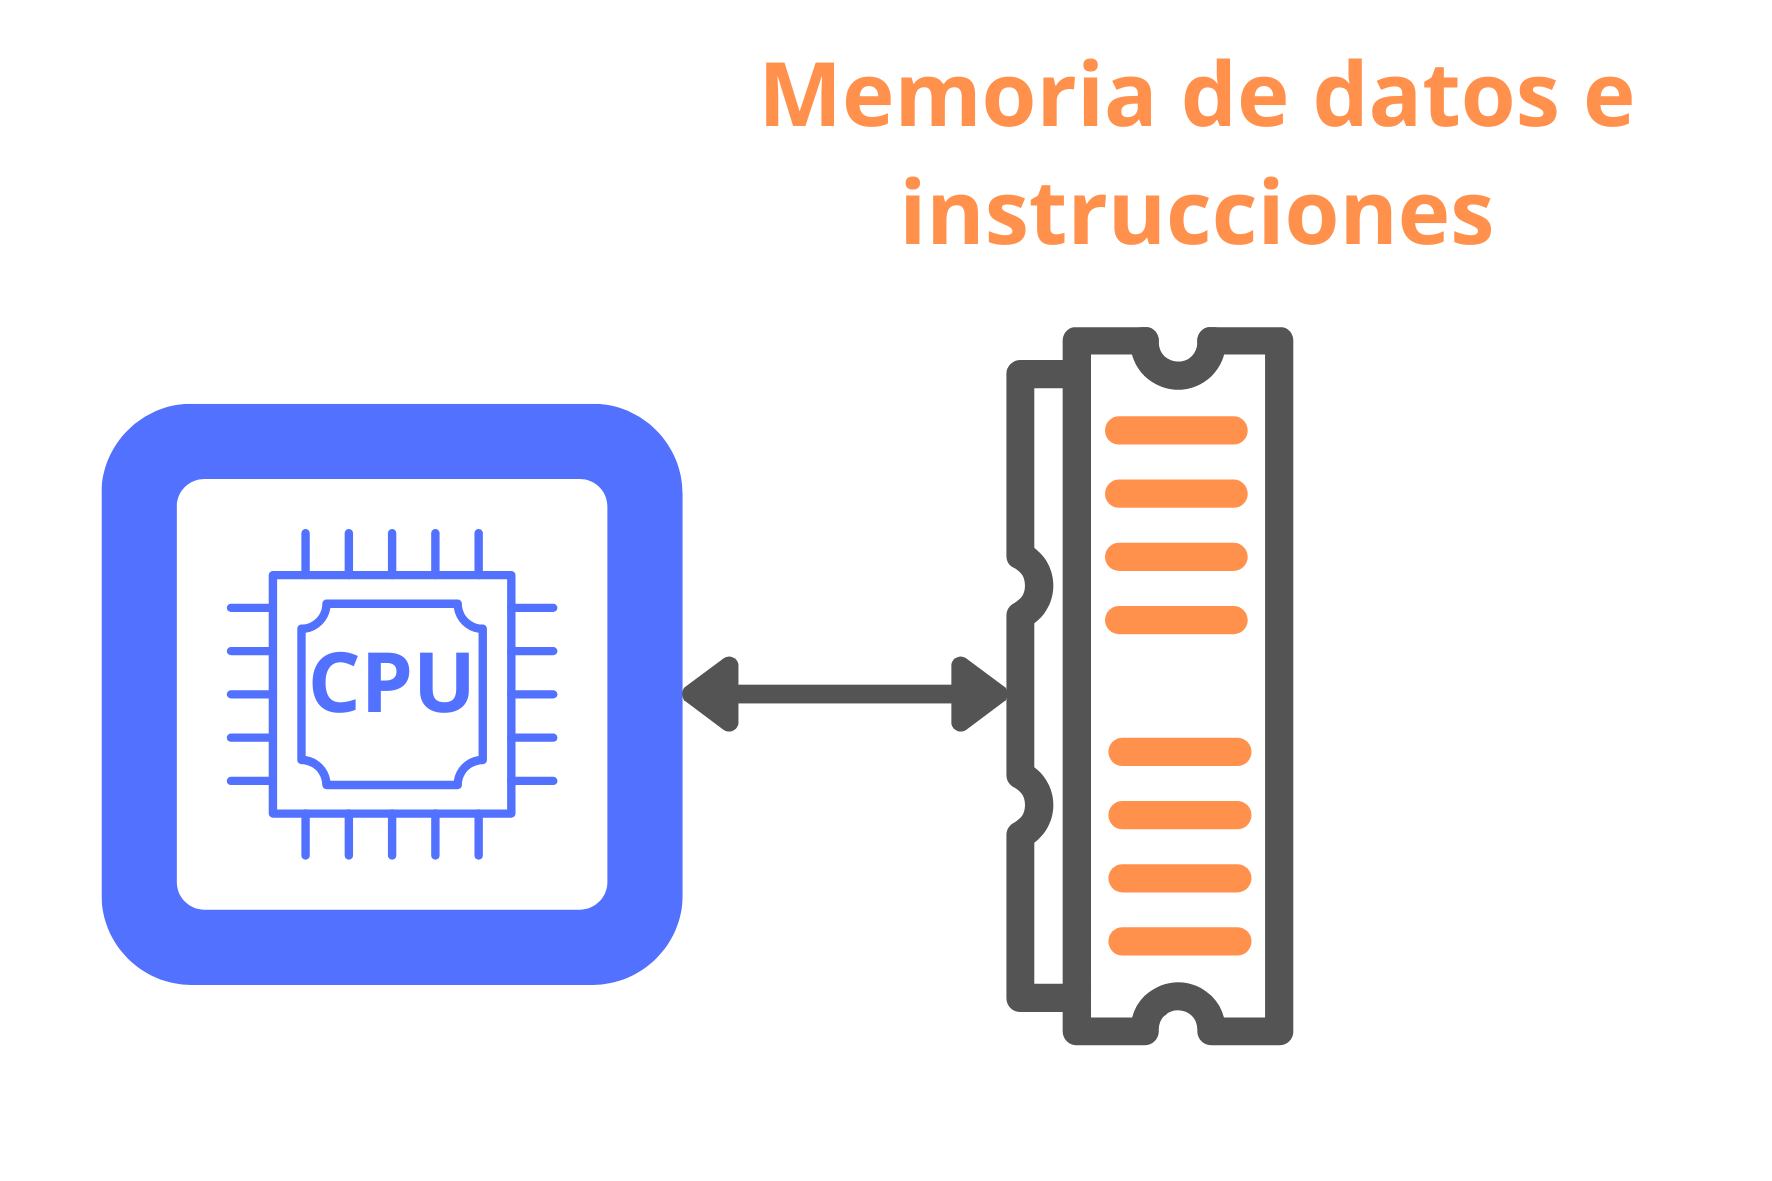
\includegraphics[width=0.85\linewidth]{images/vonneumann} 

}

\caption{Arquitectura Von Neumann}\label{fig:vonneumann}
\end{figure}

\hypertarget{arquitectura-harvard}{%
\subsection{Arquitectura Harvard}\label{arquitectura-harvard}}

Mientras la arquitectura Von Neumann se convertía en el paradigma dominante, paralelamente se desarrollaba un enfoque alternativo. La arquitectura Harvard tiene su origen en el diseño del Harvard Mark I, una computadora electromecánica desarrollada entre 1939 y 1944 durante la Segunda Guerra Mundial en la Universidad de Harvard bajo la dirección de Howard Aiken y con el apoyo de IBM \protect\hyperlink{ref-ceruzzi_history_2003}{{[}41{]}}, \protect\hyperlink{ref-williams1998history}{{[}42{]}}. El Harvard Mark I sentó las bases para un modelo arquitectónico diferente al de Von Neumann, caracterizado por una separación física entre instrucciones y datos.En este modelo, los datos y las instrucciones residen en memorias físicamente separadas, accedidas a través de buses independientes, lo cual mejora la eficiencia del procesamiento al eliminar la competencia por el bus entre instrucciones y datos. Esta organización evita el cuello de botella característico de Von Neumann y permite un acceso paralelo que incrementa el rendimiento en escenarios críticos para la eficiencia. A continuación, se presenta una comparación sistemática entre ambos modelos, a fin de comprender mejor sus implicancias técnicas y contextos de aplicación \protect\hyperlink{ref-tanenbaum_structured_2016}{{[}28{]}}. Debido a su eficiencia, esta arquitectura se ha adoptado ampliamente en sistemas embebidos, microcontroladores y procesadores de señal digital (DSP) \protect\hyperlink{ref-noergaard2012embedded}{{[}43{]}}.

\begin{figure}

{\centering 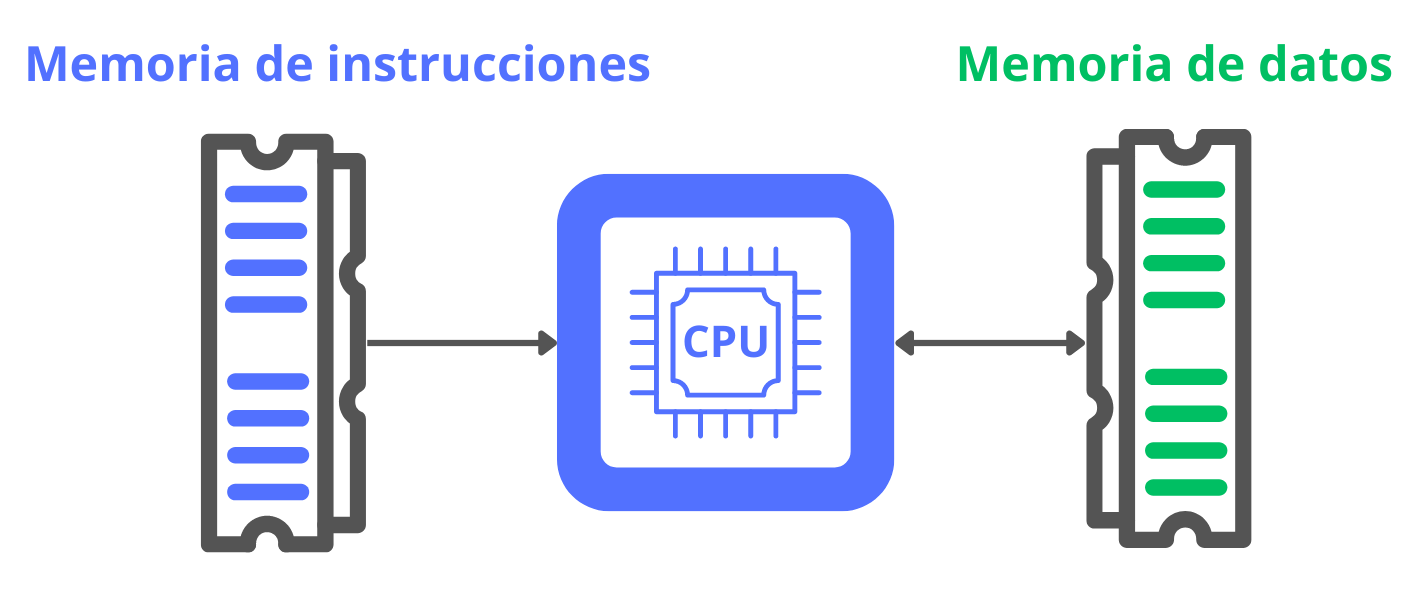
\includegraphics[width=0.85\linewidth]{images/harvard} 

}

\caption{Arquitectura Harvard}\label{fig:harvard}
\end{figure}

\hypertarget{comparativa-entre-von-neumann-y-harvard}{%
\subsection{Comparativa entre Von Neumann y Harvard}\label{comparativa-entre-von-neumann-y-harvard}}

Como señalan Stallings \protect\hyperlink{ref-stallings_computer_2021}{{[}20{]}} y Hennessy \protect\hyperlink{ref-hennessy2017computer}{{[}19{]}}, la arquitectura Von Neumann continúa siendo una alternativa predominante cuando se priorizan la simplicidad del diseño, la flexibilidad en la asignación de memoria y la compatibilidad con software de propósito general, como ocurre en muchas computadoras personales y servidores contemporáneos. En cambio, la arquitectura Harvard ha demostrado ventajas significativas en aplicaciones que demandan procesamiento en tiempo real y eficiencia energética, como dispositivos móviles, microcontroladores y entornos de control industrial. La elección entre ambas arquitecturas responde, en última instancia, a requerimientos específicos del sistema, ya sea por su complejidad, restricciones energéticas o necesidades de rendimiento paralelo.

Para una comparación más sistemática, se pueden establecer criterios como tipo de memoria, estructura de buses, capacidad de acceso paralelo, casos de uso representativos, ventajas y limitaciones.

\begin{table}[!h]
\centering
\caption{\label{tab:unnamed-chunk-1}Cuadro comparativo entre arquitecturas Von Neumann y Harvard}
\centering
\resizebox{\ifdim\width>\linewidth\linewidth\else\width\fi}{!}{
\fontsize{10}{12}\selectfont
\begin{tabular}[t]{>{\centering\arraybackslash}p{4cm}|>{\centering\arraybackslash}p{5.5cm}>{\centering\arraybackslash}p{5.5cm}}
\toprule
\multicolumn{1}{>{\centering\arraybackslash}p{4cm}}{\cellcolor[HTML]{D3D3D3}{\textbf{Característica}}} & \multicolumn{1}{>{\centering\arraybackslash}p{5.5cm}}{\cellcolor[HTML]{D3D3D3}{\textbf{Von Neumann}}} & \multicolumn{1}{>{\centering\arraybackslash}p{5.5cm}}{\cellcolor[HTML]{D3D3D3}{\textbf{Harvard}}}\\
\midrule
\textbf{Memoria} & Única para datos e instrucciones & Separada para datos e instrucciones\\
\addlinespace[10pt]
\textbf{Buses} & Bus compartido & Buses independientes\\
\addlinespace[10pt]
\textbf{Acceso simultáneo} & No & Sí\\
\addlinespace[10pt]
\textbf{Ejemplo típico} & Intel x86 & AVR, PIC\\
\addlinespace[10pt]
\textbf{Ventaja principal} & Diseño más simple & Mayor rendimiento\\
\addlinespace[10pt]
\addlinespace
\textbf{Limitación principal} & Cuello de botella & Diseño más complejo\\
\addlinespace[10pt]
\bottomrule
\end{tabular}}
\end{table}

Ambos modelos conceptuales han tenido una influencia decisiva en el diseño de arquitecturas contemporáneas. Mientras que el modelo Von Neumann ofrece un enfoque unificado que simplifica el desarrollo de software y hardware, la arquitectura Harvard destaca por su capacidad para mejorar el rendimiento mediante el acceso paralelo a instrucciones y datos. Esta distinción resulta crucial al analizar el diseño de arquitecturas modernas como x86, que constituye el foco de esta tesis. Comprender las implicancias de estas decisiones arquitectónicas es esencial para evaluar el impacto en el rendimiento, la eficiencia energética y la escalabilidad de los sistemas actuales.

El contraste entre estos dos modelos ha dado lugar a enfoques intermedios que buscan capitalizar las ventajas de ambos. Como resultado de esta evolución, emergen las denominadas arquitecturas híbridas, las cuales integran características de ambos modelos para optimizar el rendimiento y la flexibilidad del sistema.

\hypertarget{arquitecturas-huxedbridas}{%
\subsection{Arquitecturas híbridas}\label{arquitecturas-huxedbridas}}

Muchas arquitecturas contemporáneas implementan un enfoque híbrido, también conocido como arquitectura Harvard modificada. Este modelo emplea memorias separadas para datos e instrucciones a nivel microarquitectónico a menudo mediante la utilización de memorias caché de nivel 1 (L1) separadas para instrucciones y datos. No obstante, desde la perspectiva del programador, el modelo de memoria se mantiene unificado, facilitando el desarrollo de software sin exponer la complejidad del diseño interno. Esta dualidad permite optimizar la implementación física del procesador sin complicar el modelo de programación \protect\hyperlink{ref-hennessy2017computer}{{[}19{]}}, \protect\hyperlink{ref-stallings_computer_2021}{{[}20{]}}, \protect\hyperlink{ref-null_essentials_2023}{{[}33{]}}, \protect\hyperlink{ref-patterson_computer_2017}{{[}37{]}}.

\begin{figure}

{\centering 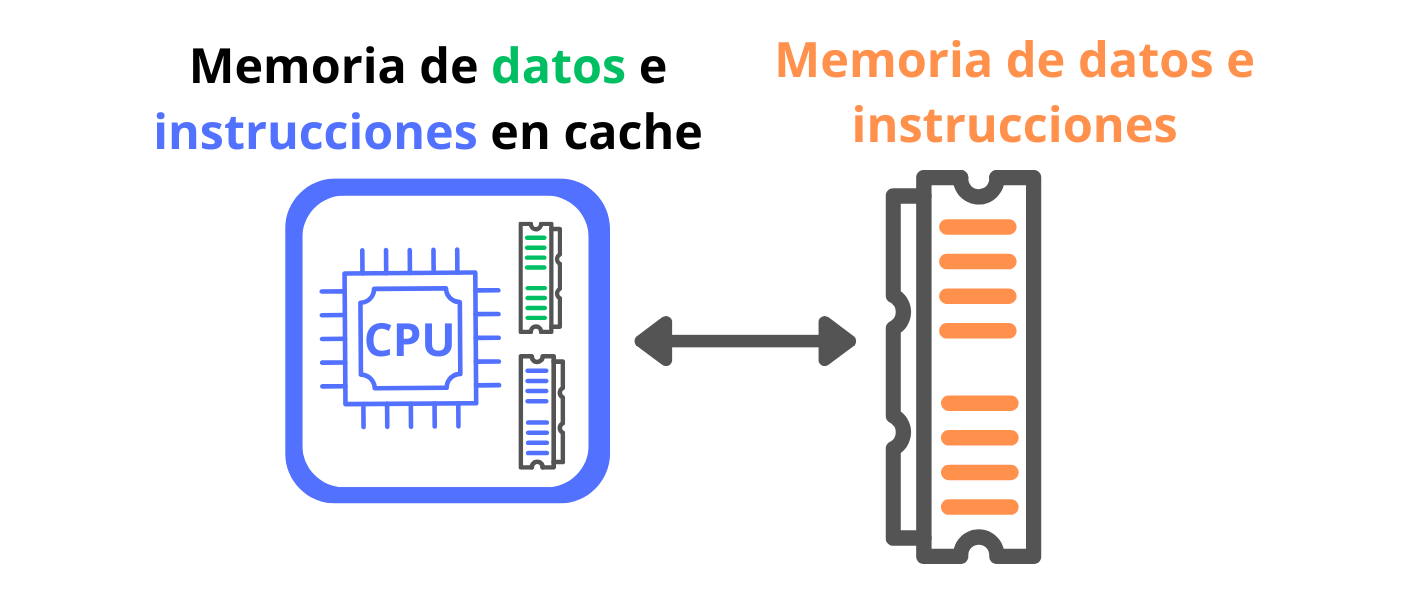
\includegraphics[width=0.85\linewidth]{images/hibrida} 

}

\caption{Arquitectura Híbridas}\label{fig:hibrida}
\end{figure}

Esta aproximación híbrida se implementa en arquitecturas modernas como ARM Cortex y los procesadores Intel Core, los cuales incorporan cachés separadas para instrucciones y datos con el objetivo de optimizar el rendimiento del pipeline, lo que facilita una mayor paralelización del procesamiento y reduce los conflictos en el acceso a memoria. A pesar de que el modelo de memoria visible para el programador se presenta como unificado, a nivel interno se implementan mecanismos característicos de la arquitectura Harvard, como el uso de memorias caché separadas para instrucciones y datos \protect\hyperlink{ref-arm2021architecture}{{[}44{]}}, \protect\hyperlink{ref-intel_microarchitecture_2021}{{[}45{]}}.

La adopción de arquitecturas híbridas, como la Harvard modificada, ha permitido a los diseñadores combinar la flexibilidad del modelo Von Neumann con la eficiencia del modelo Harvard. Esta convergencia no solo optimiza el rendimiento de los sistemas, sino que también responde a las exigencias contemporáneas en términos de consumo energético y capacidad de procesamiento paralelo. En este sentido, la distinción entre ambos modelos continúa siendo un eje conceptual clave para comprender la evolución de las arquitecturas modernas y su adaptación a diferentes escenarios tecnológicos.

En síntesis, la comprensión de las arquitecturas fundamentales ---Von Neumann, Harvard e híbridas--- resulta esencial para el desarrollo de herramientas de simulación efectivas en la enseñanza de arquitectura de computadoras. Los conceptos explorados en esta sección proporcionan los fundamentos conceptuales esenciales para el diseño y desarrollo de la herramienta de simulación propuesta en esta tesis.

\hypertarget{tipos-de-arquitecturas}{%
\section{Tipos de arquitecturas}\label{tipos-de-arquitecturas}}

El análisis de diversas arquitecturas de computadoras, y particularmente de sus repertorios de instrucciones (Instruction Set Architecture, ISA), es esencial para comprender sus ventajas, limitaciones y áreas de aplicación. Esta evaluación comparativa permite a los diseñadores y educadores seleccionar la ISA más adecuada para sus necesidades, considerando factores como la eficiencia energética, la complejidad del hardware, la compatibilidad y el soporte educativo.

Aunque arquitecturas como PowerPC, SPARC o MIPS desempeñaron un papel central en la evolución de la computación, su adopción ha disminuido significativamente en contextos industriales y académicos, debido al desplazamiento por plataformas con mayor soporte comercial y vigencia tecnológica \protect\hyperlink{ref-stallings_computer_2021}{{[}20{]}}. Su menor vigencia actual responde al surgimiento de arquitecturas más eficientes y con mejor respaldo comercial, como x86, ARM y RISC-V, que han captado la atención tanto del mercado como del ámbito educativo \protect\hyperlink{ref-waterman_risc-v_2014}{{[}31{]}}, \protect\hyperlink{ref-null_essentials_2023}{{[}33{]}}, \protect\hyperlink{ref-hennessy2017computer_riscv}{{[}46{]}}, \protect\hyperlink{ref-arm_evolution_2025}{{[}47{]}}. Por ello, esta sección se enfoca en aquellas arquitecturas que mantienen relevancia comercial o presentan un valor pedagógico significativo en el desarrollo de simuladores educativos.

\hypertarget{arquitectura-x86}{%
\subsection{Arquitectura x86}\label{arquitectura-x86}}

La arquitectura x86, desarrollada inicialmente por Intel, ha dominado el mercado de computadoras de escritorio y servidores durante décadas, gracias a su evolución constante y soporte del ecosistema de software \protect\hyperlink{ref-hennessy2017computer}{{[}19{]}}. Su conjunto de instrucciones (ISA, por sus siglas en inglés Instruction Set Architecture) incluye una amplia gama de operaciones, lo que otorga flexibilidad, aunque complica el diseño del hardware. Este equilibrio entre compatibilidad y rendimiento hace que x86 sea una opción preferida para entornos donde la capacidad de procesamiento es prioritaria, como en servidores y estaciones de trabajo \protect\hyperlink{ref-hennessy2017computer}{{[}19{]}}, \protect\hyperlink{ref-intel_whitepaper_2023}{{[}48{]}}.

\hypertarget{arquitectura-arm}{%
\subsection{Arquitectura ARM}\label{arquitectura-arm}}

Reconocida por su alta eficiencia energética, la arquitectura ARM es la columna vertebral de dispositivos móviles y sistemas embebidos. Basada en el paradigma de conjunto de instrucciones reducidas (RISC), ARM simplifica el diseño del hardware y optimiza el consumo energético, características que la posicionan como una opción preferente para aplicaciones como smartphones y tablets. Aunque su rendimiento máximo en tareas de cómputo intensivo suele ser inferior al de x86, su equilibrio entre eficiencia energética y capacidad computacional resulta decisivo en mercados donde la autonomía y la disipación térmica son factores críticos, como los dispositivos móviles y el IoT \protect\hyperlink{ref-patterson_computer_2014}{{[}34{]}}, \protect\hyperlink{ref-arm_evolution_2025}{{[}47{]}}.

\hypertarget{arquitectura-risc-v}{%
\subsection{Arquitectura RISC-V}\label{arquitectura-risc-v}}

Como arquitectura de código abierto, RISC-V ofrece una alternativa personalizable a los modelos propietarios, destacándose en entornos académicos y de desarrollo especializado. Su ISA flexible permite a los desarrolladores personalizar sistemas según necesidades específicas, haciéndola especialmente atractiva para investigación, educación y aplicaciones embebidas. Basada en principios RISC, RISC-V combina eficiencia energética con un diseño de hardware simplificado, y su creciente ecosistema la posiciona como una fuerte competidora frente a arquitecturas establecidas como ARM. No obstante, RISC-V enfrenta desafíos para su adopción masiva, en parte debido a la falta de estándares unificados, la fragmentación de su ecosistema y la limitada presencia de proveedores comerciales consolidados, lo que dificulta su despliegue en entornos productivos críticos.\protect\hyperlink{ref-waterman_risc-v_2014}{{[}31{]}}, \protect\hyperlink{ref-harris2015digital}{{[}32{]}}, \protect\hyperlink{ref-hennessy2017computer_riscv}{{[}46{]}}, \protect\hyperlink{ref-patterson2016computer}{{[}49{]}}.

\hypertarget{comparativa-entre-arquitecturas}{%
\subsection{Comparativa entre arquitecturas}\label{comparativa-entre-arquitecturas}}

Las características distintivas de cada arquitectura condicionan su idoneidad para diversas aplicaciones. Por ejemplo, mientras x86 sobresale en entornos de alto rendimiento, ARM domina en dispositivos móviles gracias a su eficiencia energética. Por su parte, arquitecturas como RISC-V han encontrado aplicaciones relevantes en sistemas embebidos, plataformas educativas y diseños personalizados, aunque su presencia comercial difiere notablemente. La selección adecuada de una arquitectura impacta significativamente en el éxito de un proyecto, desde el diseño hasta su implementación final. Además, comprender las diferencias entre estas arquitecturas, en particular sus repertorios de instrucciones y principios de diseño, resulta fundamental en el ámbito educativo, dado que facilita el desarrollo de herramientas didácticas que simulan sus principios operativos y ayudan a los estudiantes a visualizar el funcionamiento real de los sistemas computacionales \protect\hyperlink{ref-patterson_computer_2014}{{[}34{]}}, \protect\hyperlink{ref-arm_evolution_2025}{{[}47{]}}.

\begin{table}[!h]
\centering
\caption{\label{tab:aplicacionessimulacion}Aplicaciones de la simulación en distintos sectores}
\centering
\resizebox{\ifdim\width>\linewidth\linewidth\else\width\fi}{!}{
\fontsize{10}{12}\selectfont
\begin{tabular}[t]{>{\centering\arraybackslash}p{3cm}|>{\raggedright\arraybackslash}p{5cm}>{\raggedright\arraybackslash}p{6cm}}
\toprule
\multicolumn{1}{>{\centering\arraybackslash}p{3cm}}{\cellcolor[HTML]{D3D3D3}{\textbf{Sector}}} & \multicolumn{1}{>{\centering\arraybackslash}p{5cm}}{\cellcolor[HTML]{D3D3D3}{\textbf{Aplicación}}} & \multicolumn{1}{>{\centering\arraybackslash}p{6cm}}{\cellcolor[HTML]{D3D3D3}{\textbf{Beneficio principal}}}\\
\midrule
\textbf{Automotriz} & Pruebas de colisión virtuales & Reducción de costos y aumento de seguridad\\
\addlinespace[10pt]
\textbf{Aeroespacial} & Simuladores de vuelo & Entrenamiento sin riesgo\\
\addlinespace[10pt]
\textbf{Medicina} & Simulación de cirugías & Entrenamiento sin comprometer pacientes\\
\addlinespace[10pt]
\textbf{Educación} & Simuladores para arquitectura de computadoras & Comprensión de procesos abstractos\\
\addlinespace[10pt]
\bottomrule
\end{tabular}}
\end{table}

En el contexto de la enseñanza de arquitectura de computadoras, estas arquitecturas permiten abordar distintos niveles de complejidad y estilos de diseño, lo que resulta clave para la construcción de simuladores educativos efectivos.

\hypertarget{repertorio-de-instrucciones}{%
\section{Repertorio de instrucciones}\label{repertorio-de-instrucciones}}

El repertorio de instrucciones, o Instruction Set Architecture (ISA), es el conjunto de operaciones que un procesador puede ejecutar, incluyendo su representación binaria y el conjunto de reglas que definen la interacción entre el software y el hardware. El ISA define la interfaz entre el hardware y el software, abarcando instrucciones aritméticas, lógicas, de control y de manipulación de datos, así como los modos de direccionamiento y los formatos de instrucción. Por su influencia directa en el rendimiento, la eficiencia energética y la versatilidad del sistema, el ISA constituye un componente esencial en el diseño de arquitecturas de computadoras \protect\hyperlink{ref-hennessy2017computer}{{[}19{]}}, \protect\hyperlink{ref-stallings_computer_2021}{{[}20{]}}, \protect\hyperlink{ref-null_essentials_2023}{{[}33{]}}.

\hypertarget{caracteruxedsticas-clave-del-isa}{%
\subsection{Características clave del ISA}\label{caracteruxedsticas-clave-del-isa}}

Entre las características fundamentales a considerar en el diseño de un repertorio de instrucciones se encuentran las siguientes \protect\hyperlink{ref-hennessy2017computer}{{[}19{]}}:

\begin{itemize}
\tightlist
\item
  \textbf{Tipos de operandos}: representan los datos que las instrucciones pueden manipular, como enteros, números en punto flotante, caracteres y direcciones de memoria. Un ISA eficiente debe soportar una amplia variedad de operandos para maximizar su versatilidad.
\item
  \textbf{Tipos de operaciones}: incluyen las operaciones que el procesador puede realizar, como aritméticas (suma, resta), lógicas (AND, OR), de control (saltos, llamadas a subrutinas) y de manipulación de datos (almacenamiento, carga). Diversos autores destacan que un ISA bien diseñado debe lograr un equilibrio entre funcionalidad, simplicidad y eficiencia de implementación, aspectos fundamentales en el diseño de arquitecturas modernas \protect\hyperlink{ref-hennessy2017computer}{{[}19{]}}, \protect\hyperlink{ref-null_essentials_2023}{{[}33{]}}.
\item
  \textbf{Modos de direccionamiento}: determinan cómo se especifican los operandos en las instrucciones. Entre los modos más comunes se encuentran el inmediato, directo, indirecto, mediante registros, con desplazamiento y basado en pila. Cada uno ofrece distintos niveles de eficiencia, flexibilidad y complejidad, siendo fundamentales para optimizar el acceso a datos y la ejecución de instrucciones.
\item
  \textbf{Formato de las instrucciones}: que definen las reglas para acceder a los operandos dentro de las instrucciones, se exploran con mayor detalle en la siguiente subsección.
\end{itemize}

\begin{figure}

{\centering 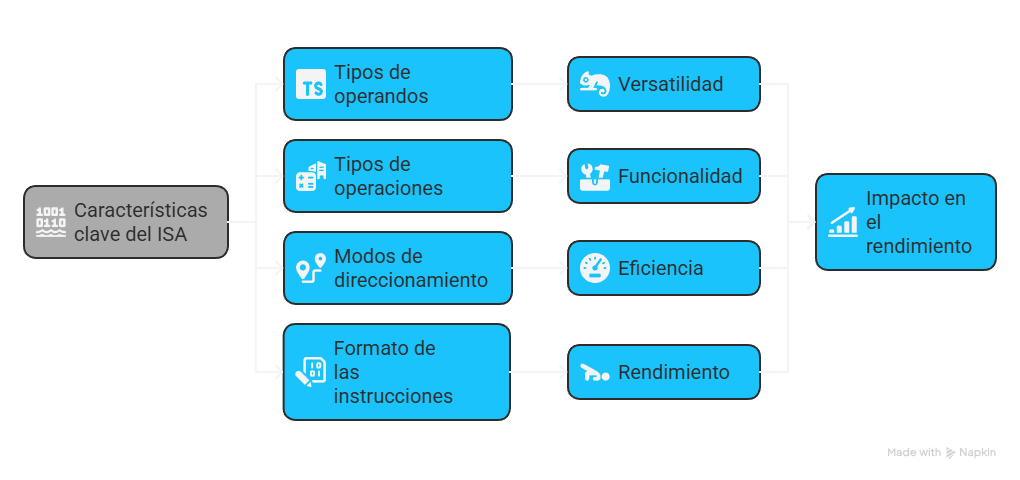
\includegraphics[width=1\linewidth]{images/isa} 

}

\caption{Características repertorio de instrucciones}\label{fig:repInstCaracteristicas}
\end{figure}

El diseño de un repertorio de instrucciones eficiente y versátil es un desafío complejo que requiere un equilibrio entre funcionalidad, rendimiento y facilidad de uso. La selección adecuada de operandos, operaciones y modos de direccionamiento, junto con un formato de instrucción bien estructurado, son aspectos fundamentales para lograr una arquitectura de computadoras efectiva y adaptable a diversas aplicaciones. Estas características no solo definen las capacidades funcionales de un procesador, sino que también condicionan la manera en que las instrucciones interactúan con la memoria y los registros. A continuación, se profundiza en los modos de direccionamiento, uno de los elementos que más influye en la flexibilidad y eficiencia del repertorio de instrucciones.

\hypertarget{modos-de-direccionamiento}{%
\subsection{Modos de direccionamiento}\label{modos-de-direccionamiento}}

Los modos de direccionamiento definen los mecanismos mediante los cuales una instrucción especifica la ubicación de sus operandos, permitiendo así al procesador acceder a los datos en memoria o registros en tiempo de ejecución. A continuación, se describen los modos de direccionamiento más comúnmente implementados en las arquitecturas modernas \protect\hyperlink{ref-hennessy2017computer}{{[}19{]}}, \protect\hyperlink{ref-stallings_computer_2021}{{[}20{]}}:

\begin{enumerate}
\def\labelenumi{\alph{enumi})}
\tightlist
\item
  \textbf{Inmediato}: el operando está directamente incluido en la instrucción, permitiendo acceso rápido a valores constantes. Es eficiente para operaciones simples, aunque limitado a operandos pequeños.
\item
  \textbf{Directo}: la instrucción contiene la dirección de memoria del operando. Es fácil de usar, pero está restringido por el rango de direcciones accesibles.
\item
  \textbf{Indirecto}: la instrucción apunta a una dirección que contiene la ubicación real del operando, lo que amplía el rango de direcciones a costa de un acceso adicional a memoria.
\item
  \textbf{Registro}: el operando se encuentra en un registro del procesador, proporcionando acceso extremadamente rápido, pero limitado por la cantidad de registros disponibles.
\item
  \textbf{Registro Indirecto}: similar al modo indirecto, pero la dirección efectiva se obtiene a partir del contenido de un registro, lo que ofrece un buen equilibrio entre velocidad de acceso y capacidad de direccionamiento.
\item
  \textbf{Con Desplazamiento}: combina una dirección base con un valor de desplazamiento, ideal para estructuras como arrays y matrices.
\item
  \textbf{Pila}: el operando está en la parte superior de la pila, útil para gestionar subrutinas y el paso de parámetros.
\end{enumerate}

Para complementar la descripción anterior, la Figura \ref{fig:ModDir} presenta una representación esquemática de los modos de direccionamiento, mostrando gráficamente cómo se calcula la dirección efectiva (EA) en cada caso \protect\hyperlink{ref-stallings_computer_2021}{{[}20{]}}.

\begin{figure}

{\centering 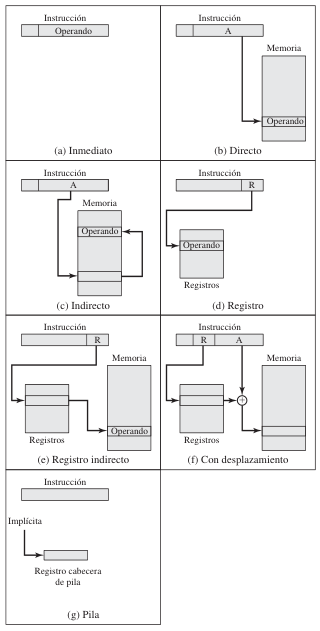
\includegraphics[width=0.6\linewidth]{images/modosdireccionamiento} 

}

\caption{Modos de direccionamiento }\label{fig:ModDir}
\end{figure}

\begin{itemize}
\tightlist
\item
  A = contenido de un campo de dirección en la instrucción
\item
  R = contenido de un campo de dirección en la instrucción que referencia a un registro
\item
  EA = dirección real (efectiva) de la posición que contiene el operando que se referencia
\end{itemize}

La tabla \ref{tab:tabmoddir} detalla el cálculo de la dirección para cada modo de direccionamiento.

\begin{table}[!h]
\centering
\caption{\label{tab:tabmoddir}Modos de direccionamiento básicos}
\centering
\resizebox{\ifdim\width>\linewidth\linewidth\else\width\fi}{!}{
\fontsize{10}{12}\selectfont
\begin{tabular}[t]{>{\raggedright\arraybackslash}p{4cm}|>{\raggedright\arraybackslash}p{4cm}>{\raggedright\arraybackslash}p{4cm}>{\raggedright\arraybackslash}p{4cm}}
\toprule
\multicolumn{1}{>{\centering\arraybackslash}p{4cm}}{\cellcolor[HTML]{D3D3D3}{\textbf{Modo}}} & \multicolumn{1}{>{\centering\arraybackslash}p{4cm}}{\cellcolor[HTML]{D3D3D3}{\textbf{Algoritmo}}} & \multicolumn{1}{>{\centering\arraybackslash}p{4cm}}{\cellcolor[HTML]{D3D3D3}{\textbf{Ventaja}}} & \multicolumn{1}{>{\centering\arraybackslash}p{4cm}}{\cellcolor[HTML]{D3D3D3}{\textbf{Desventaja}}}\\
\midrule
\textbf{Inmediato} & Operando ← A & No referencia a memoria & Operando de magnitud limitada\\
\addlinespace[10pt]
\textbf{Directo} & EA ← A & Es sencillo & Espacio de direcciones limitado\\
\addlinespace[10pt]
\textbf{Indirecto} & EA ← (A) & Espacio de direcciones grande & Referencias múltiples a memoria\\
\addlinespace[10pt]
\textbf{Registro} & EA ← R & No referencia a memoria & Número limitado de registros\\
\addlinespace[10pt]
\textbf{Indirecto con registro} & EA ← (R) & Espacio de direcciones grande & Referencia extra a memoria\\
\addlinespace[10pt]
\addlinespace
\textbf{Con desplazamiento} & EA ← A + (R) & Flexibilidad & Complejidad\\
\addlinespace[10pt]
\textbf{Pila} & EA ← puntero de pila & No referencia a memoria & Aplicabilidad limitada\\
\addlinespace[10pt]
\bottomrule
\end{tabular}}
\end{table}

\hypertarget{formato-de-las-instrucciones}{%
\subsection{Formato de las instrucciones}\label{formato-de-las-instrucciones}}

El formato de las instrucciones especifica la disposición y codificación de los elementos que conforman una instrucción, como el código de operación (opcode), los operandos, los modos de direccionamiento y otros campos auxiliares. Esta organización impacta directamente en la facilidad de decodificación y en el rendimiento del procesador. Este formato afecta la rapidez de decodificación y la eficiencia general del procesador \protect\hyperlink{ref-hennessy2017computer}{{[}19{]}}, \protect\hyperlink{ref-tanenbaum_structured_2016}{{[}28{]}}:

\begin{itemize}
\tightlist
\item
  \textbf{Longitud de la instrucción}: puede ser fija o variable. Las instrucciones de longitud fija permiten una decodificación más rápida y simplifican la lógica de control del procesador. En cambio, las instrucciones de longitud variable permiten una codificación más eficiente del espacio de memoria, a costa de una mayor complejidad en la etapa de decodificación.
\item
  \textbf{Cantidad de operandos}: las instrucciones pueden trabajar con diferentes números de operandos (de 0 a 3 o más). Una mayor cantidad de operandos incrementa la expresividad de las instrucciones, pero también puede derivar en una mayor complejidad de codificación y en un mayor uso de recursos del procesador.
\item
  \textbf{Campos de instrucción}: incluyen el opcode y campos adicionales como operandos, modos de direccionamiento y flags de condición. Estos campos determinan cuántas y qué tipo de operaciones puede ejecutar el procesador en un ciclo de reloj.
\end{itemize}

La Figura \ref{fig:forminst} muestra un ejemplo representativo de formato de instrucción, donde se visualizan los campos que la componen y su disposición en el código binario.

\begin{figure}

{\centering 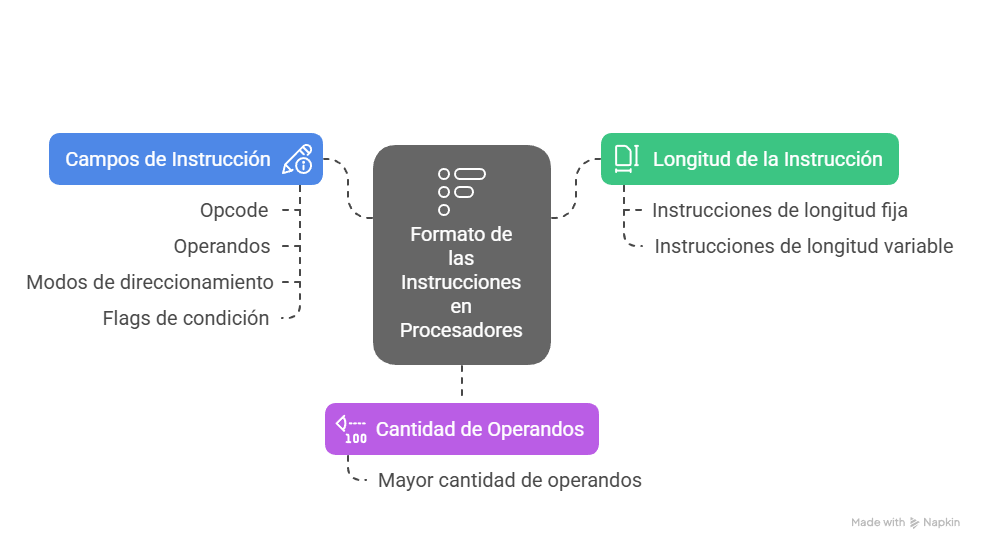
\includegraphics[width=1\linewidth]{images/formatoinst} 

}

\caption{Formato de instrucciones }\label{fig:forminst}
\end{figure}

\hypertarget{comparativa-de-repertorios-de-instrucciones}{%
\subsection{Comparativa de repertorios de instrucciones}\label{comparativa-de-repertorios-de-instrucciones}}

La siguiente tabla \ref{tab:comparativaISA} resume las características principales de los repertorios de instrucciones en tres arquitecturas ampliamente utilizadas: x86, ARM y RISC-V. Se consideran aspectos como la longitud de las instrucciones, la cantidad de operandos, su complejidad y los modos de direccionamiento que permiten.

\begin{table}[!h]
\centering
\caption{\label{tab:comparativaISA}Comparativa de repertorios de instrucciones reales}
\centering
\resizebox{\ifdim\width>\linewidth\linewidth\else\width\fi}{!}{
\fontsize{10}{12}\selectfont
\begin{tabular}[t]{>{\centering\arraybackslash}p{3cm}|>{\centering\arraybackslash}p{4cm}>{\centering\arraybackslash}p{4cm}>{\centering\arraybackslash}p{4cm}>{\centering\arraybackslash}p{4cm}}
\toprule
\multicolumn{1}{>{\centering\arraybackslash}p{3cm}}{\cellcolor[HTML]{D3D3D3}{\textbf{Arquitectura}}} & \multicolumn{1}{>{\centering\arraybackslash}p{4cm}}{\cellcolor[HTML]{D3D3D3}{\textbf{Longitud instrucción}}} & \multicolumn{1}{>{\centering\arraybackslash}p{4cm}}{\cellcolor[HTML]{D3D3D3}{\textbf{Nº operandos}}} & \multicolumn{1}{>{\centering\arraybackslash}p{4cm}}{\cellcolor[HTML]{D3D3D3}{\textbf{Tipos de operandos}}} & \multicolumn{1}{>{\centering\arraybackslash}p{4cm}}{\cellcolor[HTML]{D3D3D3}{\textbf{Modos de direccionamiento}}}\\
\midrule
\textbf{x86} & Variable & 0–3+ & Complejos & Muchos\\
\addlinespace[10pt]
\textbf{ARM} & Fija (32 bits) & 3 & Simples & Limitados\\
\addlinespace[10pt]
\textbf{RISC-V} & Fija (32 bits) & 3 & Simples & Extensible\\
\addlinespace[10pt]
\bottomrule
\end{tabular}}
\end{table}

\hypertarget{filosofuxedas-cisc-y-risc}{%
\section{Filosofías CISC y RISC}\label{filosofuxedas-cisc-y-risc}}

El diseño del repertorio de instrucciones es una decisión estratégica clave en la arquitectura de procesadores, ya que determina no solo el rendimiento del sistema, sino también la complejidad del hardware y del software, en particular del compilador. Dos de las filosofías más influyentes en este campo son \textbf{CISC (Complex Instruction Set Computing)} y \textbf{RISC (Reduced Instruction Set Computing)}. Mientras que \textbf{CISC} prioriza la reducción del número de instrucciones necesarias para realizar tareas complejas mediante operaciones multifuncionales, \textbf{RISC} simplifica el conjunto de instrucciones con el objetivo de maximizar la velocidad y la eficiencia energética. En esta sección se analizan ambos enfoques y sus implicaciones en el diseño de procesadores \protect\hyperlink{ref-hennessy2017computer}{{[}19{]}}, \protect\hyperlink{ref-patterson_computer_2014}{{[}34{]}}.

El debate entre las filosofías CISC y RISC se remonta a fines de la década de 1970, cuando se comenzaron a cuestionar los beneficios reales de los repertorios de instrucciones complejos. Mientras las primeras generaciones de computadoras buscaban reducir el número de instrucciones por programa, investigaciones posteriores demostraron que un conjunto reducido y eficiente de instrucciones podía mejorar significativamente el rendimiento al simplificar la ejecución y optimizar el uso del hardware.

La evolución de los procesadores ha llevado a un enfoque más equilibrado, donde las arquitecturas modernas combinan elementos de ambas filosofías. Las arquitecturas modernas tienden a incorporar elementos de ambas filosofías. Por ejemplo, x86 adopta técnicas de ejecución interna propias de RISC para aumentar su rendimiento, mientras que procesadores RISC como ARM han introducido extensiones complejas para tareas específicas, acercándose parcialmente al enfoque CISC \protect\hyperlink{ref-hennessy2017computer}{{[}19{]}}, \protect\hyperlink{ref-patterson_computer_2014}{{[}34{]}}.

\hypertarget{cisc}{%
\subsection{CISC}\label{cisc}}

Las arquitecturas \textbf{CISC}, como la \textbf{x86}, se caracterizan por su enfoque en reducir el número de instrucciones requeridas para completar operaciones complejas. Esto se logra mediante la inclusión de instrucciones que combinan múltiples operaciones en un solo ciclo. Como resultado, los programadores necesitan escribir menos líneas de código para alcanzar un objetivo específico.

Sin embargo, este diseño implica ciertas desventajas. La \textbf{decodificación} y \textbf{ejecución} de instrucciones CISC requiere un hardware considerablemente más complejo, y las instrucciones de longitud variable, típicas de estas arquitecturas, pueden aumentar el tiempo de decodificación. Esto genera cuellos de botella en el pipeline y limita el rendimiento.

Un ejemplo representativo es la arquitectura x86, que ha incorporado técnicas internas de ejecución similares a RISC ---como la descomposición de instrucciones mediante microcódigo--- con el fin de mejorar el rendimiento sin abandonar su repertorio complejo. Utiliza microcódigo para descomponer las instrucciones complejas en operaciones más simples, parecidas a las de un procesador RISC. Aunque esta estrategia mejora la eficiencia de ejecución en algunos casos, el diseño sigue siendo más costoso en términos de consumo energético y complejidad \protect\hyperlink{ref-patterson_computer_2014}{{[}34{]}}.

En consecuencia, el diseño del repertorio de instrucciones ---incluyendo operaciones, modos de direccionamiento y formatos--- constituye la interfaz crítica entre hardware y software, afectando tanto la eficiencia de ejecución como la expresividad de los programas. Su diseño influye directamente en la eficiencia del procesamiento y en la forma en que los programas interactúan con la arquitectura subyacente, lo que refuerza su relevancia en el estudio de la arquitectura de computadoras.

\hypertarget{RISC}{%
\subsection{RISC}\label{RISC}}

Las arquitecturas basadas en RISC, en contraste con CISC, se caracterizan por emplear instrucciones simples y de longitud fija. Esta simplificación facilita la decodificación y permite que muchas instrucciones se ejecuten en un solo ciclo de reloj. Además, esta filosofía favorece la implementación de técnicas avanzadas como el pipelining y la predicción de ramas, optimizando así el rendimiento.

A nivel de hardware, RISC prioriza la eficiencia energética, una característica crucial en dispositivos móviles y sistemas embebidos. Por ello, procesadores como los basados en ARM han dominado estos mercados, especialmente en dispositivos móviles, debido a su bajo consumo energético. La simplicidad y el bajo CPI (ciclos por instrucción) han sido factores determinantes en su adopción \protect\hyperlink{ref-hennessy2017computer_riscv}{{[}46{]}}.

\hypertarget{comparativa-entre-cisc-y-risc}{%
\subsection{Comparativa entre CISC y RISC}\label{comparativa-entre-cisc-y-risc}}

Las diferencias entre CISC y RISC son evidentes tanto a nivel de diseño como de implementación. En las arquitecturas RISC, las instrucciones tienen una longitud fija, lo que simplifica la decodificación, reduce la latencia y mejora la predictibilidad del rendimiento. Además, este formato mejora la eficiencia del uso de la memoria caché, al ocupar menos espacio y facilitar accesos más rápidos.

En cambio, las arquitecturas CISC, como x86, emplean instrucciones de longitud variable, lo que les permite ofrecer una mayor flexibilidad y un repertorio más amplio de operaciones. Sin embargo, esta flexibilidad conlleva un mayor tiempo de decodificación y una complejidad adicional en la implementación del pipeline. Esto puede causar problemas como interrupciones en el flujo debido a errores de predicción de ramas, aunque se mitiguen mediante técnicas avanzadas como la predicción dinámica de saltos y el prefetching \protect\hyperlink{ref-tanenbaum_structured_2016}{{[}28{]}}.

Por ejemplo, en RISC, los modos de direccionamiento son simples y permiten un acceso más rápido a los operandos, reduciendo la latencia en el pipeline \protect\hyperlink{ref-stallings_computer_2021}{{[}20{]}}. En CISC, los modos de direccionamiento más complejos proporcionan flexibilidad a costa de una mayor latencia, lo que impacta negativamente en el rendimiento general del sistema.

\hypertarget{ejemplos-de-instrucciones}{%
\subsubsection{Ejemplos de instrucciones}\label{ejemplos-de-instrucciones}}

Para ilustrar la diferencia entre ambas filosofías, se presenta el siguiente ejemplo: cargar dos valores de memoria, sumarlos y almacenar el resultado en una dirección de memoria.

Una arquitectura bajo la filosofia RISC es RISC-V, que utiliza instrucciones simples y de longitud fija. En este caso, la instrucción para cargar un valor de memoria en un registro es \texttt{lw} (load word), y la instrucción para almacenar el resultado es \texttt{sw} (store word). La suma se realiza con la instrucción \texttt{add}.:

\begin{lstlisting}
    # Cargar el valor de mem1 en el registro t0 (R1)
    lw t0, 0(mem1)      # t0 = MEM[mem1]

    # Cargar el valor de mem2 en el registro t1 (R2)
    lw t1, 0(mem2)      # t1 = MEM[mem2]

    # Sumar los registros t0 y t1, guardar el resultado en t2 (R3)
    add t2, t0, t1      # t2 = t0 + t1

    # Guardar el resultado en mem1
    sw t2, 0(mem1)      # MEM[mem1] = t2
  \end{lstlisting}

Una arquitectura bajo la filosofia CISC es x86, que utiliza instrucciones más complejas y de longitud variable. En este caso, la instrucción para cargar un valor de memoria en un registro es \texttt{MOV}, y la instrucción para almacenar el resultado es también \texttt{MOV}. La suma se realiza con la instrucción \texttt{ADD}:

\begin{lstlisting}
  ; Cargar el valor almacenado en mem1 en el registro EAX
  MOV EAX, [mem1]

  ; Sumar el valor almacenado en mem2 al registro EAX
  ADD EAX, [mem2]

  ; Guardar el resultado de la suma de vuelta en mem1
  MOV [mem1], EAX
  \end{lstlisting}

La tabla \ref{tab:ciscrisc} sintetiza las principales diferencias estructurales y operativas entre las filosofías CISC y RISC, destacando sus implicancias en el diseño del hardware y el rendimiento general del sistema.

\begin{table}[!h]
\centering
\caption{\label{tab:ciscrisc}Comparativa entre CISC y RISC}
\centering
\resizebox{\ifdim\width>\linewidth\linewidth\else\width\fi}{!}{
\fontsize{10}{12}\selectfont
\begin{tabular}[t]{>{\raggedright\arraybackslash}p{4cm}|>{\raggedright\arraybackslash}p{5cm}>{\raggedright\arraybackslash}p{5cm}}
\toprule
\multicolumn{1}{>{\centering\arraybackslash}p{4cm}}{\cellcolor[HTML]{D3D3D3}{\textbf{Aspecto}}} & \multicolumn{1}{>{\centering\arraybackslash}p{5cm}}{\cellcolor[HTML]{D3D3D3}{\textbf{CISC}}} & \multicolumn{1}{>{\centering\arraybackslash}p{5cm}}{\cellcolor[HTML]{D3D3D3}{\textbf{RISC}}}\\
\midrule
\textbf{Objetivo principal} & Minimizar el número de instrucciones para operaciones complejas & Simplificar el conjunto de instrucciones para optimizar velocidad y eficiencia energética\\
\addlinespace[10pt]
\textbf{Tipo de instrucciones} & Instrucciones complejas, longitud variable & Instrucciones simples, longitud fija\\
\addlinespace[10pt]
\textbf{Decodificación y ejecución} & Requiere hardware más complejo, posibles cuellos de botella en el pipeline & Decodificación más sencilla, facilita el uso de técnicas avanzadas como pipelining\\
\addlinespace[10pt]
\textbf{Longitud de instrucciones} & Longitud variable, puede aumentar el tiempo de decodificación & Longitud fija, simplifica la decodificación y mejora la predictibilidad del rendimiento\\
\addlinespace[10pt]
\textbf{Eficiencia energética} & Menor eficiencia energética en comparación con RISC & Mayor eficiencia energética, especialmente en dispositivos móviles\\
\addlinespace[10pt]
\addlinespace
\textbf{Modos de direccionamiento} & Flexibilidad a costa de mayor latencia & Acceso más rápido a los operandos, menor latencia\\
\addlinespace[10pt]
\bottomrule
\end{tabular}}
\end{table}

\hypertarget{convergencia-de-filosofuxedas}{%
\subsubsection{Convergencia de filosofías}\label{convergencia-de-filosofuxedas}}

A pesar de sus diferencias, las arquitecturas modernas tienden a integrar características de ambas filosofías. Por ejemplo, los procesadores x86 adoptan técnicas propias de RISC para mejorar la eficiencia energética y el rendimiento. Esta convergencia refleja cómo los avances en diseño de procesadores buscan combinar lo mejor de cada enfoque, maximizando la flexibilidad y la eficiencia para adaptarse a las necesidades actuales y futuras del mercado.

La Figura \ref{fig:convergen} muestras la convergencia entre estas dos filosofías:

\begin{figure}

{\centering 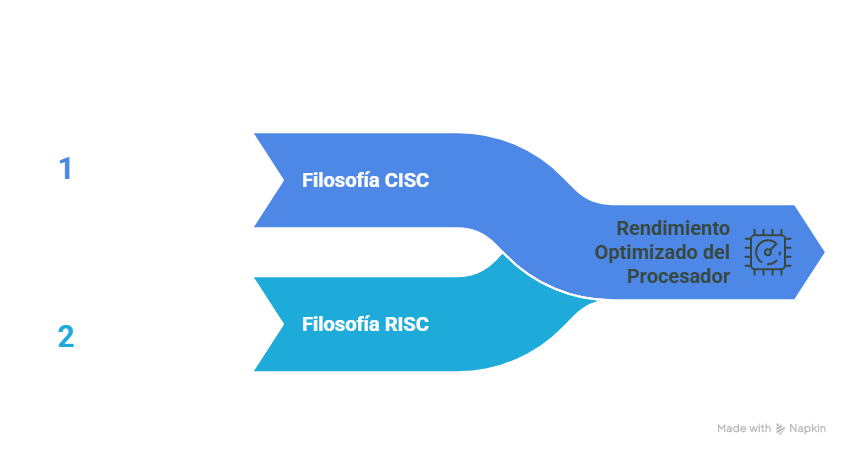
\includegraphics[width=1\linewidth]{images/convergen} 

}

\caption{Convergencia de filosofías}\label{fig:convergen}
\end{figure}

En síntesis, las filosofías CISC y RISC representan enfoques contrastantes pero complementarios en el diseño de arquitecturas de procesadores. Su comprensión no solo es esencial para analizar el rendimiento y la eficiencia energética de los sistemas modernos, sino también para formar una base sólida en la enseñanza de arquitectura de computadoras, especialmente en contextos donde se emplean simuladores didácticos.

\hypertarget{arquitectura-x86-1}{%
\section{Arquitectura x86}\label{arquitectura-x86-1}}

La arquitectura x86, reconocida por su amplia adopción en computadoras personales, estaciones de trabajo y servidores, se introdujo en 1978 con el procesador Intel 8086, basado en una arquitectura de 16 bits. Desde entonces, ha evolucionado en capacidad y complejidad, con hitos clave como la introducción del Intel 80386 (32 bits) en 1985 y la extensión a 64 bits con AMD64 en 2003. Esta evolución ha permitido mejoras significativas en el rendimiento, el direccionamiento de memoria y la compatibilidad con aplicaciones exigentes. \protect\hyperlink{ref-stallings_computer_2021}{{[}20{]}}, \protect\hyperlink{ref-intel_64_2025}{{[}21{]}}, \protect\hyperlink{ref-amd_developer_2024}{{[}22{]}}, \protect\hyperlink{ref-abel_ibm_2000}{{[}23{]}}, \protect\hyperlink{ref-brey_intel_microprocessors}{{[}50{]}}, \protect\hyperlink{ref-intel8086manual}{{[}51{]}}.

\begin{figure}

{\centering 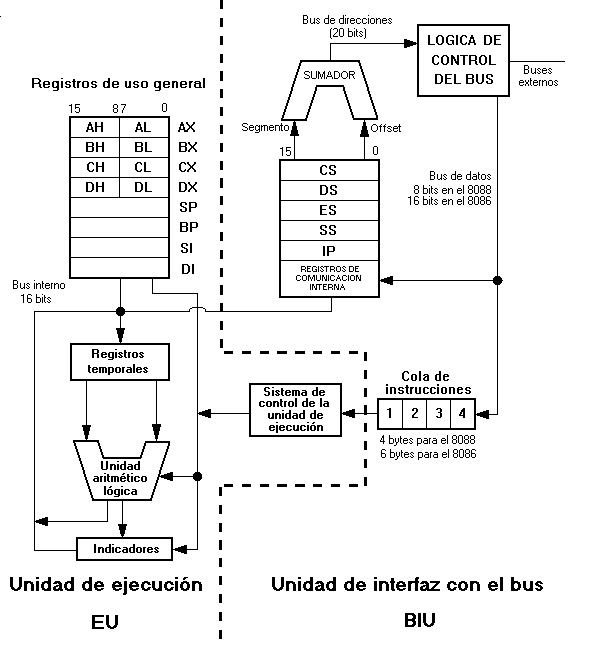
\includegraphics[width=1\linewidth]{images/x86} 

}

\caption{Diagrama esquemático microprocesador Intel 8086}\label{fig:x86}
\end{figure}

\hypertarget{evoluciuxf3n-de-la-arquitectura-x86}{%
\subsection{Evolución de la arquitectura x86}\label{evoluciuxf3n-de-la-arquitectura-x86}}

Uno de los pilares del éxito de la arquitectura x86 ha sido su retrocompatibilidad, permitiendo la ejecución de aplicaciones de 16, 32 y 64 bits en un mismo sistema. Dicha propiedad no solo ha garantizado la continuidad del ecosistema x86, sino que también ha protegido las inversiones en software y sistemas operativos, una característica fundamental en entornos empresariales y académicos.

A continuación, se presenta la tabla \ref{tab:hitosx86} que resume los hitos clave en la evolución de los procesadores x86:

\begin{table}[!h]
\centering
\caption{\label{tab:hitosx86}Hitos en la evolución x86}
\centering
\resizebox{\ifdim\width>\linewidth\linewidth\else\width\fi}{!}{
\fontsize{10}{12}\selectfont
\begin{tabular}[t]{>{\centering\arraybackslash}p{4cm}>{\centering\arraybackslash}p{4cm}>{\centering\arraybackslash}p{4cm}>{\raggedright\arraybackslash}p{4cm}}
\toprule
\multicolumn{1}{>{\centering\arraybackslash}p{4cm}}{\cellcolor[HTML]{D3D3D3}{\textbf{Procesador}}} & \multicolumn{1}{>{\centering\arraybackslash}p{4cm}}{\cellcolor[HTML]{D3D3D3}{\textbf{Año de Lanzamiento}}} & \multicolumn{1}{>{\centering\arraybackslash}p{4cm}}{\cellcolor[HTML]{D3D3D3}{\textbf{Número de Bits}}} & \multicolumn{1}{>{\centering\arraybackslash}p{4cm}}{\cellcolor[HTML]{D3D3D3}{\textbf{Extensiones de 64 bits}}}\\
\midrule
\textbf{Intel 8086} & 1978 & 16 & Arquitectura inicial\\
\addlinespace[10pt]
\textbf{Intel 80386} & 1985 & 32 & Memoria virtual\\
\addlinespace[10pt]
\textbf{AMD64} & 2003 & 64 & Extensiones de 64 bits\\
\addlinespace[10pt]
\bottomrule
\end{tabular}}
\end{table}

La tabla \ref{tab:evolucionx86} muestra cómo la evolución de x86 ha estado marcada por avances tecnológicos que han impulsado la informática hacia nuevas fronteras:

\begin{table}[!h]
\centering
\caption{\label{tab:evolucionx86}Línea de Tiempo de la Evolución de la Arquitectura x86}
\centering
\resizebox{\ifdim\width>\linewidth\linewidth\else\width\fi}{!}{
\fontsize{10}{12}\selectfont
\begin{tabular}[t]{>{\centering\arraybackslash}p{2cm}|>{\centering\arraybackslash}p{3.5cm}|>{\raggedright\arraybackslash}p{9cm}}
\toprule
\multicolumn{1}{>{\centering\arraybackslash}p{2cm}}{\cellcolor[HTML]{D3D3D3}{\textbf{Año}}} & \multicolumn{1}{>{\centering\arraybackslash}p{3.5cm}}{\cellcolor[HTML]{D3D3D3}{\textbf{Procesador}}} & \multicolumn{1}{>{\centering\arraybackslash}p{9cm}}{\cellcolor[HTML]{D3D3D3}{\textbf{Innovación}}}\\
\midrule
\textbf{1978} & Intel 8086 & Introducción de la arquitectura x86, 16 bits\\
\addlinespace[10pt]
\textbf{1982} & Intel 80286 & Modos de operación adicionales\\
\addlinespace[10pt]
\textbf{1985} & Intel 80386 & Arquitectura de 32 bits, memoria virtual\\
\addlinespace[10pt]
\textbf{1989} & Intel 80486 & Unidad de punto flotante integrada, mejor caché\\
\addlinespace[10pt]
\textbf{1993} & Intel Pentium & Ejecución superescalar, predicción de saltos\\
\addlinespace[10pt]
\addlinespace
\textbf{1995} & Intel Pentium Pro & Ejecución fuera de orden, caché L2 integrada\\
\addlinespace[10pt]
\textbf{2003} & AMD64 & Extensiones a 64 bits, mayor acceso a memoria\\
\addlinespace[10pt]
\textbf{2006} & Intel Core & Optimización de rendimiento y eficiencia energética\\
\addlinespace[10pt]
\bottomrule
\end{tabular}}
\end{table}

\hypertarget{repertorio-de-instrucciones-x86}{%
\subsection{Repertorio de instrucciones x86}\label{repertorio-de-instrucciones-x86}}

La arquitectura x86 destaca por su complejidad y flexibilidad, reflejada en un repertorio de instrucciones extenso y de longitud variable. Esto contrasta con arquitecturas RISC, donde predominan instrucciones de longitud fija y decodificación sencilla \protect\hyperlink{ref-hennessy2017computer}{{[}19{]}}, \protect\hyperlink{ref-brey_intel_microprocessors}{{[}50{]}}. Aunque esta flexibilidad implica una mayor capacidad expresiva y compatibilidad hacia atrás, también introduce desafíos de diseño, tales como la necesidad de decodificadores complejos, técnicas de predicción de instrucciones y ejecución fuera de orden para lograr un rendimiento competitivo.

\hypertarget{estructura-de-una-instrucciuxf3n-x86}{%
\subsubsection{Estructura de una instrucción x86}\label{estructura-de-una-instrucciuxf3n-x86}}

Una instrucción típica de x86 puede incluir los siguientes componentes \protect\hyperlink{ref-stallings_computer_2021}{{[}20{]}}:

\begin{itemize}
\tightlist
\item
  \textbf{Prefijos}: modifican la operación principal de la instrucción. Por ejemplo, el prefijo \texttt{0x66} cambia el tamaño del operando.
\item
  \textbf{Código de operación (Opcode)}: indica la operación a realizar. Por ejemplo, \texttt{0x89} corresponde \texttt{MOV}.
\item
  \textbf{Modificadores de dirección (ModR/M y SIB)}: definen registros y direccionamiento. El byte \textbf{SIB} (Scale, Index, Base) es especialmente útil para operaciones complejas, como el acceso a matrices.
\item
  \textbf{Desplazamiento e inmediato}: Agregan flexibilidad en el manejo de datos, aunque aumentan la complejidad.
\end{itemize}

\begin{figure}

{\centering 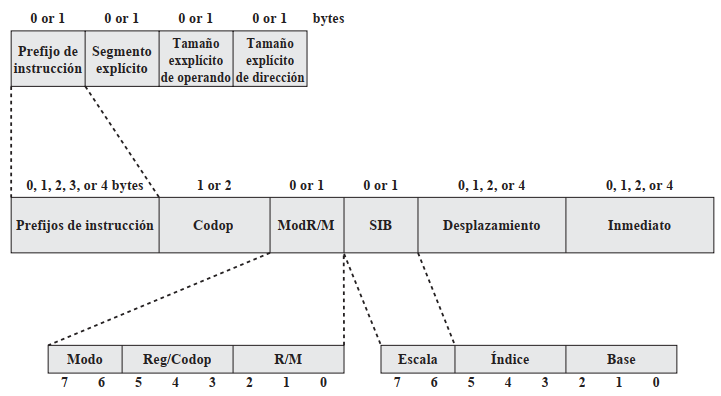
\includegraphics[width=1\linewidth]{images/formatoinstruccionx86} 

}

\caption{Formato de instrucciones del Pentium x86}\label{fig:FormatoInst}
\end{figure}

Un ejemplo típico de instrucción es:

\begin{lstlisting}
  ; Carga en el registro AX el valor almacenado en la dirección de memoria
  ; que resulta de sumar el contenido de los registros BX y SI más el desplazamiento 16.
  MOV AX, [BX+SI+16]
  \end{lstlisting}

Esta instrucción utiliza varios componentes, que el procesador debe decodificar antes de ejecutarla. Aunque esta flexibilidad es una ventaja en términos de funcionalidad, requiere técnicas avanzadas, como predicción de saltos y paralelización, para mantener la eficiencia en procesadores modernos \protect\hyperlink{ref-hennessy2017computer}{{[}19{]}}, \protect\hyperlink{ref-patterson_computer_2014}{{[}34{]}}, \protect\hyperlink{ref-brey_intel_microprocessors}{{[}50{]}}.

\hypertarget{lenguaje-muxe1quina-y-lenguaje-ensamblador}{%
\section{Lenguaje máquina y lenguaje ensamblador}\label{lenguaje-muxe1quina-y-lenguaje-ensamblador}}

El lenguaje máquina es el conjunto de instrucciones que un procesador puede entender y ejecutar directamente. Cada procesador tiene su propio conjunto de instrucciones, que se representan en forma de números binarios. Estas instrucciones son específicas para cada arquitectura y están diseñadas para realizar operaciones básicas como sumar, restar, mover datos entre registros y acceder a la memoria. El lenguaje máquina es el nivel más bajo de programación y está compuesto por secuencias de bits que representan operaciones y operandos específicos del procesador
\protect\hyperlink{ref-hennessy2017computer}{{[}19{]}}, \protect\hyperlink{ref-irvine2011assembly}{{[}52{]}}.

El procesador ejecuta directamente las instrucciones codificadas en lenguaje máquina, sin requerir traducción desde niveles superiores de abstracción. Sin embargo, la escritura manual de código en lenguaje máquina es un proceso extremadamente laborioso, propenso a errores y difícil de mantener. Cada instrucción debe representarse como una cadena precisa de ceros y unos. Esta codificación depende de las reglas específicas del procesador, que incluyen los modos de direccionamiento, los formatos de instrucción y la organización de la memoria \protect\hyperlink{ref-stallings_computer_2021}{{[}20{]}}, \protect\hyperlink{ref-tanenbaum_structured_2016}{{[}28{]}}, \protect\hyperlink{ref-null_essentials_2023}{{[}33{]}}, \protect\hyperlink{ref-irvine2011assembly}{{[}52{]}}.

Por ejemplo, si un estudiante o desarrollador deseara sumar dos números en lenguaje máquina, tendría que especificar manualmente cada secuencia binaria correspondiente a la operación de suma, así como las direcciones de memoria donde se encuentran los operandos. Este enfoque no solo es tedioso, sino que también aumenta la probabilidad de errores, especialmente cuando se requiere modificar o depurar el código.

Ante las limitaciones del lenguaje máquina en términos de legibilidad y mantenibilidad, se desarrolló un lenguaje de bajo nivel con mayor legibilidad que el lenguaje máquina que permitiera al programador escribir instrucciones de forma más comprensible: el lenguaje ensamblador. Este lenguaje permite a los programadores escribir instrucciones más comprensibles mediante mnemónicos simbólicos, que actúan como representaciones legibles de las instrucciones en lenguaje máquina. Cada arquitectura de procesador define su propio conjunto de instrucciones (ISA, Instruction Set Architecture), lo que implica que el lenguaje ensamblador asociado debe ajustarse a la codificación binaria, modos de direccionamiento y sintaxis específicos de dicha ISA \protect\hyperlink{ref-stallings_computer_2021}{{[}20{]}}.

En el ámbito educativo, el lenguaje ensamblador se destaca como una herramienta fundamental para comprender cómo se comunican el software y el hardware \protect\hyperlink{ref-tanenbaum_structured_2016}{{[}28{]}}, \protect\hyperlink{ref-null_essentials_2023}{{[}33{]}}. Permite a los estudiantes visualizar la ejecución de instrucciones individuales, analizar el uso de registros y explorar la estructura de la memoria, convirtiéndose en un recurso valioso para este propósito.

Un programa en lenguaje ensamblador suele estar compuesto por instrucciones que especifican un mnemónico, uno o más operandos, y eventualmente el modo de direccionamiento. Por ejemplo:

\begin{lstlisting}
  ; Carga el valor inmediato 5 en el registro AX.
  MOV AX, 5  

  ; Sumar los registros BX y AX, guarda el resultado en AX.
  ADD AX, BX 
  \end{lstlisting}

Estas líneas indican que el valor 5 se mueve al registro AX y luego se suma el contenido de BX. A través de este tipo de instrucciones, el estudiante puede visualizar de forma explícita cómo opera el procesador sobre sus registros y memoria.

\hypertarget{ensamblador}{%
\subsection{Ensamblador}\label{ensamblador}}

El ensamblador es un programa que traduce las instrucciones simbólicas escritas en lenguaje ensamblador a lenguaje máquina, es decir, las convierte en las secuencias binarias que el procesador puede interpretar y ejecutar. Este proceso de traducción es prácticamente directo, ya que existe una correspondencia uno a uno entre las instrucciones en ensamblador y las instrucciones en lenguaje máquina \protect\hyperlink{ref-stallings_computer_2021}{{[}20{]}}, \protect\hyperlink{ref-tanenbaum_structured_2016}{{[}28{]}}. En contraste, los lenguajes de programación de alto nivel, como C o Python, suelen generar múltiples instrucciones máquina por cada línea de código fuente, lo que los distancia más de la arquitectura subyacente \protect\hyperlink{ref-hennessy2017computer}{{[}19{]}}.

La Figura \ref{fig:ensambla} muestra el proceso de traducción de un programa en lenguaje ensamblador a lenguaje máquina. En este proceso, el ensamblador toma cada línea de código en ensamblador y la convierte en su representación binaria correspondiente, generando así un archivo ejecutable que puede ser cargado y ejecutado por el procesador.

\begin{figure}

{\centering 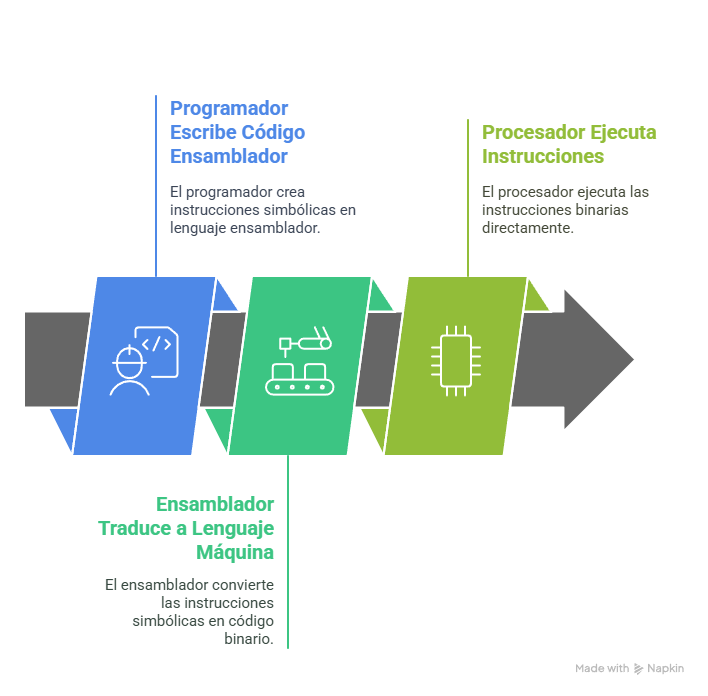
\includegraphics[width=1\linewidth]{images/ensamblador} 

}

\caption{Proceso de ensamblado}\label{fig:ensambla}
\end{figure}

\hypertarget{ensambladores-x86}{%
\subsection{Ensambladores x86}\label{ensambladores-x86}}

En el caso de la arquitectura x86, los programadores pueden elegir entre diversos ensambladores, como TASM (Turbo Assembler) \protect\hyperlink{ref-tasm}{{[}53{]}}, MASM (Microsoft Macro Assembler) \protect\hyperlink{ref-masm}{{[}54{]}} y NASM (Netwide Assembler) \protect\hyperlink{ref-nasm}{{[}55{]}}. Aunque cada ensamblador tiene características y sintaxis particulares, todos comparten el objetivo fundamental de convertir las instrucciones ensamblador en código binario ejecutable por los procesadores x86 \protect\hyperlink{ref-hyde2010art}{{[}56{]}}.

A continuación, se presenta una tabla comparativa \ref{tab:ensambladores} que resume las principales características de tres ensambladores ampliamente utilizados en la arquitectura x86. La información compilada permite visualizar diferencias relevantes en términos de sintaxis, compatibilidad, funcionalidades adicionales y contexto de uso, lo que resulta particularmente útil al momento de seleccionar herramientas adecuadas para entornos educativos o de desarrollo de bajo nivel.

\begin{table}[!h]
\centering
\caption{\label{tab:ensambladores}Comparación de ensambladores arquitectura x86}
\centering
\resizebox{\ifdim\width>\linewidth\linewidth\else\width\fi}{!}{
\fontsize{10}{12}\selectfont
\begin{tabular}[t]{>{\raggedright\arraybackslash}p{3cm}|>{\raggedright\arraybackslash}p{4cm}>{\raggedright\arraybackslash}p{4cm}>{\raggedright\arraybackslash}p{4cm}}
\toprule
\multicolumn{1}{>{\centering\arraybackslash}p{3cm}}{\cellcolor[HTML]{D3D3D3}{\textbf{Característica}}} & \multicolumn{1}{>{\centering\arraybackslash}p{4cm}}{\cellcolor[HTML]{D3D3D3}{\textbf{TASM}}} & \multicolumn{1}{>{\centering\arraybackslash}p{4cm}}{\cellcolor[HTML]{D3D3D3}{\textbf{MASM}}} & \multicolumn{1}{>{\centering\arraybackslash}p{4cm}}{\cellcolor[HTML]{D3D3D3}{\textbf{NASM}}}\\
\midrule
\textbf{Desarrollador} & Borland & Microsoft & Simon Tatham et al.\\
\addlinespace[10pt]
\textbf{Año de lanzamiento} & 1985 & 1981 & 1996\\
\addlinespace[10pt]
\textbf{Sistema operativo} & MS-DOS, Windows & MS-DOS, Windows & Multiplataforma (Windows, Linux, macOS)\\
\addlinespace[10pt]
\textbf{Sintaxis} & Sintaxis similar a Intel con extensiones & Sintaxis de Intel con soporte avanzado & Sintaxis de Intel, modular y extensible\\
\addlinespace[10pt]
\textbf{Soporte de macros} & Macros y directivas avanzadas & Macros y directivas extensivas & Macros avanzadas y preprocesamiento\\
\addlinespace[10pt]
\addlinespace
\textbf{Compatibilidad} & Compatibilidad con x86 antiguo & Compatibilidad con x86 antiguo & Compatibilidad con x86, x86-64 y otros\\
\addlinespace[10pt]
\textbf{Capacidades adicionales} & Integración con herramientas Borland & Integración con Visual Studio & Soporte para múltiples formatos (binario, ELF, etc.)\\
\addlinespace[10pt]
\textbf{Licencia} & Comercial & Comercial & Código abierto\\
\addlinespace[10pt]
\textbf{Uso actual} & Menos común, usado en entornos heredados & Ampliamente usado en desarrollo Windows & Popular en sistemas y software libre\\
\addlinespace[10pt]
\bottomrule
\end{tabular}}
\end{table}

\hypertarget{simulacion}{%
\chapter{Simulación}\label{simulacion}}

En este capítulo se analiza el papel de la simulación desde una perspectiva didáctica, destacando su relevancia como herramienta de apoyo en la enseñanza de Arquitectura de Computadoras. Se abordan los beneficios que ofrecen los simuladores en el proceso educativo y los desafíos que ayudan a superar en la formación de los estudiantes.

\hypertarget{introducciuxf3n-a-la-simulaciuxf3n}{%
\section{Introducción a la simulación}\label{introducciuxf3n-a-la-simulaciuxf3n}}

La simulación constituye una herramienta esencial en múltiples dominios, incluidos la medicina, la defensa, el entretenimiento y particularmente la educación, debido a su capacidad para representar procesos complejos y facilitar la toma de decisiones en entornos seguros y controlados. Su principal valor radica en su capacidad para modelar sistemas complejos, generar hipótesis, realizar análisis predictivos y explorar escenarios de manera segura y eficiente.

Banks define la simulación como el proceso de replicar el comportamiento de un sistema a lo largo del tiempo mediante un modelo conceptual que representa sus características y dinámicas principales \protect\hyperlink{ref-banks_discrete-event_2010}{{[}2{]}}. Estos modelos evolucionan simulando las interacciones entre sus componentes, lo que permite estudiar su respuesta ante diferentes variables y escenarios \protect\hyperlink{ref-robinson_simulation_2014}{{[}4{]}}.

La posibilidad de analizar sistemas complejos sin intervenir directamente en ellos convierte a la simulación en una herramienta indispensable en el contexto actual, marcado por el avance de la tecnología y la creciente complejidad de los sistemas. Además, la simulación permite optimizar diseños, prever comportamientos y reducir los costos de desarrollo antes de implementar soluciones reales \protect\hyperlink{ref-law_simulation_2015}{{[}3{]}}, \protect\hyperlink{ref-zeigler_theory_2000}{{[}26{]}}.

\hypertarget{aplicaciones-de-la-simulaciuxf3n-en-la-industria}{%
\subsection{Aplicaciones de la simulación en la industria}\label{aplicaciones-de-la-simulaciuxf3n-en-la-industria}}

En sectores como la industria automotriz, la simulación es fundamental para el diseño y prueba de sistemas de seguridad, como airbags y frenos. Gracias a modelos virtuales, se realizan pruebas de colisión y análisis de rendimiento sin necesidad de recurrir a costosas pruebas físicas. Asimismo, la simulación permite optimizar diseños de motores, analizar el flujo aerodinámico y prever el comportamiento de materiales en condiciones extremas, contribuyendo a mejorar tanto la eficiencia como la seguridad de los vehículos \protect\hyperlink{ref-stork_towards_2008}{{[}57{]}}.

En la aviación, los simuladores de vuelo son esenciales para entrenar pilotos, replicando condiciones reales de vuelo sin riesgos. Durante el diseño de aeronaves, estas herramientas permiten evaluar la aerodinámica y el rendimiento en diversos entornos, reduciendo significativamente el tiempo y los costos de desarrollo mientras incrementan la seguridad \protect\hyperlink{ref-jentsch_simulation_2017}{{[}58{]}}.

Estos principios generales encuentran aplicaciones concretas en diversos sectores industriales, donde la simulación cumple un papel clave tanto en el diseño como en el entrenamiento, la evaluación y la toma de decisiones.

\begin{table}[!h]
\centering
\caption{\label{tab:unnamed-chunk-2}Aplicaciones de la simulación en distintos sectores}
\centering
\resizebox{\ifdim\width>\linewidth\linewidth\else\width\fi}{!}{
\fontsize{10}{12}\selectfont
\begin{tabular}[t]{>{\raggedright\arraybackslash}p{3cm}|>{\raggedright\arraybackslash}p{6cm}>{\raggedright\arraybackslash}p{6cm}}
\toprule
\multicolumn{1}{>{\centering\arraybackslash}p{3cm}}{\cellcolor[HTML]{D3D3D3}{\textbf{Sector}}} & \multicolumn{1}{>{\centering\arraybackslash}p{6cm}}{\cellcolor[HTML]{D3D3D3}{\textbf{Aplicación}}} & \multicolumn{1}{>{\centering\arraybackslash}p{6cm}}{\cellcolor[HTML]{D3D3D3}{\textbf{Beneficio principal}}}\\
\midrule
\textbf{Automotriz} & Pruebas de colisión virtuales & Reducción de costos y aumento de seguridad\\
\addlinespace[10pt]
\textbf{Aeroespacial} & Simuladores de vuelo & Entrenamiento sin riesgo\\
\addlinespace[10pt]
\textbf{Medicina} & Simulación de cirugías & Entrenamiento sin comprometer pacientes\\
\addlinespace[10pt]
\textbf{Educación} & Simuladores para arquitectura de computadoras & Comprensión de procesos abstractos\\
\addlinespace[10pt]
\bottomrule
\end{tabular}}
\end{table}

Estos ejemplos ilustran cómo la simulación contribuye significativamente a la optimización de procesos, la reducción de riesgos y la mejora continua en el desarrollo de sistemas complejos. Su uso no solo ha transformado sectores productivos, sino que también ofrece un modelo replicable en contextos educativos especializados, como la enseñanza de arquitectura de computadoras.

\hypertarget{simulaciuxf3n-en-la-educaciuxf3n}{%
\section{Simulación en la educación}\label{simulaciuxf3n-en-la-educaciuxf3n}}

En contextos educativos, la simulación se ha consolidado como una estrategia pedagógica eficaz para facilitar la comprensión de fenómenos complejos, especialmente en disciplinas que requieren alto nivel de abstracción y razonamiento sistémico. A través de simuladores, los estudiantes pueden interactuar con sistemas virtuales y experimentar escenarios realistas, lo que mejora la comprensión de ideas abstractas y favorece la aplicación práctica de conocimientos teóricos \protect\hyperlink{ref-lion_simuladores_2005}{{[}5{]}}.

En contraste con enfoques instruccionales tradicionales centrados en la transmisión de información, los simuladores favorecen metodologías activas basadas en el aprendizaje por descubrimiento, la resolución de problemas y la construcción significativa del conocimiento, las herramientas de simulación integran tecnologías que vinculan conceptos teóricos con situaciones reales. Esto promueve una pedagogía interactiva, basada en la resolución de problemas y el aprendizaje por descubrimiento, estimulando la exploración y el razonamiento inferencial \protect\hyperlink{ref-contreras_uso_2010}{{[}6{]}}.

En definitiva, la simulación enriquece la experiencia de aprendizaje al proporcionar una plataforma dinámica y participativa que facilita tanto la experimentación como la asimilación profunda de los contenidos.

\hypertarget{el-rol-de-la-simulaciuxf3n-en-la-enseuxf1anza-de-arquitectura-de-computadoras}{%
\subsection{El rol de la simulación en la enseñanza de Arquitectura de Computadoras}\label{el-rol-de-la-simulaciuxf3n-en-la-enseuxf1anza-de-arquitectura-de-computadoras}}

En la carrera de Licenciatura en Sistemas, la asignatura Arquitectura de Computadoras persigue varios objetivos esenciales:
- Comprender la estructura y funcionamiento de las computadoras.
- Conocer las diferentes arquitecturas de sistemas microprocesadores.
- Evaluar medidas de rendimiento y comparar arquitecturas.
- Analizar el impacto de la tecnología de las computadoras en contextos sociales y económicos.

Enseñar los fundamentos teóricos de la organización y arquitectura interna de las computadoras puede ser un reto debido a la complejidad de los procesos involucrados. Los estudiantes necesitan desarrollar altos niveles de abstracción para construir modelos mentales que les permitan entender conceptos como la ejecución de instrucciones, la gestión de memoria o la interacción entre componentes del sistema.

En este contexto, los simuladores se configuran como mediadores didácticos que permiten representar gráficamente procesos abstractos, facilitando la manipulación de parámetros y el análisis de resultados en un entorno seguro, repetible y sin restricciones físicas. Estas herramientas permiten a los alumnos experimentar con configuraciones y parámetros, observar su impacto en el rendimiento del sistema y explorar escenarios hipotéticos sin necesidad de hardware físico.

Además, la simulación actúa como un puente entre la teoría y la práctica, facilitando que los docentes refuercen conceptos abstractos con experiencias concretas. En conjunto, estas ventajas hacen de la simulación una metodología pedagógica invaluable, promoviendo la experimentación y el aprendizaje activo en la enseñanza de Arquitectura de Computadoras \protect\hyperlink{ref-garcia-garcia_pbbcache_2020}{{[}7{]}}, \protect\hyperlink{ref-nova_tool_2013}{{[}12{]}}, \protect\hyperlink{ref-skrien_cpu_2001}{{[}24{]}}.

\hypertarget{el-formalismo-devs-discrete-event-system-specification}{%
\section{El Formalismo DEVS (Discrete Event System Specification)}\label{el-formalismo-devs-discrete-event-system-specification}}

El formalismo DEVS es una metodología modular y jerárquica que permite modelar y analizar sistemas representables como sistemas de eventos discretos, continuos o híbridos. Desarrollado por Bernard P. Zeigler en la década de 1970, este enfoque amplía el concepto de las máquinas de Moore al añadir una estructura que permite representar el comportamiento de sistemas mediante eventos temporizados que provocan cambios de estado, capturando así tanto la dinámica interna como las interacciones externas del sistema \protect\hyperlink{ref-zeigler_theory_2000}{{[}26{]}}.

\hypertarget{estructura-del-formalismo-devs}{%
\subsection{Estructura del formalismo DEVS}\label{estructura-del-formalismo-devs}}

El formalismo DEVS se basa en la representación de sistemas como una colección de componentes que interactúan entre sí a través de eventos. Cada componente tiene un estado interno y puede recibir eventos externos que provocan cambios en su estado. Estos eventos pueden ser temporizados, lo que significa que el sistema puede reaccionar a eventos en momentos específicos, o pueden ser desencadenados por condiciones específicas.
Esta estructura permite capturar tanto el comportamiento interno como la interacción externa del sistema modelado, ver figura \ref{fig:devs}.

\begin{figure}

{\centering 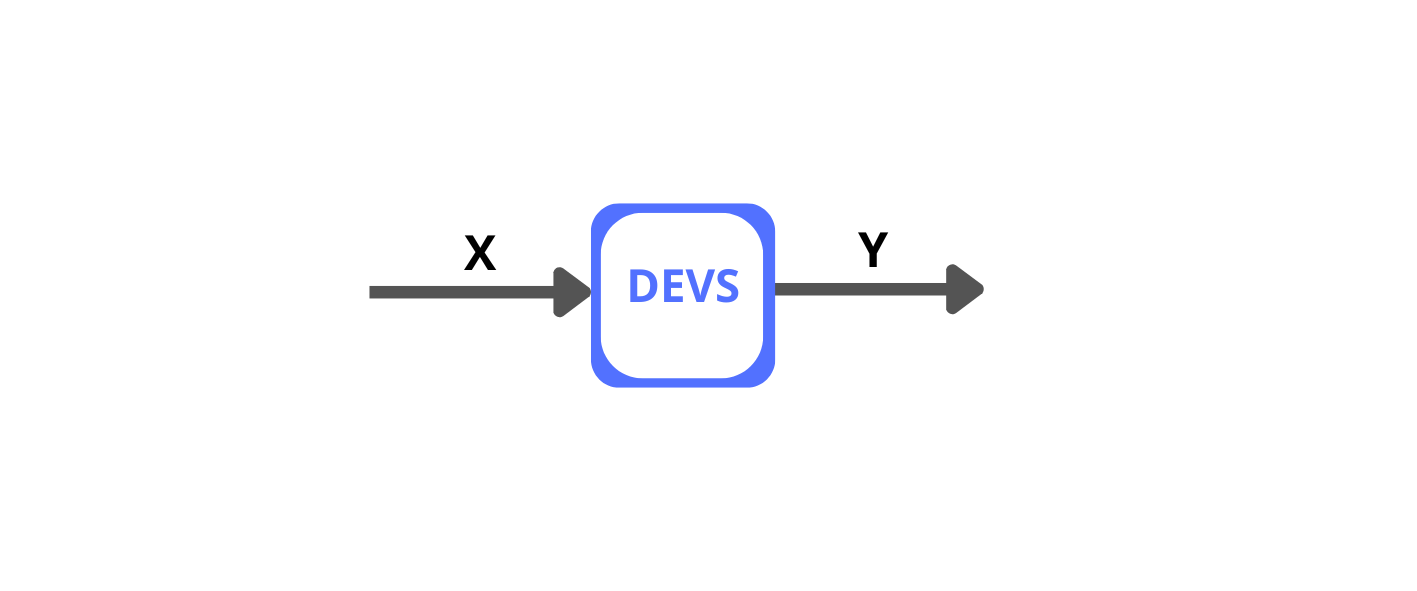
\includegraphics[width=1\linewidth]{images/devs} 

}

\caption{Relación entre modelos atómicos y modelos acoplados en DEVS}\label{fig:devs}
\end{figure}

DEVS describe el comportamiento de un sistema real utilizando eventos de entrada y salida, así como transiciones entre estados definidos. Un sistema en este formalismo se compone de dos tipos principales de modelos:

\begin{itemize}
\tightlist
\item
  \textbf{Modelos atómicos}: representan las unidades fundamentales de comportamiento.
\item
  \textbf{Modelos acoplados}: integran modelos atómicos y/o otros modelos acoplados, permitiendo la construcción jerárquica de sistemas más complejos.
\end{itemize}

Esta organización modular facilita el análisis y la gestión de sistemas, permitiendo probar subsistemas de manera aislada antes de integrarlos en un modelo completo.

La siguiente figura \ref{fig:acoplado} ilustra la organización modular del formalismo DEVS, mostrando cómo se integran modelos atómicos dentro de modelos acoplados:

\begin{figure}

{\centering 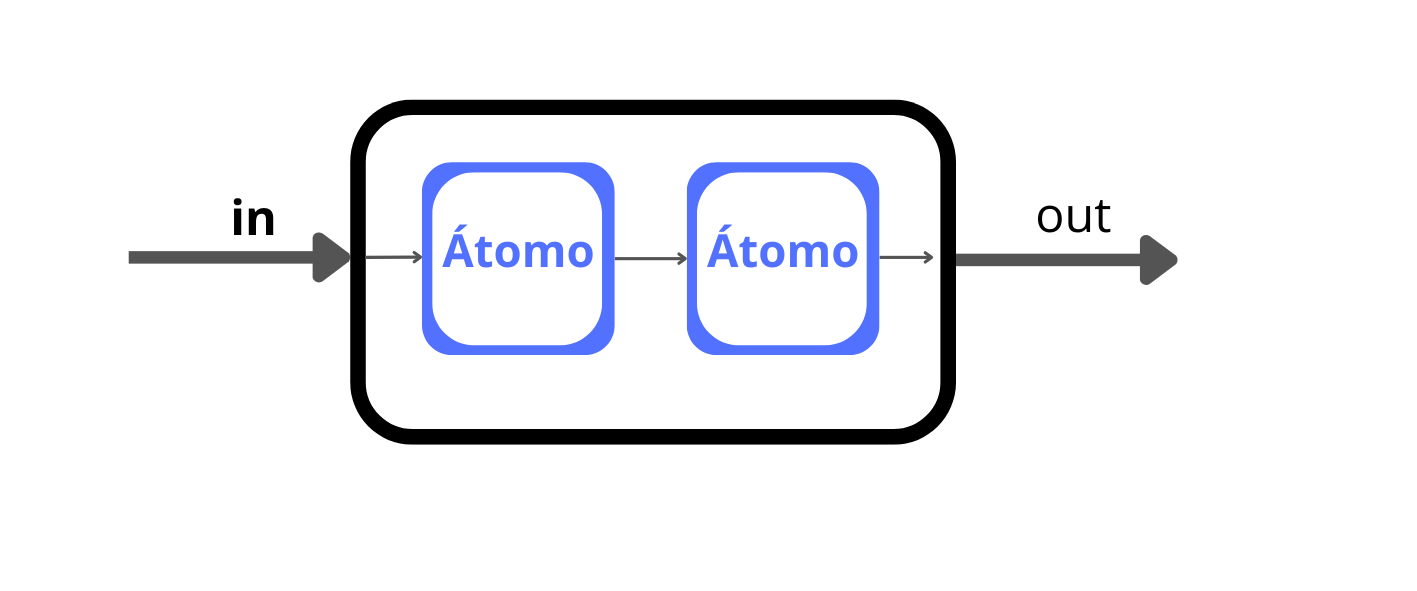
\includegraphics[width=1\linewidth]{images/acoplado} 

}

\caption{Modelo acoplado en DEVS}\label{fig:acoplado}
\end{figure}

\hypertarget{aplicaciones-del-formalismo-devs}{%
\subsection{Aplicaciones del formalismo DEVS}\label{aplicaciones-del-formalismo-devs}}

``El formalismo DEVS encuentra aplicación en diversos ámbitos, como las redes de comunicación \protect\hyperlink{ref-fujimoto2001parallel}{{[}59{]}}, donde permite simular el enrutamiento de paquetes y la congestión de redes; en entornos de manufactura \protect\hyperlink{ref-zeigler_theory_2000}{{[}26{]}}, donde se modelan flujos de producción y control de calidad; y en sistemas de transporte, para la optimización de flujos vehiculares \protect\hyperlink{ref-barros1997modeling}{{[}60{]}}. También se utiliza en la simulación de sistemas biológicos, como la propagación de enfermedades o el comportamiento de poblaciones \protect\hyperlink{ref-zeigler2004continuity}{{[}61{]}}. En el ámbito de la educación, DEVS se ha implementado en simuladores para la enseñanza de arquitectura de computadoras, permitiendo a los estudiantes explorar y comprender conceptos complejos mediante la visualización y manipulación de modelos \protect\hyperlink{ref-calvo2010simulador}{{[}62{]}}.

Estas aplicaciones destacan su versatilidad para optimizar sistemas complejos en escenarios del mundo real.

\hypertarget{devs-en-la-enseuxf1anza-de-la-arquitectura-de-computadoras}{%
\subsection{DEVS en la enseñanza de la Arquitectura de Computadoras}\label{devs-en-la-enseuxf1anza-de-la-arquitectura-de-computadoras}}

La implementación de entornos de simulación basados en DEVS en la enseñanza de arquitectura de computadoras aporta múltiples ventajas que enriquecen el proceso de aprendizaje:

\begin{itemize}
\tightlist
\item
  \textbf{Representación visual}: ofrece diagramas y representaciones dinámicas que ayudan a los estudiantes a visualizar y comprender procesos internos, como la ejecución de instrucciones y la gestión de recursos.
\item
  \textbf{Interactividad}: permite modificar configuraciones y parámetros, fomentando la experimentación y mostrando el impacto directo de estas variables en el rendimiento del sistema.
\item
  \textbf{Exploración de escenarios}: posibilita simular escenarios hipotéticos y evaluar el comportamiento de sistemas complejos sin la necesidad de hardware físico.
\end{itemize}

Estas funcionalidades enriquecen la experiencia educativa al integrar la teoría con la práctica y fomentar una participación activa en el análisis de los principios fundamentales de la arquitectura computacional. Al adoptar DEVS como parte del entorno educativo, se potencia la capacidad de los estudiantes para abordar problemas complejos y explorar soluciones innovadoras \protect\hyperlink{ref-calvo_valdes_simulador_2010}{{[}63{]}}.

En conclusión, el formalismo DEVS no solo es una herramienta valiosa para el modelado y análisis de sistemas, sino que también representa un recurso poderoso para facilitar la enseñanza de conceptos complejos, como los que se encuentran en la arquitectura de computadoras.

\hypertarget{comparativa}{%
\chapter{Comparativa de simuladores}\label{comparativa}}

Este capítulo presenta un análisis comparativo de simuladores basados en la arquitectura x86, con el objetivo de determinar su adecuación para su integración en la asignatura Arquitectura de Computadoras de la Licenciatura en Sistemas de Información.

La selección y evaluación de estos simuladores se fundamenta en criterios específicos diseñados para medir su efectividad en un entorno educativo. El objetivo principal es identificar las herramientas que mejor respalden el proceso de enseñanza y aprendizaje. Los criterios definidos abarcan aspectos clave para la enseñanza de arquitectura de computadoras: facilidad de uso, funcionalidades del entorno de programación, calidad de los recursos de apoyo, mecanismos de ejecución de programas, precisión en la emulación de la arquitectura x86, características técnicas del software y su alineación con los contenidos curriculares.

Los resultados de esta investigación fueron publicados en el XVII Congreso de Tecnología en Educación y Educación en Tecnología (2022), en el trabajo titulado Herramientas de software para dar soporte en la enseñanza y aprendizaje de la arquitectura x86 \protect\hyperlink{ref-colombani_herramientas_2022}{{[}64{]}}.

\hypertarget{estudios-similares}{%
\section{Estudios similares}\label{estudios-similares}}

Existen antecedentes de estudios comparativos que evalúan simuladores aplicados a la enseñanza en cursos de arquitectura de computadoras:
- ``A survey and evaluation of simulators suitable for teaching courses in computer architecture and organization'', 2009 \protect\hyperlink{ref-nikolic_survey_2009}{{[}17{]}}: este estudio analiza simuladores considerando dos categorías principales. La primera, relacionada con las características de simulación, incluye criterios como granularidad, usabilidad, disponibilidad, presentación visual y flujo de simulación. La segunda categoría evalúa la cobertura de los contenidos establecidos en los planes de estudio.
- ``Survey and evaluation of simulators suitable for teaching for computer architecture and organization Supporting undergraduate students at Sir Syed University of Engineering \& Technology'', 2012 \protect\hyperlink{ref-hasan_survey_2012}{{[}18{]}}: este trabajo evalúa aspectos como la usabilidad, disponibilidad, fundamentos de arquitectura informática, jerarquía de sistemas de memoria, comunicación e interfaz, y diseño de sistemas de procesadores.

A diferencia de los estudios mencionados, este trabajo propone una evaluación centrada exclusivamente en simuladores de arquitectura x86, mediante el uso de criterios diseñados ad hoc para analizar tanto las funcionalidades de simulación como su adecuación a los contenidos específicos de la asignatura Arquitectura de Computadoras dictada en la Licenciatura en Sistemas de la Universidad Nacional de Entre Ríos.

\hypertarget{simuladores-bajo-anuxe1lisis}{%
\section{Simuladores bajo análisis}\label{simuladores-bajo-anuxe1lisis}}

Un simulador de arquitectura es una herramienta de software que emula el hardware de un sistema de cómputo, permitiendo representar aspectos arquitectónicos y funcionales del mismo. Estos simuladores ofrecen un entorno controlado para realizar pruebas, modificaciones y ejecución de programas sin riesgo de dañar componentes físicos o enfrentar limitaciones de hardware \protect\hyperlink{ref-radivojevic_design_2011}{{[}16{]}}.

Algunos simuladores destacan por proporcionar una representación visual e interactiva de la organización y arquitectura interna de una computadora, facilitando la comprensión de su funcionamiento. Algunos ejemplos relevantes de simuladores son: Assembly Debugger (x86), Simple 8-bit Assembler Simulator, Microprocessor Simulator, Simulador de ensamblador de 16 bits y Emu8086. Estas herramientas juegan un papel fundamental en el aprendizaje de la arquitectura de computadoras, al conectar conceptos teóricos con experiencias prácticas y simplificar abstracciones complejas, además de servir como soporte en la labor docente \protect\hyperlink{ref-nikolic_survey_2009}{{[}17{]}}, \protect\hyperlink{ref-hasan_survey_2012}{{[}18{]}}, \protect\hyperlink{ref-hennessy2017computer}{{[}19{]}}, \protect\hyperlink{ref-stallings_computer_2021}{{[}20{]}}, \protect\hyperlink{ref-behrooz_computer_2005}{{[}65{]}}.

\hypertarget{criterios-de-evaluaciuxf3n}{%
\section{Criterios de evaluación}\label{criterios-de-evaluaciuxf3n}}

Los criterios de evaluación se definieron con el objetivo de realizar un análisis integral y sistemático de los simuladores seleccionados. A continuación, se presentan estos criterios junto con sus respectivos indicadores y escalas:

\begin{itemize}
\tightlist
\item
  \textbf{Usabilidad}: evalúa la facilidad de uso del simulador.

  \begin{itemize}
  \tightlist
  \item
    \textbf{Indicadores}:

    \begin{itemize}
    \tightlist
    \item
      Facilidad de aprendizaje (tiempo necesario para familiarizarse con la herramienta).
    \item
      Interfaz de usuario (claridad y organización).
    \item
      Documentación y ayuda (accesibilidad y calidad de tutoriales y guías).
    \end{itemize}
  \item
    \textbf{Escala}: Difícil - Media - Fácil.
  \end{itemize}
\item
  \textbf{Editor}: analiza las funcionalidades para escribir y depurar código ensamblador.

  \begin{itemize}
  \tightlist
  \item
    \textbf{Indicadores}:

    \begin{itemize}
    \tightlist
    \item
      Capacidad de edición (resaltado de sintaxis, puntos de interrupción, etc.).
    \item
      Manejo de errores de sintaxis.
    \item
      Opciones de almacenamiento (guardar y cargar programas).
    \end{itemize}
  \item
    \textbf{Escala}: Baja - Media - Alta.
  \end{itemize}
\item
  \textbf{Documentación}: valora la disponibilidad y calidad de los recursos de aprendizaje proporcionados.

  \begin{itemize}
  \tightlist
  \item
    \textbf{Indicadores}:

    \begin{itemize}
    \tightlist
    \item
      Manual de usuario.
    \item
      Tutoriales de aprendizaje.
    \item
      Exhaustividad en la descripción del repertorio de instrucciones.
    \end{itemize}
  \item
    \textbf{Escala}: Mínima - Media - Completa.
  \end{itemize}
\item
  \textbf{Ejecución de simulación}: mide la facilidad para controlar y observar la ejecución de programas.

  \begin{itemize}
  \tightlist
  \item
    \textbf{Indicadores}:

    \begin{itemize}
    \tightlist
    \item
      Control de simulación (pausa, reanudación, retroceso).
    \item
      Visualización del flujo de ejecución.
    \item
      Configurabilidad (ajuste de parámetros como la velocidad del reloj).
    \end{itemize}
  \item
    \textbf{Escala}: Baja - Media - Alta.
  \end{itemize}
\item
  \textbf{Nivel de especificación de la Organización y Arquitectura del sistema simulado}: determina la precisión en la representación de la arquitectura x86.

  \begin{itemize}
  \tightlist
  \item
    \textbf{Indicadores}:

    \begin{itemize}
    \tightlist
    \item
      Fidelidad en la representación de la arquitectura.
    \item
      Completitud del conjunto de instrucciones implementadas.
    \item
      Inclusión y funcionalidad de memoria y módulos de E/S.
    \end{itemize}
  \item
    \textbf{Escala}: Mínima - Media - Completa.
  \end{itemize}
\item
  \textbf{Características del producto software}: evalúa las propiedades generales del simulador.

  \begin{itemize}
  \tightlist
  \item
    \textbf{Indicadores}:

    \begin{itemize}
    \tightlist
    \item
      Tipo de licencia (open source o privativa).
    \item
      Frecuencia de actualizaciones.
    \item
      Plataforma (aplicación web o de escritorio)
    \end{itemize}
  \item
    \textbf{Escala}: Mala - Buena - Muy buena.
  \end{itemize}
\item
  \textbf{Cobertura de los contenidos preestablecidos en la currícula}: mide el grado en que el simulador abarca los contenidos de la asignatura.

  \begin{itemize}
  \tightlist
  \item
    \textbf{Indicadores}:

    \begin{itemize}
    \tightlist
    \item
      Alineación con los tópicos del currículum.
    \item
      Profundidad en el tratamiento de los temas.
    \end{itemize}
  \item
    \textbf{Escala}: Baja - Media - Alta.
  \end{itemize}
\end{itemize}

La Tabla \ref{tab:criterios} resume los criterios, indicadores y escalas utilizadas.

\begin{table}[!h]
\centering
\caption{\label{tab:criterios}Criterios e indicadores de evaluación de simuladores}
\centering
\resizebox{\ifdim\width>\linewidth\linewidth\else\width\fi}{!}{
\fontsize{10}{12}\selectfont
\begin{tabular}[t]{>{\centering\arraybackslash}p{4cm}|>{\raggedright\arraybackslash}p{6cm}>{\raggedright\arraybackslash}p{6cm}}
\toprule
\multicolumn{1}{>{\centering\arraybackslash}p{4cm}}{\cellcolor[HTML]{D3D3D3}{\textbf{Criterio}}} & \multicolumn{1}{>{\centering\arraybackslash}p{6cm}}{\cellcolor[HTML]{D3D3D3}{\textbf{Indicadores}}} & \multicolumn{1}{>{\centering\arraybackslash}p{6cm}}{\cellcolor[HTML]{D3D3D3}{\textbf{Escala}}}\\
\midrule
\textbf{Usabilidad} & Facilidad de aprendizaje, interfaz, documentación & Difícil - Media - Fácil\\
\addlinespace[10pt]
\textbf{Funcionalidad del editor} & Sintaxis, manejo de errores, guardar/cargar & Baja - Media - Alta\\
\addlinespace[10pt]
\textbf{Calidad de la documentación} & Manuales, tutoriales, repertorio de instrucciones & Mínima - Media - Completa\\
\addlinespace[10pt]
\textbf{Ejecución de simulación} & Control de simulación, visualización del flujo, configurabilidad & Baja - Media - Alta\\
\addlinespace[10pt]
\textbf{Especificación de arquitectura x86} & Fidelidad de la arquitectura, repertorio, memoria y E/S & Mínima - Media - Completa\\
\addlinespace[10pt]
\addlinespace
\textbf{Propiedades técnicas y de distribución} & Licencia, actualizaciones, plataforma & Mala - Buena - Muy buena\\
\addlinespace[10pt]
\textbf{Alineación con contenidos curriculares} & Cobertura de tópicos, profundidad del tratamiento & Baja - Media - Alta\\
\addlinespace[10pt]
\bottomrule
\end{tabular}}
\end{table}

\hypertarget{selecciuxf3n-de-simuladores}{%
\section{Selección de simuladores}\label{selecciuxf3n-de-simuladores}}

Mediante una exploración exhaustiva de fuentes disponibles en línea, foros académicos y repositorios educativos, se identificaron los siguientes simuladores de arquitectura x86: Assembly Debugger (x86), Simple 8-bit Assembler Simulator, Microprocessor Simulator, Simulador de ensamblador de 16 bits, Emu8086, VonSim, Orga1 y Qsim. Estos simuladores fueron seleccionados por su relevancia en el ámbito educativo y su potencial para facilitar la enseñanza de la arquitectura x86.

La selección se basó en una evaluación preliminar que consideró el tiempo necesario para su análisis y el grado de cumplimiento de los criterios definidos, priorizando aquellos simuladores que ofrecieran un balance adecuado entre funcionalidad, usabilidad, documentación y alineación con los contenidos curriculares de la asignatura Arquitectura de Computadoras. De esta preselección, se eligieron tres herramientas que, a priori, cumplían con la mayor cantidad de criterios evaluativos: \textbf{Emu8086}, \textbf{VonSim} y \textbf{Simple 8-bit Assembler Simulator}.

\begin{table}[!h]
\centering
\caption{\label{tab:simuladores}Proceso de selección de simuladores}
\centering
\resizebox{\ifdim\width>\linewidth\linewidth\else\width\fi}{!}{
\fontsize{10}{12}\selectfont
\begin{tabular}[t]{>{\centering\arraybackslash}p{6cm}|>{\centering\arraybackslash}p{4cm}>{\centering\arraybackslash}p{4cm}}
\toprule
\multicolumn{1}{>{\centering\arraybackslash}p{6cm}}{\cellcolor[HTML]{D3D3D3}{\textbf{Simulador}}} & \multicolumn{1}{>{\centering\arraybackslash}p{4cm}}{\cellcolor[HTML]{D3D3D3}{\textbf{Exploración Previa}}} & \multicolumn{1}{>{\centering\arraybackslash}p{4cm}}{\cellcolor[HTML]{D3D3D3}{\textbf{Evaluación Final}}}\\
\midrule
\textbf{Assembly Debugger (x86)} & \checkmark & \ding{55}\\
\addlinespace[10pt]
\textbf{Simple 8-bit Assembler Simulator} & \checkmark & \checkmark\\
\addlinespace[10pt]
\textbf{Microprocessor Simulator} & \checkmark & \ding{55}\\
\addlinespace[10pt]
\textbf{Simulador de ensamblador de 16 bits} & \checkmark & \ding{55}\\
\addlinespace[10pt]
\textbf{Emu8086} & \checkmark & \checkmark\\
\addlinespace[10pt]
\addlinespace
\textbf{VonSim} & \checkmark & \checkmark\\
\addlinespace[10pt]
\textbf{Orga1} & \checkmark & \ding{55}\\
\addlinespace[10pt]
\textbf{Qsim} & \checkmark & \ding{55}\\
\addlinespace[10pt]
\bottomrule
\end{tabular}}
\end{table}

\hypertarget{participantes-en-la-evaluaciuxf3n}{%
\section{Participantes en la evaluación}\label{participantes-en-la-evaluaciuxf3n}}

La evaluación fue llevada a cabo por un equipo conformado por tres docentes de la asignatura Arquitectura de Computadoras ---Marcelo A. Colombani, José M. Ruiz y Amalia G. Delduca---, quienes aportaron su experiencia en el uso pedagógico de simuladores. Asimismo, se contó con la participación de un asesor externo, Marcelo A. Falappa, quien aportó una perspectiva independiente y validó tanto la metodología como los resultados obtenidos.

\hypertarget{anuxe1lisis-comparativo}{%
\section{Análisis comparativo}\label{anuxe1lisis-comparativo}}

A continuación, se presenta un análisis detallado de los simuladores seleccionados, basado en los criterios previamente establecidos:

\hypertarget{simple-8-bit-assembler-simulator}{%
\subsection{Simple 8-bit Assembler Simulator}\label{simple-8-bit-assembler-simulator}}

\begin{itemize}
\tightlist
\item
  \textbf{Usabilidad}: Nivel medio. Todos los componentes se muestran en una sola pantalla, lo que puede resultar abrumador para usuarios principiantes.
\item
  \textbf{Editor}: Nivel bajo. Incluye notificaciones de errores de sintaxis al ensamblar, pero carece de resaltado de sintaxis, puntos de interrupción (breakpoints) y opciones para guardar o cargar programas.
\item
  \textbf{Documentación}: Nivel mínimo. Consta solo de un manual de instrucciones implementadas.
\item
  \textbf{Ejecución de simulación}: Nivel medio. Permite ajustar la velocidad del reloj de la CPU y proporciona controles básicos de simulación.
\item
  \textbf{Nivel de especificación}: Nivel mínimo. Simplifica la arquitectura x86 a un CPU de 8 bits con 256 bytes de memoria y sin soporte para operaciones de entrada/salida (IN/OUT).
\item
  \textbf{Desarrollo del producto}: Nivel bueno. Licencia MIT, última actualización en 2015, desarrollado como una plataforma web.
\item
  \textbf{Cobertura de contenidos}: Nivel bajo. No incluye memoria independiente para módulos de entrada y salida, rutinas de interrupciones ni representación visual del ciclo de instrucción.
\end{itemize}

\hypertarget{vonsim}{%
\subsection{VonSim}\label{vonsim}}

\begin{itemize}
\tightlist
\item
  \textbf{Usabilidad}: Nivel medio. Utiliza solapas para presentar los componentes, lo que puede ser confuso para usuarios iniciales.
\item
  \textbf{Editor}: Nivel medio. Proporciona notificaciones de errores de sintaxis, resaltado de código y puntos de interrupción mediante software.
\item
  \textbf{Documentación}: Nivel medio. Incluye un manual de uso y un tutorial interactivo.
\item
  \textbf{Ejecución de simulación}: Nivel medio. Permite ajustar la velocidad del reloj de la CPU y ofrece controles básicos de simulación.
\item
  \textbf{Nivel de especificación}: Nivel medio. Representa una simplificación del procesador 8088 con arquitectura de 16 bits y memoria direccionable de 16 KiB.
\item
  \textbf{Desarrollo del producto}: Nivel muy bueno. Licencia GNU Affero General Public License v3.0, última versión en 2020, con amplia evidencia de uso académico.
\item
  \textbf{Cobertura de contenidos}: Nivel medio. Implementa dispositivos internos y externos, pero carece de visualización del ciclo de instrucción y métricas de rendimiento.
\end{itemize}

\hypertarget{emu8086}{%
\subsection{Emu8086}\label{emu8086}}

\begin{itemize}
\tightlist
\item
  \textbf{Usabilidad}: Nivel fácil. Inicialmente muestra el editor y permite activar los componentes del simulador a medida que se cargan programas.
\item
  \textbf{Editor}: Nivel alto. Incluye notificaciones de errores de sintaxis, resaltado de código, puntos de interrupción y opciones para guardar/cargar programas.
\item
  \textbf{Documentación}: Nivel completo. Ofrece un manual de instrucciones con ejemplos, un tutorial de aprendizaje y una guía de uso detallada.
\item
  \textbf{Ejecución de simulación}: Nivel alto. Proporciona control avanzado de la simulación, como retroceder una instrucción (``step back'').
\item
  \textbf{Nivel de especificación}: Nivel completo. Detalla la arquitectura del procesador 8086, con memoria direccionable de 1 MiB y soporte para interrupciones de software y hardware.
\item
  \textbf{Desarrollo del producto}: Nivel bueno. Licencia privativa, última actualización en 2023, desarrollado para plataformas de escritorio.
\item
  \textbf{Cobertura de contenidos}: Nivel alto. Emula el arranque (bootstrapping) de una IBM PC desde un disco flexible (floppy disk) y soporta todos los modos de direccionamiento.
\end{itemize}

\begin{table}[!h]
\centering
\caption{\label{tab:tabla-comparativa-criterios}Comparativa según criterios de evaluación preestablecidos}
\centering
\resizebox{\ifdim\width>\linewidth\linewidth\else\width\fi}{!}{
\fontsize{10}{12}\selectfont
\begin{tabular}[t]{>{\centering\arraybackslash}p{4cm}|>{\centering\arraybackslash}p{4cm}>{\centering\arraybackslash}p{4cm}>{\centering\arraybackslash}p{4cm}}
\toprule
\multicolumn{1}{>{\centering\arraybackslash}p{4cm}}{\cellcolor[HTML]{D3D3D3}{\textbf{Criterio de Evaluación}}} & \multicolumn{1}{>{\centering\arraybackslash}p{4cm}}{\cellcolor[HTML]{D3D3D3}{\textbf{Simple 8 bit}}} & \multicolumn{1}{>{\centering\arraybackslash}p{4cm}}{\cellcolor[HTML]{D3D3D3}{\textbf{VonSim}}} & \multicolumn{1}{>{\centering\arraybackslash}p{4cm}}{\cellcolor[HTML]{D3D3D3}{\textbf{Emu8086}}}\\
\midrule
\textbf{Usabilidad} & Medio & Medio & Fácil\\
\addlinespace[10pt]
\textbf{Editor} & Bajo & Medio & Alto\\
\addlinespace[10pt]
\textbf{Documentación} & Mínima & Media & Completa\\
\addlinespace[10pt]
\textbf{Ejecución de simulación} & Medio & Medio & Alta\\
\addlinespace[10pt]
\textbf{Nivel de especificación x86} & Mínima & Media & Completa\\
\addlinespace[10pt]
\addlinespace
\textbf{Características del producto} & Buena & Muy buena & Buena\\
\addlinespace[10pt]
\textbf{Cobertura de contenidos} & Baja & Media & Alta\\
\addlinespace[10pt]
\bottomrule
\end{tabular}}
\end{table}

\hypertarget{resultados}{%
\section{Resultados}\label{resultados}}

La asignatura promueve el uso de simuladores para apoyar la enseñanza y el aprendizaje, permitiendo aplicar los contenidos desarrollados en máquinas reales. Emu8086 es la herramienta más adecuada para esta finalidad, ya que facilita la implementación de programas en hardware real. Sin embargo, su dependencia de MS-DOS complica su ejecución en sistemas operativos actuales, requiriendo el uso de emuladores de MS-DOS, lo que añade complejidad al proceso de enseñanza y aprendizaje.

Desde 2018, la asignatura utiliza la versión 4.08 de Emu8086. La herramienta tiene un periodo de evaluación gratuito de 14 días, después del cual se debe adquirir una licencia. Esto es un inconveniente, ya que se busca que los estudiantes puedan acceder a las herramientas de forma libre y gratuita.

Utilizar lenguaje NASM (Netwide Assembler) garantiza soporte tanto para Linux como Windows a través de herramientas libres como GCC (GNU Compiler Collection), generando programas para la arquitectura x86 de 16, 32 y 64 bits.

Emu8086 destaca por su interfaz dinámica, que muestra componentes como la pila, flags, teclado y pantalla solo cuando son necesarios, a diferencia de otros simuladores que presentan todos sus componentes desde el inicio.

Emu8086 sobresale particularmente en los aspectos vinculados a la edición, documentación y control de la ejecución. Su editor permite establecer puntos de ruptura, retroceder una instrucción, y guardar o recuperar programas desde la interfaz. Además, ofrece una documentación extensa, que incluye un repertorio de instrucciones con ejemplos, un tutorial para el aprendizaje del lenguaje ensamblador y un manual detallado del entorno de desarrollo. Estas características lo posicionan como una herramienta completa en términos de acompañamiento a los procesos de enseñanza y aprendizaje.

En el criterio de evaluación cuatro, Emu8086 se destaca por ofrecer una mayor cantidad de controladores para gestionar el flujo de ejecución, como la capacidad de retroceder la ejecución de una instrucción y recargar el programa actual.

En cuanto al nivel de especificación, Emu8086 representa con gran precisión la arquitectura x86, incluyendo soporte para interrupciones del sistema operativo MS-DOS. Esta característica permite simular de manera realista programas que podrían ejecutarse en un entorno compatible, constituyendo una ventaja significativa frente a los otros simuladores analizados.

En el criterio de evaluación seis VonSim se destaca del resto debido a que es licencia libre y posee una comunidad que respalda el proyecto.

En cuanto al último criterio, ninguna de las herramientas evaluadas cubre todos los contenidos que se pretende desarrollar con la ayuda de una herramienta, quedando excluido pasos del ciclo de instrucción y medidas de rendimientos (tiempo de CPU y CPI: ciclo por instrucción).

A partir del análisis comparativo, se destacan las siguientes observaciones clave:

\begin{itemize}
\tightlist
\item
  \textbf{Emu8086} presenta la interfaz más intuitiva y completa, con amplia documentación y una simulación precisa de la arquitectura x86. Sin embargo, su licencia privativa y la necesidad de emuladores para su ejecución en sistemas actuales constituyen limitaciones relevantes.
\item
  \textbf{VonSim}, con su licencia libre y actualización reciente, representa una alternativa interesante desde una perspectiva de software abierto, aunque su cobertura de contenidos y nivel de especificación son limitados en comparación.
\item
  \textbf{Simple 8-bit Assembler Simulator} resulta insuficiente para cubrir los objetivos curriculares de la asignatura, debido a su bajo nivel de complejidad, escasa documentación y capacidades limitadas de simulación.
\end{itemize}

En conclusión, si bien cada simulador ofrece ventajas puntuales, ninguno logra satisfacer plenamente los requerimientos pedagógicos y técnicos de la asignatura en su totalidad. Por ello, se recomienda continuar utilizando Emu8086 de manera transitoria, mientras se avanza en el desarrollo de un simulador propio que integre sus fortalezas, opere con licencia libre y sea compatible con entornos modernos. Esta iniciativa permitirá una mayor adecuación curricular, accesibilidad tecnológica y sostenibilidad en el tiempo.

\hypertarget{publicaciuxf3n}{%
\subsection{Publicación}\label{publicaciuxf3n}}

Este análisis comparativo fue publicado en el XVII Congreso de Tecnología en Educación y Educación en Tecnología (2022), bajo el título ``Herramientas de software para dar soporte en la enseñanza y aprendizaje de la arquitectura x86''\protect\hyperlink{ref-colombani_herramientas_2022}{{[}64{]}}.

Además, durante este proceso se estableció contacto con un desarrollador de VonSim, logrando implementar mejoras significativas, como animaciones de ejecución y documentación en línea, disponibles en su última versión publicada en agosto de 2023.

\hypertarget{desarrollo}{%
\chapter{Diseño y construcción del simulador}\label{desarrollo}}

En este capítulo se describe el diseño y desarrollo de una herramienta de simulación específica para la arquitectura x86, orientada a facilitar la enseñanza de los principios de arquitectura de computadoras. Se detalla la justificación del diseño, los pasos seguidos para su construcción y los métodos utilizados para validar su funcionalidad.

En el capítulo anterior se analizaron y evaluaron las herramientas de simulación existentes para la arquitectura x86. Esta revisión exhaustiva permitió identificar las limitaciones de las soluciones actuales y fundamentar la necesidad de desarrollar una herramienta específica (véase el capítulo \ref{comparativa}).

A partir de esta necesidad, se establecieron un conjunto de requisitos funcionales y pedagógicos que guiaron de manera integral el diseño, la implementación y la validación del simulador. Estos requisitos no solo responden a las limitaciones observadas en herramientas existentes, sino que se alinean con los objetivos educativos previamente definidos.

\hypertarget{requisitos-de-la-herramienta}{%
\section{Requisitos de la herramienta}\label{requisitos-de-la-herramienta}}

Esta sección expone los requisitos que orientaron el diseño del simulador, clasificados en dos dimensiones complementarias: pedagógica y funcional. La primera se vincula con los objetivos formativos definidos en el capítulo introductorio (\ref{intro}), mientras que la segunda refiere a las características técnicas necesarias para garantizar su implementación eficaz. La definición de los requisitos se apoyó en principios pedagógicos y técnicos, complementados con una validación empírica realizada mediante entrevistas semiestructuradas a docentes expertos (ver Anexo A \ref{anexoA}). Este proceso permitió identificar necesidades auténticas del aula y carencias específicas en las herramientas existentes, aportando una base empírica rigurosa para la formulación pedagógica y técnica de los requisitos \protect\hyperlink{ref-huberman2019qualitative}{{[}66{]}}.

\begin{enumerate}
\def\labelenumi{\arabic{enumi}.}
\tightlist
\item
  \textbf{Visualización de la estructura general de la computadora:}
  Representar gráficamente la CPU, los buses, la memoria y los dispositivos de entrada/salida. Esta visualización debe destacar los componentes activos en cada etapa del ciclo de ejecución, facilitando una comprensión sistémica e integrada del funcionamiento de la computadora \protect\hyperlink{ref-w3c_accessibility_2021}{{[}67{]}}. El uso de representaciones gráficas como recurso didáctico está respaldado por estudios que demuestran su efectividad para facilitar la comprensión de conceptos abstractos en disciplinas técnicas \protect\hyperlink{ref-sorva2013visualizations}{{[}68{]}}. La Figura \ref{fig:diagramasimulador} ilustra la estructura general del simulador, destacando los principales módulos funcionales y sus interacciones. Esta representación gráfica facilita la comprensión de cómo los componentes del simulador trabajan en conjunto durante la ejecución de un programa.
\end{enumerate}

\begin{figure}

{\centering 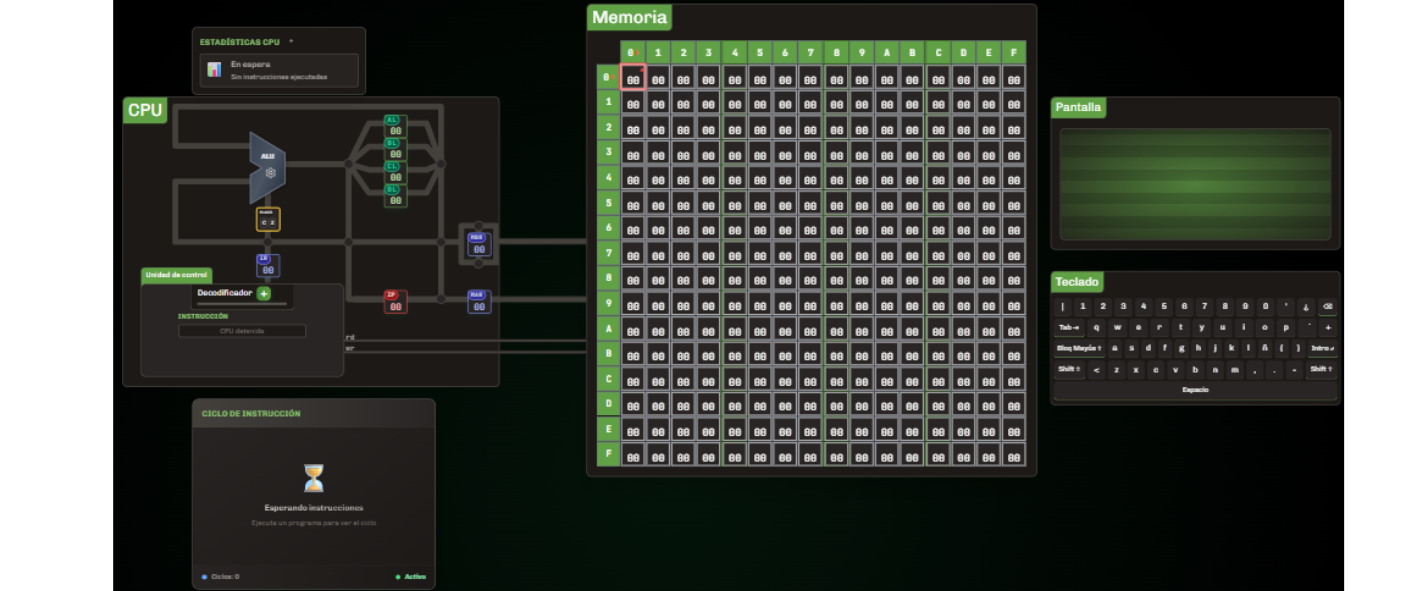
\includegraphics[width=0.9\linewidth]{images/estructurasimulador} 

}

\caption{Estructura del simulador y componentes funcionales}\label{fig:diagramasimulador}
\end{figure}

\begin{enumerate}
\def\labelenumi{\arabic{enumi}.}
\setcounter{enumi}{1}
\tightlist
\item
  \textbf{Soporte para la generación y ejecución de programas en ensamblador:}
  Incorporar la posibilidad de ejecutar programas escritos en lenguaje ensamblador tanto de forma paso a paso como en ejecución continua. Esta funcionalidad posibilita el análisis detallado de cada instrucción, fortaleciendo competencias en trazado y depuración de código ensamblador, fundamentales para comprender la relación entre software y hardware.
  Para apoyar este proceso, se propone la inclusión de un editor de ensamblador que incorpore funciones como resaltado de sintaxis y autocompletado. Estas características mejoran la experiencia del usuario y facilitan la escritura y comprensión del código, en consonancia con principios de diseño de interfaces que priorizan la usabilidad y la accesibilidad \protect\hyperlink{ref-w3c_accessibility_2021}{{[}67{]}}. El editor debe permitir al usuario escribir, editar, guardar y ejecutar programas en ensamblador dentro del simulador, además de ofrecer ejemplos predefinidos como apoyo didáctico. La incorporación de entornos de desarrollo integrados (IDEs) en contextos educativos ha demostrado ser eficaz para la enseñanza de lenguajes de programación, según diversos estudios \protect\hyperlink{ref-mccracken2001does}{{[}69{]}}.
\end{enumerate}

\begin{figure}

{\centering 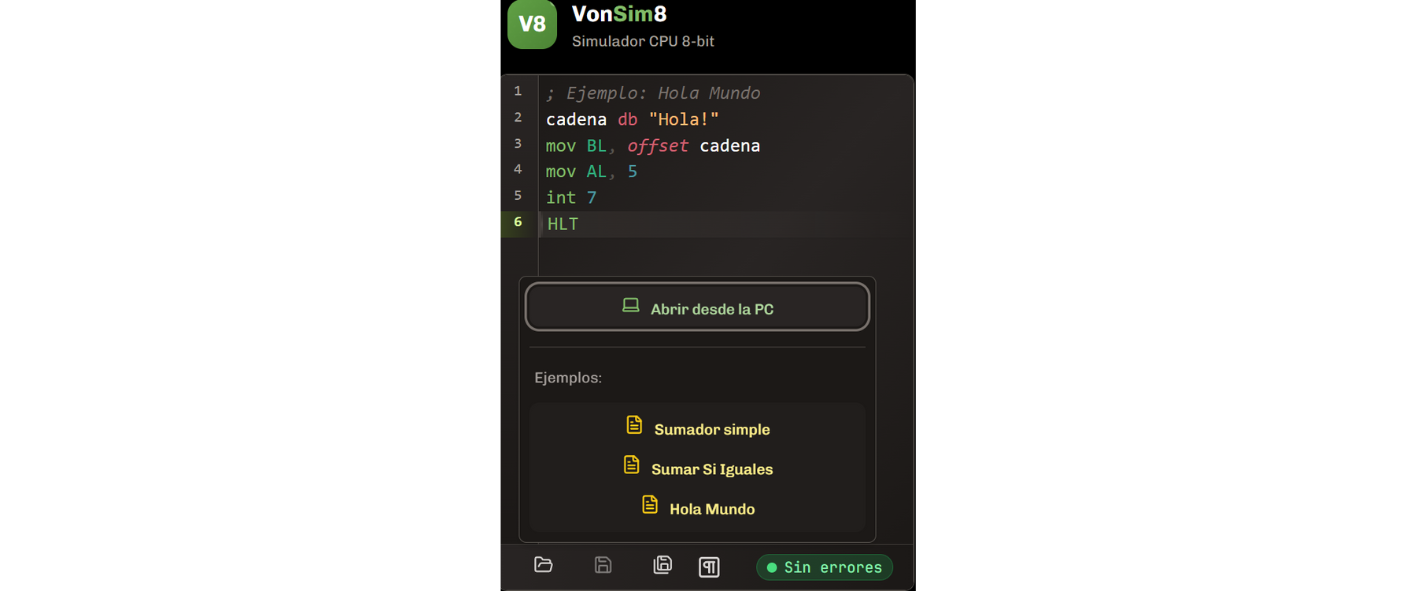
\includegraphics[width=0.9\linewidth]{images/editor} 

}

\caption{Editor ensamblador}\label{fig:editor}
\end{figure}

\begin{enumerate}
\def\labelenumi{\arabic{enumi}.}
\setcounter{enumi}{2}
\tightlist
\item
  \textbf{Repertorio reducido de instrucciones con activación progresiva:}
  Se selecciona un subconjunto esencial del conjunto de instrucciones x86, el cual se habilita en etapas secuenciales del proceso de enseñanza, en correspondencia con el avance de los contenidos curriculares. Esta decisión se fundamenta en principios de la psicología cognitiva que sugieren que la introducción escalonada de contenidos técnicos mejora la retención y reduce la sobrecarga cognitiva \protect\hyperlink{ref-nationalacademies2018how}{{[}70{]}}. Esta estrategia también se encuentra respaldada por autores como Hasan \protect\hyperlink{ref-hasan_survey_2012}{{[}18{]}}, Null y Lobur \protect\hyperlink{ref-null_essentials_2023}{{[}33{]}}, y Stallings \protect\hyperlink{ref-stallings_computer_2021}{{[}20{]}}, quienes proponen abordajes similares en la enseñanza de arquitecturas complejas.
\end{enumerate}

\begin{table}[!h]
\centering
\caption{\label{tab:activacionprogresiva}Activación progresiva del repertorio de instrucciones}
\centering
\resizebox{\ifdim\width>\linewidth\linewidth\else\width\fi}{!}{
\fontsize{10}{12}\selectfont
\begin{tabular}[t]{>{\centering\arraybackslash}p{2cm}|>{\centering\arraybackslash}p{4cm}>{\centering\arraybackslash}p{6cm}}
\toprule
\multicolumn{1}{>{\centering\arraybackslash}p{2cm}}{\cellcolor[HTML]{D3D3D3}{\textbf{Fase}}} & \multicolumn{1}{>{\centering\arraybackslash}p{4cm}}{\cellcolor[HTML]{D3D3D3}{\textbf{Instrucciones activadas}}} & \multicolumn{1}{>{\centering\arraybackslash}p{6cm}}{\cellcolor[HTML]{D3D3D3}{\textbf{Objetivo didáctico}}}\\
\midrule
\textbf{Inicial} & MOV, ADD, SUB, HLT & Comprensión del ciclo de instrucción básico\\
\addlinespace[10pt]
\textbf{Intermedia} & CMP, JMP, Jxx & Introducción a control de flujo\\
\addlinespace[10pt]
\textbf{Avanzada} & CALL, RET, INT, IRET, CLI, STI, IN, OUT & Manejo de periféricos e interrupciones\\
\addlinespace[10pt]
\bottomrule
\end{tabular}}
\end{table}

Este enfoque promueve el desarrollo progresivo de competencias, al mitigar la sobrecarga cognitiva que implicaría abordar de forma prematura el repertorio completo de instrucciones. La activación progresiva del repertorio se fundamenta en teorías de aprendizaje que sugieren que la exposición gradual a nuevos conceptos mejora la comprensión y retención \protect\hyperlink{ref-sweller2010cognitive}{{[}71{]}}. Además, esta estrategia se alinea con las recomendaciones de autores como Null y Lobur \protect\hyperlink{ref-null_essentials_2023}{{[}33{]}}, quienes destacan la importancia de introducir los conceptos de forma escalonada para facilitar el aprendizaje efectivo.

\begin{enumerate}
\def\labelenumi{\arabic{enumi}.}
\setcounter{enumi}{3}
\tightlist
\item
  \textbf{Simulación visual e interactiva de micropasos de instrucciones:}
  Se implementa una visualización interactiva del flujo de datos basada en el modelo de Nivel de Transferencia entre Registros (Register Transfer Level, RTL). Este enfoque permite representar con precisión el desplazamiento de datos entre registros, buses y unidades funcionales del procesador, así como las señales de control involucradas en cada fase del ciclo de instrucción \protect\hyperlink{ref-harris2015digital}{{[}32{]}}, \protect\hyperlink{ref-ASMVisualizer2025}{{[}72{]}}. Stallings \protect\hyperlink{ref-stallings_computer_2021}{{[}20{]}} propone utilizar el modelo RTL para representar el ciclo de instrucción, desde la captura (fetch) hasta la ejecución (execute), facilitando la visualización del recorrido de datos y señales de control en cada etapa del proceso.
  Como complemento a la descripción anterior, la Figura \ref{fig:cicloinstruccion} muestra un ciclo de instrucción típico utilizando la operación \texttt{MOV\ AL,\ BL}. En la etapa de captación (\emph{fetch}), la dirección de la instrucción se carga desde el registro \texttt{IP} al \texttt{MAR}, y el contenido de la memoria se transfiere al \texttt{MBR} y luego al \texttt{IR} . En la etapa de ejecución (\emph{execute}), los datos se mueven desde el registro \texttt{BL} al registro \texttt{AL}.
\end{enumerate}

\begin{figure}

{\centering 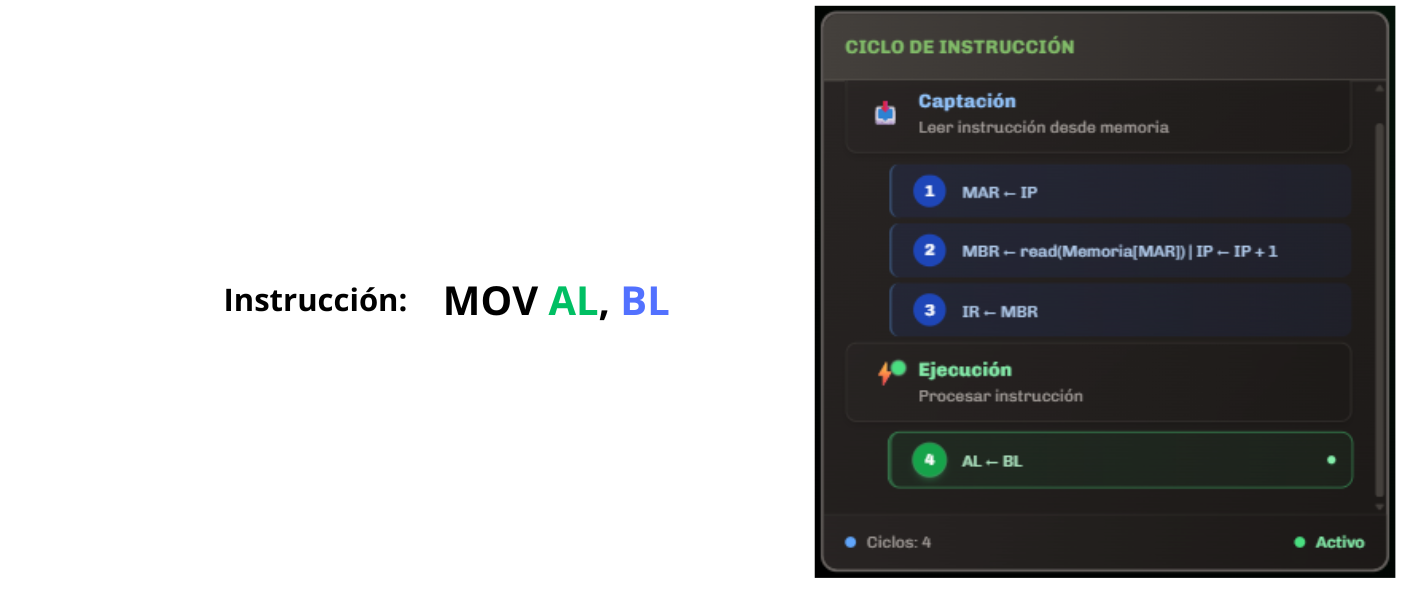
\includegraphics[width=0.85\linewidth]{images/cicloinstruccion} 

}

\caption{Ciclo de instrucción: captación y ejecución}\label{fig:cicloinstruccion}
\end{figure}

\begin{enumerate}
\def\labelenumi{\arabic{enumi}.}
\setcounter{enumi}{4}
\tightlist
\item
  \textbf{Gestión básica de interrupciones y periféricos:}
  Incluir un vector de interrupciones predefinido que simule eventos externos, como la entrada de datos mediante teclado o la salida de información a través de un monitor. El vector de interrupciones predefinido permite simular eventos externos, como la entrada de datos mediante teclado. Por ejemplo, al recibir una interrupción de teclado, el simulador activa la señal \texttt{INTR}, detiene la ejecución actual y transfiere el control a la rutina de tratamiento de interrupciones correspondiente. Desde el punto de vista pedagógico, esta funcionalidad ofrece al estudiante la posibilidad de explorar de manera interactiva conceptos clave como la asincronía, el manejo de eventos y la interrupción del flujo secuencial, todos ellos característicos del diseño de arquitecturas modernas y fundamentales para el entendimiento de sistemas reales. Su inclusión se alinea con las recomendaciones de autores como Null y Lobur \protect\hyperlink{ref-null_essentials_2023}{{[}33{]}}, quienes destacan el valor de abordar estos conceptos en etapas tempranas de la formación. Además, se incorpora un módulo genérico de entrada/salida programada (Programmed Input/Output, PIO), que actúa como interfaz entre la CPU y los dispositivos periféricos. Este módulo permite simular operaciones mediante instrucciones como IN y OUT, facilitando la interacción del estudiante con dispositivos representados gráficamente, como interruptores y teclas. De esta forma, se promueve una comprensión más tangible de los mecanismos subyacentes al intercambio de información entre el procesador y los dispositivos externos.
\end{enumerate}

\begin{figure}

{\centering 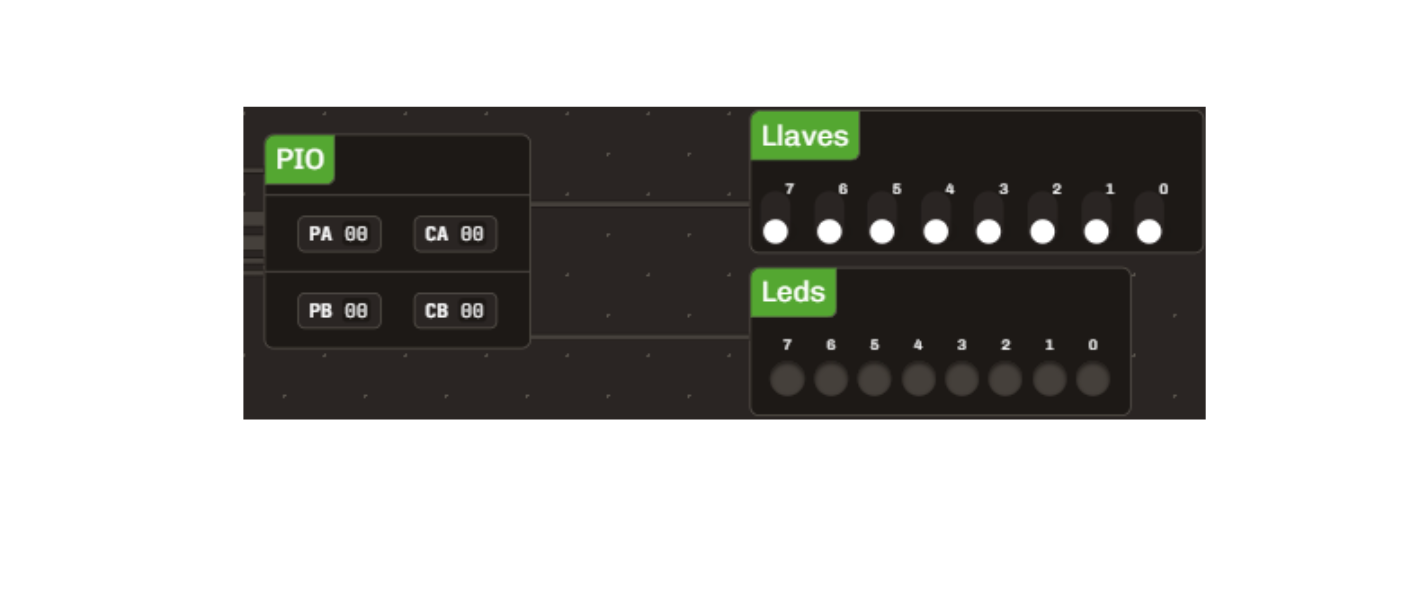
\includegraphics[width=0.85\linewidth]{images/perifericos} 

}

\caption{Módulo genérico de entrada/salida programada}\label{fig:perifericos}
\end{figure}

\begin{enumerate}
\def\labelenumi{\arabic{enumi}.}
\setcounter{enumi}{5}
\tightlist
\item
  \textbf{Métricas de rendimiento:}
  Incluir indicadores clave como tiempo de ciclo, tiempo de CPU y ciclos por instrucción (CPI), generados automáticamente a partir de la ejecución de los programas. Asimismo, se permite configurar la frecuencia del CPU dentro de un rango de valores (1--10 Hz). Estos indicadores permiten al estudiante analizar cuantitativamente la eficiencia en la ejecución de un programa, facilitando comparaciones entre diferentes implementaciones. Su inclusión apunta a fortalecer la comprensión de aspectos clave del rendimiento del procesador, promoviendo una formación integral que contemple tanto aspectos funcionales como métricos del comportamiento del sistema \protect\hyperlink{ref-hennessy2017computer}{{[}19{]}}.
\end{enumerate}

\begin{figure}

{\centering 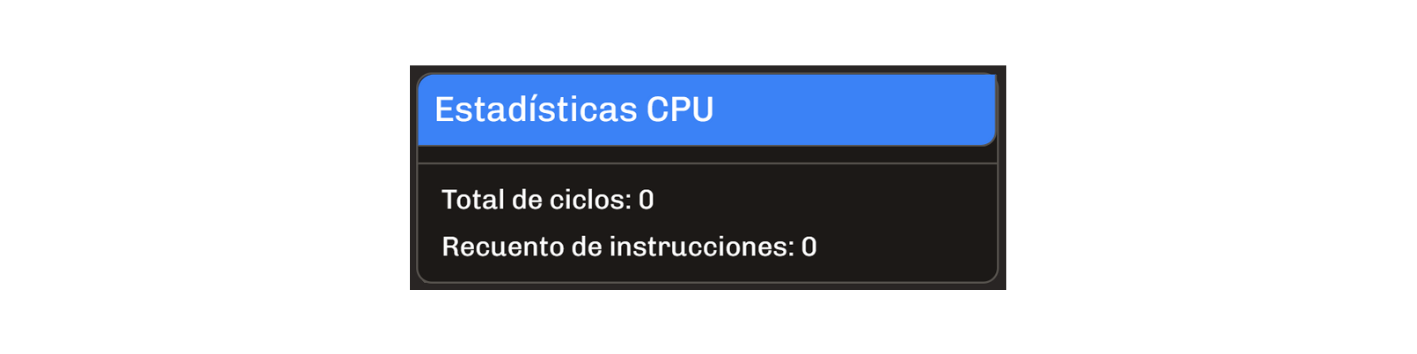
\includegraphics[width=0.85\linewidth]{images/metricas} 

}

\caption{Métricas de rendimiento}\label{fig:metricas}
\end{figure}

\begin{enumerate}
\def\labelenumi{\arabic{enumi}.}
\setcounter{enumi}{6}
\tightlist
\item
  \textbf{Documentación y recursos de apoyo:}
  Proporcionar documentación clara y accesible que explique el funcionamiento del simulador, sus componentes y las instrucciones disponibles. Esta documentación debe incluir ejemplos prácticos, guías de uso y recursos adicionales para facilitar la comprensión y el aprendizaje autónomo. La inclusión de tutoriales interactivos y ejemplos prácticos es fundamental para guiar al estudiante en el uso efectivo del simulador, promoviendo un aprendizaje activo y reflexivo \protect\hyperlink{ref-bonwell1991active}{{[}73{]}}.
\end{enumerate}

\begin{figure}

{\centering 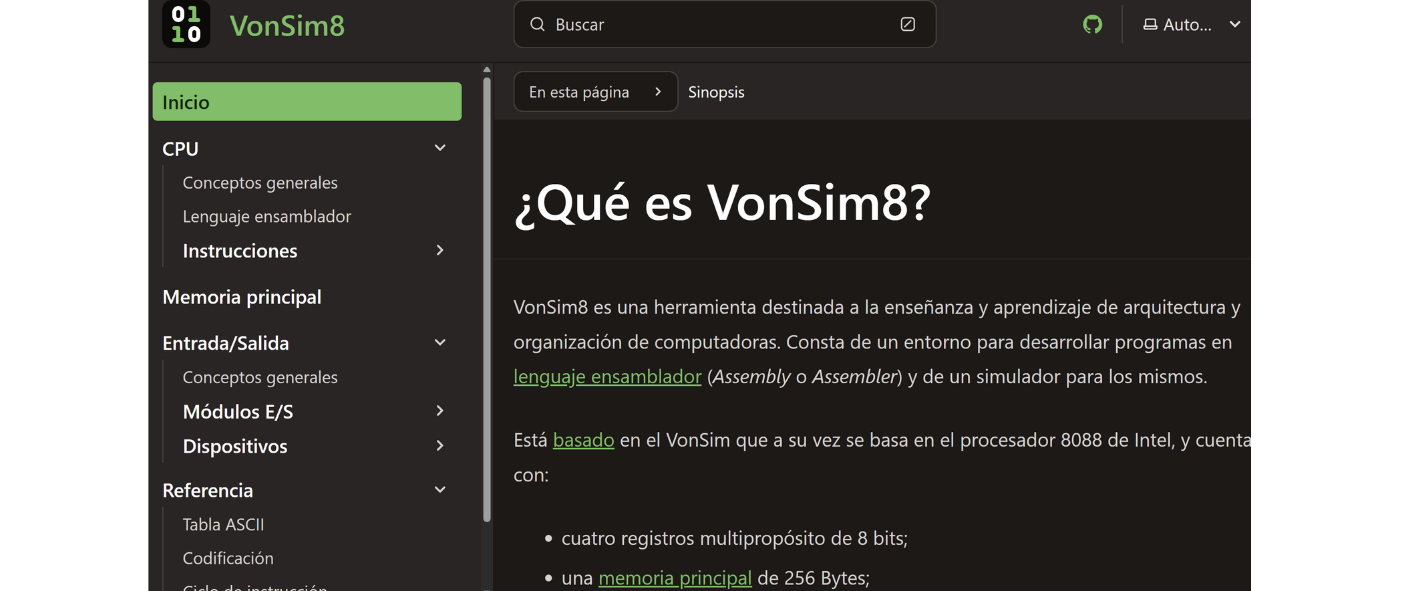
\includegraphics[width=0.9\linewidth]{images/documentacion} 

}

\caption{Documentación on line}\label{fig:documentacion}
\end{figure}

En conjunto, estos requisitos constituyen la base del diseño del simulador, garantizando tanto su pertinencia pedagógica como su viabilidad técnica. Su formulación responde a la necesidad de contar con un recurso didáctico que facilite la enseñanza y el aprendizaje de la arquitectura x86, integrando aspectos visuales, interactivos y de análisis del rendimiento. La Tabla \ref{tab:requisitosresumen} presenta un resumen de los principales requisitos funcionales, junto con su fundamentación pedagógica y técnica.

\begin{table}[!h]
\centering
\caption{\label{tab:requisitosresumen}Resumen de requisitos funcionales y su fundamentación pedagógica}
\centering
\resizebox{\ifdim\width>\linewidth\linewidth\else\width\fi}{!}{
\fontsize{10}{12}\selectfont
\begin{tabular}[t]{>{\centering\arraybackslash}p{5cm}|>{\centering\arraybackslash}p{8cm}}
\toprule
\multicolumn{1}{>{\centering\arraybackslash}p{5cm}}{\cellcolor[HTML]{D3D3D3}{\textbf{Requisito}}} & \multicolumn{1}{>{\centering\arraybackslash}p{8cm}}{\cellcolor[HTML]{D3D3D3}{\textbf{Fundamento pedagógico / técnico}}}\\
\midrule
\textbf{Visualización de estructura general} & Facilita comprensión sistémica mediante representaciones gráficas de hardware.\\
\addlinespace[10pt]
\textbf{Soporte para programas en ensamblador} & Desarrolla competencias en trazado y depuración de lenguaje ensamblador; mejora usabilidad.\\
\addlinespace[10pt]
\textbf{Repertorio reducido y activación progresiva} & Disminuye sobrecarga cognitiva al introducir instrucciones de manera escalonada.\\
\addlinespace[10pt]
\textbf{Simulación visual de micropasos (RTL)} & Permite comprender el flujo interno de datos y señales de control durante el ciclo de instrucción.\\
\addlinespace[10pt]
\textbf{Gestión de interrupciones y periféricos} & Simula asincronía y manejo de eventos, favoreciendo la comprensión de sistemas reales.\\
\addlinespace[10pt]
\addlinespace
\textbf{Métricas de rendimiento} & Promueve análisis cuantitativo de eficiencia (CPI, ciclos, tiempo de CPU).\\
\addlinespace[10pt]
\textbf{Documentación y recursos de apoyo} & Fomenta aprendizaje autónomo y activo mediante guías, tutoriales y ejemplos.\\
\addlinespace[10pt]
\bottomrule
\end{tabular}}
\end{table}

La definición de los requisitos funcionales y pedagógicos permitió identificar la necesidad de simplificar la arquitectura x86 para adaptarla a los objetivos educativos. Esta simplificación asegura que los estudiantes puedan concentrarse en los conceptos fundamentales sin verse abrumados por la complejidad técnica. A continuación, se detalla la justificación de esta decisión.

\hypertarget{justificaciuxf3n-pedaguxf3gica-de-la-arquitectura-simplificada}{%
\section{Justificación pedagógica de la arquitectura Simplificada}\label{justificaciuxf3n-pedaguxf3gica-de-la-arquitectura-simplificada}}

A partir de los requisitos funcionales detallados anteriormente, se realizó un proceso colaborativo de análisis con docentes\footnote{Docentes: Marcelo A. Colombani y Amalia G. Delduca} de la asignatura Arquitectura de Computadoras. Su experiencia permitió identificar los elementos de la arquitectura x86 que debían representarse, simplificarse o adaptarse según los objetivos pedagógicos del simulador. Como resultado, se optó por una arquitectura simplificada de 8 bits, cuya elección se justifica por su valor didáctico: reduce la complejidad del modelo sin comprometer la enseñanza de conceptos esenciales como el ciclo de instrucciones, la manipulación de registros o la gestión de interrupciones. Esta simplificación permite representar procesos clave con mayor claridad y menor carga cognitiva, favoreciendo la comprensión de los estudiantes en las etapas iniciales del aprendizaje.

La arquitectura x86 se distingue por su elevada complejidad, derivada de su extenso repertorio de instrucciones y sus múltiples características avanzadas. En respuesta, el diseño del simulador se fundamenta en tres principios pedagógicos centrales:

\begin{itemize}
\tightlist
\item
  \textbf{Reducir la carga cognitiva}: simplificar el repertorio y los componentes permite a los estudiantes enfocarse en los principios fundamentales.\\
\item
  \textbf{Aprendizaje progresivo}: se adopta un enfoque escalonado, comenzando con un modelo simple y avanzando hacia representaciones más completas de x86.\\
\item
  \textbf{Claridad pedagógica}: las prácticas resultan manejables en términos de tiempo y esfuerzo, favoreciendo un aprendizaje activo y centrado en la resolución progresiva de problemas.
\end{itemize}

En este marco, el diseño del simulador contribuye a:

\begin{itemize}
\tightlist
\item
  \textbf{Comprensión fundamental}: los estudiantes pueden concentrarse en el ciclo de instrucciones, la interacción de componentes y el flujo básico de datos.\\
\item
  \textbf{Análisis crítico}: comparar el modelo simplificado con la arquitectura x86 real favorece un aprendizaje más reflexivo y profundo.\\
\item
  \textbf{Experimentación práctica}: proporciona un entorno accesible para explorar conceptos y corregir errores.
\end{itemize}

Diversos autores como Patterson \& Hennessy \protect\hyperlink{ref-hennessy2017computer}{{[}19{]}}, Tanenbaum \protect\hyperlink{ref-tanenbaum_structured_2016}{{[}28{]}} y Null \protect\hyperlink{ref-null_essentials_2023}{{[}33{]}} coinciden en que el uso de arquitecturas simplificadas, como las de 8 bits, permite a los estudiantes centrarse en los fundamentos de la arquitectura de computadoras sin verse abrumados por la complejidad técnica de arquitecturas reales. Este enfoque hace posible observar la transferencia de datos entre registros y la activación de señales de control en cada etapa, facilitando la comprensión del funcionamiento interno del procesador.

El modelo propuesto se inspira en los principios de la arquitectura x86 \protect\hyperlink{ref-intel_microarchitecture_2021}{{[}45{]}}, pero implementa un repertorio reducido de instrucciones en una arquitectura de 8 bits. Esta elección responde a criterios pedagógicos: simplifica el modelo sin sacrificar los principios esenciales del repertorio x86, y facilita una comprensión progresiva de sus componentes \protect\hyperlink{ref-patt2019introduction}{{[}74{]}}, \protect\hyperlink{ref-majid1999design}{{[}75{]}}, \protect\hyperlink{ref-morlan_sap1_2021}{{[}76{]}}, \protect\hyperlink{ref-Guald_2015_thesis}{{[}77{]}}, \protect\hyperlink{ref-silber_tinycpu}{{[}78{]}}.

Aunque la simplificación a 8 bits reduce la fidelidad del modelo respecto a la arquitectura x86 real, esta decisión permite a los estudiantes concentrarse en los principios fundamentales, como el ciclo de instrucciones y la interacción entre registros. Para abordar esta limitación, el simulador incluye funcionalidades avanzadas que pueden activarse progresivamente, como la gestión de interrupciones y el repertorio completo de instrucciones.

En síntesis, la definición de estos requisitos integra aspectos funcionales, pedagógicos y técnicos en una herramienta que no solo simula el comportamiento del sistema, sino que además facilita activamente los procesos de enseñanza y aprendizaje en arquitectura de computadoras. La combinación entre visualización, ejecución progresiva y análisis de rendimiento ofrece un entorno didáctico rico que responde tanto a las necesidades del aula como a los desafíos de la disciplina.

\hypertarget{introducciuxf3n-a-vonsim}{%
\section{Introducción a VonSim}\label{introducciuxf3n-a-vonsim}}

VonSim\footnote{VonSim: \url{https://vonsim.github.io/}} \protect\hyperlink{ref-vonsim}{{[}79{]}} es una herramienta diseñada específicamente para la enseñanza y el aprendizaje de la arquitectura y organización de computadoras, que sirvió de referencia por su enfoque educativo e interfaz intuitiva. A partir de esta herramienta se desarrolló VonSim8\footnote{VonSim8: \url{https://ruiz-jose.github.io/VonSim8/}}, adaptado para operar con registros y memoria de 8\,bits, y diseñado para favorecer el aprendizaje progresivo.

VonSim ofrece una arquitectura detallada con un amplio repertorio de instrucciones y componentes. Aunque esta riqueza funcional es valiosa, puede resultar abrumadora para estudiantes en etapas iniciales. Por esta razón, VonSim8 implementa una simplificación estratégica para reducir la carga cognitiva en los primeros niveles de aprendizaje, promoviendo una asimilación progresiva de los conceptos fundamentales de la arquitectura de computadoras. A partir de esta base, se introdujeron diversas modificaciones en los componentes, instrucciones y funcionalidades del simulador, priorizando aquellos aspectos conceptuales que se abordan en el programa de la asignatura.

Las siguientes características posicionan a VonSim como una solución educativa integral:

\begin{enumerate}
\def\labelenumi{\arabic{enumi}.}
\item
  \textbf{Entorno integrado de desarrollo y simulación:} incluye un editor de código ensamblador con resaltado de sintaxis y un simulador para la ejecución de programas, facilitando el aprendizaje práctico. \protect\hyperlink{ref-vonsim}{{[}79{]}}.
\item
  \textbf{Fundamento en arquitectura real:} basado en el procesador Intel 8088, ofrece una referencia histórica y técnicamente relevante. \protect\hyperlink{ref-intel8086manual}{{[}51{]}}.
\item
  \textbf{Componentes esenciales para el estudio:} incorpora cuatro registros multipropósito de 16 bits, memoria principal de 32 kB, bus de direcciones de 16 bits y bus de datos de 8 bits, entre otros. \protect\hyperlink{ref-stallings_computer_2021}{{[}20{]}}.
\item
  \textbf{Gestión completa de interrupciones:} Implementa tanto interrupciones por software (entrada/salida de datos) como interrupciones por hardware mediante un controlador de interrupciones programable (PIC), cubriendo aspectos fundamentales de la operación del sistema \protect\hyperlink{ref-hennessy2017computer}{{[}19{]}}.
\item
  \textbf{Simulación de periféricos:} incorpora dispositivos como reloj, llaves, luces e impresora, inspirados en los especificados por la familia iAPX 88 de Intel, permitiendo simular interacciones complejas con el sistema.
\item
  \textbf{Enfoque pedagógico mediante simplificaciones estratégicas:} no pretende ser un emulador fiel del 8088, sino una herramienta educativa que implementa simplificaciones deliberadas (repertorio de instrucciones reducido y codificación simplificada) para facilitar la comprensión en contextos educativos \protect\hyperlink{ref-patt2019introduction}{{[}74{]}}.
\item
  \textbf{Desarrollo académico especializado:} fue creado por Facundo Quiroga, Manuel Bustos Berrondo y Juan Martín Seery, con la colaboración de Andoni Zubimendi y César Estrebou, específicamente para las cátedras de Organización de Computadoras y Arquitectura de Computadoras de la Facultad de Informática de la Universidad Nacional de La Plata, garantizando su alineación con objetivos curriculares específicos.
\item
  \textbf{Fundamento en experiencia previa:} se basa en el simulador MSX88, desarrollado en 1988 por Rubén de Diego Martínez para la Universidad Politécnica de Madrid, aprovechando décadas de experiencia acumulada en simuladores educativos.
\item
  \textbf{Accesibilidad y sostenibilidad:} distribuido bajo licencia GNU Affero General Public License v3.0 con código fuente disponible en GitHub, y documentación bajo licencia CC BY-SA 4.0, facilitando su estudio, modificación y mejora continua \protect\hyperlink{ref-opensource_licensing_2024}{{[}80{]}}.
\end{enumerate}

\hypertarget{stack-tecnoluxf3gico}{%
\subsubsection{Stack tecnológico}\label{stack-tecnoluxf3gico}}

El proyecto VonSim está desarrollado íntegramente en TypeScript, lo que permite aprovechar el tipado estático, lograr mayor robustez del código y contar con mejor soporte para autocompletado y detección temprana de errores durante el desarrollo.

La organización del código sigue la estructura de un monorepositorio, compuesto por diversos paquetes especializados que cumplen funciones específicas:

\begin{itemize}
\tightlist
\item
  vonsim/assembler: ensamblador que traduce el código en lenguaje ensamblador a binario ejecutable.
\item
  vonsim/simulator: motor que ejecuta los programas ensamblados.
\item
  vonsim/app: aplicación web que proporciona la interfaz gráfica de usuario e integra el simulador.
\item
  vonsim/common: utilidades compartidas entre los distintos módulos.
\item
  eslint-config-vonsim: paquete para la configuración de reglas de estilo y buenas prácticas mediante ESLint.
\item
  vonsim/scripts y vonsim/tsconfig: paquetes de soporte con scripts de desarrollo y configuraciones específicas para TypeScript.
\item
  vonsim/docs: módulo destinado a la gestión de la documentación del proyecto.
\end{itemize}

Para el desarrollo y la ejecución del proyecto se utilizan herramientas modernas como Node.js v22 y el gestor de paquetes pnpm v10. Asimismo, el repositorio incluye una serie de scripts predefinidos para facilitar las tareas de instalación, compilación y despliegue: pnpm install, pnpm dev, pnpm docs:dev y pnpm build.

\hypertarget{estructura-del-vonsim8}{%
\section{Estructura del VonSim8}\label{estructura-del-vonsim8}}

En esta sección se describe la estructura del simulador VonSim8. El diseño de los registros se concibió con un propósito pedagógico: facilitar la comprensión de los modos de direccionamiento y del ciclo de instrucción, elementos fundamentales en el estudio de la Arquitectura de Computadoras \protect\hyperlink{ref-stallings_computer_2021}{{[}20{]}}. En la tabla \ref{tab:estructuravonsim8} se describen los componentes principales del simulador, junto con sus características y funcionalidades específicas. Esta tabla proporciona una visión general de la arquitectura del simulador, destacando los elementos clave que componen su estructura:

\begin{table}[!h]
\centering
\caption{\label{tab:estructuravonsim8}Estructura VonSim8: componentes principales y características}
\centering
\resizebox{\ifdim\width>\linewidth\linewidth\else\width\fi}{!}{
\fontsize{10}{12}\selectfont
\begin{tabular}[t]{>{\raggedright\arraybackslash}p{4cm}|p{12cm}}
\toprule
\multicolumn{1}{>{\centering\arraybackslash}p{4cm}}{\cellcolor[HTML]{D3D3D3}{\textbf{Componente}}} & \multicolumn{1}{>{\centering\arraybackslash}p{12cm}}{\cellcolor[HTML]{D3D3D3}{\textbf{Características}}}\\
\midrule
\textbf{Arquitectura} & Von Neumann: memoria compartida para datos e instrucciones.\\
\addlinespace[10pt]
\textbf{Registros generales} & 4 registros de propósito general de 8 bits (`AL`, `BL`, `CL`, `DL`).\\
\addlinespace[10pt]
\textbf{Registros específicos} & 6 registros de propósito específico:\begin{itemize} \item IP (Instruction Pointer) \item IR (Instruction Register) \item SP (Stack Pointer) \item Flags (registro de estado) \item MAR (Memory Address Register) \item MBR (Memory Buffer Register)\end{itemize}\\
\addlinespace[10pt]
\textbf{Acceso a registros} & Los registros de propósito general pueden ser accedidos y modificados por el programador. Los específicos son gestionados por la CPU.\\
\addlinespace[10pt]
\textbf{Memoria} & Memoria principal de 256 bytes, direccionada por un bus de direcciones de 8 bits. Cada posición almacena un byte. La memoria se organiza en celdas de 16 bytes, con dirección inicial `0x00` y final `0xFF`.\\
\addlinespace[10pt]
\addlinespace
\textbf{Puertos} & Puertos de la CPU:\begin{itemize} \item Bus de direcciones de 8 bits (MAR) \item Bus de datos de 8 bits (MBR) \item Señal de lectura (rd) y escritura (wr), cada una de 1 bit \item Señal IO/M (1 bit) para distinguir acceso a memoria o E/S \item Señal de petición de interrupción (INTR, 1 bit) \item Señal de reconocimiento de interrupción (INTA, 1 bit)\end{itemize}\\
\addlinespace[10pt]
\bottomrule
\end{tabular}}
\end{table}

Entre los registros específicos, no accesibles directamente por el programador, se incluyen los siguientes:

\begin{itemize}
\tightlist
\item
  \textbf{\texttt{SP} (\emph{Stack Pointer})}: Responsable de la gestión de la pila, permitiendo el seguimiento de las direcciones de memoria asociadas a las operaciones de apilamiento y desapilamiento.\\
\item
  \textbf{\texttt{Flags} (\emph{Flags Register})}: Registro que almacena las banderas de estado, utilizadas para reflejar el resultado de operaciones aritméticas y lógicas, así como para controlar el flujo del programa.\\
\item
  \textbf{\texttt{IP} (\emph{Instruction Pointer})}: Contiene la dirección de memoria de la próxima instrucción a ejecutar, asegurando la secuenciación correcta del programa.\\
\item
  \textbf{\texttt{IR} (\emph{Instruction Register})}: Almacena el byte correspondiente a la instrucción que está siendo decodificada y ejecutada en el momento.
\end{itemize}

Adicionalmente, se disponen de dos registros esenciales para la transferencia de datos entre la CPU y la memoria principal:

\begin{itemize}
\tightlist
\item
  \textbf{\texttt{MAR} (\emph{Memory Address Register})}: Encargado de almacenar las direcciones de memoria que se desean acceder.\\
\item
  \textbf{\texttt{MBR} (\emph{Memory Buffer Register})}: Almacena temporalmente el byte de datos que se transfiere hacia o desde la memoria principal a través del bus de datos.
\end{itemize}

Adicionalmente, se incluyen dos registros auxiliares: \texttt{ri}, destinado al almacenamiento temporal de direcciones, e \texttt{id}, orientado al almacenamiento temporal de datos. Estos registros cumplen una función de apoyo en la ejecución de instrucciones.

\hypertarget{unidad-de-control}{%
\subsection{Unidad de Control}\label{unidad-de-control}}

La unidad de control es responsable de coordinar todas las operaciones de la CPU. Se encarga de:

\begin{itemize}
\tightlist
\item
  \textbf{Decodificación de instrucciones}: Interpreta el código de operación de cada instrucción.
\item
  \textbf{Generación de señales de control}: Activa las señales necesarias para ejecutar microoperaciones.
\item
  \textbf{Secuenciación}: Controla el orden de ejecución de las operaciones.
\end{itemize}

\hypertarget{memoria-de-control}{%
\subsubsection{Memoria de Control}\label{memoria-de-control}}

La memoria de control almacena microinstrucciones que guían la ejecución de cada instrucción en el simulador. Una representación visual de esta memoria, organizada en filas (microinstrucciones) y columnas (microoperaciones y señales de control), facilita la comprensión del papel que desempeña en la coordinación de la unidad de control \protect\hyperlink{ref-stallings_computer_2021}{{[}20{]}}.

\hypertarget{secuenciador}{%
\subsubsection{Secuenciador}\label{secuenciador}}

El secuenciador complementa la memoria de control mostrando cómo se controla la secuencia de microoperaciones y las señales de control generadas en cada fase del ciclo de instrucción.

\hypertarget{unidad-aritmuxe9tico-luxf3gica-alu}{%
\subsection{Unidad Aritmético-Lógica (ALU)}\label{unidad-aritmuxe9tico-luxf3gica-alu}}

La ALU (\emph{Arithmetic Logic Unit}) realiza operaciones aritméticas y lógicas, como \texttt{ADD} y \texttt{SUB}. Durante el ciclo de instrucción, la unidad de control genera señales específicas que activan las operaciones de la ALU. Por ejemplo, al ejecutar una instrucción \texttt{ADD}, la unidad de control activa las señales necesarias para transferir los operandos desde los registros hacia la ALU y almacenar el resultado en el registro de destino. Todas estas operaciones modifican el registro \texttt{Flags}.

\hypertarget{registro-de-banderas-flags}{%
\subsubsection{Registro de Banderas (Flags)}\label{registro-de-banderas-flags}}

El registro de banderas \texttt{Flags} almacena las banderas de estado que reflejan el resultado de operaciones aritméticas y lógicas. Por ejemplo, después de una operación de suma, la bandera \texttt{Z} (Zero) se activa si el resultado es cero, lo que permite al procesador tomar decisiones condicionales basadas en este estado.

\begin{table}[!h]
\centering
\caption{\label{tab:tflags}Registro Flags: descripción de las banderas}
\centering
\resizebox{\ifdim\width>\linewidth\linewidth\else\width\fi}{!}{
\fontsize{10}{12}\selectfont
\begin{tabular}[t]{>{\centering\arraybackslash}p{2cm}|>{\centering\arraybackslash}p{3cm}>{\raggedright\arraybackslash}p{7cm}}
\toprule
\multicolumn{1}{>{\centering\arraybackslash}p{2cm}}{\cellcolor[HTML]{D3D3D3}{\textbf{Bit N°}}} & \multicolumn{1}{>{\centering\arraybackslash}p{3cm}}{\cellcolor[HTML]{D3D3D3}{\textbf{Abreviatura}}} & \multicolumn{1}{>{\centering\arraybackslash}p{7cm}}{\cellcolor[HTML]{D3D3D3}{\textbf{Descripción}}}\\
\midrule
\textbf{0} & Z & Flag de cero (Zero)\\
\addlinespace[10pt]
\textbf{1} & C & Flag de acarreo (Carry)\\
\addlinespace[10pt]
\textbf{2} & O & Flag de desbordamiento (Overflow)\\
\addlinespace[10pt]
\textbf{3} & S & Flag de signo (Sign)\\
\addlinespace[10pt]
\textbf{4} & I & Flag de interrupción (Interrupt)\\
\addlinespace[10pt]
\bottomrule
\end{tabular}}
\end{table}

Los bits restantes del registro Flags se encuentran reservados para posibles extensiones del simulador y no están en uso en la versión actual.

\hypertarget{memoria-principal}{%
\subsection{Memoria principal}\label{memoria-principal}}

La memoria principal se modela como una matriz de 16×16 expresada en formato hexadecimal, lo que permite almacenar hasta 256 bytes de datos. Esta capacidad resulta suficiente para la mayoría de los programas de ejemplo utilizados en el curso, y su diseño simplificado facilita la comprensión de los conceptos fundamentales asociados a la memoria principal en una computadora.

\begin{figure}

{\centering 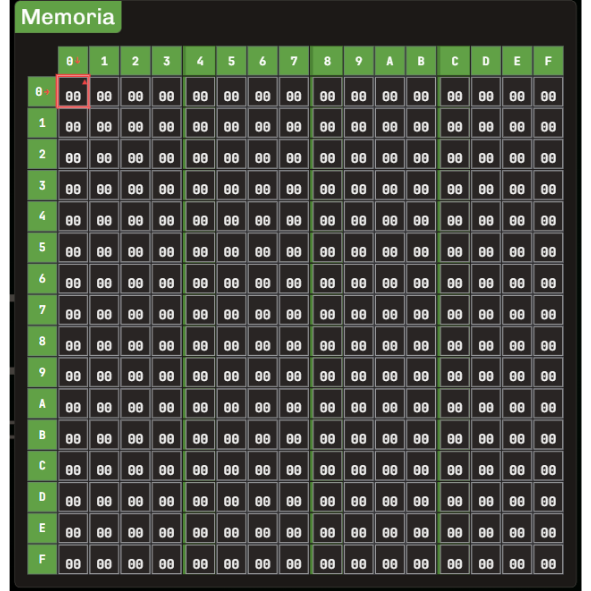
\includegraphics[width=0.85\linewidth]{images/memoria} 

}

\caption{Memoria principal}\label{fig:memoria}
\end{figure}

\hypertarget{buses-y-multiplexores}{%
\subsection{Buses y multiplexores}\label{buses-y-multiplexores}}

Los buses de datos, direcciones y control se modelan como un conjunto de líneas que permiten la comunicación entre los distintos componentes del sistema. Estos buses resultan esenciales para el intercambio de información entre la CPU, la memoria y los dispositivos de entrada/salida. Además, su diseño modular favorece la posibilidad de expansión en futuras versiones del simulador.

\begin{figure}

{\centering 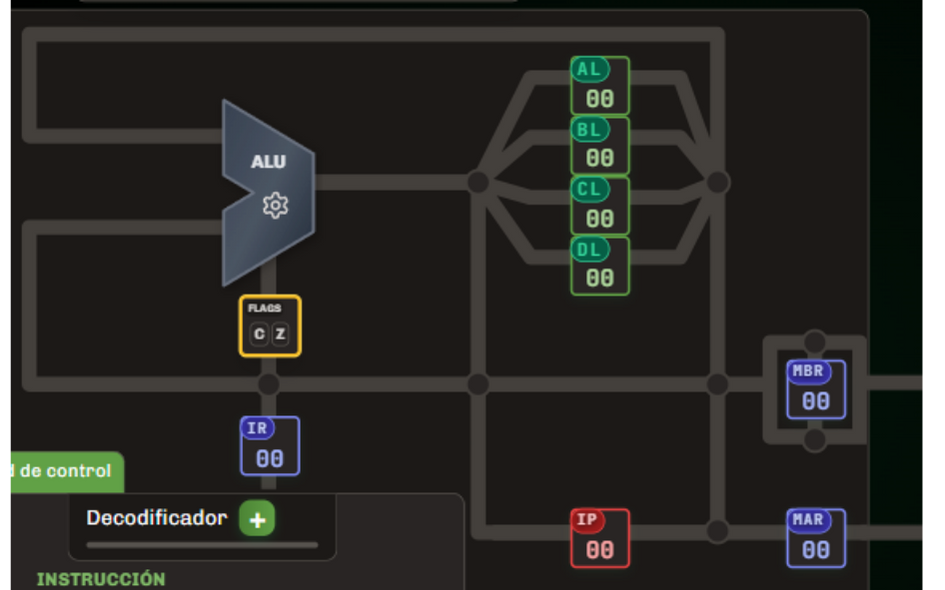
\includegraphics[width=0.85\linewidth]{images/buses} 

}

\caption{Buses}\label{fig:buses}
\end{figure}

Dentro de los buses internos de la CPU se incluyen representaciones gráficas de multiplexores, componentes digitales esenciales que permiten seleccionar entre múltiples fuentes de datos o direcciones durante el ciclo de instrucción. Los multiplexores dirigen las señales hacia los registros y la ALU (Unidad Aritmético-Lógica), facilitando el flujo de datos dentro del procesador. Un multiplexor (MUX) funciona como un conmutador digital que conecta datos de una de n fuentes a la salida. Están dotados de entradas de control capaces de seleccionar una y solo una de las entradas de datos para permitir su transmisión desde la entrada seleccionada hacia dicha salida \protect\hyperlink{ref-mano2017digital}{{[}81{]}}.

\hypertarget{adaptaciones-y-mejoras-en-vonsim8}{%
\section{Adaptaciones y mejoras en VonSim8}\label{adaptaciones-y-mejoras-en-vonsim8}}

Si bien VonSim ofrece una base sólida para la enseñanza de arquitectura de computadoras, su complejidad funcional puede resultar abrumadora para estudiantes en etapas iniciales. Por esta razón, se implementaron modificaciones estratégicas en VonSim8, orientadas a simplificar el modelo y alinearlo con los objetivos pedagógicos de la asignatura. A continuación, se describen las principales mejoras realizadas.

Las modificaciones implementadas se alinean con los contenidos curriculares de la asignatura y están fundamentadas en los principios del aprendizaje activo \protect\hyperlink{ref-bonwell1991active}{{[}73{]}}.

\begin{enumerate}
\def\labelenumi{\arabic{enumi}.}
\tightlist
\item
  Simplificación del repertorio instruccional para una introducción gradual;
\item
  Reducción a registros y memoria de 8\,bits, coherente con la escala de enseñanza;
\item
  Interfaz gráfica esquemática que muestra el flujo de ejecución;
\item
  Funciones interactivas para observar explícitamente el ciclo de instrucción y la interacción de componentes.
\end{enumerate}

A continuacion se detallan los cambios más relevantes implementados en VonSim8, junto con capturas de pantalla que ilustran las modificaciones realizadas:

En el registro Flags de VonSim se ocultaron inicialmente las banderas O (overflow) y S (signo), dado que en los primeros ejercicios de ensamblador solo se emplean números enteros positivos. No obstante, estas banderas pueden habilitarse posteriormente desde el menú de configuración del simulador, conforme se abordan ejercicios de mayor complejidad.

\begin{figure}

{\centering 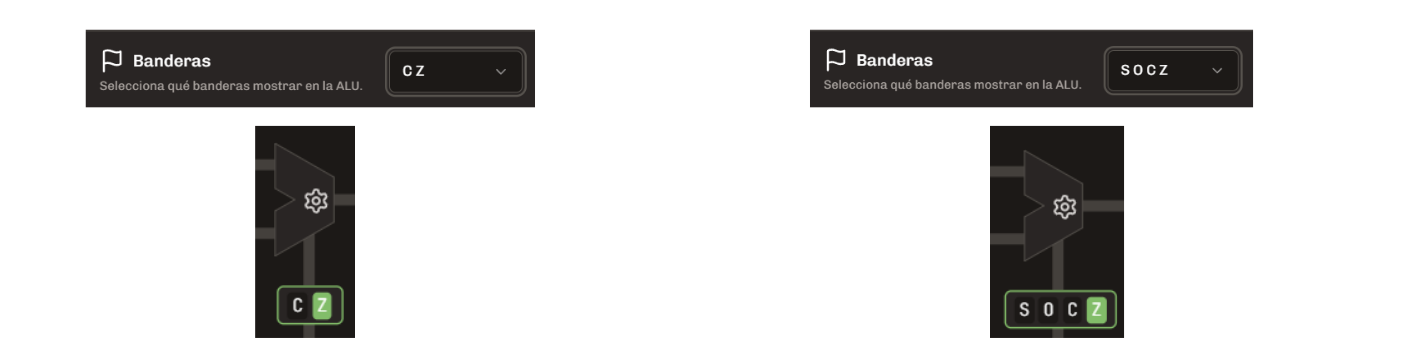
\includegraphics[width=0.85\linewidth]{images/flags} 

}

\caption{Registro Flags}\label{fig:banderas}
\end{figure}

El flag de interrupcion I solo se muestra cuando el programa lo requiere, por ejemplo, al ejecutar una instrucción de interrupción como \texttt{INT} o \texttt{IRET}. Esto permite a los estudiantes observar cómo se activa y desactiva este flag en función de las operaciones realizadas.

\begin{figure}

{\centering 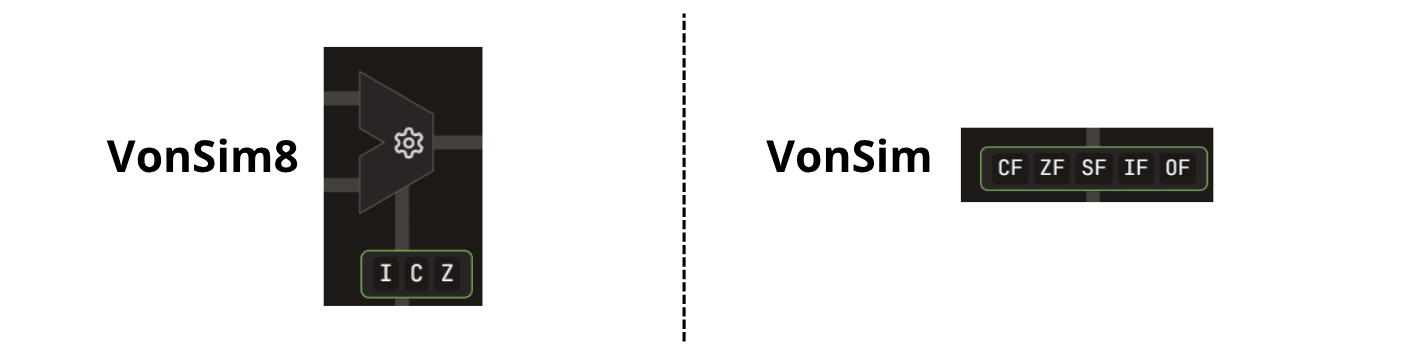
\includegraphics[width=0.85\linewidth]{images/flagi} 

}

\caption{Registro de estado I}\label{fig:banderaI}
\end{figure}

Se modificó el menú de los controles del simulador.

\begin{figure}

{\centering 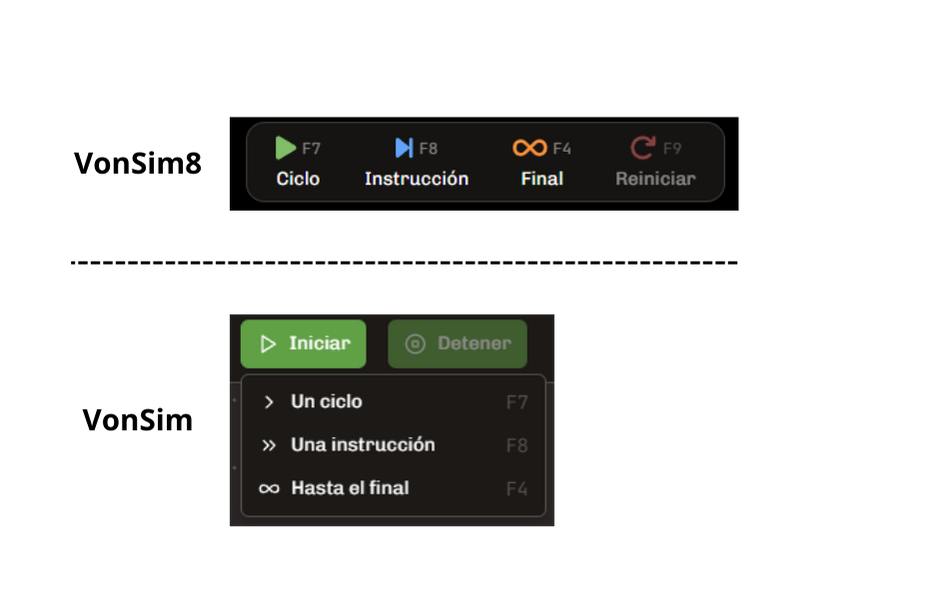
\includegraphics[width=0.85\linewidth]{images/controles} 

}

\caption{Controles del simulador}\label{fig:controles}
\end{figure}

En lugar de utilizar registros de 16 bits completos, se emplea únicamente la parte baja de cada registro, lo que simplifica tanto la representación como la manipulación de los datos. Esta decisión responde a la necesidad de reducir la complejidad del modelo, facilitando así la comprensión de los conceptos fundamentales de la arquitectura de computadoras. Además, se ha unificado el criterio de diseño de los registros: todos cuentan ahora con una entrada y una salida independientes, lo que permite visualizar de manera más clara la transferencia de datos entre los registros y la Unidad Aritmético-Lógica (ALU). Esta modificación resulta esencial para comprender el flujo de datos durante el ciclo de instrucción y la interacción entre los distintos componentes del procesador.

\begin{figure}

{\centering 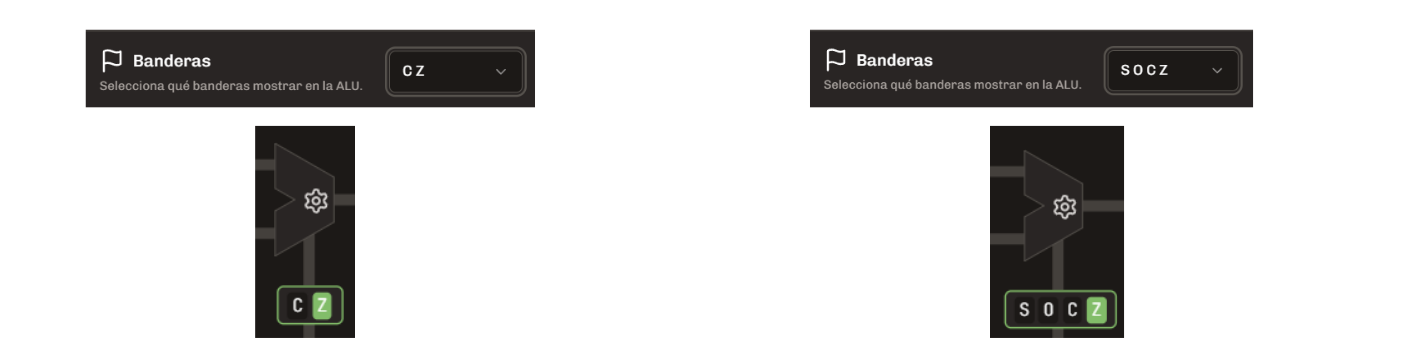
\includegraphics[width=0.85\linewidth]{images/registros} 

}

\caption{Registro de 8 bits}\label{fig:registros}
\end{figure}

La eliminación de los registros temporales \texttt{left}, \texttt{right} y \texttt{result} en la ALU responde a la necesidad de simplificar el flujo de datos y reducir la carga cognitiva de los estudiantes. En lugar de utilizar registros intermedios, el simulador muestra directamente las operaciones realizadas en los operandos, lo que facilita la comprensión del proceso aritmético y lógico.

\begin{figure}

{\centering 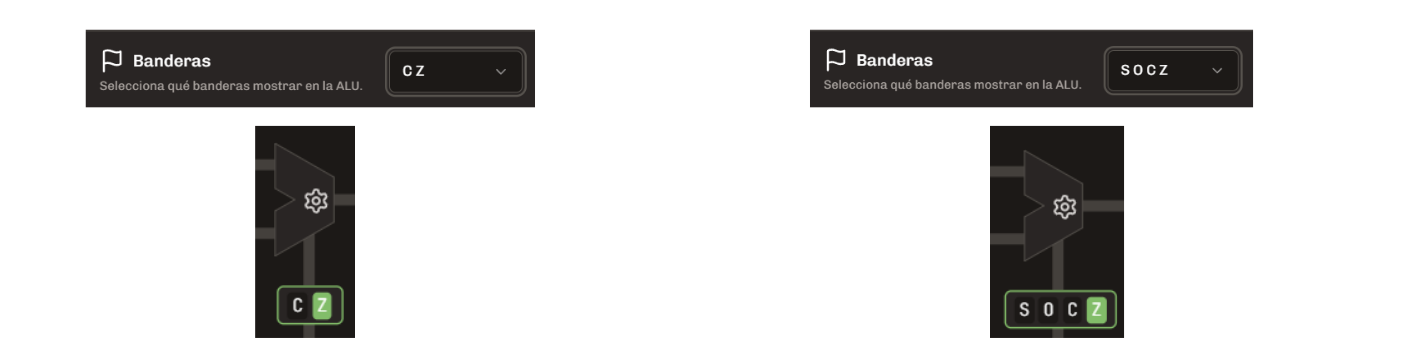
\includegraphics[width=0.85\linewidth]{images/leftrigth} 

}

\caption{Eliminación registro temporales left, right y result}\label{fig:leftrigth}
\end{figure}

Los registros \texttt{SP}, \texttt{ri} e \texttt{id} se mantienen ocultos y solo se habilitan automáticamente cuando una instrucción requiere su utilización.

\begin{figure}

{\centering 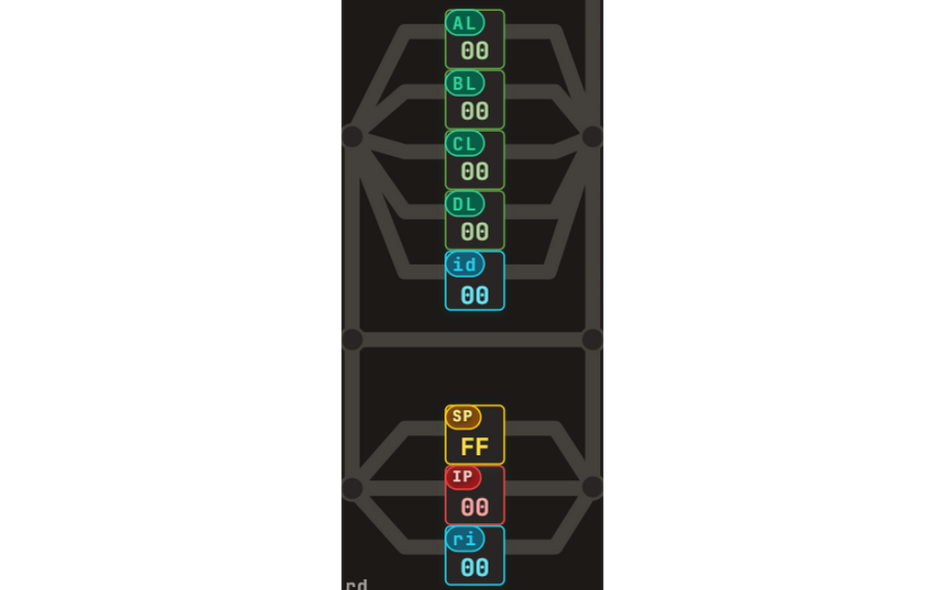
\includegraphics[width=0.85\linewidth]{images/idrisp} 

}

\caption{Registro SP, id y ri}\label{fig:idrisp}
\end{figure}

La memoria principal se modela como una matriz de 16×16 expresada en hexadecimal, lo que permite almacenar hasta 256 bytes de datos.

\begin{figure}

{\centering 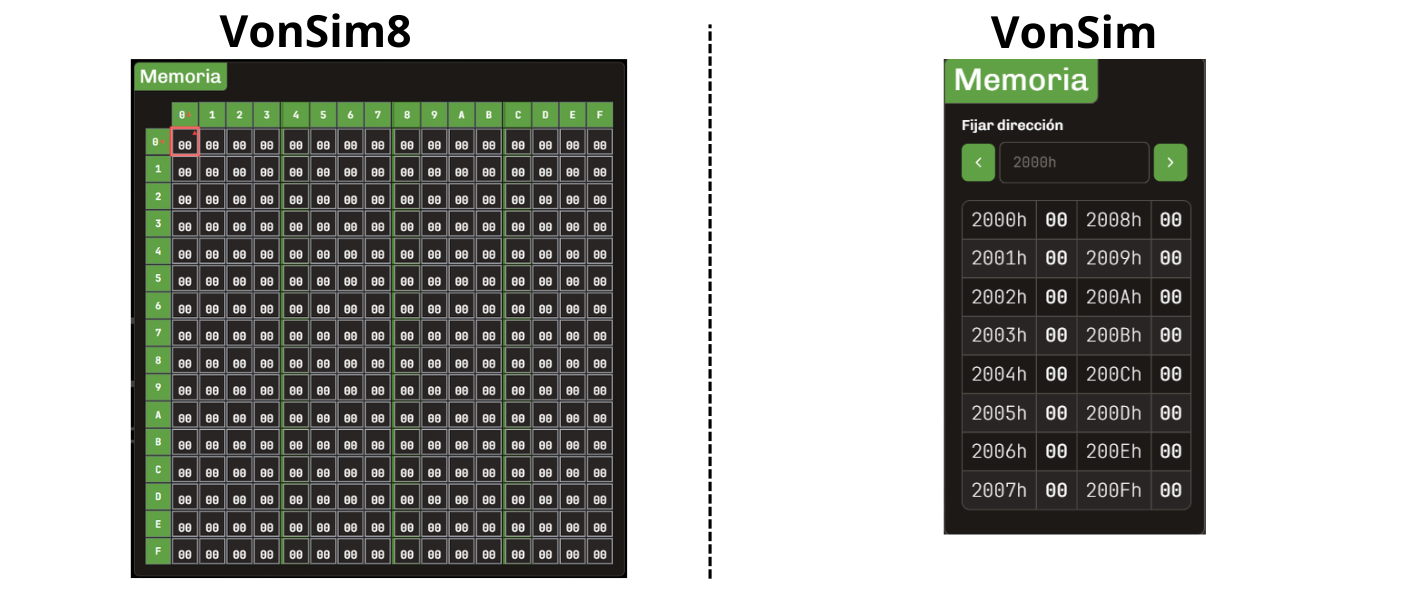
\includegraphics[width=0.85\linewidth]{images/memoriacomp} 

}

\caption{Memoria principal}\label{fig:memoriacomp}
\end{figure}

Resalto de la direccion de memoria apuntada por el registro IP en memoria y también resalta la dirección de memoria apuntada por el registro SP.

\begin{figure}

{\centering 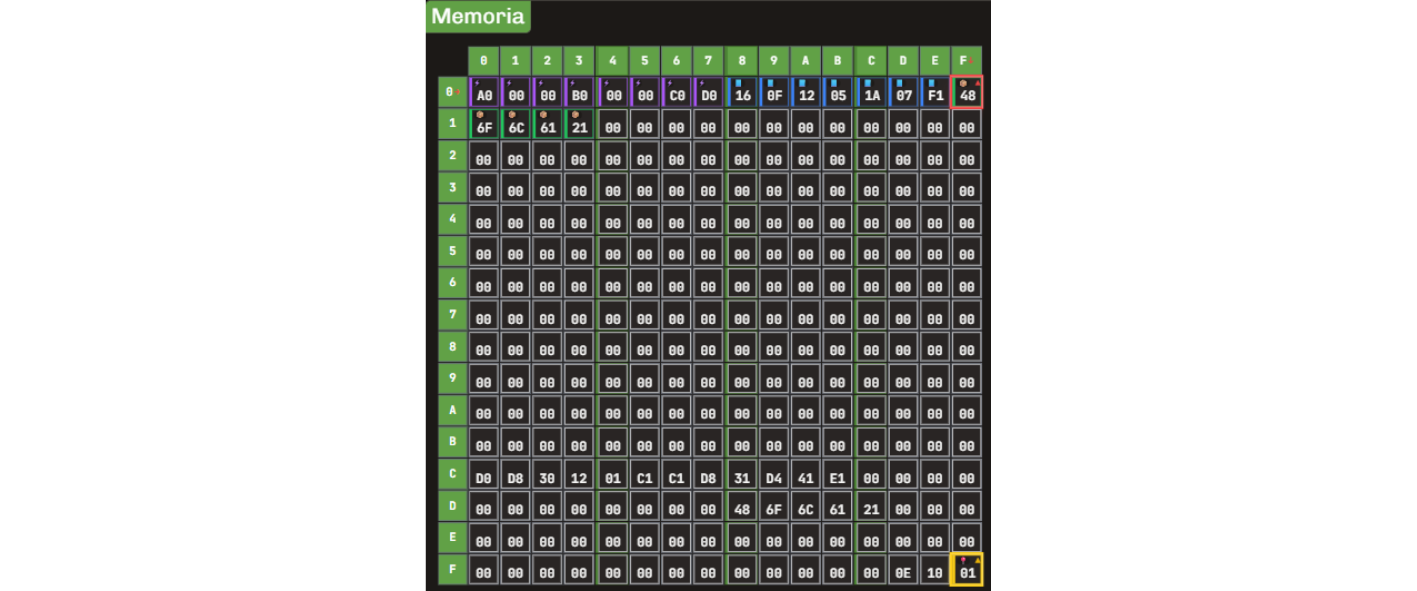
\includegraphics[width=0.85\linewidth]{images/resaltadoipsp} 

}

\caption{Resaltado registro IP y registro SP}\label{fig:resaltadoip}
\end{figure}

Se resalta en color violeta en la memoria principal el espacio destinado al vector de interrupciones en el VonSim8 es de 8 posiciones de memoria desde \texttt{0x00} a \texttt{0x07}:

\begin{figure}

{\centering 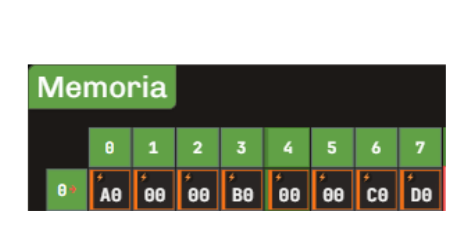
\includegraphics[width=0.85\linewidth]{images/resaltadoint} 

}

\caption{Resaltado vector de interrupciones}\label{fig:resaltadointsp}
\end{figure}

Para determinar la dirección de la rutina de tratamiento de interrupción en VonSim, es necesario multiplicar el número de interrupción por 4, ya que cada dirección de rutina ocupa 4 bytes. En cambio, en VonSim8 no es necesario realizar esta multiplicación, dado que cada dirección de rutina de interrupción corresponde a un solo byte. Por lo tanto, la interrupcion \texttt{INT\ 0} se encuentra en la direccion \texttt{0x00}, la interrupcion \texttt{INT\ 6} en la direccion \texttt{0x06}, y así sucesivamente.

Se incorporó un visor de instrucciones y datos del programa en memoria, que permite visualizar la instrucción, el tamaño en bytes que ocupa en memoria y la etiqueta asociada a los datos.

\begin{figure}

{\centering 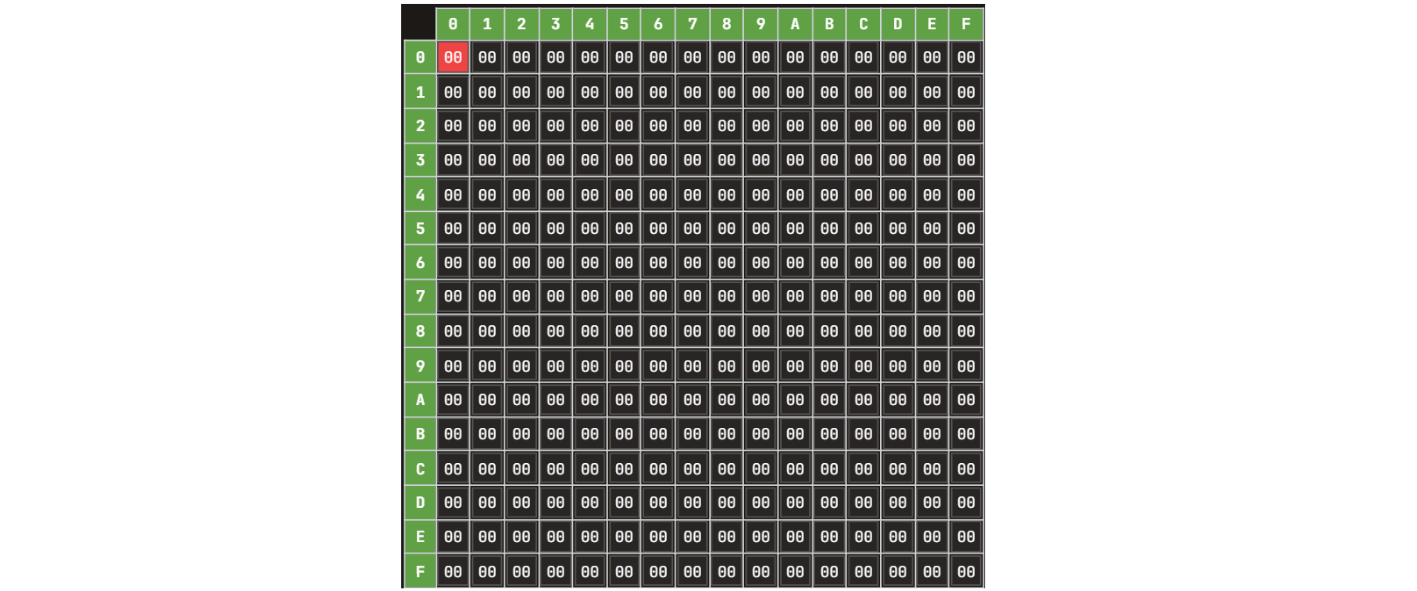
\includegraphics[width=0.85\linewidth]{images/visorprog} 

}

\caption{Visor de instrucciones y datos del programa en memoria}\label{fig:visorprog}
\end{figure}

En VonSim, cuando se escribe un programa en el editor del simulador, es obligatorio que la sección de código inicie con la directiva \texttt{ORG\ 0x2000h} y que termine con la directiva \texttt{END}. Esto se debe a que el simulador comienza a ejecutar la primera instrucción a partir de la dirección de memoria \texttt{0x2000h}. De manera complementaria, los datos del programa suelen cargarse a partir de la dirección \texttt{0x1000h} mediante la directiva \texttt{ORG\ 0x1000h}.

En VonSim8, el uso de la directiva \texttt{ORG} para definir la dirección inicial es opcional. Por defecto, si el programa no incluye esta directiva, la primera instrucción se carga en la dirección \texttt{0x00h}. En caso de contener instrucciones de interrupción (INT), el simulador asigna automáticamente la dirección \texttt{0x08h} como punto de inicio, reservando espacio para el vector de interrupciones.

Por una cuestion de compatibilidad se permite cargar programas de manera similar a VonSim, pero en lugar de cargar el programa en la direccion \texttt{0x2000h} se debe cargar en la \texttt{0x20h}. En este caso, el simulador comienza a ejecutar las instrucciones a partir de la dirección \texttt{0x20h}. Para mantener compatibilidad con VonSim, se conserva esta directiva, permitiendo a los usuarios establecer direcciones personalizadas.

\begin{figure}

{\centering 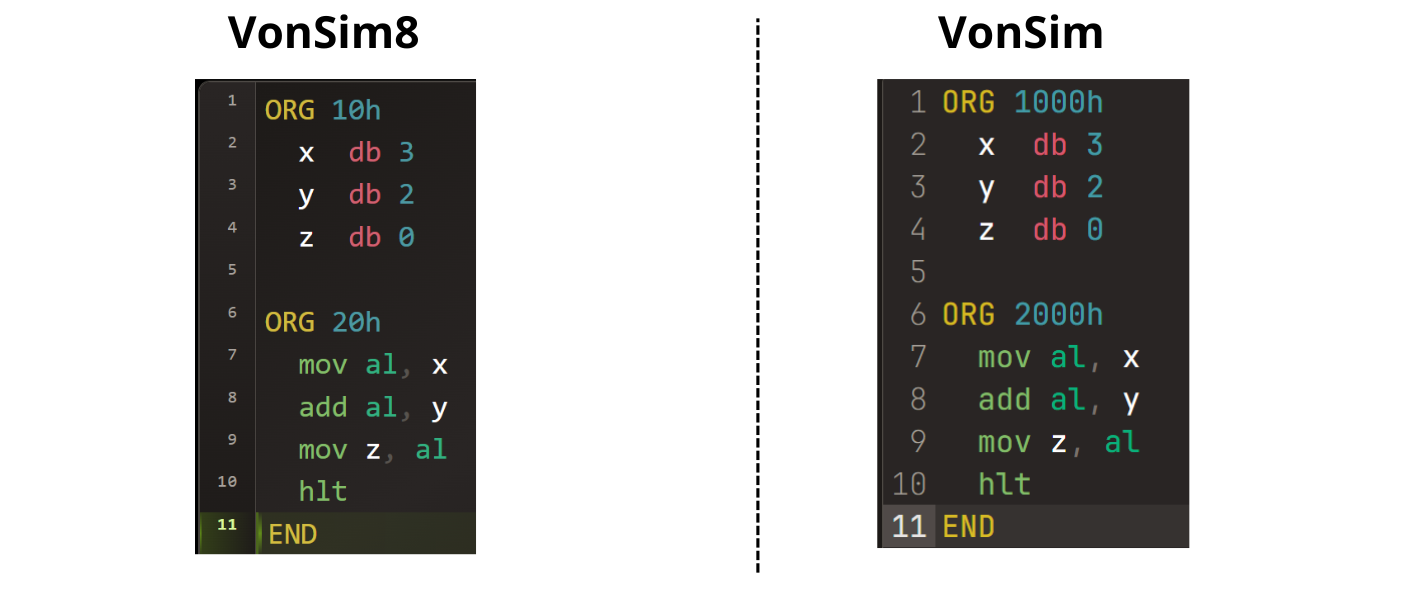
\includegraphics[width=0.85\linewidth]{images/org} 

}

\caption{Compatibilitad directiva ORG y END}\label{fig:org}
\end{figure}

Además, en VonSim8 se incorporó la opción de abrir ejemplos prácticos para que el estudiante pueda experimentar directamente con el simulador. También se desarrolló un tour de aprendizaje que guía al usuario a través de las principales funcionalidades, junto con un centro de aprendizaje que ofrece explicaciones y ejemplos básicos.

\begin{figure}

{\centering 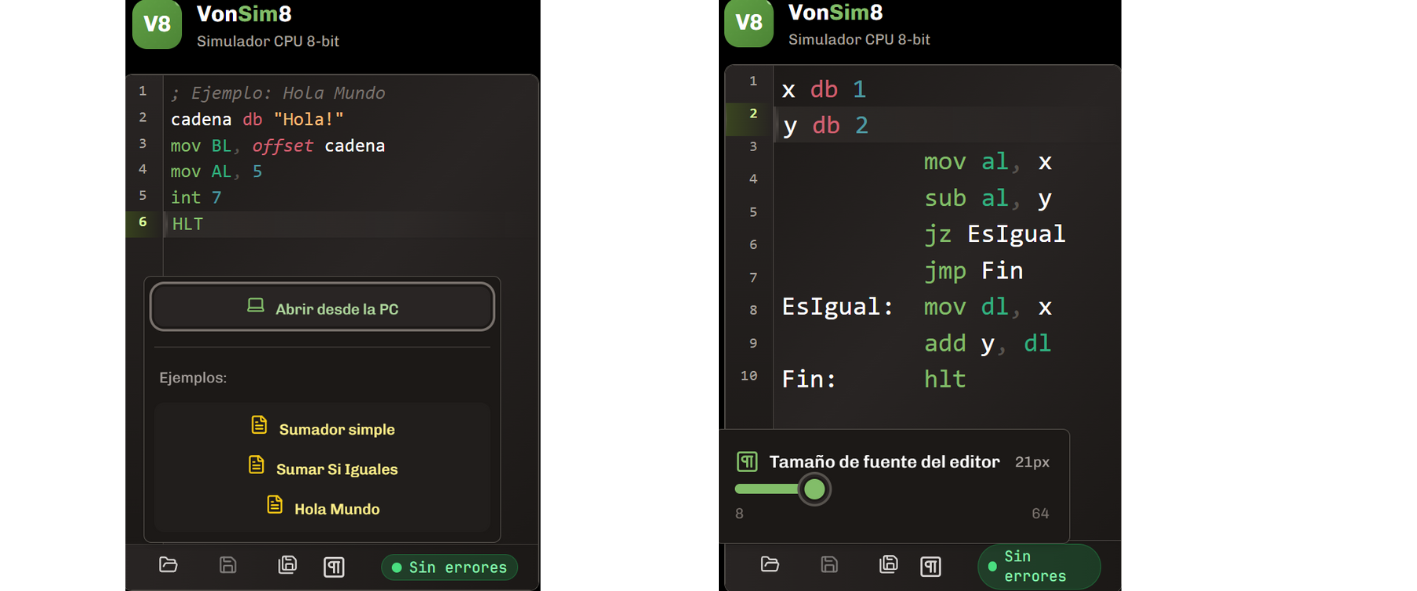
\includegraphics[width=0.85\linewidth]{images/editorfuenteejemplo} 

}

\caption{Editor con ampliación de fuente y ejemplos}\label{fig:editorvonsim}
\end{figure}

Se ha mejorado el diseño de la unidad de control incorporando, dentro del decodificador, una memoria de control y un secuenciador. Estos componentes permiten representar el ciclo de instrucción de manera detallada, mostrando las microoperaciones y las señales de control generadas en cada etapa del proceso.

\begin{figure}

{\centering 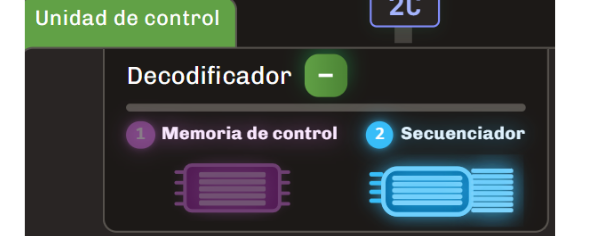
\includegraphics[width=0.85\linewidth]{images/decodificador} 

}

\caption{Decodificador en VonSim8}\label{fig:decodificador}
\end{figure}

Con el fin de facilitar el aprendizaje del simulador VonSim8 se implementó un tour de aprendizaje que guía a los usuarios a través de las características y funcionalidades del simulador. También se incluye un centro de aprendizaje con explicación de ejemplos básicos.

\begin{figure}

{\centering 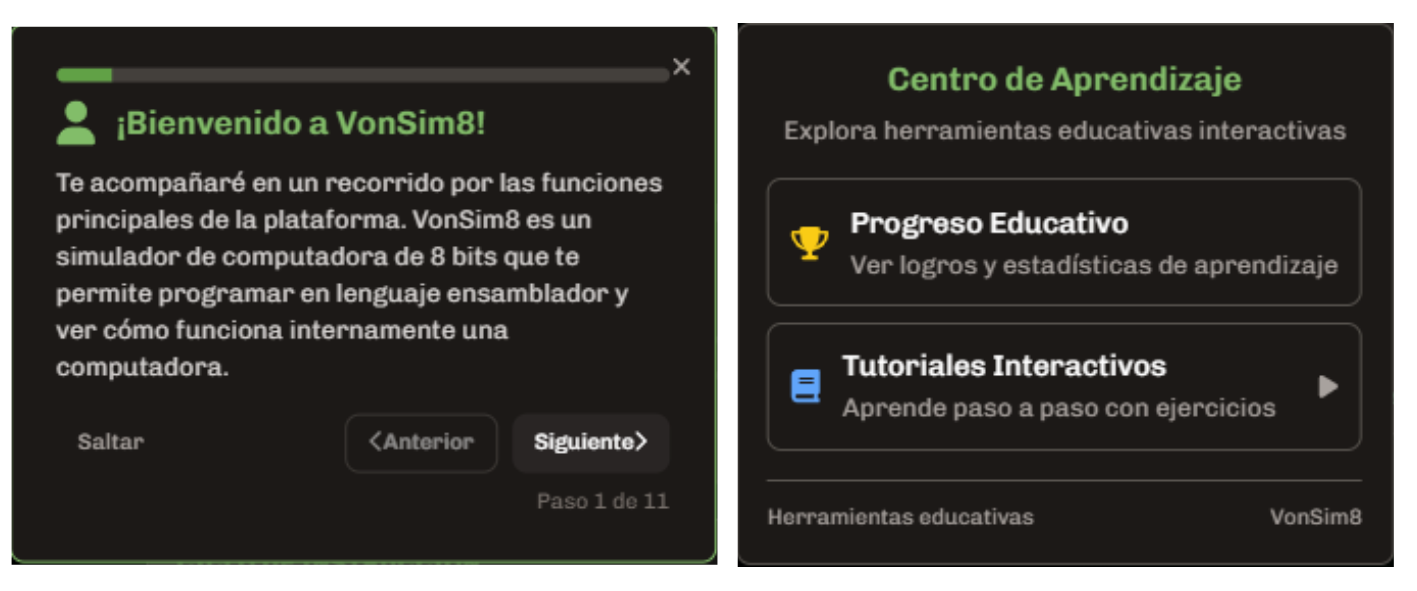
\includegraphics[width=0.85\linewidth]{images/tour} 

}

\caption{Tour de aprendizaje en VonSim8}\label{fig:tour}
\end{figure}

A fin de sintetizar las diferencias más relevantes entre VonSim y VonSim8, se presenta la siguiente tabla comparativa. Esta permite visualizar de manera inmediata los cambios introducidos en el diseño y su impacto en la enseñanza de los conceptos fundamentales de arquitectura de computadoras.

\begin{table}[!h]
\centering
\caption{\label{tab:comparativavonsim}Comparativa de características entre VonSim y VonSim8}
\centering
\resizebox{\ifdim\width>\linewidth\linewidth\else\width\fi}{!}{
\fontsize{10}{12}\selectfont
\begin{tabular}[t]{>{\raggedright\arraybackslash}p{5cm}|>{\raggedright\arraybackslash}p{7cm}>{\raggedright\arraybackslash}p{8cm}}
\toprule
\multicolumn{1}{>{\centering\arraybackslash}p{5cm}}{\cellcolor[HTML]{D3D3D3}{\textbf{Característica}}} & \multicolumn{1}{>{\centering\arraybackslash}p{7cm}}{\cellcolor[HTML]{D3D3D3}{\textbf{VonSim}}} & \multicolumn{1}{>{\centering\arraybackslash}p{8cm}}{\cellcolor[HTML]{D3D3D3}{\textbf{VonSim8}}}\\
\midrule
\textbf{Registros} & Registros de 16 bits (AX, BX, CX, DX) & Registros de 8 bits, con entrada y salida independientes. Registros SP, RI e ID se ocultan y habilitan automáticamente.\\
\addlinespace[10pt]
\textbf{Registro FLAGS} & Incluye todas las banderas del 8088 (O, S, Z, C, etc.) & Se ocultan inicialmente las banderas O (overflow) y S (signo). El flag I (interrupción) se muestra dinámicamente.\\
\addlinespace[10pt]
\textbf{Controles del simulador} & Menú de controles estándar & Menú de controles modificado y adaptado.\\
\addlinespace[10pt]
\textbf{Directiva org} & Obligatoria. El código comienza en `0x2000h` y los datos en `0x1000h`. & Opcional. Por defecto, el código inicia en `0x00h`. Si hay interrupciones, comienza en `0x08h`. Compatible con `org 0x20h`.\\
\addlinespace[10pt]
\textbf{Memoria principal} & 32 KB, organizada en páginas del 8088. & Matriz de 16×16 bytes (256 bytes), expresada en hexadecimal, con resaltado dinámico de IP y SP.\\
\addlinespace[10pt]
\addlinespace
\textbf{Resaltado de IP y SP} & No resalta dinámicamente IP y SP en memoria. & Resalta en memoria la posición apuntada por IP y SP.\\
\addlinespace[10pt]
\textbf{Vector de interrupciones} & Vector de interrupciones ocupa varias posiciones, cada rutina ocupa 4 bytes. & Vector de interrupciones ocupa 8 posiciones (`0x00` a `0x07`), cada rutina ocupa 1 byte.\\
\addlinespace[10pt]
\textbf{Dirección de rutina de interrupción} & Se multiplica el número de interrupción por 4 para obtener la dirección. & La dirección de la rutina de interrupción coincide con el número de interrupción (ej. INT 6 en `0x06`).\\
\addlinespace[10pt]
\textbf{Visor de instrucciones y datos} & No incluye visor detallado de instrucciones y datos. & Incluye visor de instrucciones y datos, mostrando tamaño y etiquetas.\\
\addlinespace[10pt]
\textbf{Temporales de la ALU} & Registros temporales `left`, `right` y `result` visibles. & Eliminados, para simplificar la representación del ciclo de instrucción.\\
\addlinespace[10pt]
\addlinespace
\textbf{Unidad de control} & Decodificador básico sin memoria de control ni secuenciador. & Decodificador mejorado con memoria de control y secuenciador, permite visualizar microoperaciones y señales de control.\\
\addlinespace[10pt]
\textbf{Enfoque pedagógico} & Mayor fidelidad al procesador Intel 8088, con repertorio más amplio. & Simplificación estratégica para reducir carga cognitiva y favorecer aprendizaje progresivo.\\
\addlinespace[10pt]
\textbf{Editor y recursos didácticos} & Editor estándar, sin ampliación de fuente ni tour de aprendizaje. & Editor con ampliación de fuente, ejemplos prácticos, tour de aprendizaje y centro de ayuda.\\
\addlinespace[10pt]
\bottomrule
\end{tabular}}
\end{table}

\hypertarget{repertorio-de-instrucciones-1}{%
\section{Repertorio de instrucciones}\label{repertorio-de-instrucciones-1}}

El simulador VonSim8 implementa un repertorio reducido de instrucciones, diseñado para facilitar la comprensión de los conceptos fundamentales de la arquitectura de computadoras. Este repertorio incluye instrucciones aritméticas, lógicas, de transferencia de datos y control de flujo, lo que facilita que los estudiantes se familiaricen con las operaciones básicas, evitando la complejidad del repertorio completo de instrucciones x86.

El repertorio de instrucciones del simulador fue concebido como una abstracción pedagógica basada en la arquitectura x86, orientada a optimizar los procesos de enseñanza y aprendizaje en el ámbito educativo. En las primeras etapas del curso, se seleccionan únicamente las instrucciones esenciales, lo que permite introducir de forma gradual y accesible los contenidos fundamentales de la asignatura Arquitectura de Computadoras. Este enfoque progresivo facilita la comprensión de los conceptos clave, evitando la complejidad innecesaria que podría dificultar el aprendizaje inicial \protect\hyperlink{ref-hennessy2017computer}{{[}19{]}}, \protect\hyperlink{ref-tanenbaum_structured_2016}{{[}28{]}}. La Tabla \ref{tab:setreducido} presenta un conjunto reducido de instrucciones que abarca las operaciones más relevantes para una etapa introductoria, centradas en la transferencia y procesamiento de datos, así como en el control de flujo. Esta selección estratégica garantiza la accesibilidad de los conceptos básicos de la arquitectura x86 y se ajusta a los objetivos pedagógicos del curso.

Las instrucciones del simulador VonSim8 se dividen en dos categorías principales: las instrucciones de transferencia y procesamiento de datos, y las instrucciones de control de flujo. Las primeras permiten mover datos entre registros y memoria, realizar operaciones aritméticas y lógicas, y manipular el contenido de los registros. Las segundas permiten alterar el flujo de ejecución del programa mediante saltos condicionales e incondicionales, así como la detención del procesador.

Con el objetivo de favorecer el aprendizaje de la programación en ensamblador y la comprensión del ciclo de instrucción, se presenta a continuación un repertorio de instrucciones alineado con el programa de estudio de la asignatura Arquitectura de Computadoras \protect\hyperlink{ref-cd023_25_programa2025}{{[}82{]}}.

\begin{table}[!h]
\centering
\caption{\label{tab:setreducido}Tabla de instrucciones de VonSim8}
\centering
\resizebox{\ifdim\width>\linewidth\linewidth\else\width\fi}{!}{
\fontsize{10}{12}\selectfont
\begin{tabular}[t]{>{\raggedright\arraybackslash}p{6cm}|>{\raggedright\arraybackslash}p{4cm}>{\raggedright\arraybackslash}p{6cm}}
\toprule
\multicolumn{1}{>{\centering\arraybackslash}p{6cm}}{\cellcolor[HTML]{D3D3D3}{\textbf{Instrucciones}}} & \multicolumn{1}{>{\centering\arraybackslash}p{4cm}}{\cellcolor[HTML]{D3D3D3}{\textbf{nemónico}}} & \multicolumn{1}{>{\centering\arraybackslash}p{6cm}}{\cellcolor[HTML]{D3D3D3}{\textbf{Acción}}}\\
\midrule
\textbf{Transferencia de datos} & MOV & Copiar\\
\addlinespace[8pt]
\textbf{Procesamiento de datos} & ADD & Sumar\\
\addlinespace[8pt]
\textbf{} & SUB & Restar\\
\addlinespace[8pt]
\textbf{} & CMP & Comparar\\
\addlinespace[8pt]
\textbf{Control de flujo} & JMP & Salto incondicional\\
\addlinespace[8pt]
\addlinespace
\textbf{} & Jxx & Salto condicional si xx=1\\
\addlinespace[8pt]
\textbf{} & HLT & Detiene CPU\\
\addlinespace[8pt]
\bottomrule
\end{tabular}}
\end{table}

El parámetro \texttt{xx} en las instrucciones \texttt{Jxx} hace referencia a diferentes combinaciones de banderas de estado (flags), tales como cero (Z), acarreo (C), signo (S) y desbordamiento (O). La negación de un flag se indica con la letra N, lo que amplía la flexibilidad de control del flujo de ejecución en programas condicionales.

\begin{table}[!h]
\centering
\caption{\label{tab:saltoscondicionales}Saltos condicionales: instrucciones y condiciones}
\centering
\resizebox{\ifdim\width>\linewidth\linewidth\else\width\fi}{!}{
\fontsize{10}{12}\selectfont
\begin{tabular}[t]{>{\centering\arraybackslash}p{6cm}|>{\centering\arraybackslash}p{6cm}}
\toprule
\multicolumn{1}{>{\centering\arraybackslash}p{6cm}}{\cellcolor[HTML]{D3D3D3}{\textbf{Instrucción}}} & \multicolumn{1}{>{\centering\arraybackslash}p{6cm}}{\cellcolor[HTML]{D3D3D3}{\textbf{Acción}}}\\
\midrule
\textbf{JZ Dirección} & Salta a \_Dirección\_ si Z = 1\\
\addlinespace[8pt]
\textbf{JNZ Dirección} & Salta a \_Dirección\_ si Z = 0\\
\addlinespace[8pt]
\textbf{JC Dirección} & Salta a \_Dirección\_ si C = 1\\
\addlinespace[8pt]
\textbf{JNC Dirección} & Salta a \_Dirección\_ si C = 0\\
\addlinespace[8pt]
\textbf{JS Dirección} & Salta a \_Dirección\_ si S = 1\\
\addlinespace[8pt]
\addlinespace
\textbf{JNS Dirección} & Salta a \_Dirección\_ si S = 0\\
\addlinespace[8pt]
\textbf{JO Dirección} & Salta a \_Dirección\_ si O = 1\\
\addlinespace[8pt]
\textbf{JNO Dirección} & Salta a \_Dirección\_ si O = 0\\
\addlinespace[8pt]
\bottomrule
\end{tabular}}
\end{table}

Con base en las entrevistas realizadas a los docentes y el análisis de los contenidos del curso, a continuación se presenta el uso pedagógico esperado para cada categoría de instrucciones.

\begin{itemize}
\tightlist
\item
  \textbf{Transferencia y procesamiento de datos}: instrucciones que permiten mover datos entre registros y memoria, así como realizar operaciones aritméticas. Estas instrucciones son fundamentales para comprender el flujo de datos en una arquitectura computacional, mostrando cómo se ejecutan operaciones aritméticas de manera análoga a las implementadas en lenguajes de alto nivel como Python:
\end{itemize}

\begin{Shaded}
\begin{Highlighting}[]
\NormalTok{x}\OperatorTok{=}\DecValTok{2}
\NormalTok{y}\OperatorTok{=}\DecValTok{3}
\NormalTok{z}\OperatorTok{=}\DecValTok{0}
\NormalTok{z }\OperatorTok{=}\NormalTok{ x }\OperatorTok{+}\NormalTok{ y}
\end{Highlighting}
\end{Shaded}

La traducción equivalente en lenguaje ensamblador es:

\begin{lstlisting}
  x db 2
  y db 3
  z db 0
  mov AL, x   ;Se carga el valor de x (2) en AL
  add AL, y   ;Se suma el valor de y (3) a AL (2) = 5
  mov z, AL   ;Se guarda el valor del registro AL (5) en z 
  hlt\end{lstlisting}

\begin{itemize}
\tightlist
\item
  \textbf{Control de flujo}: Instrucciones que permiten alterar el flujo de ejecución del programa mediante saltos condicionales e incondicionales, así como la detención del procesador. Estas instrucciones son esenciales para comprender cómo se controlan las decisiones y el flujo de ejecución en un programa. Por ejemplo, lo que posibilita la implementación de estructuras condicionales análogas a las de lenguajes de alto nivel, como Python:
\end{itemize}

\begin{Shaded}
\begin{Highlighting}[]
\NormalTok{x}\OperatorTok{=}\DecValTok{2}
\NormalTok{y}\OperatorTok{=}\DecValTok{3}
\NormalTok{z}\OperatorTok{=}\DecValTok{0}
\ControlFlowTok{if}\NormalTok{ x }\OperatorTok{==}\NormalTok{ y:}
\NormalTok{  z }\OperatorTok{=}\NormalTok{ y  }\OperatorTok{+}\NormalTok{ x}
\end{Highlighting}
\end{Shaded}

La traducción equivalente en lenguaje ensamblador es:

\begin{lstlisting}
x db 2 
y db 3
z db 0
          mov AL, x
          cmp AL, y
          jz EsIgual
          jmp Fin
EsIgual:  add AL, y
          mov z, AL 
Fin:      hlt\end{lstlisting}

\begin{Shaded}
\begin{Highlighting}[]
\NormalTok{x}\OperatorTok{=}\DecValTok{2}
\NormalTok{y}\OperatorTok{=}\DecValTok{3}
\NormalTok{z}\OperatorTok{=}\DecValTok{0}
\ControlFlowTok{if}\NormalTok{ x }\OperatorTok{\textless{}}\NormalTok{ y:}
\NormalTok{  z }\OperatorTok{=}\NormalTok{ y  }\OperatorTok{+}\NormalTok{ x}
\end{Highlighting}
\end{Shaded}

La traducción equivalente en lenguaje ensamblador es:

\begin{lstlisting}
x db 2 
y db 3
z db 0
          mov AL, x
          cmp AL, y
          jc EsMenor
          jmp Fin
EsMenor:  add AL, y
          mov z, AL 
Fin:      hlt\end{lstlisting}

Por ejemplo, la estructura iterativa \texttt{while} en Python:

\begin{Shaded}
\begin{Highlighting}[]
\NormalTok{x }\OperatorTok{=} \DecValTok{0}
\NormalTok{suma }\OperatorTok{=} \DecValTok{0}

\ControlFlowTok{while}\NormalTok{ x }\OperatorTok{\textless{}} \DecValTok{10}\NormalTok{:}
\NormalTok{    suma }\OperatorTok{=}\NormalTok{ suma }\OperatorTok{+}\NormalTok{ x}
\NormalTok{    x }\OperatorTok{=}\NormalTok{ x }\OperatorTok{+} \DecValTok{1}
\end{Highlighting}
\end{Shaded}

La traducción equivalente en lenguaje ensamblador es:

\begin{lstlisting}
x     db 1   
suma  db 0   
Condicion:  cmp x, 10 
            jc Bucle        ; si x < 10  salta a etiqueta Bucle:
            jmp FinBucle      ; si no salta a la etiqueta FinBucle:
Bucle:      mov BL, x
            add suma, BL
            add x, 1
            jmp Condicion      ; salta a Condicion:
FinBucle:   hlt
\end{lstlisting}

Tratamiento de vectores: El simulador permite trabajar con vectores y matrices, lo que facilita la comprensión de cómo se manejan estructuras de datos más complejas en una arquitectura computacional. Por ejemplo, el siguiente código en Python busca el máximo de un vector:

\begin{Shaded}
\begin{Highlighting}[]
\CommentTok{\# Búsqueda del máximo en un vector}
\NormalTok{vector }\OperatorTok{=}\NormalTok{ [}\DecValTok{5}\NormalTok{, }\DecValTok{2}\NormalTok{, }\DecValTok{10}\NormalTok{, }\DecValTok{4}\NormalTok{, }\DecValTok{5}\NormalTok{, }\DecValTok{0}\NormalTok{, }\DecValTok{4}\NormalTok{, }\DecValTok{8}\NormalTok{, }\DecValTok{1}\NormalTok{, }\DecValTok{9}\NormalTok{]}
\NormalTok{maximo }\OperatorTok{=} \DecValTok{0}

\ControlFlowTok{for}\NormalTok{ i }\KeywordTok{in} \BuiltInTok{range}\NormalTok{(}\BuiltInTok{len}\NormalTok{(vector)):}
    \ControlFlowTok{if}\NormalTok{ vector[i] }\OperatorTok{\textgreater{}}\NormalTok{ maximo:}
\NormalTok{        maximo }\OperatorTok{=}\NormalTok{ vector[i]}
\end{Highlighting}
\end{Shaded}

La traducción equivalente en lenguaje ensamblador es:

\begin{lstlisting}
max     db 0
vector  db 5, 2, 10, 4, 5, 0, 4, 8, 1, 9
            mov CL, 0 ; contador
            mov BL, offset vector  ; obtiene la dirección del primer elemento del vector
Condicion:  cmp CL, 10 
            jc Bucle          ; si x < 10  salta a etiqueta Bucle
            jmp FinBucle      ; si no salta a la etiqueta FinBucle
Bucle:      mov AL, [BL]      ; AL = vector[indice] 
            cmp AL, max
            jc Proximo        ; si AL < max, salta a Proximo
            mov max, AL       ; si no, actualiza max
Proximo:    add BL, 1         ; BL = BL + 1 
            add CL, 1         ; CL = CL + 1            
            jmp Condicion 
FinBucle:   hlt
\end{lstlisting}

La selección de instrucciones está diseñada para facilitar la comprensión de los procesos esenciales de la arquitectura de computadoras, como la ejecución de operaciones aritméticas, la transferencia de datos entre registros y memoria, y el control del flujo de ejecución. Al emplear un repertorio reducido e inspirado en la arquitectura x86, se logra un equilibrio entre el rigor conceptual y la simplicidad pedagógica.

La implementación de estas instrucciones en el simulador VonSim8 tiene como objetivo ofrecer una experiencia de aprendizaje que favorezca la asimilación de los principios fundamentales de la arquitectura de computadoras, disminuyendo la carga cognitiva en las etapas iniciales y fortaleciendo la transición hacia repertorios más avanzados. El simulador permite al estudiante comprender de manera clara cómo se ejecutan las operaciones aritméticas, cómo se transfieren los datos entre registros y memoria, y cómo se gestiona el flujo de ejecución de un programa.

\hypertarget{modos-de-direccionamiento-1}{%
\subsection{Modos de direccionamiento}\label{modos-de-direccionamiento-1}}

Los modos de direccionamiento especifican cómo el procesador determina la ubicación de los operandos de una instrucción. Estos mecanismos permiten identificar de dónde se obtienen los datos necesarios para ejecutar una operación y dónde se almacena el resultado. En VonSim8 se implementan los siguientes modos de direccionamiento:

\begin{itemize}
\tightlist
\item
  \textbf{Registro a registro (\texttt{Rx}, \texttt{Ry})}: ambos operandos corresponden a registros del procesador; \texttt{Rx} es el registro destino y \texttt{Ry} el registro fuente.
\item
  \textbf{Directo (\texttt{{[}M{]}})}: uno de los operandos es el contenido de una dirección de memoria \texttt{{[}M{]}}.
\item
  \textbf{Indirecto (\texttt{{[}BL{]}})}: la dirección del operando se encuentra almacenada en el registro \texttt{{[}BL{]}}.
\item
  \textbf{Inmediato (\texttt{d})}: uno de los operandos es un valor inmediato incluido en la propia instrucción.
\end{itemize}

La Tabla \ref{tab:modosdireccionamiento} resume los modos de direccionamiento disponibles en el simulador para instrucciones de dos operandos e incluye ejemplos ilustrativos de su uso.

\begin{table}[!h]
\centering
\caption{\label{tab:modosdireccionamiento}Tabla de modos de direccionamiento}
\centering
\resizebox{\ifdim\width>\linewidth\linewidth\else\width\fi}{!}{
\fontsize{10}{12}\selectfont
\begin{threeparttable}
\begin{tabular}[t]{>{\raggedright\arraybackslash}p{4cm}|>{\raggedright\arraybackslash}p{5cm}p{8cm}}
\toprule
\multicolumn{1}{>{\centering\arraybackslash}p{4cm}}{\cellcolor[HTML]{D3D3D3}{\textbf{Destino}}} & \multicolumn{1}{>{\centering\arraybackslash}p{5cm}}{\cellcolor[HTML]{D3D3D3}{\textbf{Fuente}}} & \multicolumn{1}{>{\centering\arraybackslash}p{8cm}}{\cellcolor[HTML]{D3D3D3}{\textbf{Ejemplo}}}\\
\midrule
\textbf{Registro Rx} & Puede ser:\begin{itemize} \item registro Ry\item dirección [M] (1) \item dirección registro [BL] (2)\item valor inmediato d (3)\end{itemize} & \begin{itemize} \item Entre registro: MOV Rx, Ry\item Directo: MOV Rx, [M] \item Indirecto: MOV Rx, [BL]\item Inmediato: MOV Rx, d \end{itemize}\\
\addlinespace[10pt]
\textbf{Memoria puede ser: \begin{itemize}\item dirección [M]\item dirección registro [BL] \end{itemize}} & Puede ser:\begin{itemize} \item Registro: Ry\item valor en la instrucción d \end{itemize} & \begin{itemize} \item Directo: MOV [M], Ry \item Indirecto: MOV [BL], Ry\item Directo-Inmediato: MOV [M], d\item Indirecto-Inmediato: MOV [BL], d \end{itemize}\\
\addlinespace[10pt]
\bottomrule
\end{tabular}
\begin{tablenotes}
\item \textit{Nota: } 
\item Las instrucciones de dos operandos, tanto de transferencia y procesamiento tienen los mismos modos de direccionamiento.
\item Rx y Ry pueden ser un registro de propósito general: AL, BL, CL y DL.
\item \textit{Notas numéricas: } 
\item[1] La notación [M] indica el contenido de la dirección de memoria.
\item[2] La notación [BL] indica el contenido de la dirección del registro BL.
\item[3] La notación d indica dato inmediato.
\item \textit{Símbolos: } 
\item[*] La notación M indica dirección de memoria.
\end{tablenotes}
\end{threeparttable}}
\end{table}

Estos modos de direccionamiento permiten al simulador ejecutar una variedad de operaciones, desde la manipulación directa de registros hasta el acceso flexible a la memoria. Constituyen una base esencial para comprender el flujo de datos en una arquitectura computacional.

Ejemplo de los modos de direccionamiento:

\begin{lstlisting}
x db 2 
y db 3

; Ejemplo modos direccionamiento
;----------------------
; carga en registro
;----------------------
; Directo
mov al, x

; Por registro
mov dl, al

; Inmediato
mov bl, 16

; Indirecto
mov cl, [bl] ; celda 16 = bl

;----------------------
; Almacenar en memoria
;----------------------
; Directo
mov x, cl

; Indirecto
mov [bl], al

; Directo-Inmediato
mov x, 5

; Indirecto-Inmediato
mov [bl], 4

hlt\end{lstlisting}

\hypertarget{formato-de-instrucciones}{%
\subsection{Formato de instrucciones}\label{formato-de-instrucciones}}

El formato de las instrucciones en VonSim8 se fundamenta en una codificación binaria de longitud variable (1, 2 o 3 bytes). Los 4 bits de mayor peso del primer byte corresponden al código de operación (opcode), mientras que los 4 bits restantes pueden contener información adicional sobre los operandos, dependiendo del modo de direccionamiento utilizado. El opcode determina la operación a ejecutar, y los operandos especifican los datos o registros implicados en la instrucción.

Las instrucciones del simulador VonSim8 se agrupan en dos categorías principales: instrucciones de transferencia y procesamiento de datos, e instrucciones de control de flujo.

\begin{table}[!h]
\centering
\caption{\label{tab:tisaredu}Categoría de instrucciones y códigos de operación en VonSim8}
\centering
\resizebox{\ifdim\width>\linewidth\linewidth\else\width\fi}{!}{
\fontsize{10}{12}\selectfont
\begin{tabular}[t]{>{\centering\arraybackslash}p{4cm}|>{\centering\arraybackslash}p{4cm}>{\centering\arraybackslash}p{3cm}>{\raggedright\arraybackslash}p{3cm}>{\centering\arraybackslash}p{8cm}}
\toprule
\multicolumn{1}{>{\centering\arraybackslash}p{4cm}}{\cellcolor[HTML]{D3D3D3}{\textbf{Categoría}}} & \multicolumn{1}{>{\centering\arraybackslash}p{4cm}}{\cellcolor[HTML]{D3D3D3}{\textbf{Instrucción}}} & \multicolumn{1}{>{\centering\arraybackslash}p{3cm}}{\cellcolor[HTML]{D3D3D3}{\textbf{Código operación}}} & \multicolumn{1}{>{\centering\arraybackslash}p{3cm}}{\cellcolor[HTML]{D3D3D3}{\textbf{Operandos}}} & \multicolumn{1}{>{\centering\arraybackslash}p{8cm}}{\cellcolor[HTML]{D3D3D3}{\textbf{Acción}}}\\
\midrule
\textbf{Transferencia de datos} & MOV & {0, 1, 2} & 2 & Copiar entre registros, cargar a registro, almacenar en memoria\\
\addlinespace[10pt]
\textbf{Procesamiento de datos} & ADD & {3, 4, 5} & 2 & Operación aritmética: operando1 ← operando1 + operando2\\
\addlinespace[10pt]
\textbf{} & SUB & {6, 7, 8} & 2 & Operación aritmética: operando1 ← operando1 - operando2\\
\addlinespace[10pt]
\textbf{} & CMP & {9, 10, 11} & 2 & Comparación: operando1 - operando2 (no actualiza el destino)\\
\addlinespace[10pt]
\textbf{Control de flujo} & JMP / Jxx & {12} & 1 & Salto incondicional JMP, condicionales Jxx\\
\addlinespace[10pt]
\addlinespace
\textbf{} & HLT & {13} & 0 & HLT: detiene el CPU\\
\addlinespace[10pt]
\bottomrule
\end{tabular}}
\end{table}

Cada instrucción se codifica en un formato binario específico, que incluye un código de operación (opcode) y, en algunos casos, operandos adicionales. La Tabla \ref{tab:instcodif} presenta una lista de las instrucciones implementadas en el simulador, junto con su codificación binaria.

\begin{table}[!h]
\centering
\caption{\label{tab:instcodif}Tabla de codificación de instrucciones}
\centering
\resizebox{\ifdim\width>\linewidth\linewidth\else\width\fi}{!}{
\fontsize{10}{12}\selectfont
\begin{threeparttable}
\begin{tabular}[t]{>{\centering\arraybackslash}p{2cm}|>{\raggedright\arraybackslash}p{3.5cm}>{\raggedright\arraybackslash}p{6cm}>{\raggedright\arraybackslash}p{6cm}}
\toprule
\multicolumn{1}{>{\centering\arraybackslash}p{2cm}}{\cellcolor[HTML]{D3D3D3}{\textbf{CodOp}}} & \multicolumn{1}{>{\centering\arraybackslash}p{3.5cm}}{\cellcolor[HTML]{D3D3D3}{\textbf{Instrucción}}} & \multicolumn{1}{>{\centering\arraybackslash}p{6cm}}{\cellcolor[HTML]{D3D3D3}{\textbf{Byte}}} & \multicolumn{1}{>{\centering\arraybackslash}p{6cm}}{\cellcolor[HTML]{D3D3D3}{\textbf{Codificación}}}\\
\midrule
\textbf{0} & \texttt{MOV Rx, Ry} & 1 & \texttt{0000 RxRy}\\
\addlinespace[10pt]
\textbf{1} & \texttt{MOV Rx, [M]} & 2 & \texttt{0001 Rx00 MMMMMMMM}\\
\addlinespace[10pt]
\textbf{1} & \texttt{MOV Rx, [BL]} & 1 & \texttt{0001 Rx01}\\
\addlinespace[10pt]
\textbf{1} & \texttt{MOV Rx, D} & 2 & \texttt{0001 Rx10 MMMMMMMM}\\
\addlinespace[10pt]
\textbf{2} & \texttt{MOV [M], Ry} & 2 & \texttt{0010 00Ry MMMMMMMM}\\
\addlinespace[10pt]
\addlinespace
\textbf{2} & \texttt{MOV [BL], Ry} & 2 & \texttt{0010 01Ry}\\
\addlinespace[10pt]
\textbf{2} & \texttt{MOV [M], D} & 3 & \texttt{0010 1100 MMMMMMMM dddddddd}\\
\addlinespace[10pt]
\textbf{2} & \texttt{MOV [BL], D} & 2 & \texttt{0010 1101 MMMMMMMM}\\
\addlinespace[10pt]
\textbf{3} & \texttt{ADD Rx, Ry} & 1 & \texttt{0011 RxRy}\\
\addlinespace[10pt]
\textbf{4} & \texttt{ADD Rx, --} & Idem & \texttt{0100 ---- --------}\\
\addlinespace[10pt]
\addlinespace
\textbf{5} & \texttt{ADD [M], --} & Idem & \texttt{0101 ---- -------- --------}\\
\addlinespace[10pt]
\textbf{6} & \texttt{SUB Rx, Ry} & 1 & \texttt{0110 RxRy}\\
\addlinespace[10pt]
\textbf{7} & \texttt{SUB Rx, --} & Idem & \texttt{0111 ---- --------}\\
\addlinespace[10pt]
\textbf{8} & \texttt{SUB [M], --} & Idem & \texttt{1000 ---- -------- --------}\\
\addlinespace[10pt]
\textbf{9} & \texttt{CMP Rx, Ry} & 1 & \texttt{1001 RxRy}\\
\addlinespace[10pt]
\addlinespace
\textbf{A} & \texttt{CMP Rx, --} & Idem & \texttt{1010 ---- --------}\\
\addlinespace[10pt]
\textbf{B} & \texttt{CMP [M], --} & Idem & \texttt{1011 ---- -------- --------}\\
\addlinespace[10pt]
\textbf{C} & \texttt{JMP M} & 1 & \texttt{1100 0000 MMMMMMMM}\\
\addlinespace[10pt]
\textbf{C} & \texttt{Jxx M} & 1 & \texttt{1100 ffff MMMMMMMM}\\
\addlinespace[10pt]
\textbf{D} & \texttt{HLT} & 1 & \texttt{1101 0000}\\
\addlinespace[10pt]
\bottomrule
\end{tabular}
\begin{tablenotes}
\item \textit{Nota: } 
\item Las instrucciones de dos operandos, tanto de transferencia y procesamiento tienen los mismos modos de direccionamiento.
\item Considerando:
\item \_\_\_\_: Código de operación de la instrucción, 4 bits.
\item Rx o Ry: Índices de registros de propósito general, 0 a 3, 2 bits cada uno.
\item M: Dirección de memoria 8 bits.
\item ffff: representa el comportamiento de la instrucción 4 bits.
\item d: Dato inmediato 8 bits.
\item MMMMMMMM: Dirección de memoria 8 bits.
\item dddddddd: Dato inmediato 8 bits.
\end{tablenotes}
\end{threeparttable}}
\end{table}

La tabla \ref{tab:tablaregistros} presenta los códigos binarios y decimales correspondientes a los registros de propósito general AL, BL, CL y DL, los cuales pueden ser utilizados como Rx y Ry en las instrucciones del simulador.

\begin{table}[!h]
\centering
\caption{\label{tab:tablaregistros}Tabla de registros del simulador}
\centering
\resizebox{\ifdim\width>\linewidth\linewidth\else\width\fi}{!}{
\begin{threeparttable}
\begin{tabular}[t]{>{\centering\arraybackslash}p{2.5cm}>{\centering\arraybackslash}p{2.5cm}>{\centering\arraybackslash}p{2.5cm}}
\toprule
\multicolumn{1}{>{\centering\arraybackslash}p{2.5cm}}{\cellcolor[HTML]{D3D3D3}{\textbf{Registros R}}} & \multicolumn{1}{>{\centering\arraybackslash}p{2.5cm}}{\cellcolor[HTML]{D3D3D3}{\textbf{Binario}}} & \multicolumn{1}{>{\centering\arraybackslash}p{2.5cm}}{\cellcolor[HTML]{D3D3D3}{\textbf{Decimal}}}\\
\midrule
AL & 00 & 0\\
BL & 01 & 1\\
CL & 10 & 2\\
DL & 11 & 3\\
\bottomrule
\end{tabular}
\begin{tablenotes}
\item \textit{Nota: } 
\item Los registros AL, BL, CL y DL corresponden a registros de propósito general de 8 bits.
\end{tablenotes}
\end{threeparttable}}
\end{table}

\hypertarget{ciclo-de-la-instrucciuxf3n}{%
\section{Ciclo de la instrucción}\label{ciclo-de-la-instrucciuxf3n}}

El ciclo de la instrucción es la secuencia de pasos que realiza la Unidad de Control (UC) para ejecutar cada instrucción de un programa. Este proceso es fundamental para el funcionamiento de cualquier computadora, ya que involucra elementos clave como registros, buses de datos, direcciones y señales de control generadas por la UC.

Las microoperaciones que lo componen se expresan mediante la notación de transferencia entre registros: \texttt{destino} \(\leftarrow\) \texttt{origen}.

La Figura \ref{fig:flujoCicloInstruccion} ilustra el flujo general del ciclo, el cual se divide en dos etapas principales: captación (fetch) y ejecución.

\begin{figure}

{\centering 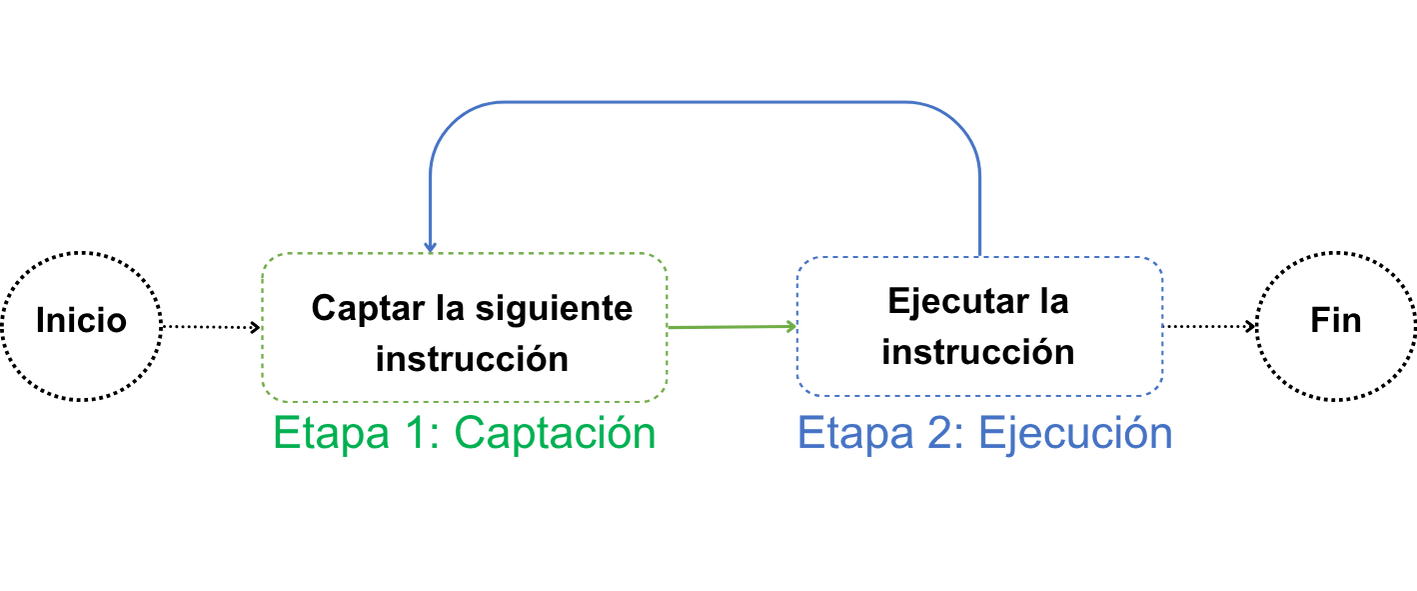
\includegraphics[width=0.85\linewidth]{images/cicloinstruccion3} 

}

\caption{Flujo del ciclo de instrucción en VonSim8}\label{fig:flujoCicloInstruccion}
\end{figure}

\hypertarget{etapa-1-captaciuxf3n}{%
\subsection{Etapa 1: Captación}\label{etapa-1-captaciuxf3n}}

Esta etapa es igual para todas las instrucciones. Su objetivo es leer la instrucción desde la memoria y cargarla en el \textbf{Registro de Instrucciones} (\texttt{IR}). Consta de tres microoperaciones:

\begin{enumerate}
\def\labelenumi{\arabic{enumi}.}
\item
  \textbf{\texttt{MAR} \(\leftarrow\) \texttt{IP}}
  La UC transfiere al \textbf{Registro de Direcciones de Memoria} (\texttt{MAR}) la dirección de la próxima instrucción, almacenada en el \textbf{Puntero de Instrucción} (\texttt{IP}) .
\item
  \textbf{\texttt{MBR} \(\leftarrow\) \texttt{read(Memoria{[}MAR{]})} \textbar{} \texttt{IP} \(\leftarrow\) \texttt{IP} + 1}
  La UC activa la señal de lectura para leer la instrucción ubicada en la dirección contenida en el \texttt{MAR}. El valor leído se guarda en el \textbf{Registro de Datos de Memoria} (\texttt{MBR}) y, al mismo tiempo, el \texttt{IP} se incrementa para apuntar a la siguiente instrucción u operando.
\item
  \textbf{\texttt{IR} \(\leftarrow\) \texttt{MBR}}
  El contenido del \texttt{MBR} se transfiere al \texttt{IR}, dejando la instrucción lista para ser decodificada y ejecutada.
\end{enumerate}

\hypertarget{etapa-2-ejecuciuxf3n}{%
\subsection{Etapa 2: Ejecución}\label{etapa-2-ejecuciuxf3n}}

En esta etapa, el \textbf{decodificador de instrucciones} interpreta el valor en el registro \texttt{IR}. A partir del código de operación, lee las microinstrucciones necesarias en la \textbf{memoria de control} para determinar el tipo de instrucción, la cantidad de operandos y el modo de direccionamiento.

Luego, estas microinstrucciones se envían a \textbf{secuenciador}, que genera las señales de control precisas para ejecutar la operación.

A continuación se detallan las instrucciones más comunes:

\hypertarget{instrucciones-con-dos-operandos-mov-add-sub-y-cmp}{%
\subsubsection{\texorpdfstring{Instrucciones con dos operandos \texttt{MOV}, \texttt{ADD}, \texttt{SUB} y \texttt{CMP}:}{Instrucciones con dos operandos MOV, ADD, SUB y CMP:}}\label{instrucciones-con-dos-operandos-mov-add-sub-y-cmp}}

\begin{itemize}
\tightlist
\item
  \textbf{Destino en registro (\texttt{Rx})}

  \begin{itemize}
  \tightlist
  \item
    \textbf{Modo entre registros (\texttt{Rx}, \texttt{Ry})}

    \begin{enumerate}
    \def\labelenumi{\arabic{enumi}.}
    \setcounter{enumi}{3}
    \tightlist
    \item
      La ejecución se realiza en un solo paso:

      \begin{itemize}
      \tightlist
      \item
        MOV: \textbf{\texttt{Rx} \(\leftarrow\) \texttt{Ry}}
      \item
        ADD: \textbf{\texttt{Rx} \(\leftarrow\) \texttt{Rx} + \texttt{Ry} \textbar{} update(Flags)}
      \item
        SUB: \textbf{\texttt{Rx} \(\leftarrow\) \texttt{Rx} - \texttt{Ry} \textbar{} update(Flags)}
      \item
        CMP: \textbf{\texttt{Rx} - \texttt{Ry} \textbar{} update(Flags)} (solo actualiza flags, no guarda el resultado)
      \end{itemize}
    \end{enumerate}
  \item
    \textbf{Modo directo (\texttt{Rx}, \texttt{{[}Dirección{]}})}

    \begin{enumerate}
    \def\labelenumi{\arabic{enumi}.}
    \setcounter{enumi}{3}
    \tightlist
    \item
      \textbf{\texttt{MAR} \(\leftarrow\) \texttt{IP}} -- Obtener dirección del operando fuente.
    \item
      \textbf{\texttt{MBR} \(\leftarrow\) \texttt{read(Memoria{[}MAR{]})} \textbar{} \texttt{IP} \(\leftarrow\) \texttt{IP} + 1} -- Leer la dirección desde memoria e incrementar IP.
    \item
      \textbf{\texttt{MAR} \(\leftarrow\) \texttt{MBR}} -- Transferir la dirección al MAR.
    \item
      \textbf{\texttt{MBR} \(\leftarrow\) \texttt{read(Memoria{[}MAR{]})}} -- Obtener el dato.
    \item
      Ejecutar la operación:

      \begin{itemize}
      \tightlist
      \item
        MOV: \textbf{\texttt{Rx} \(\leftarrow\) \texttt{MBR}}
      \item
        ADD: \textbf{\texttt{Rx} \(\leftarrow\) \texttt{Rx} + \texttt{MBR} \textbar{} update(Flags)}
      \item
        SUB: \textbf{\texttt{Rx} \(\leftarrow\) \texttt{Rx} - \texttt{MBR} \textbar{} update(Flags)}
      \item
        CMP: \textbf{\texttt{Rx} - \texttt{MBR} \textbar{} update(Flags)}
      \end{itemize}
    \end{enumerate}
  \item
    \textbf{Modo inmediato (\texttt{Rx}, \texttt{Dato})}

    \begin{enumerate}
    \def\labelenumi{\arabic{enumi}.}
    \setcounter{enumi}{3}
    \tightlist
    \item
      \textbf{\texttt{MAR} \(\leftarrow\) \texttt{IP}} -- Obtener dirección del dato inmediato.
    \item
      \textbf{\texttt{MBR} \(\leftarrow\) \texttt{read(Memoria{[}MAR{]})} \textbar{} \texttt{IP} \(\leftarrow\) \texttt{IP} + 1} -- Leer el dato e incrementar IP.
    \item
      Ejecutar la operación (igual que en el caso anterior).
    \end{enumerate}
  \item
    \textbf{Modo indirecto (\texttt{Rx}, \texttt{{[}BL{]}})}

    \begin{enumerate}
    \def\labelenumi{\arabic{enumi}.}
    \setcounter{enumi}{3}
    \tightlist
    \item
      \textbf{\texttt{MAR} \(\leftarrow\) \texttt{BL}} -- Obtener dirección del dato desde el registro BL.
    \item
      \textbf{\texttt{MBR} \(\leftarrow\) \texttt{read(Memoria{[}MAR{]})}} -- Leer el dato.
    \item
      Ejecutar la operación (igual que en el caso anterior).
    \end{enumerate}
  \end{itemize}
\item
  \textbf{Destino en memoria (\texttt{{[}Dirección{]}} o \texttt{{[}BL{]}})}
  En este caso, el resultado de la operación se almacena en una dirección de memoria especificada en la instrucción o indicada por el contenido del registro BL.

  \begin{itemize}
  \tightlist
  \item
    \textbf{Modo Directo (\texttt{{[}Dirección{]}}, \texttt{Ry})}

    \begin{enumerate}
    \def\labelenumi{\arabic{enumi}.}
    \setcounter{enumi}{3}
    \tightlist
    \item
      \textbf{\texttt{MAR} \(\leftarrow\) \texttt{IP}} -- Obtener dirección destino.
    \item
      \textbf{\texttt{MBR} \(\leftarrow\) \texttt{read(Memoria{[}MAR{]})} \textbar{} \texttt{IP} \(\leftarrow\) \texttt{IP} + 1} -- Leer la dirección e incrementar IP.
    \item
      \textbf{\texttt{MAR} \(\leftarrow\) \texttt{MBR}} -- Transferir dirección a MAR.
      Según la instrucción:
    \end{enumerate}

    \begin{itemize}
    \tightlist
    \item
      MOV:

      \begin{enumerate}
      \def\labelenumi{\arabic{enumi}.}
      \setcounter{enumi}{6}
      \tightlist
      \item
        \textbf{\texttt{MBR} \(\leftarrow\) \texttt{Ry}} -- Copiar Ry al MBR.
      \item
        \textbf{\texttt{write(Memoria{[}MAR{]})} \(\leftarrow\) \texttt{MBR}} -- Escribir en memoria.
      \end{enumerate}
    \item
      ADD, SUB, CMP:

      \begin{enumerate}
      \def\labelenumi{\arabic{enumi}.}
      \setcounter{enumi}{6}
      \tightlist
      \item
        \textbf{\texttt{MBR} \(\leftarrow\) \texttt{read(Memoria{[}MAR{]})}} -- Leer el dato.
      \item
        Ejecutar la operación:

        \begin{itemize}
        \tightlist
        \item
          ADD: \textbf{\texttt{MBR} \(\leftarrow\) \texttt{MBR} + \texttt{Ry} \textbar{} update(Flags)}
        \item
          SUB: \textbf{\texttt{MBR} \(\leftarrow\) \texttt{MBR} - \texttt{Ry} \textbar{} update(Flags)}
        \item
          CMP: \textbf{\texttt{MBR} - \texttt{Ry} \textbar{} update(Flags)}
        \end{itemize}
      \item
        Si es \texttt{ADD} o \texttt{SUB}: \textbf{\texttt{write(Memoria{[}MAR{]})} \(\leftarrow\) \texttt{MBR}} -- Escribir en memoria.
      \end{enumerate}
    \end{itemize}
  \item
    \textbf{Modo Indirecto (\texttt{{[}BL{]}}, \texttt{Ry})}

    \begin{enumerate}
    \def\labelenumi{\arabic{enumi}.}
    \setcounter{enumi}{3}
    \tightlist
    \item
      \textbf{\texttt{MAR} \(\leftarrow\) \texttt{BL}} -- Transferir dirección de destino (en BL) a MAR.
      Según la instrucción:
    \end{enumerate}

    \begin{itemize}
    \tightlist
    \item
      MOV:

      \begin{enumerate}
      \def\labelenumi{\arabic{enumi}.}
      \setcounter{enumi}{4}
      \tightlist
      \item
        \textbf{\texttt{MBR} \(\leftarrow\) \texttt{Ry}} -- Copiar Ry al MBR.
      \item
        \textbf{\texttt{write(Memoria{[}MAR{]})} \(\leftarrow\) \texttt{MBR}} -- Escribir en memoria.
      \end{enumerate}
    \item
      ADD, SUB, CMP:

      \begin{enumerate}
      \def\labelenumi{\arabic{enumi}.}
      \setcounter{enumi}{4}
      \tightlist
      \item
        \textbf{\texttt{MBR} \(\leftarrow\) \texttt{read(Memoria{[}MAR{]})}} -- Leer el dato.
      \item
        Ejecutar la operación (igual que en el caso anterior).
      \item
        Si es \texttt{ADD} o \texttt{SUB}: \textbf{\texttt{write(Memoria{[}MAR{]})} \(\leftarrow\) \texttt{MBR}} -- Escribir en memoria.
      \end{enumerate}
    \end{itemize}
  \item
    \textbf{Modo Directo-Inmediato (\texttt{{[}Dirección{]}}, \texttt{Dato})}

    \begin{enumerate}
    \def\labelenumi{\arabic{enumi}.}
    \setcounter{enumi}{3}
    \tightlist
    \item
      \textbf{\texttt{MAR} \(\leftarrow\) \texttt{IP}} -- Obtener dirección destino.
    \item
      \textbf{\texttt{MBR} \(\leftarrow\) \texttt{read(Memoria{[}MAR{]})} \textbar{} \texttt{IP} \(\leftarrow\) \texttt{IP} + 1} -- Leer dirección e incrementar IP.
    \item
      \textbf{\texttt{MAR} \(\leftarrow\) \texttt{IP} \textbar{} \texttt{ri} \(\leftarrow\) \texttt{MBR}} -- Preparar para leer el dato y guardar la dirección destino en un registro intermedio (ri).
    \item
      \textbf{\texttt{MBR} \(\leftarrow\) \texttt{read(Memoria{[}MAR{]})} \textbar{} \texttt{IP} \(\leftarrow\) \texttt{IP} + 1} -- Leer dato e incrementar IP.
      Según la instrucción:
    \end{enumerate}

    \begin{itemize}
    \tightlist
    \item
      MOV:

      \begin{enumerate}
      \def\labelenumi{\arabic{enumi}.}
      \setcounter{enumi}{7}
      \tightlist
      \item
        \textbf{\texttt{MAR} \(\leftarrow\) \texttt{ri}} -- Copiar dirección destino.
      \item
        \textbf{\texttt{write(Memoria{[}MAR{]})} \(\leftarrow\) \texttt{MBR}} -- Escribir en memoria.
      \end{enumerate}
    \item
      ADD, SUB, CMP:

      \begin{enumerate}
      \def\labelenumi{\arabic{enumi}.}
      \setcounter{enumi}{7}
      \tightlist
      \item
        \textbf{\texttt{MAR} \(\leftarrow\) \texttt{ri} \textbar{} \texttt{id} \(\leftarrow\) \texttt{MBR}} -- Cargar dirección destino y guardar el valor inmediato en id.
      \item
        \textbf{\texttt{MBR} \(\leftarrow\) \texttt{read(Memoria{[}MAR{]})}} -- Leer el valor actual de destino.
      \item
        Ejecutar la operación:

        \begin{itemize}
        \tightlist
        \item
          ADD: \textbf{\texttt{MBR} \(\leftarrow\) \texttt{MBR} + \texttt{id} \textbar{} update(Flags)}
        \item
          SUB: \textbf{\texttt{MBR} \(\leftarrow\) \texttt{MBR} - \texttt{id} \textbar{} update(Flags)}
        \item
          CMP: \textbf{\texttt{MBR} - \texttt{id} \textbar{} update(Flags)}
        \end{itemize}
      \item
        Si es \texttt{ADD} o \texttt{SUB}: \textbf{\texttt{write(Memoria{[}MAR{]})} \(\leftarrow\) \texttt{MBR}} -- Escribir en memoria.
      \end{enumerate}
    \end{itemize}
  \item
    \textbf{Modo Indirecto-Inmediato (\texttt{{[}BL{]}}, \texttt{Dato})}

    \begin{enumerate}
    \def\labelenumi{\arabic{enumi}.}
    \setcounter{enumi}{3}
    \tightlist
    \item
      \textbf{\texttt{MAR} \(\leftarrow\) \texttt{IP}} -- Obtener dirección del dato inmediato.
    \item
      \textbf{\texttt{MBR} \(\leftarrow\) \texttt{read(Memoria{[}MAR{]})} \textbar{} \texttt{IP} \(\leftarrow\) \texttt{IP} + 1} -- Leer dato e incrementar IP.
      Según la instrucción:
    \end{enumerate}

    \begin{itemize}
    \tightlist
    \item
      MOV:

      \begin{enumerate}
      \def\labelenumi{\arabic{enumi}.}
      \setcounter{enumi}{5}
      \tightlist
      \item
        \textbf{\texttt{MAR} \(\leftarrow\) \texttt{BL}} -- Copiar dirección de destino.
      \item
        \textbf{\texttt{write(Memoria{[}MAR{]})} \(\leftarrow\) \texttt{MBR}}
      \end{enumerate}
    \item
      ADD, SUB, CMP:

      \begin{enumerate}
      \def\labelenumi{\arabic{enumi}.}
      \setcounter{enumi}{5}
      \tightlist
      \item
        \textbf{\texttt{MAR} \(\leftarrow\) \texttt{BL} \textbar{} \texttt{id} \(\leftarrow\) \texttt{MBR}} -- Cargar la dirección destino y guardar el valor inmediato en id.
      \item
        \textbf{\texttt{MBR} \(\leftarrow\) \texttt{read(Memoria{[}MAR{]})}} -- Leer el valor actual de destino.
      \item
        Ejecutar la operación (igual que en el caso anterior).
      \item
        Si es \texttt{ADD} o \texttt{SUB}: \textbf{\texttt{write(Memoria{[}MAR{]})} \(\leftarrow\) \texttt{MBR}} -- Escribir en memoria.
      \end{enumerate}
    \end{itemize}
  \end{itemize}
\end{itemize}

\hypertarget{instrucciones-con-un-operando-jmp-y-jxx}{%
\subsubsection{\texorpdfstring{Instrucciones con un operando \texttt{JMP} y \texttt{Jxx}:}{Instrucciones con un operando JMP y Jxx:}}\label{instrucciones-con-un-operando-jmp-y-jxx}}

\begin{itemize}
\tightlist
\item
  \textbf{Salto a (\texttt{Dirección})}
  Tanto incondicional \texttt{JMP} como condicionales \texttt{Jxx} tienen estos pasos:

  \begin{enumerate}
  \def\labelenumi{\arabic{enumi}.}
  \setcounter{enumi}{3}
  \tightlist
  \item
    \textbf{\texttt{MAR} \(\leftarrow\) \texttt{IP}} -- Obtener la dirección del salto.
  \item
    \textbf{\texttt{MBR} \(\leftarrow\) \texttt{read(Memoria{[}MAR{]})}; \texttt{IP} \(\leftarrow\) \texttt{IP} + 1} -- Leer la dirección de destino e incrementar IP.
  \end{enumerate}

  Según la instrucción:

  \begin{itemize}
  \tightlist
  \item
    JMP:

    \begin{enumerate}
    \def\labelenumi{\arabic{enumi}.}
    \setcounter{enumi}{5}
    \tightlist
    \item
      \textbf{\texttt{IP} \(\leftarrow\) \texttt{MBR}}
    \end{enumerate}
  \item
    Jxx:

    \begin{enumerate}
    \def\labelenumi{\arabic{enumi}.}
    \setcounter{enumi}{5}
    \tightlist
    \item
      \textbf{\texttt{IP} \(\leftarrow\) \texttt{MBR}} si se cumple la condición del flag \texttt{xx}; en caso contrario, continúa con la siguiente instrucción.
    \end{enumerate}
  \end{itemize}
\end{itemize}

\hypertarget{instrucciones-sin-operandos}{%
\subsubsection{Instrucciones sin operandos}\label{instrucciones-sin-operandos}}

\begin{itemize}
\tightlist
\item
  HLT:

  \begin{enumerate}
  \def\labelenumi{\arabic{enumi}.}
  \setcounter{enumi}{3}
  \tightlist
  \item
    Detiene la ejecución de la CPU.
  \end{enumerate}
\end{itemize}

\hypertarget{muxf3dulo-de-entradasalida-e-interrupciones}{%
\section{Módulo de Entrada/Salida e interrupciones}\label{muxf3dulo-de-entradasalida-e-interrupciones}}

El simulador permite configurar la conexión de diversos módulos de entrada/salida y otros dispositivos al bus principal, agrupados en las siguientes categorías:
- Teclado y pantalla.
- Un módulo PIO, que puede conectarse a LEDs e interruptores.
- Módulo Handshake, con posibilidad de conexión a una impresora, con o sin controlador PIC.
- Un controlador PIC, que interactúa con la tecla F10 para generar interrupciones, junto con un temporizador y su reloj asociado.

La Figura \ref{fig:dispositivos} muestra una visión general de los dispositivos que pueden conectarse al simulador.

\begin{figure}

{\centering 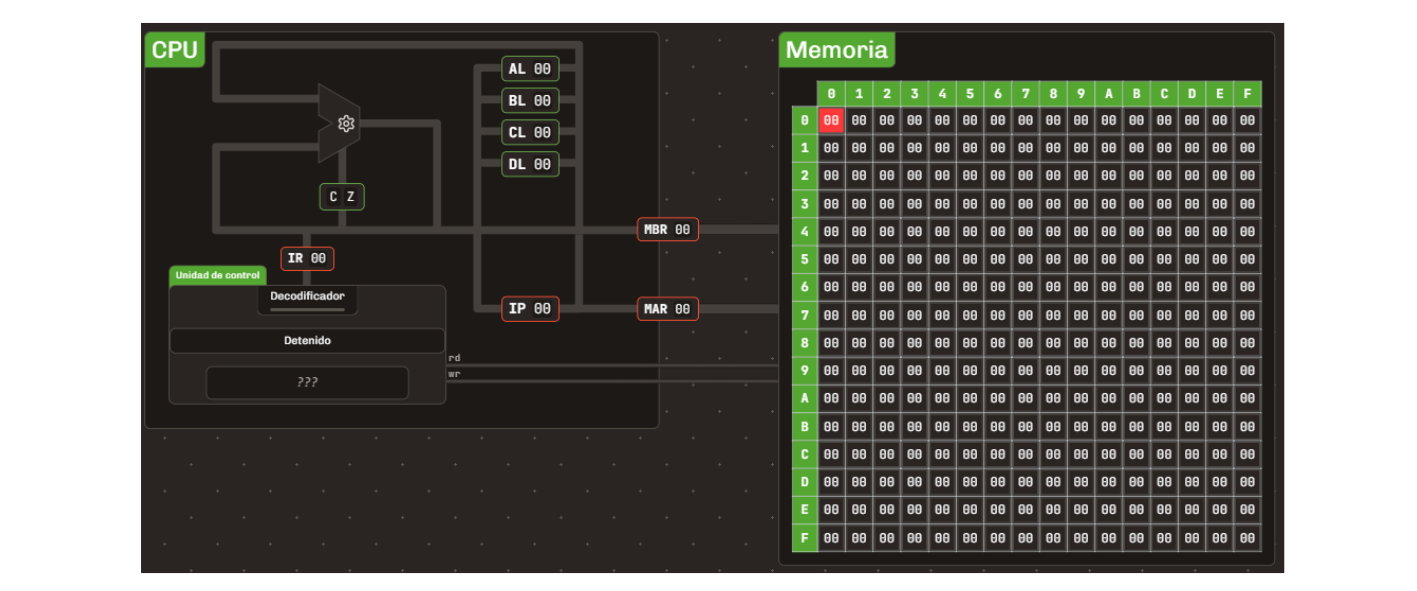
\includegraphics[width=0.85\linewidth]{images/esquemavonsim8} 

}

\caption{Arquitectura general del simulador}\label{fig:dispositivos}
\end{figure}

El componente chipSelect se encarga de activar el dispositivo correspondiente en cada momento. Para ello, recibe las señales de control del CPU junto con el bus de direcciones, y genera las señales de selección de chip (CS) necesarias para habilitar el dispositivo adecuado.

Para interactuar con los módulos de entrada y salida, es necesario incorporar nuevas instrucciones al repertorio del procesador. Estas instrucciones permiten la comunicación con los puertos de E/S y la gestión de interrupciones. La Tabla \ref{tab:tisa} detalla las categorías de instrucciones, sus códigos de operación y las acciones que realizan.

\begin{table}[!h]
\centering
\caption{\label{tab:tisa}Categoría de instrucciones y códigos de operación en VonSim8}
\centering
\resizebox{\ifdim\width>\linewidth\linewidth\else\width\fi}{!}{
\fontsize{10}{12}\selectfont
\begin{tabular}[t]{>{\centering\arraybackslash}p{4cm}|>{\centering\arraybackslash}p{4cm}>{\centering\arraybackslash}p{3cm}>{\raggedright\arraybackslash}p{8cm}}
\toprule
\multicolumn{1}{>{\centering\arraybackslash}p{4cm}}{\cellcolor[HTML]{D3D3D3}{\textbf{Categoría}}} & \multicolumn{1}{>{\centering\arraybackslash}p{4cm}}{\cellcolor[HTML]{D3D3D3}{\textbf{Instrucción}}} & \multicolumn{1}{>{\centering\arraybackslash}p{3cm}}{\cellcolor[HTML]{D3D3D3}{\textbf{Código operación}}} & \multicolumn{1}{>{\centering\arraybackslash}p{8cm}}{\cellcolor[HTML]{D3D3D3}{\textbf{Acción}}}\\
\midrule
\textbf{Transferencia de datos} & MOV & {0, 1, 2} & Copiar entre registros, cargar a registro, almacenar en memoria\\
\addlinespace[10pt]
\textbf{Procesamiento de datos} & ADD & {3, 4, 5} & Operación aritmética: operando1 ← operando1 + operando2\\
\addlinespace[10pt]
\textbf{} & SUB & {6, 7, 8} & Operación aritmética: operando1 ← operando1 - operando2\\
\addlinespace[10pt]
\textbf{} & CMP & {9, 10, 11} & Comparación: operando1 - operando2 (no actualiza el destino)\\
\addlinespace[10pt]
\textbf{Control de flujo} & JMP / Jxx / CALL / INT & {12} & Salto incondicional JMP, condicionales Jxx, subrutina CALL, llamar rutina de interrupción INT\\
\addlinespace[10pt]
\addlinespace
\textbf{Gestión de flujo} & RET / IRET / CLI / STI / HLT & {13} & Retorno subrutina RET, retornar de interrupción IRET,  deshabilita interrupciones CLI, habilita interrupciones STI, detener CPU HLT\\
\addlinespace[10pt]
\textbf{Manejo de pila y E/S} & PUSH / POP / OUT / IN & {14} & Poner en la pila PUSH, retirar de la pila POP, enviar a puerto OUT, recibir desde puerto IN\\
\addlinespace[10pt]
\textbf{Miscelánea} & AND / OR / XOR / NOT / NEG / INC / DEC & {15} & Operaciones lógicas y aritméticas\\
\addlinespace[10pt]
\bottomrule
\end{tabular}}
\end{table}

El simulador utiliza un código de operación de 4 bits para las instrucciones, lo que simplifica la arquitectura del sistema pero limita el número máximo de instrucciones implementables a 16 opciones diferentes. Con el objetivo de ampliar el repertorio de instrucciones sin incrementar el tamaño de la codificación, se adoptó una estrategia de agrupación para el código de operación 15.

Bajo esta implementación, las instrucciones lógicas (AND, OR y XOR) comparten el código de operación 15 con las instrucciones aritméticas de un operando (INC, DEC, NEG y NOT). Esta decisión de diseño permite mantener la compatibilidad con los modos de direccionamiento establecidos para las instrucciones aritméticas de dos operandos (ADD, SUB y CMP), garantizando consistencia en la interfaz del simulador mientras se maximiza la funcionalidad dentro de las limitaciones impuestas por el esquema de codificación de 4 bits.

Esta solución representa un compromiso eficaz entre la simplicidad arquitectural y la capacidad funcional del simulador, permitiendo una mayor diversidad de operaciones sin comprometer la claridad pedagógica del diseño.

\hypertarget{pila-y-subrutinas}{%
\subsection{Pila y subrutinas}\label{pila-y-subrutinas}}

El procesador implementa una pila como método de almacenamiento, accesible tanto por el usuario como por la CPU para su funcionamiento interno. La pila opera bajo el esquema \emph{Last In, First Out} (LIFO), es decir, el último elemento en ingresar es el primero en salir. Está ubicada en la memoria principal, comenzando en la dirección más alta (\texttt{FFh}) y creciendo hacia direcciones más bajas (\texttt{FEh}, \texttt{FCh}, etc.). El tope de la pila se gestiona mediante el registro \texttt{SP}, y cada elemento almacenado ocupa 8 bits.

Además, el procesador permite el uso de subrutinas, que son fragmentos de código reutilizables y pueden ser invocados desde cualquier parte del programa. Para llamar a una subrutina se utiliza la instrucción {[}\texttt{CALL}{]}, que apila el valor actual de \texttt{IP} y salta a la dirección de la subrutina, modificando el \texttt{IP} para apuntar a la primera instrucción de la misma. El retorno se realiza mediante la instrucción {[}\texttt{RET}{]}, que desapila la dirección previamente guardada y restaura el \texttt{IP}, permitiendo continuar la ejecución justo después de la llamada.

Ejemplo de subrutina:

\begin{lstlisting}
      mov al, 1
      mov bl, 2
      mov cl, 3
      call sum3
      ; ax = 6
      hlt

      ; suma al, bl y cl
      sum3: add al, bl
            add al, cl
            ret\end{lstlisting}

\hypertarget{interrupciones-y-llamadas-al-sistema}{%
\subsection{Interrupciones y llamadas al sistema}\label{interrupciones-y-llamadas-al-sistema}}

El simulador VonSim8 incorpora un teclado y una pantalla como dispositivos de entrada y salida, permitiendo la interacción básica entre el usuario y el sistema para la entrada de datos y la visualización de resultados.

\begin{figure}

{\centering 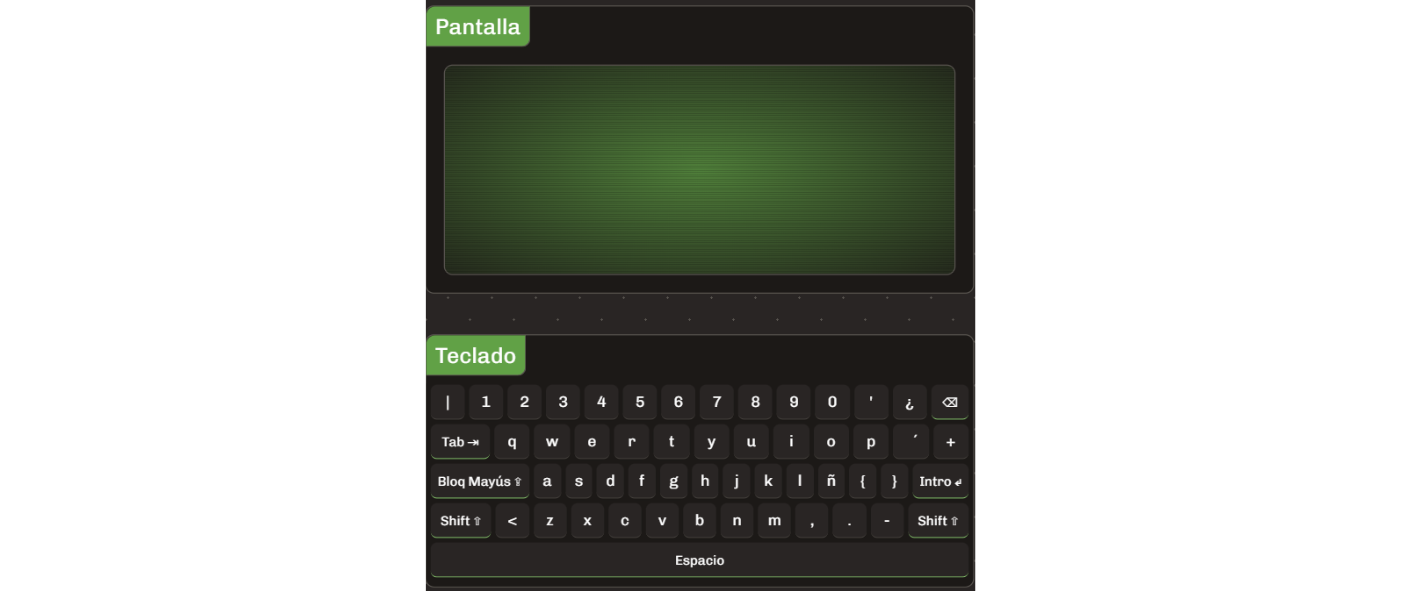
\includegraphics[width=0.85\linewidth]{images/tecladopantalla} 

}

\caption{Teclado y pantalla}\label{fig:tecladopantalla}
\end{figure}

El vector de interrupciones está predefinido en posiciones reservadas de la memoria principal, donde se almacenan las direcciones de las rutinas del sistema para interactuar con el teclado y la pantalla. En el caso de las interrupciones por software, el número de interrupción se indica como operando en la instrucción \texttt{INT}. Al producirse una interrupción, el procesador ejecuta la rutina asociada al número de interrupción, cuya dirección de inicio se obtiene del vector de interrupciones. Este vector ocupa las celdas de memoria desde \texttt{00h} hasta \texttt{07h}, y cada elemento tiene 1 byte de longitud, correspondiendo cada uno a la dirección de inicio de la rutina respectiva.

El procesador admite interrupciones tanto por hardware como por software, generadas por el PIC o por la instrucción \texttt{INT}, respectivamente. Para que las interrupciones por hardware sean atendidas, el procesador debe tener habilitada la bandera de interrupciones (I=1). En ambos casos, se debe proporcionar un número de interrupción entre \texttt{0} y \texttt{7}.

El procedimiento que sigue el procesador ante una interrupción es el siguiente:

\begin{enumerate}
\def\labelenumi{\arabic{enumi}.}
\tightlist
\item
  obtiene el número de la interrupción (0-7),
\item
  apila el registro \texttt{Flags},
\item
  inhabilita las interrupciones \texttt{I=0},
\item
  apila el registro \texttt{IP},
\item
  obtiene la dirección de la rutina de interrupción desde el vector de interrupciones,
\item
  carga en el \texttt{IP} la dirección de la rutina de interrupción.
\end{enumerate}

La rutina de interrupción se ejecuta como una subrutina, pero finaliza con la instrucción \texttt{IRET} en lugar de \texttt{RET}.

\hypertarget{llamadas-al-sistema}{%
\subsection{Llamadas al sistema}\label{llamadas-al-sistema}}

El simulador permite realizar llamadas al sistema (syscalls) mediante interrupciones, utilizando el número de interrupción correspondiente. Los números de interrupción reservados para llamadas al sistema son:

\begin{itemize}
\tightlist
\item
  \texttt{INT\ 0}: termina la ejecución del programa (equivalente a \texttt{HLT});
\item
  \texttt{INT\ 6}: lee un carácter del teclado;
\item
  \texttt{INT\ 7}: escribe una cadena de caracteres en pantalla.
\end{itemize}

Las direcciones del vector de interrupciones asociadas a estas llamadas están protegidas por el sistema y no pueden ser modificadas por el usuario. El contenido de las rutinas correspondientes se encuentra almacenado en el monitor del sistema en las direcciones \texttt{A0h}, \texttt{B0h} y \texttt{C0h}, respectivamente.

\hypertarget{pantalla}{%
\subsection{Pantalla}\label{pantalla}}

La pantalla es un dispositivo de salida que permite mostrar caracteres. La forma de comunicarse con la pantalla es mediante una llamada al sistema. Esto es así por simplicidad, ya que una pantalla real es mucho más compleja.

Con la llamada INT 7 se escribe una cadena de caracteres en la pantalla. Recibe dos parámetros:

AL: longitud de la cadena a imprimir
BL: dirección de memoria donde empieza la cadena

Ejemplo de hola mundo en lenguaje ensamblador para el simulador VonSim8:

\begin{lstlisting}
cadena DB `Hola!`
MOV BL, offset cadena
MOV AL, 5
INT 7
; Se imprime Hola! (sin las comillas) en la pantalla.
HLT\end{lstlisting}

Hay tres caracteres especiales:

\begin{itemize}
\tightlist
\item
  el carácter de retroceso (\texttt{BS}, 8 en decimal) borra el carácter previo;
\item
  el carácter de salto de línea (\texttt{LF}, 10 en decimal) imprime, en efecto, un salto de línea --- útil para no imprimir todo en una sola línea;
\item
  el carácter de \emph{form feed} (\texttt{FF}, 12 en decimal) limpia la pantalla.
\end{itemize}

\hypertarget{teclado}{%
\subsection{Teclado}\label{teclado}}

El teclado se modela como un vector de 16 posiciones, cada una capaz de almacenar un carácter ASCII. La pantalla, por su parte, se representa como una matriz de 16×16 que permite visualizar caracteres, facilitando así la comprensión del manejo de entrada y salida de datos en una arquitectura computacional simplificada.

El teclado es un dispositivo de entrada que permite al usuario ingresar caracteres al sistema. La forma de comunicarse con el teclado es mediante una llamada al sistema. Esto es así por simplicidad, ya que un teclado real es mucho más complejo.

Con la llamada INT 6 se detiene la ejecución del código hasta que se presione una tecla en el teclado. El carácter que correspona será guardado en la dirección de memoria almacenada en BL según su representación en ASCII.

\begin{lstlisting}
car db 0
mov bl, offset car
int 6
hlt

; El carácter escrito se almacenó en 'car'.
; Por ejemplo, si el usuario presionó la tecla 'a', entonces
; se almacena el valor 61h en 'car'.\end{lstlisting}

\hypertarget{puertos-de-es}{%
\subsection{Puertos de E/S}\label{puertos-de-es}}

La memoria de entrada/salida está completamente separada de la memoria principal. Para interactuar con ella, se emplean exclusivamente las instrucciones {[}IN{]} y {[}OUT{]}. Cuando se requiere acceder a un módulo de entrada/salida, la {[}CPU{]} activa la señal IO/M, lo que provoca que un selector de chips (chip select) interprete la dirección presente en el bus de direcciones y envíe la señal de activación al módulo correspondiente.

El rango de direcciones asignado a la memoria de entrada/salida abarca desde \texttt{00h} hasta \texttt{FFh}, lo que permite un total de 256 direcciones. A continuación, se presentan las direcciones de entrada/salida disponibles en el simulador, todas de 8 bits:

\begin{table}[!h]
\centering
\caption{\label{tab:tpuertos}Módulos, direcciones y nombres del simulador}
\centering
\resizebox{\ifdim\width>\linewidth\linewidth\else\width\fi}{!}{
\fontsize{10}{12}\selectfont
\begin{tabular}[t]{>{\centering\arraybackslash}p{3cm}|>{\centering\arraybackslash}p{2cm}>{\centering\arraybackslash}p{3cm}}
\toprule
\multicolumn{1}{>{\centering\arraybackslash}p{3cm}}{\cellcolor[HTML]{D3D3D3}{\textbf{Módulo}}} & \multicolumn{1}{>{\centering\arraybackslash}p{2cm}}{\cellcolor[HTML]{D3D3D3}{\textbf{Dirección}}} & \multicolumn{1}{>{\centering\arraybackslash}p{3cm}}{\cellcolor[HTML]{D3D3D3}{\textbf{Nombre}}}\\
\midrule
\cellcolor[HTML]{F0F0F0}{\textbf{Timer}} & \cellcolor[HTML]{F0F0F0}{10h} & \cellcolor[HTML]{F0F0F0}{CONT}\\
\textbf{} & 11h & COMP\\
\addlinespace[5pt]
\cellcolor[HTML]{F0F0F0}{\textbf{PIC}} & \cellcolor[HTML]{F0F0F0}{20h} & \cellcolor[HTML]{F0F0F0}{EOI}\\
\textbf{} & 21h & IMR\\
\textbf{} & 22h & IRR\\
\addlinespace
\textbf{} & 23h & ISR\\
\textbf{} & 24h & INT0\\
\textbf{} & 25h & INT1\\
\textbf{} & 26h & INT2\\
\textbf{} & 27h & INT3\\
\addlinespace
\cellcolor[HTML]{F0F0F0}{\textbf{PIO}} & \cellcolor[HTML]{F0F0F0}{28h} & \cellcolor[HTML]{F0F0F0}{PA}\\
\textbf{} & 29h & PB\\
\textbf{} & 2Ah & CA\\
\textbf{} & 2Bh & CB\\
\addlinespace[5pt]
\cellcolor[HTML]{F0F0F0}{\textbf{Handshake}} & \cellcolor[HTML]{F0F0F0}{40h} & \cellcolor[HTML]{F0F0F0}{DATA}\\
\addlinespace
\textbf{} & 41h & STATE\\
\bottomrule
\end{tabular}}
\end{table}

\hypertarget{instrucciones-in-y-out}{%
\subsection{Instrucciones IN y OUT}\label{instrucciones-in-y-out}}

La comunicación con los módulos de entrada/salida se realiza a través de puertos, que son direcciones específicas dentro del espacio de direcciones del procesador. En este simulador, se implementan dos instrucciones fundamentales para gestionar esta comunicación:

\begin{itemize}
\tightlist
\item
  \texttt{OUT\ puerto,\ AL}: envía el contenido del registro \texttt{AL} al puerto especificado. El puerto es una dirección de 8 bits, lo que permite un total de 256 puertos diferentes (de \texttt{00h} a \texttt{FFh}). Esta instrucción se utiliza para transmitir datos a dispositivos externos, como impresoras o pantallas.
\item
  \texttt{IN\ AL,\ puerto}: recibe un byte desde el puerto especificado y lo almacena en el registro \texttt{AL}. Al igual que la instrucción \texttt{OUT}, el puerto es una dirección de 8 bits.
\end{itemize}

\hypertarget{muxf3dulo-pio}{%
\subsection{Módulo PIO}\label{muxf3dulo-pio}}

El módulo de entrada/salida programada (Programmed Input-Output, PIO) actúa como interfaz entre la CPU y los dispositivos periféricos genéricos. Su diseño está basado en el controlador PPI 8255 de Intel, específicamente en su modo \texttt{0}, pero incorpora modificaciones orientadas a simplificar su funcionamiento para fines educativos \protect\hyperlink{ref-intel8086manual}{{[}51{]}}.

El módulo cuenta con dos puertos bidireccionales de 8 bits (A y B) que pueden ser configurados de manera independiente. Su arquitectura incluye cuatro registros accesibles:

\begin{itemize}
\tightlist
\item
  PA (dirección 30h en el espacio de memoria E/S): registro de datos del puerto A
\item
  PB (dirección 31h en el espacio de memoria E/S): registro de datos del puerto B
\item
  CA (dirección 32h en el espacio de memoria E/S): registro de configuración del puerto A
\item
  CB (dirección 33h en el espacio de memoria E/S): registro de configuración del puerto B
\end{itemize}

La configuración de cada puerto se define a través de sus respectivos registros de control (CA y CB). Cada bit del registro de configuración determina la dirección del bit correspondiente en el puerto de datos: un valor \texttt{0} configura el bit como salida, mientras que un valor \texttt{1} lo configura como entrada. Por ejemplo, si CA = 00001111b, los cuatro bits más significativos del puerto A funcionarán como salidas, y los cuatro bits menos significativos como entradas. El puerto B opera de manera idéntica mediante su registro CB.

Este módulo PIO puede conectarse a diferentes tipos de dispositivos periféricos, como LEDs y interruptores, o a dispositivos más complejos como una impresora, proporcionando así una interfaz versátil para la comunicación con el mundo exterior.

\hypertarget{leds}{%
\subsubsection{Leds}\label{leds}}

Los diodos emisores de luz (LEDs) funcionan como dispositivos de salida y están conectados al puerto B del módulo PIO. Su control se realiza mediante la manipulación del registro de datos PB (dirección 31h) en conjunto con el registro de configuración CB (dirección 33h).

Para que los LEDs respondan correctamente, es necesario configurar previamente el puerto B como salida escribiendo el valor apropiado en el registro CB. Una vez configurado correctamente el PIO, cualquier modificación en el valor del registro PB se reflejará inmediatamente en el estado de los LEDs correspondientes. En caso de que la configuración del puerto sea incorrecta o se omita este paso, los LEDs permanecerán apagados independientemente de los valores escritos en PB.

Esta configuración permite controlar individualmente cada LED mediante los bits del puerto, ofreciendo flexibilidad para crear patrones luminosos o indicadores visuales en aplicaciones educativas y de demostración.

Las luces o LEDs están conectadas al puerto PB/CB del PIO y funcionan como dispositivos de salida. Su estado solo puede modificarse alterando el valor del puerto PB. Estos cambios se reflejarán en las luces si el PIO está configurado correctamente; de lo contrario, las luces permanecerán apagadas.

\begin{lstlisting}
; Enciende las luces (una sí, una no): 1010 1010b
; 31h = PB --> puerto de datos para las luces (LEDs)
; 33h = CB --> puerto de control para las luces

; Configura todos los bits de PB como salida para controlar las luces
mov al, 0                ; 0000 0000b: todos los bits de PB en modo salida
out 33h, al              ; Escribe en CB para configurar PB como salida

; Enciende las luces alternadas: 1010 1010b (170 decimal)
mov al, 170              ; 1010 1010b: enciende LEDs pares, apaga impares
out 31h, al              ; Escribe el valor en PB para actualizar las luces

hlt                      ; Detiene la ejecución del programa\end{lstlisting}

\hypertarget{interruptores}{%
\subsubsection{interruptores}\label{interruptores}}

Los interruptores (también denominados llaves) funcionan como dispositivos de entrada conectados al puerto A del módulo PIO. Su operación se gestiona mediante el registro de datos PA (dirección 30h) y el registro de configuración CA (dirección 32h).

Para que los interruptores operen correctamente, es fundamental configurar previamente el puerto A como entrada mediante el registro CA. Una vez establecida la configuración apropiada, cualquier cambio en el estado físico de los interruptores se reflejará automáticamente en los bits correspondientes del registro PA, permitiendo al programa leer su estado actual.

Es importante destacar que la comunicación es unidireccional desde los dispositivos hacia el procesador: aunque es posible escribir valores directamente en el registro PA mediante software, estos cambios no alterarán el estado físico de los interruptores. Los dispositivos de entrada mantienen su estado independientemente de las modificaciones realizadas por programa en sus registros asociados, garantizando así la integridad de la información proveniente del mundo exterior.

\begin{lstlisting}
; Leer el valor de las llaves como una contraseña hasta que el usuario la adivine

clave db 15               ; Contraseña esperada: 00001111 (en decimal 15)
mensaje_ok db 'Bienvenido!' ; Mensaje a mostrar si la contraseña es correcta

; Configurar PA (Puerto A) como entrada
mov al, 15                ; 00001111b: configura los primeros 4 bits de PA como entrada
out 32h, al               ; Escribe en CA para configurar PA

bucle:
    in al, 30h            ; Lee el valor actual de las llaves desde PA
    cmp al, clave         ; Compara el valor leído con la contraseña
    jz Mostrar_Mensaje    ; Si coincide, salta a Mostrar_Mensaje
    jmp bucle             ; Si no coincide, vuelve a intentar

Mostrar_Mensaje:
    mov bl, offset mensaje_ok ; BL apunta al mensaje de éxito
    mov al, 11                ; Longitud del mensaje (Bienvenido! tiene 11 caracteres)
    int 7
    hlt                       ; Detiene la ejecución del programa\end{lstlisting}

\hypertarget{muxf3dulo-handshake}{%
\subsection{Módulo Handshake}\label{muxf3dulo-handshake}}

El módulo Handshake es un controlador especializado diseñado para facilitar la comunicación con impresoras que utilizan el protocolo Centronics. Su diseño se inspira en el controlador PPI 8255 de Intel, operando en modo ``1'', pero incluye modificaciones específicas para simplificar su uso y comprensión en entornos educativos.

El módulo cuenta con una arquitectura simplificada basada en dos registros de 8 bits:

\begin{itemize}
\tightlist
\item
  \textbf{Registro de datos}: ubicado en la dirección 40h del espacio de memoria de E/S.
\item
  \textbf{Registro de estado}: ubicado en la dirección 41h del espacio de memoria de E/S.
\end{itemize}

La estructura de estos registros se organiza de la siguiente manera:

\begin{verbatim}
Datos  = DDDD DDDD
Estado = I___ __SB
\end{verbatim}

\hypertarget{funcionamiento-del-registro-de-datos}{%
\subsubsection{Funcionamiento del registro de datos}\label{funcionamiento-del-registro-de-datos}}

El registro de datos almacena el carácter que se desea imprimir, codificado en formato ASCII. Una característica destacada del módulo Handshake es su capacidad de automatización: cada vez que la CPU escribe un valor en este registro, el controlador genera automáticamente un flanco ascendente en la señal strobe, iniciando el proceso de impresión sin necesidad de intervención adicional por parte del software.

\hypertarget{funcionamiento-del-registro-de-estado}{%
\subsubsection{Funcionamiento del registro de estado}\label{funcionamiento-del-registro-de-estado}}

El registro de estado gestiona las señales de control y supervisión del protocolo de comunicación. Sus principales componentes son:

\begin{itemize}
\tightlist
\item
  \textbf{Bits S y B (strobe y busy)}: los dos bits menos significativos controlan las señales de comunicación, con diferencias clave respecto a la implementación en el PIO:

  \begin{itemize}
  \tightlist
  \item
    El bit busy es de solo lectura y refleja automáticamente el estado de la impresora
  \item
    El bit strobe permanece normalmente en 0 y es gestionado automáticamente por el módulo. Cuando la CPU escribe un 1 en el bit strobe, se genera un flanco ascendente que transmite los datos almacenados en el registro de datos, retornando automáticamente a 0.
  \end{itemize}
\item
  \textbf{Bit I (interrupción)}: El bit más significativo controla el sistema de interrupciones del módulo. Cuando este bit está habilitado (I=1) y la impresora se encuentra disponible (B=0), el módulo Handshake genera una interrupción por hardware a través de la línea INT2 del controlador PIC, notificando al sistema que la impresora está lista para recibir nuevos datos.
\end{itemize}

Esta implementación ofrece una interfaz intuitiva para el control de impresoras, automatizando aspectos críticos del protocolo de comunicación y manteniendo la flexibilidad necesaria para comprender los fundamentos de la interacción con dispositivos periféricos.

\hypertarget{ejemplo-de-uso-del-muxf3dulo-handshake-con-sondeo}{%
\subsubsection{Ejemplo de uso del módulo Handshake con sondeo}\label{ejemplo-de-uso-del-muxf3dulo-handshake-con-sondeo}}

Para imprimir utilizando el módulo Handshake, se deben seguir los siguientes pasos:

\begin{enumerate}
\def\labelenumi{\arabic{enumi}.}
\tightlist
\item
  Verificar que el buffer no esté lleno (flag busy).
\item
  Escribir el carácter en el registro de datos.
\end{enumerate}

Además de los caracteres ASCII comunes, el módulo admite caracteres especiales útiles para la impresión:
- Salto de línea (\texttt{LF}, 10 en decimal): Imprime un salto de línea, evitando que todo el texto se imprima en una sola línea.
- Form feed (\texttt{FF}, 12 en decimal): Limpia la impresora, equivalente a arrancar una hoja.

A continuación, se presenta un ejemplo en ensamblador para imprimir la cadena ``Hola'' utilizando el módulo Handshake:

\begin{lstlisting}
; Imprime el string 'Hola' en la impresora usando sondeo

dato DB 'Hola', 0         ; String a imprimir, terminado en (carácter nulo)

HS_DATA   EQU 40h         ; Dirección del registro de datos del Handshake
HS_STATUS EQU 41h         ; Dirección del registro de estado del Handshake

;  Deshabilita las interrupciones del Handshake (bit 7 en 0) 
IN  AL, HS_STATUS
AND AL, 01111111b         ; Fuerza el bit 7 a 0 (sin interrupciones)
OUT HS_STATUS, AL

;  Inicializa el puntero al string 
MOV BL, OFFSET dato       ; BL apunta al primer carácter del string

; - Bucle principal: espera espacio en el buffer e imprime 
Sondeo:
    IN  AL, HS_STATUS
    AND AL, 00000001b     ; Lee el flag busy (bit 0) 1=lleno, 0=libre
    JZ  ImprimirCadena   ; Si busy=0, hay espacio y puede imprimir
    JMP Sondeo            ; Si busy=1, espera hasta que haya espacio

ImprimirCadena:
    MOV AL, [BL]          ; Carga el siguiente carácter del string
    CMP AL, 0             ; Es el final del string carácter nulo
    JZ fin                ; Si sí, termina el programa

    OUT HS_DATA, AL       ; Envía el carácter al registro de datos del Handshake

    INC BL                ; Avanza al siguiente carácter del string
    JMP Sondeo            ; Repite el proceso para el próximo carácter

fin:
    HLT   ; Detiene la ejecución\end{lstlisting}

Para mejorar la lectura del programa se utilizan constantes en ensamblador ``EQU'' para definir las direcciones de los puertos del módulo Handshake.

\hypertarget{muxf3dulo-pic}{%
\subsection{Módulo PIC}\label{muxf3dulo-pic}}

El Programmable Interrupt Controller (PIC) es un módulo que actúa como intermediario entre los dispositivos que generan interrupciones y la CPU. Dado que la CPU dispone de una única línea de entrada para interrupciones, el PIC se encarga de recibir solicitudes de múltiples dispositivos y multiplexarlas en esta línea única.

Este módulo está basado en el PIC 8259A de Intel, aunque se han realizado modificaciones para simplificar su funcionamiento y adaptarlo a fines educativos.

\hypertarget{luxedneas-de-interrupciuxf3n}{%
\subsubsection{Líneas de interrupción}\label{luxedneas-de-interrupciuxf3n}}

El PIC dispone de 4 líneas de interrupción, denominadas INT0 a INT3 (aunque no todas son utilizadas). Cada línea está asociada a un registro de 8 bits en la memoria de E/S. Por ejemplo, la línea INT0 corresponde a la dirección 24h, la línea INT1 a la dirección 25h, y así sucesivamente hasta la línea INT3, que utiliza la dirección 26h. En estos registros se almacena el número de interrupción asociado a cada línea.

Cuando un dispositivo o módulo solicita una interrupción, el PIC envía a la CPU el número de interrupción almacenado en el registro correspondiente, desacoplando así el número de línea del número de interrupción.

Las líneas están conectadas a los siguientes dispositivos:

\begin{table}[!h]
\centering
\caption{\label{tab:tPIC}Líneas de interrupción y dispositivos asociados}
\centering
\resizebox{\ifdim\width>\linewidth\linewidth\else\width\fi}{!}{
\fontsize{10}{12}\selectfont
\begin{tabular}[t]{>{\centering\arraybackslash}p{2cm}|>{\raggedright\arraybackslash}p{7cm}}
\toprule
\multicolumn{1}{>{\centering\arraybackslash}p{2cm}}{\cellcolor[HTML]{D3D3D3}{\textbf{Línea}}} & \multicolumn{1}{>{\centering\arraybackslash}p{7cm}}{\cellcolor[HTML]{D3D3D3}{\textbf{Módulo/Disp.}}}\\
\midrule
\textbf{INT0} & {}[Tecla F10]\\
\addlinespace[10pt]
\textbf{INT1} & {}[Timer]\\
\addlinespace[10pt]
\textbf{INT2} & {}[Handshake]\\
\addlinespace[10pt]
\textbf{INT3} & --\\
\addlinespace[10pt]
\bottomrule
\end{tabular}}
\end{table}

\hypertarget{registros-de-control}{%
\subsubsection{Registros de control}\label{registros-de-control}}

El PIC cuenta con tres registros adicionales para gestionar las interrupciones. Cada bit de estos registros corresponde a una línea de interrupción, donde el bit menos significativo representa la línea da bit corresponde con una línea de interrupción: el bit menos significativo corresponde a la línea y el más significativo la línea \texttt{INT3}.

\begin{itemize}
\item
  \textbf{Registro IMR (Interrupt Mask Register)}: Ubicado en la dirección \texttt{21h} de la memoria de E/S, este registro permite enmascarar (inhabilitar) líneas de interrupción. Si un bit está en 1, la línea correspondiente está enmascarada y no generará interrupciones en la CPU. Si el bit está en 0, la línea está habilitada. Este registro puede ser modificado por la CPU.
\item
  \textbf{Registro IRR (Interrupt Request Register)}: Ubicado en la dirección \texttt{22h}, este registro indica las interrupciones pendientes. Si un bit está en 1, la línea correspondiente tiene una interrupción pendiente. Este registro es de solo lectura para la CPU y es gestionado por el PIC.
\item
  \textbf{Registro ISR (In-Service Register)}: Ubicado en la dirección \texttt{23h}, este registro muestra qué interrupción está siendo atendida en un momento dado. Si un bit está en 1, la línea correspondiente está en servicio. Este registro también es de solo lectura para la CPU y es gestionado por el PIC.
\end{itemize}

\hypertarget{funcionamiento}{%
\subsubsection{Funcionamiento}\label{funcionamiento}}

Cuando una línea de interrupción se activa, el PIC la registra en el \texttt{IRR}. Si la línea no está enmascarada y no hay otra interrupción en servicio (es decir, si \texttt{ISR\ =\ 00h}), el PIC envía una señal de interrupción a la CPU activando la línea \texttt{INTR}.

El proceso de atención de la interrupción sigue estos pasos:

\begin{enumerate}
\def\labelenumi{\arabic{enumi}.}
\tightlist
\item
  La CPU responde a la señal \texttt{INTR} enviando un pulso por la línea \texttt{INTA}.
\item
  Al recibir la señal, el PIC marca la línea como \emph{in-service} en el registro \texttt{ISR} y la elimina del registro \texttt{IRR}.
\item
  El PIC envía a la CPU, a través del bus de datos, el número de interrupción correspondiente a la línea activa.
\item
  La CPU envía un segundo pulso por la línea \texttt{INTA}.
\item
  El PIC desactiva la línea \texttt{INTR}.
\end{enumerate}

Para finalizar la atención de la interrupción, la CPU escribe el byte EOI (End of Interrupt) en la dirección 20h de la memoria de E/S. Al recibir este byte, el PIC desmarca la línea como in-service en el registro ISR. Si hay interrupciones pendientes, el PIC reactiva la línea INTR y repite el proceso.

Este PIC no admite interrupciones anidadas. Si ocurre una nueva interrupción mientras otra está siendo atendida, la nueva solicitud se encola en el registro IRR y se procesará una vez que la interrupción en curso haya finalizado, sin importar su prioridad.

\hypertarget{prioridades}{%
\subsubsection{Prioridades}\label{prioridades}}

Cuando hay múltiples interrupciones pendientes, el PIC atiende primero la de mayor prioridad. La prioridad de cada línea está determinada por su número de interrupción: las líneas con números más bajos tienen mayor prioridad. Por ejemplo, la línea \texttt{INT0} tiene mayor prioridad que la línea \texttt{INT1}.

\hypertarget{ejemplo-de-uso-del-muxf3dulo-handshake-con-interrupciones}{%
\subsubsection{Ejemplo de uso del módulo Handshake con interrupciones}\label{ejemplo-de-uso-del-muxf3dulo-handshake-con-interrupciones}}

A continuación, se presenta un ejemplo en ensamblador que utiliza el módulo Handshake junto con el PIC para imprimir la cadena ``Hola'' mediante interrupciones por hardware. En este ejemplo, se configura el PIC para que solo la línea \texttt{INT2} (asociada al módulo Handshake) esté habilitada, y se define una rutina de interrupción que se ejecuta automáticamente cuando la impresora está lista para recibir un nuevo carácter.

\begin{lstlisting}
; 
; PROGRAMA Impresión de string usando Handshake con interrupciones
; DESCRIPCIÓN Imprime el string 'Hola' en la impresora utilizando el módulo
;              Handshake con interrupciones por hardware (INT2)
; 

; SECCIÓN DE DATOS 
mensaje     db 'Hola', 0    ; String a imprimir, terminado en carácter nulo
restantes   db 4           ; Contador de caracteres restantes por imprimir
puntero     db 0           ; Puntero al siguiente carácter (8 bits)

;  CONSTANTES DE HANDSHAKE 
HS_DATA     EQU 40h        ; Registro de datos del Handshake (puerto E-S)
HS_STATUS   EQU 41h        ; Registro de estado del Handshake (puerto E-S)

; CONSTANTES DE INTERRUPCIONES 
ID          EQU 2          ; ID de la interrupción para Handshake (0-7)
IMR         EQU 21h        ; Registro de máscara de interrupciones del PIC
EOI         EQU 20h        ; Puerto para enviar End Of Interrupt al PIC
INT2        EQU 26h        ; Puerto para configurar la línea INT2

; PROGRAMA PRINCIPAL



;  1) CONFIGURACIÓN INICIAL 
cli                        ; Deshabilitar interrupciones globales

;  2) CONFIGURACIÓN DEL HANDSHAKE
; Habilitar interrupciones del Handshake (bit 7 = 1)
in  al, HS_STATUS         ; Leer estado actual del Handshake
or  al, 10000000b         ; Activar bit 7 (habilitar interrupciones)
out HS_STATUS, al         ; Escribir configuración al Handshake

;  3) CONFIGURACIÓN DEL PIC (Controlador de Interrupciones)

; 3.1) Configurar máscara de interrupciones - Solo habilitar INT2
mov al, 11111011b         ; Máscara: habilita solo INT2 (bit 2=0), resto deshabilitado
out IMR, al               ; Aplicar máscara al PIC

; 3.2) Asignar ID de interrupción a la línea INT2
mov al, ID                ; Cargar ID de interrupción (2)
out INT2, al              ; Configurar línea INT2 con este ID

; 3.3) Configurar vector de interrupción en memoria
mov bl, ID                ; BL = posición en tabla de vectores (ID=2)
mov [bl], int2_handler    ; Almacenar dirección de rutina en vector[2]

;  4) INICIALIZACIÓN DE VARIABLES 
mov al, offset mensaje    ; AL = dirección del primer carácter del string
mov puntero, al           ; Guardar en variable puntero

;  5) ENVIAR PRIMER CARÁCTER PARA INICIAR EL PROCESO 
; Esperar que la impresora esté lista
esperar_listo:
    in al, HS_STATUS
    and al, 00000001b     ; Verificar bit busy
    jnz esperar_listo     ; Si busy=1, esperar

; Enviar primer carácter
mov bl, puntero           ; Cargar puntero
mov al, [bl]              ; Obtener primer carácter
cmp al, 0                 ; Es string vacío
jz fin                    ; Si está vacío, terminar

out HS_DATA, al           ; Enviar primer carácter
inc bl                    ; Avanzar puntero
mov puntero, bl           ; Guardar puntero actualizado
dec restantes             ; Decrementar contador

;  6) HABILITAR INTERRUPCIONES Y ESPERAR 
sti                       ; Habilitar interrupciones globales

;  7) BUCLE DE ESPERA
; El programa principal espera hasta que se impriman todos los caracteres
bucle_espera:
    cmp restantes, 0      ; Quedan caracteres por imprimir
    jnz bucle_espera      ; Si quedan, seguir esperando

;  8) FINALIZACIÓN 
fin:
hlt                       ; Detener ejecución del programa


; RUTINA DE INTERRUPCIÓN INT2 - HANDSHAKE
; DESCRIPCIÓN Se ejecuta automáticamente cuando la impresora está lista
;              para recibir un nuevo carácter (busy = 0)
; ENTRADA Variable puntero = dirección del siguiente carácter a imprimir
; SALIDA Carácter enviado a la impresora, puntero actualizado

org 80h
int2_handler:
    ;  PRESERVAR CONTEXTO 
    push al               ; Guardar registros que se van a modificar
    push bl

    ;  VERIFICAR SI HAY MÁS CARACTERES 
    cmp restantes, 0      ; Quedan caracteres por imprimir
    jz fin_interrupcion   ; Si no quedan, terminar

    ;  OBTENER SIGUIENTE CARÁCTER 
    mov bl, puntero       ; BL = puntero al siguiente carácter
    mov al, [bl]          ; AL = carácter apuntado por BL
    cmp al, 0             ; Es el carácter nulo (fin de string)
    jz fin_interrupcion   ; Si es 0, terminar

    ;  ENVIAR CARÁCTER A LA IMPRESORA 
    out HS_DATA, al       ; Escribir carácter al registro de datos del Handshake

    ;  ACTUALIZAR PUNTEROS Y CONTADORES 
    inc bl                ; Avanzar al siguiente carácter
    mov puntero, bl       ; Guardar puntero actualizado
    dec restantes         ; Decrementar contador de caracteres restantes

fin_interrupcion:
    ; - ENVIAR EOI AL PIC 
    mov al, 20h           ; Señal de fin de interrupción
    out EOI, al           ; Notificar al PIC

    ;  RESTAURAR CONTEXTO 
    pop bl                ; Restaurar registros preservados
    pop al

    ;  RETORNO DE INTERRUPCIÓN 
    iret                  ; Retorno de interrupción
\end{lstlisting}

\hypertarget{tecla-f10}{%
\subsubsection{Tecla F10}\label{tecla-f10}}

La tecla F10 es un dispositivo que habilita una forma rápida y práctica de ejecutar una interrupción por hardware. Está conectada a la línea \texttt{INT0} del {[}PIC{]}. Puede accionarse presionando la tecla F10 el teclado físicamente o haciendo clic en el ``botón rojo de interrupción'' en la interfaz gráfica.

\begin{lstlisting}
; Programa Contador de pulsaciones de la tecla F10 usando interrupciones

; 1) Definiciones y variables

cantidad db 0          ; Variable almacena la cantidad de veces que se presionó F10

ID   EQU 1             ; ID de la interrupción para F10 (puede ser 0-7)
IMR  EQU 21h           ; Dirección del registro IMR (máscara de interrupciones)
EOI  EQU 20h           ; Dirección para enviar End Of Interrupt al PIC
INT0 EQU 24h           ; Dirección para configurar la línea INT0 (F10)

; 2) Inicialización del PIC y vector de interrupción

; 2.1) Habilitar solo la interrupción de F10 (INT0)
mov al, 11111110b      ; Habilita solo INT0 (bit 0 en 0), el resto deshabilitado
out IMR, al

; 2.2) Configurar el ID de la interrupción para INT0
mov al, ID             ; Cargar el ID elegido para F10
out INT0, al

; 2.3) Asociar el vector de interrupción con la subrutina atenderf10
mov bl, ID             ; BL = ID de la interrupción
mov [bl], atenderf10   ; Vector de interrupción: dirección de la rutina

; 3) Bucle principal (espera activa)

loop: jmp loop         ; Espera indefinida (el programa queda esperando interrupciones)

hlt                    ; (Opcional) Detiene la CPU si sale del bucle

; 4) Rutina de atención de la interrupción F10

org 50h                ; Dirección de la subrutina de atención

atenderf10:
    inc cantidad       ; Incrementa el contador cada vez que se presiona F10
    mov al, 20h        ; Código de End Of Interrupt (EOI)
    out EOI, al        ; Notifica al PIC que terminó la atención
    iret               ; Retorna de la interrupción\end{lstlisting}

\hypertarget{muxf3dulo-timer}{%
\subsection{Módulo Timer}\label{muxf3dulo-timer}}

El timer es un módulo que dispone de dos registros internos:

\begin{itemize}
\tightlist
\item
  Registro \texttt{CONT}: ubicado en la dirección \texttt{10h} de la memoria E/S.
\item
  Registro \texttt{COMP}: ubicado en la dirección \texttt{11h} de la memoria E/S.
\end{itemize}

Este módulo está basado en el PIT 8253 de Intel, aunque se han realizado modificaciones para simplificar su funcionamiento. El registro \texttt{COMP} permite establecer el valor de comparación con \texttt{CONT}. Si se escribe un valor de \texttt{0} en \texttt{COMP}, el timer se desactiva y no genera interrupciones. Cualquier otro valor habilita el timer y permite su funcionamiento normal.

El reloj es un dispositivo que hace tic cada segundo. Al hacer tic, incrementa el registro \texttt{CONT} del {[}\emph{timer}{]} en uno.

\begin{lstlisting}
; Programa Imprime 'Hola' a los 10 segundos de iniciado y luego termina.
; Utiliza la interrupción del TIMER (ID = 5).

mensaje db 'Hola'        ; Mensaje a imprimir
imprimio db 0            ; Flag para saber si ya imprimió

; Definición de direcciones de registros de dispositivos
CONT equ 10h             ; Registro de conteo del timer
COMP equ 11h             ; Registro de comparación del timer

EOI  equ 20h             ; End Of Interrupt (para PIC)
IMR  equ 21h             ; Interrupt Mask Register (PIC)
INT1 equ 25h             ; Registro de vector de interrupción 1

;  Habilitar interrupciones del timer 
; IMR = 1111 1101b (solo habilita interrupciones del timer y teclado)
mov al, 11111101b        ; Habilita interrupciones del timer (bit 1 en 0)
out IMR, al

; Configurar vector de interrupción del timer 
mov al, 5                ; ID de interrupción del timer
out INT1, al             ; Asigna rutina de atención a la posición 5

;  Instalar rutina de interrupción en el vector 
mov bl, 5                ; Vector de interrupción 5
mov [bl], imp_msj        ; Apunta a la rutina imp_msj

;  Configurar timer para 3 segundos 
mov al, 10                ; Valor de comparación (10 segundos)
out COMP, al

mov al, 0                ; Reinicia el contador del timer
out CONT, al

;  Esperar a que se imprima el mensaje 
loopinf: cmp imprimio, 0 ; Ya imprimió
         jz loopinf      ; Si no, sigue esperando

hlt                      ; Termina el programa

;  Rutina de interrupción del timer 
org 50h
imp_msj:
         mov bl, offset mensaje ; Dirección del mensaje
         mov al, 4             ; Servicio de impresión
         int 7                 ; Llama a la interrupción de impresión
         mov imprimio, 1       ; Marca que ya imprimió
         mov al, 20h           ; Señal de fin de interrupción
         out EOI, al           ; Notifica al PIC
         iret                  ; Retorna de la interrupción\end{lstlisting}

\hypertarget{etapa-de-ejecuciuxf3n-de-instrucciones}{%
\subsection{Etapa de ejecución de instrucciones}\label{etapa-de-ejecuciuxf3n-de-instrucciones}}

Finalmente, se detallan los pasos correspondientes a las instrucciones restantes del repertorio de instrucciones:

\begin{itemize}
\tightlist
\item
  \textbf{Subrutinas}

  \begin{itemize}
  \tightlist
  \item
    \textbf{CALL \texttt{Dirección}}

    \begin{enumerate}
    \def\labelenumi{\arabic{enumi}.}
    \setcounter{enumi}{3}
    \tightlist
    \item
      \textbf{\texttt{MAR} \(\leftarrow\) \texttt{IP}} -- Obtener dirección destino.
    \item
      \textbf{\texttt{MBR} \(\leftarrow\) \texttt{read(Memoria{[}MAR{]})} \textbar{} \texttt{IP} \(\leftarrow\) \texttt{IP} + 1} -- Leer la dirección e incrementar IP.
    \item
      \textbf{\texttt{ri} \(\leftarrow\) \texttt{MBR} \textbar{} \texttt{SP} \(\leftarrow\) \texttt{SP} - 1} - Guardar la dirección en ri y decrementar SP.
    \item
      \textbf{\texttt{MAR} \(\leftarrow\) \texttt{SP} \textbar{} \texttt{MBR} \(\leftarrow\) \texttt{IP}} - Preparar para apilar.
    \item
      \textbf{\texttt{write(Memoria{[}MAR{]})} \(\leftarrow\) \texttt{MBR} \textbar{} \texttt{IP} \(\leftarrow\) \texttt{ri}} - Guardar IP en la pila y saltar a la subrutina.
    \end{enumerate}
  \item
    \textbf{RET}

    \begin{enumerate}
    \def\labelenumi{\arabic{enumi}.}
    \setcounter{enumi}{3}
    \tightlist
    \item
      \textbf{\texttt{MAR} \(\leftarrow\) \texttt{SP}} -- Obtener dirección de retorno desde la pila.
    \item
      \textbf{\texttt{MBR} \(\leftarrow\) \texttt{read(Memoria{[}MAR{]})}} -- Leer la dirección de retorno.
    \item
      \textbf{\texttt{IP} \(\leftarrow\) \texttt{MBR}\textbar{} \texttt{SP} \(\leftarrow\) \texttt{SP} + 1} -- Restaurar IP y actualizar SP.
    \end{enumerate}
  \end{itemize}
\item
  \textbf{Interrupciones}

  \begin{itemize}
  \tightlist
  \item
    \textbf{INT \texttt{Dirección}}

    \begin{enumerate}
    \def\labelenumi{\arabic{enumi}.}
    \setcounter{enumi}{3}
    \tightlist
    \item
      \textbf{\texttt{MAR} \(\leftarrow\) \texttt{IP}} -- Obtener dirección destino.
    \item
      \textbf{\texttt{MBR} \(\leftarrow\) \texttt{read(Memoria{[}MAR{]})} \textbar{} \texttt{IP} \(\leftarrow\) \texttt{IP} + 1} -- Leer la dirección e incrementar IP.
    \item
      \textbf{\texttt{ri} \(\leftarrow\) \texttt{MBR} \textbar{} \texttt{SP} \(\leftarrow\) \texttt{SP} - 1} -- Guardar la dirección en ri y decrementar SP.
    \item
      \textbf{\texttt{MAR} \(\leftarrow\) \texttt{SP} \textbar{} \texttt{MBR} \(\leftarrow\) \texttt{Flags}} -- Preparar para apilar los registros de estado.
    \item
      \textbf{\texttt{write(Memoria{[}MAR{]})} \(\leftarrow\) \texttt{MBR} \textbar{} update(Flags I=0)} -- Guardar los registros de estado y desactivar interrupciones.
    \item
      \textbf{\texttt{MBR} \(\leftarrow\) \texttt{IP} \textbar{} \texttt{SP} \(\leftarrow\) \texttt{SP} - 1} -- Guardar IP en la pila.
    \item
      \textbf{\texttt{MAR} \(\leftarrow\) \texttt{SP}} -- Preparar para apilar.
    \item
      \textbf{\texttt{write(Memoria{[}MAR{]})} \(\leftarrow\) \texttt{MBR} \textbar{} \texttt{IP} \(\leftarrow\) \texttt{ri}} - Guardar en la pila y saltar a la rutina de interrupción.
    \end{enumerate}
  \item
    \textbf{IRET}

    \begin{enumerate}
    \def\labelenumi{\arabic{enumi}.}
    \setcounter{enumi}{3}
    \tightlist
    \item
      \textbf{\texttt{MAR} \(\leftarrow\) \texttt{SP}} -- Obtener dirección de retorno desde la pil
    \item
      \textbf{\texttt{MBR} \(\leftarrow\) \texttt{read(Memoria{[}MAR{]})}} -- Leer la dirección de retorno.
    \item
      \textbf{\texttt{IP} \(\leftarrow\) \texttt{MBR} \textbar{} \texttt{SP} \(\leftarrow\) \texttt{SP} + 1} -- Restaurar IP y actualizar SP.
    \item
      \textbf{\texttt{MAR} \(\leftarrow\) \texttt{SP}} -- Preparar para leer los registros de estado.
    \item
      \textbf{\texttt{MBR} \(\leftarrow\) \texttt{read(Memoria{[}MAR{]})}} -- Leer los registros de estado
    \item
      \textbf{\texttt{Flags} \(\leftarrow\) \texttt{MBR} \textbar{} \texttt{SP} \(\leftarrow\) \texttt{SP} - 1} -- Restaurar los registros de estado y actualizar SP.
    \end{enumerate}
  \item
    \textbf{CLI}

    \begin{enumerate}
    \def\labelenumi{\arabic{enumi}.}
    \setcounter{enumi}{3}
    \tightlist
    \item
      \textbf{update(Flags I=1)} -- Desactivar interrupciones.
    \end{enumerate}
  \item
    \textbf{STI}

    \begin{enumerate}
    \def\labelenumi{\arabic{enumi}.}
    \setcounter{enumi}{3}
    \tightlist
    \item
      \textbf{update(Flags I=0)} -- Activar interrupciones.
    \end{enumerate}
  \end{itemize}
\item
  \textbf{E/S}

  \begin{itemize}
  \tightlist
  \item
    \textbf{OUT}

    \begin{itemize}
    \tightlist
    \item
      Direccion destino en registro \textbf{OUT DL, AL}

      \begin{enumerate}
      \def\labelenumi{\arabic{enumi}.}
      \setcounter{enumi}{3}
      \tightlist
      \item
        \textbf{\texttt{MAR} \(\leftarrow\) \texttt{DL}} -- Obtener dirección destino.
      \item
        \textbf{\texttt{MBR} \(\leftarrow\) \texttt{AL}} -- Preparar el contenido a escribir.
      \item
        \textbf{\texttt{write(E-S{[}MAR{]})} \(\leftarrow\) \texttt{MBR}} -- Escribir el contenido en el puerto de E/S.
      \end{enumerate}
    \item
      Direccion destino inmediato \textbf{OUT inmediato, AL}

      \begin{enumerate}
      \def\labelenumi{\arabic{enumi}.}
      \setcounter{enumi}{3}
      \tightlist
      \item
        \textbf{\texttt{MAR} \(\leftarrow\) \texttt{IP}} -- Obtener dirección del dato inmediato.
      \item
        \textbf{\texttt{MBR} \(\leftarrow\) \texttt{read(Memoria{[}MAR{]})} \textbar{} \texttt{IP} \(\leftarrow\) \texttt{IP} + 1} -- Leer el dato e incrementar IP.
      \item
        \textbf{\texttt{MAR} \(\leftarrow\) \texttt{MBR}} -- Preparar la dirección destino.
      \item
        \textbf{\texttt{MBR} \(\leftarrow\) \texttt{AL}} -- Preparar el contenido a escribir.
      \item
        \textbf{\texttt{write(E-S{[}MAR{]})} \(\leftarrow\) \texttt{MBR}} -- Escribir el contenido en el puerto de E/S.
      \end{enumerate}
    \end{itemize}
  \item
    \textbf{IN}

    \begin{itemize}
    \tightlist
    \item
      Direccion destino en registro \textbf{IN AL, DL}

      \begin{enumerate}
      \def\labelenumi{\arabic{enumi}.}
      \setcounter{enumi}{3}
      \tightlist
      \item
        \textbf{\texttt{MAR} \(\leftarrow\) \texttt{DL}} -- Obtener dirección del puerto de entrada.
      \item
        \textbf{\texttt{MBR} \(\leftarrow\) \texttt{read(E-S{[}MAR{]})}} -- Leer el contenido del puerto.
      \item
        \textbf{\texttt{AL} \(\leftarrow\) \texttt{MBR}} -- Almacenar el contenido en AL.
      \end{enumerate}
    \item
      Direccion destino inmediato \textbf{IN AL, inmediato}

      \begin{enumerate}
      \def\labelenumi{\arabic{enumi}.}
      \setcounter{enumi}{3}
      \tightlist
      \item
        \textbf{\texttt{MAR} \(\leftarrow\) \texttt{IP}} -- Obtener dirección del dato inmediato.
      \item
        \textbf{\texttt{MBR} \(\leftarrow\) \texttt{read(Memoria{[}MAR{]})} \textbar{} \texttt{IP} \(\leftarrow\) \texttt{IP} + 1} -- Leer el dato e incrementar IP.
      \item
        \textbf{\texttt{MAR} \(\leftarrow\) \texttt{MBR}} -- Preparar la dirección del puerto de entrada..
      \item
        \textbf{\texttt{MBR} \(\leftarrow\) \texttt{read(E-S{[}MAR{]})}} -- Leer el contenido del puerto.
      \item
        \textbf{\texttt{AL} \(\leftarrow\) \texttt{MBR}} -- Almacenar el contenido en AL.
      \end{enumerate}
    \end{itemize}
  \end{itemize}
\item
  \textbf{Pila}

  \begin{itemize}
  \tightlist
  \item
    \textbf{POP Rx}

    \begin{enumerate}
    \def\labelenumi{\arabic{enumi}.}
    \setcounter{enumi}{3}
    \tightlist
    \item
      \textbf{\texttt{MAR} \(\leftarrow\) \texttt{SP}} -- Obtener dirección de la pila.
    \item
      \textbf{\texttt{MBR} \(\leftarrow\) \texttt{read(Memoria{[}MAR{]})}} -- Leer el contenido de la pila.
    \item
      \textbf{\texttt{Rx} \(\leftarrow\) \texttt{MBR}} \textbar{} \texttt{SP} \(\leftarrow\) \texttt{SP} + 1 -- Almacenar el contenido en Rx y actualizar SP.
    \end{enumerate}
  \item
    \textbf{PUSH Ry}

    \begin{enumerate}
    \def\labelenumi{\arabic{enumi}.}
    \setcounter{enumi}{3}
    \tightlist
    \item
      \textbf{\texttt{MAR} \(\leftarrow\) \texttt{SP}} -- Preparar la dirección de la pila.
    \item
      \textbf{\texttt{MBR} \(\leftarrow\) \texttt{Ry}} \textbar{} \texttt{SP} \(\leftarrow\) \texttt{SP} - 1 -- Preparar el contenido a escribir y actualizar SP.
    \item
      \textbf{\texttt{write(Memoria{[}MAR{]})} \(\leftarrow\) \texttt{MBR}} -- Escribir el contenido en la pila.
    \end{enumerate}
  \end{itemize}
\item
  \textbf{Operaciones Lógicas y Aritméticas}

  \begin{itemize}
  \item
    \textbf{Operaciones con dos operandos (AND, OR, XOR)}
  \item
    Siguen los mismos pasos de ejecución que las operaciones aritméticas ADD y SUB, con la diferencia en la operación realizada por la ALU.
  \item
    \textbf{Operaciones con un operando (NOT, NEG, INC, DEC)}

    \begin{itemize}
    \tightlist
    \item
      \textbf{Destino en registro (\texttt{Rx})}

      \begin{itemize}
      \tightlist
      \item
        \textbf{INC \texttt{Rx}}

        \begin{enumerate}
        \def\labelenumi{\arabic{enumi}.}
        \setcounter{enumi}{3}
        \tightlist
        \item
          \textbf{\texttt{Rx} \(\leftarrow\) \texttt{Rx} + 1 \textbar{} update(Flags)} - Incrementar el valor del registro y actualizar los flags.
        \end{enumerate}
      \item
        \textbf{DEC \texttt{Rx}}

        \begin{enumerate}
        \def\labelenumi{\arabic{enumi}.}
        \setcounter{enumi}{3}
        \tightlist
        \item
          \textbf{\texttt{Rx} \(\leftarrow\) \texttt{Rx} - 1 \textbar{} update(Flags)} - Decrementar el valor del registro y actualizar los flags.
        \end{enumerate}
      \item
        \textbf{NOT \texttt{Rx}}

        \begin{enumerate}
        \def\labelenumi{\arabic{enumi}.}
        \setcounter{enumi}{3}
        \tightlist
        \item
          \textbf{\texttt{Rx} \(\leftarrow\) NOT \texttt{Rx} \textbar{} update(Flags)} - Realizar la operación lógica NOT y actualizar los flags.
        \end{enumerate}
      \item
        \textbf{NEG \texttt{Rx}}

        \begin{enumerate}
        \def\labelenumi{\arabic{enumi}.}
        \setcounter{enumi}{3}
        \tightlist
        \item
          \textbf{\texttt{Rx} \(\leftarrow\) CA2 \texttt{Rx} \textbar{} update(Flags)} - Realizar la operación de complemento a dos y actualizar los flags.
        \end{enumerate}
      \end{itemize}
    \item
      \textbf{Destino en memoria (\texttt{{[}Dirección{]}} o \texttt{{[}BL{]}})}

      \begin{itemize}
      \tightlist
      \item
        \textbf{Modo Directo (\texttt{{[}Dirección{]}})}

        \begin{enumerate}
        \def\labelenumi{\arabic{enumi}.}
        \setcounter{enumi}{3}
        \tightlist
        \item
          \textbf{\texttt{MAR} \(\leftarrow\) \texttt{IP}} -- Obtener dirección destino.
        \item
          \textbf{\texttt{MBR} \(\leftarrow\) \texttt{read(Memoria{[}MAR{]})} \textbar{} \texttt{IP} \(\leftarrow\) \texttt{IP} + 1} -- Leer la dirección e incrementar IP.
        \item
          \textbf{\texttt{MAR} \(\leftarrow\) \texttt{MBR}} -- Transferir dirección a MAR.
        \item
          \textbf{\texttt{MBR} \(\leftarrow\) \texttt{read(Memoria{[}MAR{]})}} -- Leer el dato.
        \item
          Ejecutar la operación:
          - INC: \textbf{\texttt{MBR} \(\leftarrow\) \texttt{MBR} + 1 \textbar{} update(Flags)}
          - DEC: \textbf{\texttt{MBR} \(\leftarrow\) \texttt{MBR} - 1 \textbar{} update(Flags)}
          - NOT: \textbf{\texttt{MBR} \(\leftarrow\) NOT \texttt{MBR} \textbar{} update(Flags)}
          - NEG: \textbf{\texttt{MBR} \(\leftarrow\) CA2 \texttt{MBR} \textbar{} update(Flags)}
        \item
          \textbf{\texttt{write(Memoria{[}MAR{]})} \(\leftarrow\) \texttt{MBR}} -- Escribir en memoria.
        \end{enumerate}
      \item
        \textbf{Modo Indirecto (\texttt{{[}BL{]}})}

        \begin{enumerate}
        \def\labelenumi{\arabic{enumi}.}
        \setcounter{enumi}{3}
        \tightlist
        \item
          \textbf{\texttt{MAR} \(\leftarrow\) \texttt{BL}} -- Transferir dirección de destino (en BL) a MAR.
        \item
          \textbf{\texttt{MBR} \(\leftarrow\) \texttt{read(Memoria{[}MAR{]})}} -- Leer el dato.
        \item
          Ejecutar la operación (igual que en el caso anterior).
        \item
          \textbf{\texttt{write(Memoria{[}MAR{]})} \(\leftarrow\) \texttt{MBR}} -- Escribir en memoria.
        \end{enumerate}
      \end{itemize}
    \end{itemize}
  \end{itemize}
\end{itemize}

\hypertarget{aportes-y-contribuciones-del-simulador-vonsim8}{%
\section{Aportes y contribuciones del simulador VonSim8}\label{aportes-y-contribuciones-del-simulador-vonsim8}}

El simulador VonSim8 constituye una valiosa contribución al ámbito educativo en la enseñanza de arquitectura de computadoras, destacándose por los siguientes aspectos:

\begin{enumerate}
\def\labelenumi{\arabic{enumi}.}
\item
  \textbf{Simplificación pedagógica de la arquitectura x86:}
  VonSim8 implementa una arquitectura simplificada de 8 bits, diseñada para reducir la complejidad inherente a la arquitectura x86. Esta simplificación permite a los estudiantes concentrarse en conceptos fundamentales, como el ciclo de instrucciones, la interacción entre registros y la gestión de interrupciones, sin verse abrumados por detalles técnicos avanzados. La selección de un repertorio reducido de instrucciones se fundamenta en principios de la psicología cognitiva, que destacan la importancia de introducir gradualmente conceptos técnicos para mejorar la retención y reducir la sobrecarga cognitiva \protect\hyperlink{ref-nationalacademies2018how}{{[}70{]}}, \protect\hyperlink{ref-sweller2010cognitive}{{[}71{]}}.
\item
  \textbf{Activación progresiva del repertorio de instrucciones:}
  El simulador habilita de manera escalonada un repertorio reducido de instrucciones, en correspondencia con el avance de los contenidos curriculares. Este enfoque progresivo facilita la asimilación de conceptos más complejos, mitigando la sobrecarga cognitiva y promoviendo un aprendizaje gradual y efectivo.
\item
  \textbf{Visualización interactiva del ciclo de instrucciones:}
  VonSim8 incorpora una representación visual basada en el modelo de Nivel de Transferencia entre Registros (RTL), que permite observar el flujo de datos y las señales de control en cada etapa del ciclo de instrucción. Esta funcionalidad refuerza la conexión entre teoría y práctica, facilitando la comprensión de procesos internos del procesador mediante una representación clara y dinámica.
\item
  \textbf{Simulación de periféricos y gestión de interrupciones:}
  El simulador incluye un módulo de entrada/salida programada (PIO) y un vector de interrupciones predefinido, que emulan interacciones con dispositivos externos como teclados y monitores. Estas características permiten explorar conceptos clave como la asincronía y el manejo de eventos, esenciales para comprender sistemas reales.
\item
  \textbf{Entorno integrado de desarrollo y simulación:}
  VonSim8 ofrece un editor de ensamblador con funciones como resaltado de sintaxis, autocompletado y ejemplos predefinidos, junto con un simulador que permite ejecutar programas paso a paso o de manera continua. Este entorno integrado mejora la experiencia del usuario y fomenta un aprendizaje práctico y autónomo.
\item
  \textbf{Métricas de rendimiento y análisis cuantitativo:}
  El simulador proporciona indicadores clave como ciclos por instrucción (CPI), tiempo de CPU y tiempo de ciclo, que permiten a los estudiantes analizar la eficiencia de sus programas. Estas métricas promueven una comprensión integral del rendimiento del procesador y su impacto en la ejecución de programas.
\item
  \textbf{Documentación y recursos de apoyo:}
  VonSim8 incluye una documentación clara y accesible, complementada con tutoriales interactivos y ejemplos prácticos que guían al estudiante en el uso del simulador. Este recurso fomenta un aprendizaje activo y reflexivo, facilitando la adquisición de competencias técnicas.
\item
  \textbf{Compatibilidad y accesibilidad:}
  El simulador es de código abierto y se distribuye bajo licencias que permiten su estudio, modificación y mejora continua. Su diseño accesible y sostenible asegura su utilidad en diversos contextos educativos.
\end{enumerate}

En resumen, VonSim8 se presenta como una herramienta educativa integral que combina visualización interactiva, ejecución progresiva y análisis de rendimiento. Su diseño responde a las necesidades pedagógicas y técnicas de la enseñanza de arquitectura de computadoras, promoviendo un aprendizaje activo, reflexivo y centrado en la comprensión de los principios fundamentales de la disciplina.

\hypertarget{resumen-1}{%
\subsection{Resumen}\label{resumen-1}}

En este capítulo se ha descrito el diseño y desarrollo del simulador VonSim8, destacando sus características pedagógicas y técnicas. Las modificaciones implementadas, como la simplificación de la arquitectura y la visualización interactiva, están orientadas a facilitar la enseñanza de la arquitectura de computadoras. Estas mejoras aseguran que el simulador no solo sea una herramienta funcional, sino también un recurso educativo efectivo.

Para evaluar su efectividad pedagógica, se planea realizar pruebas piloto con estudiantes de la asignatura Arquitectura de Computadoras. Estas pruebas incluirán encuestas y análisis de desempeño para medir la comprensión de conceptos clave antes y después de utilizar el simulador.

\hypertarget{futuro}{%
\chapter{Trabajos Futuros}\label{futuro}}

El desarrollo del simulador VonSim8 ha permitido establecer una base sólida para la enseñanza de los principios fundamentales de la arquitectura de computadoras. Sin embargo, existen múltiples oportunidades para expandir y mejorar sus capacidades, alineándose con las necesidades de formación avanzada y los avances tecnológicos en el ámbito de la simulación. A continuación, se describen las principales líneas de trabajo propuestas para el futuro:

\begin{enumerate}
\def\labelenumi{\arabic{enumi}.}
\item
  \textbf{Compatibilidad con el lenguaje NASM}\\
  Una de las extensiones más relevantes consiste en habilitar el soporte para el lenguaje ensamblador NASM (Netwide Assembler). Este lenguaje es ampliamente utilizado en entornos profesionales y educativos, especialmente en la programación de bajo nivel para arquitecturas x86 y x86-64. La integración de NASM en el simulador permitiría a los estudiantes trabajar con un lenguaje estándar de la industria, facilitando la transición hacia entornos reales de desarrollo. Además, se planea incorporar un ensamblador interno que traduzca el código NASM a las instrucciones del simulador, asegurando una experiencia fluida y consistente.
\item
  \textbf{Ampliación a 16 registros de 64 bits}\\
  Actualmente, el simulador opera con registros de 8 bits, lo que resulta adecuado para la enseñanza introductoria. Sin embargo, para abordar conceptos avanzados, se propone implementar un conjunto de 16 registros de 64 bits, similar al modelo utilizado en arquitecturas modernas como x86-64. Esta ampliación permitiría explorar temas como la manipulación de datos de mayor tamaño, la optimización de operaciones aritméticas y lógicas, y el uso eficiente de registros en aplicaciones complejas.
\item
  \textbf{Implementación de interrupciones de Linux x86}\\
  La incorporación de un sistema de interrupciones basado en las llamadas al sistema de Linux (syscalls) para arquitecturas x86 representa una oportunidad para conectar el simulador con entornos operativos reales. Esto permitiría a los estudiantes comprender cómo las aplicaciones interactúan con el sistema operativo a través de interrupciones, abordando conceptos como la gestión de archivos, la entrada/salida estándar y la asignación de memoria. Además, esta funcionalidad facilitaría la simulación de programas que dependen de servicios del sistema operativo, enriqueciendo la experiencia de aprendizaje.
\item
  \textbf{Módulo de entrada/salida con DMA}\\
  Se propone desarrollar un módulo de entrada/salida basado en el uso de acceso directo a memoria (DMA, por sus siglas en inglés). Este módulo permitiría simular la transferencia de datos entre dispositivos periféricos y la memoria principal sin la intervención directa de la CPU, replicando un mecanismo clave en arquitecturas modernas. La implementación de DMA ofrecería a los estudiantes una comprensión más profunda de los procesos de entrada/salida eficientes y su impacto en el rendimiento del sistema.
\item
  \textbf{Simulación de una pantalla gráfica de 16x16 píxeles}\\
  Finalmente, se plantea la incorporación de un módulo gráfico que permita simular una pantalla de 16x16 píxeles. Este componente ofrecería una representación visual básica para explorar conceptos como la manipulación de gráficos, la representación de datos en memoria y la interacción entre la CPU y dispositivos de salida. Además, este módulo podría integrarse con el sistema de interrupciones y el módulo DMA, proporcionando un entorno más completo y realista para la simulación.
\end{enumerate}

\hypertarget{conclusiuxf3n}{%
\subsection{Conclusión}\label{conclusiuxf3n}}

Estas líneas de trabajo futuro no solo expanden las capacidades técnicas del simulador, sino que también fortalecen su valor pedagógico al abordar temas avanzados de arquitectura de computadoras y programación de bajo nivel. La implementación de estas mejoras permitirá que el simulador evolucione hacia una herramienta más versátil y alineada con las necesidades de formación en entornos académicos y profesionales. Asimismo, estas extensiones abren la posibilidad de colaborar con la comunidad educativa y de desarrollo, promoviendo la adopción y mejora continua del simulador.

\hypertarget{apuxe9ndices}{%
\chapter*{Apéndices}\label{apuxe9ndices}}
\addcontentsline{toc}{chapter}{Apéndices}

\hypertarget{anexoA}{%
\section{Anexo A: Protocolo de Entrevista Semiestructurada}\label{anexoA}}

\textbf{Objetivo:}\\
Relevar necesidades, experiencias y percepciones de docentes especializados en la enseñanza de Arquitectura de Computadoras, con el fin de fundamentar los requisitos funcionales y pedagógicos de una herramienta de simulación orientada a la arquitectura x86.

\textbf{Tipo de entrevista:} Semiestructurada\\
\textbf{Duración estimada:} 45--60 minutos\\
\textbf{Participantes:} Docentes universitarios con experiencia en la enseñanza de asignaturas vinculadas a Arquitectura de Computadoras\\
\textbf{Modo de registro:} Grabación de audio (previo consentimiento informado) y notas del entrevistador

\begin{center}\rule{0.5\linewidth}{0.5pt}\end{center}

\hypertarget{introducciuxf3n-a-cargo-del-entrevistador}{%
\subsection{Introducción (a cargo del entrevistador)}\label{introducciuxf3n-a-cargo-del-entrevistador}}

\begin{itemize}
\tightlist
\item
  Breve presentación personal y del objetivo de la entrevista.
\item
  Explicación sobre la confidencialidad de los datos.
\item
  Solicitud de consentimiento para grabar la entrevista.
\item
  Aclaración sobre la posibilidad de no responder a alguna pregunta o interrumpir la entrevista en cualquier momento.
\end{itemize}

\begin{center}\rule{0.5\linewidth}{0.5pt}\end{center}

\hypertarget{datos-generales-del-entrevistado}{%
\subsection{Datos generales del entrevistado}\label{datos-generales-del-entrevistado}}

\begin{itemize}
\tightlist
\item
  \textbf{Nombre y Apellido:} (opcional si se desea anonimato)
\item
  \textbf{Universidad o institución en la que trabaja:}
\item
  \textbf{Asignatura(s) que dicta relacionadas con arquitectura de computadoras:}
\item
  \textbf{Años de experiencia docente en el área:}
\item
  \textbf{Nivel en el que dicta la asignatura:} (Grado, Posgrado, Técnico, Otro)
\end{itemize}

\begin{center}\rule{0.5\linewidth}{0.5pt}\end{center}

\hypertarget{preguntas-principales}{%
\subsection{Preguntas principales}\label{preguntas-principales}}

\hypertarget{a.-enseuxf1anza-y-dificultades}{%
\subsubsection{A. Enseñanza y dificultades}\label{a.-enseuxf1anza-y-dificultades}}

\begin{itemize}
\tightlist
\item
  ¿Cuáles considera que son los principales desafíos que enfrentan los estudiantes al aprender los conceptos de arquitectura de computadoras?
\item
  ¿Qué contenidos o temas observa que generan mayores dificultades de comprensión?
\item
  ¿Cómo aborda actualmente la enseñanza del lenguaje ensamblador y el ciclo de instrucción?
\end{itemize}

\hypertarget{b.-experiencia-con-herramientas-de-simulaciuxf3n}{%
\subsubsection{B. Experiencia con herramientas de simulación}\label{b.-experiencia-con-herramientas-de-simulaciuxf3n}}

\begin{itemize}
\tightlist
\item
  ¿Utiliza o ha utilizado herramientas de simulación en sus clases? ¿Cuáles?
\item
  ¿Qué ventajas ha encontrado en el uso de estas herramientas?
\item
  ¿Qué limitaciones o dificultades ha identificado en las herramientas actualmente disponibles?
\end{itemize}

\hypertarget{c.-requisitos-deseables-en-una-herramienta}{%
\subsubsection{C. Requisitos deseables en una herramienta}\label{c.-requisitos-deseables-en-una-herramienta}}

\begin{itemize}
\tightlist
\item
  En su opinión, ¿qué funcionalidades debería tener una herramienta de simulación para ser útil en el proceso de enseñanza?
\item
  ¿Considera importante que la herramienta incluya visualizaciones gráficas del ciclo de instrucción o del flujo de datos entre componentes?
\item
  ¿Cree que el soporte para interrupciones y periféricos (por ejemplo, teclado o pantalla) aporta valor al aprendizaje?
\item
  ¿Considera que la posibilidad de activar progresivamente instrucciones del repertorio x86 según el avance del curso puede beneficiar el proceso de enseñanza-aprendizaje?
\item
  ¿Qué importancia le asigna a la incorporación de métricas de rendimiento (como ciclos por instrucción, tiempo de CPU, etc.) en una herramienta educativa?
\end{itemize}

\hypertarget{d.-interfaz-y-accesibilidad}{%
\subsubsection{D. Interfaz y accesibilidad}\label{d.-interfaz-y-accesibilidad}}

\begin{itemize}
\tightlist
\item
  ¿Qué aspectos de la interfaz considera prioritarios en una herramienta pensada para estudiantes?
\item
  ¿Debería contemplarse la accesibilidad para personas con discapacidad? ¿De qué forma?
\end{itemize}

\begin{center}\rule{0.5\linewidth}{0.5pt}\end{center}

\hypertarget{cierre}{%
\subsection{Cierre}\label{cierre}}

\begin{itemize}
\tightlist
\item
  ¿Desea agregar algo más que no hayamos preguntado?
\item
  Agradecimiento por el tiempo y colaboración.
\end{itemize}

\begin{center}\rule{0.5\linewidth}{0.5pt}\end{center}

\textbf{Nota:} El análisis posterior de las entrevistas será realizado de manera confidencial y con fines exclusivamente académicos.

\hypertarget{Biblio}{%
\chapter{Bibliografía}\label{Biblio}}

\hypertarget{refs}{}
\begin{CSLReferences}{0}{0}
\leavevmode\vadjust pre{\hypertarget{ref-colombani_pid_2022}{}}%
\CSLLeftMargin{{[}1{]} }%
\CSLRightInline{M. A. Colombani, M. A. Falappa, A. G. Delduca, and J. M. Ruiz, {``{PID} novel 7065: {Enseñanza}/aprendizaje de asignatura {Arquitectura} de {Computadoras} con herramientas de simulación de sistemas de cómputos.''} Feb. 2022. Accessed: Jul. 10, 2024. {[}Online{]}. Available: \url{https://proyectos.uner.edu.ar/aplicacion.php?ah=st668e6d47663eb&ai=gestion_extinv\%7C\%7C23000105}}

\leavevmode\vadjust pre{\hypertarget{ref-banks_discrete-event_2010}{}}%
\CSLLeftMargin{{[}2{]} }%
\CSLRightInline{J. Banks, J. S. Carson, B. L. Nelson, and D. M. Nicol, \emph{Discrete-event system simulation}, 5th ed. Prentice Hall, 2010.}

\leavevmode\vadjust pre{\hypertarget{ref-law_simulation_2015}{}}%
\CSLLeftMargin{{[}3{]} }%
\CSLRightInline{A. M. Law, \emph{Simulation {Modeling} \& {Analysis}}, 5th ed. New York, NY, USA: McGraw-Hill, 2015.}

\leavevmode\vadjust pre{\hypertarget{ref-robinson_simulation_2014}{}}%
\CSLLeftMargin{{[}4{]} }%
\CSLRightInline{S. Robinson, \emph{Simulation: {The} {Practice} of {Model} {Development} and {Use}}, 2nd edition. Wiley, 2014.}

\leavevmode\vadjust pre{\hypertarget{ref-lion_simuladores_2005}{}}%
\CSLLeftMargin{{[}5{]} }%
\CSLRightInline{C. Lion, {``Los simuladores. {Su} potencial para la enseñanza universitaria,''} \emph{Cuadernos de Investigación Educativa}, vol. 2, no. 12, pp. 53--66, 2005.}

\leavevmode\vadjust pre{\hypertarget{ref-contreras_uso_2010}{}}%
\CSLLeftMargin{{[}6{]} }%
\CSLRightInline{G. Contreras, R. G. Torres, and M. S. R. Montoya, {``Uso de simuladores como recurso digital para la transferencia de conocimiento,''} \emph{Apertura: Revista de Innovación Educativa}, vol. 2, no. 1, pp. 86--100, 2010.}

\leavevmode\vadjust pre{\hypertarget{ref-garcia-garcia_pbbcache_2020}{}}%
\CSLLeftMargin{{[}7{]} }%
\CSLRightInline{A. Garcia-Garcia, J. C. Saez, J. L. Risco-Martin, and M. Prieto-Matias, {``{PBBCache}: {An} open-source parallel simulator for rapid prototyping and evaluation of cache-partitioning and cache-clustering policies,''} \emph{Journal of Computational Science}, vol. 42, p. 101102, 2020.}

\leavevmode\vadjust pre{\hypertarget{ref-grossi2005simulador}{}}%
\CSLLeftMargin{{[}8{]} }%
\CSLRightInline{M. D. Grossi, E. M. Jiménez Rey, A. C. Servetto, and G. Perichinsky, {``Un simulador de una maquina computadora como herramienta para la enseñanza de la arquitectura de computadoras,''} in \emph{I jornadas de educación en informática y TICs en argentina}, 2005.}

\leavevmode\vadjust pre{\hypertarget{ref-herruzo2002desarrollo}{}}%
\CSLLeftMargin{{[}9{]} }%
\CSLRightInline{E. Herruzo, J. Benavides, E. Saez, M. Montijano, and J. Paloamres, {``Desarrollo de simuladores de arquitectura de computadores y su aplicación en la enseñanza,''} in \emph{Congreso de tecnologías aplicadas a la enseñanza de la electrónica (TAEE'2002)}, 2002.}

\leavevmode\vadjust pre{\hypertarget{ref-Martinez1994}{}}%
\CSLLeftMargin{{[}10{]} }%
\CSLRightInline{R. de Diego Martinez, {``MSX88: Una herramienta para la enseñanza de la estructura y funcionamiento de los ordenadores,''} \emph{Actas del Congreso URSI}, 1994.}

\leavevmode\vadjust pre{\hypertarget{ref-concheiro2005simula3ms}{}}%
\CSLLeftMargin{{[}11{]} }%
\CSLRightInline{R. Concheiro, M. Loureiro, M. Amor, and P. González, {``Simula3MS: Simulador pedagógico de un procesador,''} 2005.}

\leavevmode\vadjust pre{\hypertarget{ref-nova_tool_2013}{}}%
\CSLLeftMargin{{[}12{]} }%
\CSLRightInline{B. Nova, J. C. Ferreira, and A. Araújo, {``Tool to support computer architecture teaching and learning,''} in \emph{Engineering {Education} ({CISPEE}), 2013 1st {International} {Conference} of the {Portuguese} {Society} for}, IEEE, 2013, pp. 1--8.}

\leavevmode\vadjust pre{\hypertarget{ref-mustafa_evaluating_2010}{}}%
\CSLLeftMargin{{[}13{]} }%
\CSLRightInline{B. Mustafa, {``Evaluating {A} {System} {Simulator} {For} {Computer} {Architecture} {Teaching} {And} {Learning} {Support},''} \emph{Innovation in Teaching and Learning in Information and Computer Sciences}, vol. 9, no. 1, pp. 100--104, 2010, doi: \href{https://doi.org/10.11120/ital.2010.09010100}{10.11120/ital.2010.09010100}.}

\leavevmode\vadjust pre{\hypertarget{ref-garcia-carballeira_wepsim_2020}{}}%
\CSLLeftMargin{{[}14{]} }%
\CSLRightInline{F. García-Carballeira, A. Calderón-Mateos, S. Alonso-Monsalve, and J. Prieto-Cepeda, {``WepSIM: An online interactive educational simulator integrating microdesign, microprogramming, and assembly language programming,''} \emph{IEEE Transactions on Learning Technologies}, vol. 13, no. 1, pp. 211--218, 2020.}

\leavevmode\vadjust pre{\hypertarget{ref-prasad2016using}{}}%
\CSLLeftMargin{{[}15{]} }%
\CSLRightInline{P. Prasad, A. Alsadoon, A. Beg, and A. Chan, {``Using simulators for teaching computer organization and architecture,''} \emph{Computer applications in engineering education}, vol. 24, no. 2, pp. 215--224, 2016.}

\leavevmode\vadjust pre{\hypertarget{ref-radivojevic_design_2011}{}}%
\CSLLeftMargin{{[}16{]} }%
\CSLRightInline{Z. Radivojevic, M. Cvetanovic, and J. Ðordevic, {``Design of the simulator for teaching computer architecture and organization,''} in \emph{2011 {Second} {Eastern} {European} {Regional} {Conference} on the {Engineering} of {Computer} {Based} {Systems}}, IEEE, 2011, pp. 124--130.}

\leavevmode\vadjust pre{\hypertarget{ref-nikolic_survey_2009}{}}%
\CSLLeftMargin{{[}17{]} }%
\CSLRightInline{B. Nikolic, Z. Radivojevic, J. Djordjevic, and V. Milutinovic, {``A {Survey} and {Evaluation} of {Simulators} {Suitable} for {Teaching} {Courses} in {Computer} {Architecture} and {Organization},''} \emph{IEEE Transactions on Education}, vol. 52, no. 4, pp. 449--458, Nov. 2009, doi: \href{https://doi.org/10.1109/TE.2008.930097}{10.1109/TE.2008.930097}.}

\leavevmode\vadjust pre{\hypertarget{ref-hasan_survey_2012}{}}%
\CSLLeftMargin{{[}18{]} }%
\CSLRightInline{A. Akram and L. Sawalha, {``A survey of computer architecture simulation techniques and tools,''} \emph{IEEE Access}, vol. 7, pp. 78120--78145, 2019, doi: \href{https://doi.org/10.1109/ACCESS.2019.2917698}{10.1109/ACCESS.2019.2917698}.}

\leavevmode\vadjust pre{\hypertarget{ref-hennessy2017computer}{}}%
\CSLLeftMargin{{[}19{]} }%
\CSLRightInline{J. L. Hennessy and D. A. Patterson, \emph{Computer architecture: A quantitative approach}, 6th ed. Boston: Morgan Kaufmann, 2017.}

\leavevmode\vadjust pre{\hypertarget{ref-stallings_computer_2021}{}}%
\CSLLeftMargin{{[}20{]} }%
\CSLRightInline{W. Stallings, \emph{Computer organization and architecture: Designing for performance}, 11th ed. Boston, MA: Pearson, 2021.}

\leavevmode\vadjust pre{\hypertarget{ref-intel_64_2025}{}}%
\CSLLeftMargin{{[}21{]} }%
\CSLRightInline{Intel Corporation, \emph{Intel® 64 and IA-32 architectures software developer's manual}. 2025. Available: \url{https://www.intel.com/content/www/us/en/developer/articles/technical/intel-sdm.html}}

\leavevmode\vadjust pre{\hypertarget{ref-amd_developer_2024}{}}%
\CSLLeftMargin{{[}22{]} }%
\CSLRightInline{AMD, {``Developer guides, manuals \& ISA documents.''} Sep. 2024. Accessed: May 11, 2025. {[}Online{]}. Available: \url{https://www.amd.com/en/search/documentation/hub.html}}

\leavevmode\vadjust pre{\hypertarget{ref-abel_ibm_2000}{}}%
\CSLLeftMargin{{[}23{]} }%
\CSLRightInline{P. Abel, \emph{{IBM} {PC} {Assembly} {Language} and {Programming}}, 5th ed. Upper Saddle River, NJ, USA: Prentice Hall PTR, 2000.}

\leavevmode\vadjust pre{\hypertarget{ref-skrien_cpu_2001}{}}%
\CSLLeftMargin{{[}24{]} }%
\CSLRightInline{D. Skrien, {``{CPU} {Sim} 3.1: {A} tool for simulating computer architectures for computer organization classes,''} \emph{Journal on Educational Resources in Computing (JERIC)}, 2001.}

\leavevmode\vadjust pre{\hypertarget{ref-peterson_petri_1981}{}}%
\CSLLeftMargin{{[}25{]} }%
\CSLRightInline{J. L. Peterson, \emph{Petri net theory and the modeling of systems}. Prentice Hall PTR, 1981.}

\leavevmode\vadjust pre{\hypertarget{ref-zeigler_theory_2000}{}}%
\CSLLeftMargin{{[}26{]} }%
\CSLRightInline{B. Zeigler, H. Prähofer, and T. G. Kim, {``Theory of {Modeling} and {Simulation}: {Integrating} {Discrete} {Event} and {Continuous} {Complex} {Dynamic} {Systems},''} vol. 2, Jan. 2000.}

\leavevmode\vadjust pre{\hypertarget{ref-zeigler_theory_2018}{}}%
\CSLLeftMargin{{[}27{]} }%
\CSLRightInline{B. P. Zeigler, A. Muzy, and E. Kofman, \emph{Theory of {Modeling} and {Simulation}: {Discrete} {Event} \& {Iterative} {System} {Computational} {Foundations}}. Academic Press, 2018.}

\leavevmode\vadjust pre{\hypertarget{ref-tanenbaum_structured_2016}{}}%
\CSLLeftMargin{{[}28{]} }%
\CSLRightInline{A. S. Tanenbaum, \emph{Structured computer organization}. Pearson Education India, 2016.}

\leavevmode\vadjust pre{\hypertarget{ref-murdocca_principles_2000}{}}%
\CSLLeftMargin{{[}29{]} }%
\CSLRightInline{M. J. Murdocca and V. Heuring, \emph{Principles of computer architecture}. Pearson Education, 2000.}

\leavevmode\vadjust pre{\hypertarget{ref-bryant2015computer}{}}%
\CSLLeftMargin{{[}30{]} }%
\CSLRightInline{R. E. Bryant and D. R. O'Hallaron, \emph{Computer systems: A programmer's perspective}. Pearson, 2015.}

\leavevmode\vadjust pre{\hypertarget{ref-waterman_risc-v_2014}{}}%
\CSLLeftMargin{{[}31{]} }%
\CSLRightInline{A. Waterman and K. Asanović, \emph{The {RISC}-{V} instruction set manual, volume i: User-level ISA, version 2.0}. University of California, Berkeley, 2014. Available: \url{https://riscv.org/technical/specifications}}

\leavevmode\vadjust pre{\hypertarget{ref-harris2015digital}{}}%
\CSLLeftMargin{{[}32{]} }%
\CSLRightInline{S. Harris and D. Harris, \emph{Digital design and computer architecture}. Morgan Kaufmann, 2015.}

\leavevmode\vadjust pre{\hypertarget{ref-null_essentials_2023}{}}%
\CSLLeftMargin{{[}33{]} }%
\CSLRightInline{L. Null, \emph{Essentials of computer organization and architecture with navigate advantage access}, 6th ed. Burlington, MA: Jones \& Bartlett Learning, 2023.}

\leavevmode\vadjust pre{\hypertarget{ref-patterson_computer_2014}{}}%
\CSLLeftMargin{{[}34{]} }%
\CSLRightInline{Patterson \emph{et al.}, \emph{Computer organization and design: The hardware/software interface-5th}. Morgan Kaufmann, 2014.}

\leavevmode\vadjust pre{\hypertarget{ref-patterson_computer_2016}{}}%
\CSLLeftMargin{{[}35{]} }%
\CSLRightInline{D. A. Patterson and J. L. Hennessy, \emph{Computer organization and design ARM edition: The hardware software interface}. Morgan kaufmann, 2016.}

\leavevmode\vadjust pre{\hypertarget{ref-belli2020iot}{}}%
\CSLLeftMargin{{[}36{]} }%
\CSLRightInline{L. Belli \emph{et al.}, {``IoT-enabled smart sustainable cities: Challenges and approaches,''} \emph{Smart Cities}, vol. 3, no. 3, pp. 1039--1071, 2020.}

\leavevmode\vadjust pre{\hypertarget{ref-patterson_computer_2017}{}}%
\CSLLeftMargin{{[}37{]} }%
\CSLRightInline{D. A. Patterson and J. L. Hennessy, \emph{Computer organization and design RISC-v edition: The hardware software interface}. Morgan Kaufmann, 2017.}

\leavevmode\vadjust pre{\hypertarget{ref-akram2019survey}{}}%
\CSLLeftMargin{{[}38{]} }%
\CSLRightInline{A. Akram and L. Sawalha, {``A survey of computer architecture simulation techniques and tools,''} \emph{Ieee Access}, vol. 7, pp. 78120--78145, 2019.}

\leavevmode\vadjust pre{\hypertarget{ref-menchonherramientas}{}}%
\CSLLeftMargin{{[}39{]} }%
\CSLRightInline{M. Menchón, M. Tosini, and O. Goñi, {``Herramientas de software educacional para el aprendizaje de arquitectura de procesadores.''}}

\leavevmode\vadjust pre{\hypertarget{ref-vonneumann1945first}{}}%
\CSLLeftMargin{{[}40{]} }%
\CSLRightInline{J. von Neumann, {``First draft of a report on the {EDVAC},''} Moore School of Electrical Engineering, University of Pennsylvania, Philadelphia, PA, Technical Report, 1945.}

\leavevmode\vadjust pre{\hypertarget{ref-ceruzzi_history_2003}{}}%
\CSLLeftMargin{{[}41{]} }%
\CSLRightInline{P. E. Ceruzzi, \emph{A history of modern computing}. MIT press, 2003.}

\leavevmode\vadjust pre{\hypertarget{ref-williams1998history}{}}%
\CSLLeftMargin{{[}42{]} }%
\CSLRightInline{M. R. Williams, \emph{A history of computing technology}. Prentice-Hall Englewood Cliffs, NJ, 1998.}

\leavevmode\vadjust pre{\hypertarget{ref-noergaard2012embedded}{}}%
\CSLLeftMargin{{[}43{]} }%
\CSLRightInline{T. Noergaard, \emph{Embedded systems architecture: A comprehensive guide for engineers and programmers}. Newnes, 2012.}

\leavevmode\vadjust pre{\hypertarget{ref-arm2021architecture}{}}%
\CSLLeftMargin{{[}44{]} }%
\CSLRightInline{Arm Ltd., \emph{Arm architecture reference manual: Armv9-a, for Armv9-a architecture profile}. Arm Ltd., 2021.}

\leavevmode\vadjust pre{\hypertarget{ref-intel_microarchitecture_2021}{}}%
\CSLLeftMargin{{[}45{]} }%
\CSLRightInline{Intel Corporation, \emph{Intel\textsuperscript{\textregistered} 64 and IA-32 architectures optimization reference manual}, April 2021. Intel Corporation, 2021.}

\leavevmode\vadjust pre{\hypertarget{ref-hennessy2017computer_riscv}{}}%
\CSLLeftMargin{{[}46{]} }%
\CSLRightInline{J. L. Hennessy and D. A. Patterson, \emph{Computer organization and design RISC-v edition: The hardware software interface}. Elsevier Science \& Technology Books, 2017.}

\leavevmode\vadjust pre{\hypertarget{ref-arm_evolution_2025}{}}%
\CSLLeftMargin{{[}47{]} }%
\CSLRightInline{ARM Holdings, {``The relentless evolution of the arm architecture,''} ARM Holdings, 2025. Available: \url{https://newsroom.arm.com/blog/evolution-of-arm-architecture-evolution-40-years}}

\leavevmode\vadjust pre{\hypertarget{ref-intel_whitepaper_2023}{}}%
\CSLLeftMargin{{[}48{]} }%
\CSLRightInline{I. Corporation, {``Intel xeon processor scalable family: Performance and efficiency for modern data centers,''} Intel, 2023. Available: \url{https://www.intel.com/content/www/us/en/products/docs/processors/xeon-accelerated/4th-gen-xeon-scalable-processors.html}}

\leavevmode\vadjust pre{\hypertarget{ref-patterson2016computer}{}}%
\CSLLeftMargin{{[}49{]} }%
\CSLRightInline{D. A. Patterson and J. L. Hennessy, \emph{Computer organization and design ARM edition: The hardware software interface}. Morgan kaufmann, 2016.}

\leavevmode\vadjust pre{\hypertarget{ref-brey_intel_microprocessors}{}}%
\CSLLeftMargin{{[}50{]} }%
\CSLRightInline{B. B. Brey, \emph{The intel microprocessors: Architecture, programming, and interfacing}, 8th ed. Pearson Education, 2013.}

\leavevmode\vadjust pre{\hypertarget{ref-intel8086manual}{}}%
\CSLLeftMargin{{[}51{]} }%
\CSLRightInline{Intel Corporation, \emph{Intel 8086 family user's manual}. Intel Corporation, 1979. Accessed: May 17, 2025. {[}Online{]}. Available: \url{https://bitsavers.org/components/intel/8086/9800722-03_The_8086_Family_Users_Manual_Oct79.pdf}}

\leavevmode\vadjust pre{\hypertarget{ref-irvine2011assembly}{}}%
\CSLLeftMargin{{[}52{]} }%
\CSLRightInline{K. R. Irvine and L. B. Das, \emph{Assembly language for x86 processors}. Prentice Hall, 2011.}

\leavevmode\vadjust pre{\hypertarget{ref-tasm}{}}%
\CSLLeftMargin{{[}53{]} }%
\CSLRightInline{B. International, \emph{Turbo assembler user's guide}. Borland International, 1993.}

\leavevmode\vadjust pre{\hypertarget{ref-masm}{}}%
\CSLLeftMargin{{[}54{]} }%
\CSLRightInline{M. Corporation, \emph{Microsoft macro assembler 6.1 reference}. Microsoft Press, 1992.}

\leavevmode\vadjust pre{\hypertarget{ref-nasm}{}}%
\CSLLeftMargin{{[}55{]} }%
\CSLRightInline{The NASM Project, \emph{The netwide assembler (NASM) manual}. 2023.}

\leavevmode\vadjust pre{\hypertarget{ref-hyde2010art}{}}%
\CSLLeftMargin{{[}56{]} }%
\CSLRightInline{R. Hyde, \emph{The art of assembly language}. No Starch Press, 2010.}

\leavevmode\vadjust pre{\hypertarget{ref-stork_towards_2008}{}}%
\CSLLeftMargin{{[}57{]} }%
\CSLRightInline{A. Stork, C.-A. Thole, S. Klimenko, I. Nikitin, L. Nikitina, and Y. Astakhov, {``Towards interactive simulation in automotive design,''} \emph{The Visual Computer}, vol. 24, pp. 947--953, 2008.}

\leavevmode\vadjust pre{\hypertarget{ref-jentsch_simulation_2017}{}}%
\CSLLeftMargin{{[}58{]} }%
\CSLRightInline{F. Jentsch and M. Curtis, \emph{Simulation in aviation training}. Routledge, 2017.}

\leavevmode\vadjust pre{\hypertarget{ref-fujimoto2001parallel}{}}%
\CSLLeftMargin{{[}59{]} }%
\CSLRightInline{R. M. Fujimoto, {``Parallel and distributed simulation systems,''} in \emph{Proceeding of the 2001 winter simulation conference (cat. No. 01CH37304)}, IEEE, 2001, pp. 147--157.}

\leavevmode\vadjust pre{\hypertarget{ref-barros1997modeling}{}}%
\CSLLeftMargin{{[}60{]} }%
\CSLRightInline{F. J. Barros, {``Modeling formalisms for dynamic structure systems,''} \emph{ACM Transactions on Modeling and Computer Simulation (TOMACS)}, vol. 7, no. 4, pp. 501--515, 1997.}

\leavevmode\vadjust pre{\hypertarget{ref-zeigler2004continuity}{}}%
\CSLLeftMargin{{[}61{]} }%
\CSLRightInline{B. P. Zeigler, R. Jammalamadaka, and S. R. Akerkar, {``Continuity and change (activity) are fundamentally related in DEVS simulation of continuous systems,''} in \emph{International conference on AI, simulation, and planning in high autonomy systems}, Springer, 2004, pp. 1--13.}

\leavevmode\vadjust pre{\hypertarget{ref-calvo2010simulador}{}}%
\CSLLeftMargin{{[}62{]} }%
\CSLRightInline{F. A. Calvo Valdes, J. F. Roldan Ramirez, and A. San Miguel Sanchez, {``Simulador del procesador MIPS sobre el formalismo DEVS,''} 2010.}

\leavevmode\vadjust pre{\hypertarget{ref-calvo_valdes_simulador_2010}{}}%
\CSLLeftMargin{{[}63{]} }%
\CSLRightInline{F. A. Calvo Valdés, J. F. Roldán Ramírez, and A. San Miguel Sánchez, {``Simulador del procesador {MIPS} sobre el formalismo {DEVS},''} \emph{Revista de Simulación}, 2010, Accessed: Sep. 19, 2024. {[}Online{]}. Available: \url{https://hdl.handle.net/20.500.14352/46063}}

\leavevmode\vadjust pre{\hypertarget{ref-colombani_herramientas_2022}{}}%
\CSLLeftMargin{{[}64{]} }%
\CSLRightInline{M. A. Colombani, J. M. Ruiz, A. G. Delduca, and M. A. Falappa, {``Herramientas de software para dar soporte en la enseñanza y aprendizaje de la arquitectura x86,''} 2022. Accessed: Jul. 10, 2024. {[}Online{]}. Available: \url{http://sedici.unlp.edu.ar/handle/10915/139908}}

\leavevmode\vadjust pre{\hypertarget{ref-behrooz_computer_2005}{}}%
\CSLLeftMargin{{[}65{]} }%
\CSLRightInline{P. BEHROOZ, \emph{Computer {Architecture}: {From} {Microprocessors} to {Supercomputers}}. Oxford University Press Inc, 2005.}

\leavevmode\vadjust pre{\hypertarget{ref-huberman2019qualitative}{}}%
\CSLLeftMargin{{[}66{]} }%
\CSLRightInline{A. Huberman \emph{et al.}, {``Qualitative data analysis a methods sourcebook,''} 2019.}

\leavevmode\vadjust pre{\hypertarget{ref-w3c_accessibility_2021}{}}%
\CSLLeftMargin{{[}67{]} }%
\CSLRightInline{W3C Web Accessibility Initiative, {``Accessibility principles.''} 2021. Available: \url{https://www.w3.org/WAI/fundamentals/accessibility-principles/}}

\leavevmode\vadjust pre{\hypertarget{ref-sorva2013visualizations}{}}%
\CSLLeftMargin{{[}68{]} }%
\CSLRightInline{J. Sorva, {``Notional machines and introductory programming education,''} \emph{ACM Transactions on Computing Education (TOCE)}, vol. 13, no. 2, pp. 1--31, 2013, doi: \href{https://doi.org/10.1145/2483710.2483713}{10.1145/2483710.2483713}.}

\leavevmode\vadjust pre{\hypertarget{ref-mccracken2001does}{}}%
\CSLLeftMargin{{[}69{]} }%
\CSLRightInline{M. McCracken \emph{et al.}, {``A multi-national, multi-institutional study of assessment of programming skills of first-year CS students,''} \emph{SIGCSE Bulletin}, vol. 33, no. 4, pp. 125--140, 2001, doi: \href{https://doi.org/10.1145/572139.572181}{10.1145/572139.572181}.}

\leavevmode\vadjust pre{\hypertarget{ref-nationalacademies2018how}{}}%
\CSLLeftMargin{{[}70{]} }%
\CSLRightInline{National Academies of Sciences, Engineering, and Medicine, \emph{How people learn II: Learners, contexts, and cultures}. Washington, DC: National Academies Press, 2018. doi: \href{https://doi.org/10.17226/24783}{10.17226/24783}.}

\leavevmode\vadjust pre{\hypertarget{ref-sweller2010cognitive}{}}%
\CSLLeftMargin{{[}71{]} }%
\CSLRightInline{J. Sweller, P. Ayres, and S. Kalyuga, \emph{Cognitive load theory}. New York: Springer, 2010. doi: \href{https://doi.org/10.1007/978-1-4419-8126-3}{10.1007/978-1-4419-8126-3}.}

\leavevmode\vadjust pre{\hypertarget{ref-ASMVisualizer2025}{}}%
\CSLLeftMargin{{[}72{]} }%
\CSLRightInline{T. Newhall, K. C. Webb, I. Romea, E. Stavis, and S. J. Matthews, {``ASM visualizer: A learning tool for assembly programming,''} in \emph{Proceedings of the 56th ACM technical symposium on computer science education v. 1}, in SIGCSETS 2025. New York, NY, USA: Association for Computing Machinery, 2025, pp. 840--846. doi: \href{https://doi.org/10.1145/3641554.3701793}{10.1145/3641554.3701793}.}

\leavevmode\vadjust pre{\hypertarget{ref-bonwell1991active}{}}%
\CSLLeftMargin{{[}73{]} }%
\CSLRightInline{C. C. Bonwell and J. A. Eison, {``Active learning: Creating excitement in the classroom,''} \emph{ASHE-ERIC Higher Education Report}, vol. 1, 1991.}

\leavevmode\vadjust pre{\hypertarget{ref-patt2019introduction}{}}%
\CSLLeftMargin{{[}74{]} }%
\CSLRightInline{Y. N. Patt and S. J. Patel, \emph{Introduction to computing systems: From bits and gates to c and beyond}, 3rd ed. New York: McGraw-Hill Education, 2019.}

\leavevmode\vadjust pre{\hypertarget{ref-majid1999design}{}}%
\CSLLeftMargin{{[}75{]} }%
\CSLRightInline{Z. Majid, {``Design of SAP-1 controller and simulation using mentor graphics,''} PhD thesis, Universiti Teknologi MARA (UiTM), 1999.}

\leavevmode\vadjust pre{\hypertarget{ref-morlan_sap1_2021}{}}%
\CSLLeftMargin{{[}76{]} }%
\CSLRightInline{A. Morlan, {``Building a simple 8-bit CPU in verilog (SAP-1).''} 2021. Available: \url{https://austinmorlan.com/posts/fpga_computer_sap1/}}

\leavevmode\vadjust pre{\hypertarget{ref-Guald_2015_thesis}{}}%
\CSLLeftMargin{{[}77{]} }%
\CSLRightInline{A. Gualdrón Gamarra and J. P. Pinilla, {``Plataforma para la emulación y reconfiguración de arquitecturas CISC y RISC.''} 2015-01-27. Available: \url{http://hdl.handle.net/20.500.11912/2004}}

\leavevmode\vadjust pre{\hypertarget{ref-silber_tinycpu}{}}%
\CSLLeftMargin{{[}78{]} }%
\CSLRightInline{D. Silber, {``TinyCPU - a simple CPU implemented in verilog.''} \url{https://www.eecis.udel.edu/~silber/tinycpu/\#/home}.}

\leavevmode\vadjust pre{\hypertarget{ref-vonsim}{}}%
\CSLLeftMargin{{[}79{]} }%
\CSLRightInline{J. M. S. Facundo Quiroga Manuel Bustos Berrondo, {``VonSim - simulador de arquitectura de von neumann.''} \url{https://vonsim.github.io/}, 2020.}

\leavevmode\vadjust pre{\hypertarget{ref-opensource_licensing_2024}{}}%
\CSLLeftMargin{{[}80{]} }%
\CSLRightInline{Open Source Initiative, {``Open source licenses: Understanding {GPL}, {MIT}, and {Apache} licenses.''} 2024. Accessed: Jan. 15, 2024. {[}Online{]}. Available: \url{https://opensource.org/licenses/}}

\leavevmode\vadjust pre{\hypertarget{ref-mano2017digital}{}}%
\CSLLeftMargin{{[}81{]} }%
\CSLRightInline{M. M. Mano and M. D. Ciletti, \emph{Digital design: With an introduction to the verilog HDL, VHDL, and SystemVerilog}. Pearson, 2017.}

\leavevmode\vadjust pre{\hypertarget{ref-cd023_25_programa2025}{}}%
\CSLLeftMargin{{[}82{]} }%
\CSLRightInline{Facultad de Ciencias de la Administración, UNER, {``{Programa de la asignatura Arquitectura de Computadoras}.''} Consejo Directivo, Facultad de Ciencias de la Administración, UNER; \url{https://digesto.uner.edu.ar/documento.frame.php?cod=170316}, Mar. 2025.}

\end{CSLReferences}

% %%%%%%%%%%%%%%%%%%%%%%%%%%%%%%%%%%%%%%%%%%%%%%%%%
% %%% Bibliography                              %%%
% %%%%%%%%%%%%%%%%%%%%%%%%%%%%%%%%%%%%%%%%%%%%%%%%%
% \addtocontents{toc}{\vspace{.5\baselineskip}}
% \cleardoublepage
% \phantomsection
% \addcontentsline{toc}{chapter}{\protect\numberline{}{Bibliography}}
%\bibliography{tesis}


%% All books from our library (SfS) are already in a BiBTeX file
%% (Assbib). You can use Assbib combined with your personal BiBTeX file:
%% \bibliography{Myreferences,Assbib}. Of course, this will only work on
%% the computers at SfS, unless you copy the Assbib file
%%  --> /u/sfs/bib/Assbib.bib



\end{document}
